\clearpage
%\begin{savequote}[8cm]
%\textlatin{Neque porro quisquam est qui dolorem ipsum quia dolor sit amet, consectetur, adipisci velit...}
%
%There is no one who loves pain itself, who seeks after it and wants to have it, simply because it is pain...
%  \qauthor{--- Cicero's \textit{de Finibus Bonorum et Malorum}}
%\end{savequote}

\chapter{\label{ch:4-selection}Selection and mass parameterisation of \btodkst decays} 

\minitoc

\section{Selection of \btodkst candidates}
\label{sec:selection}

In this section, the reconstruction and selection procedure for the signal mode, \btodkst(\KS\pim), in the \decay{\Dz}{\Km\pip}, \Kp\Km, \pip\pim, \Kp\pim, \Km\pip\pim\pip, \pip\pim\pip\pim and \Kp\pim\pip\pim final states is described. The \pim from the \Kstarm decay is referred to as the bachelor particle. The selection is developed for the favoured \kpi mode and then applied with minor alterations to the other \D decay modes. The data analysed in this thesis corresponds to 3\invfb of $pp$ collisions at $\sqrt{s} = 7\tev \text{ and } 8\tev$ collected in 2011 and 2012 (known as Run 1), and 1.8\invfb at $\sqrt{s} = 13\tev$ collected in 2015 and 2016 (known as Run 2).

\subsection{Reconstruction and trigger requirements}
\label{sec:selection:strippingandtrigger}

\btodkst(\KS\pim) decays are recosntructed offline and stored in a centrally produced dataset in a stage known as stripping, described in Section \ref{sec:detector:stripping}. At this point of the data-processing chain some loose requirements have been made in order to reduce to the \dataset to a reasonable size for storage. However, the amount of combinatorial background, which is background originating from reconstructing random pion and kaon tracks to form fake \Dz, \KS or \Kstarm candidates, is still very high. Therefore further offline selection is applied to candidates passing the reconstruction and trigger requirements in order to reduce the level of combinatorial background as well as to target specific peaking backgrounds.

The \KS meson is reconstructed through its decay to two charged pions. Reconstructed tracks can be classified in to different types as described in Section \ref{sec:detector:tracks}. If the pions from the \KS decay leave sufficient hits in the \velo to be included in the track reconstruction they are called long tracks and the reconstructed \KS meson is referred to as LL. Due to the high boost from the $pp$ collision many \KS particles decay outside the \velo. If the pions from the \KS decay do not leave sufficient hits in the \velo, they are called downstream tracks and the reconstructed \KS meson is referred to as DD, with the first hits being recorded in the TT, which typically results in poorer mass resolution. The LL \KS mesons tend to have higher combinatorial background levels as there are many more tracks in the \velo to be misreconstructed compared to further downstream. Due to these difference, the \KS reconstruction types, LL and DD, are treated as separate data samples and a slightly different selection is applied to each.

\decay{\Bpm}{\D\Kstarpm} candidates were selected using stripping lines in the {\tt BHADRON} stripping stream, named {\tt B2D0KsPi\{LL/DD\}D2HHBeauty2CharmLine}. The requirements contained in these stripping lines include a loose $p$ and \pt threshold on all charged tracks. The \KS candidates are required to have a reconstructed mass within 30 \mevcc of its known mass. The \KS candidate is also required to have a good quality vertex that is well separated from the primary vertex. The \Bm candidate is required to have a mass in the range 4750 - 5800 \mevcc, have an \chisqip $<$ 25 and a good quality vertex, where \chisqip is the difference in the vertex fit \chisq of the PV with and without the particle under consideration.

The trigger decision for each candidate is catergorised as {\tt TOS} (Trigger On Signal) if the particles associated with the signal candidate triggered the event or {\tt TIS} (Trigger Independent of Signal) if other particle produced in the $pp$ interaction, that are not associated with the signal candidate, triggered the event. At the hardware trigger, the \Bm candidates are required to satisfy {\tt L0Hadron TOS} or {\tt L0Global TIS}. At the software trigger level, \Bm candidates are required to satisfy {\tt Hlt1TrackAllL0 TOS} and {\tt Hlt2TopoNBodyBBDT TOS}, where $N = 2,3 \text{ or } 4$. These trigger classifications were described in Section \ref{sec:detector:trigger}.

%\begin{table}[h]
%\centering
%\begin{tabular}{lll}
%\hline
%Particle & Variable & Cut value \\
%\hline
%Charged track & $p_T$ & $>$ 100 \mevc \\
%& $p$ & $>$ 1000 \mevc \\
%& Min IP $\chi^2$ & $>$ 4 \\
%\hline
%\KS & $p_T$ & $>$ 250 \mevc \\
%& Vertex $\chi^2$/ndof & $<$ 25 \\
%& \textbar M(\KS) - 497.6 \mevcc \textbar & $<$ 35 \mevcc for LL, 64 \mevcc for DD \\
%& Measured mass (MM) & $\in$ [467,527] \mevcc \\
%\hline
%\KS daughters & $p$ & $>$ 2 \gevc \\
%& Min IP $\chi2$ PV & $>$ 9 for LL, 4 for DD \\ 
%\hline
%Bachelor pion & Track $\chi^2$/ndof & $<$ 2.5 ($<$ 4 in S26) \\
%& $p_T$ & $>$ 250 \mevc \\
%& $p$ & $>$ 2500 \mevc \\
%\hline
%\Bpm & Vertex $\chi^2$/ndof & $<$ 10 \\
%& Min IP $\chi^2$ & $<$ 25 \\
%& $\tau$ & $>$ 0.2 ps \\
%& cos($\theta_{dira}$) & $>$ 0.999 \\
%& M(\Dz\KS\pion) & $\in$ [4750,5800] \mevcc \\
%\hline
%\end{tabular}
%\caption{Summary of the stripping selection requirements for \decay{\Bpm}{\D\Kstarpm} candidates in the stripping lines {\tt B2D0KsPiLLD2HHBeauty2CharmLine} and {\tt B2D0KsPiDDD2HHBeauty2CharmLine}. For a given particle, \chisqip is the difference in the vertex fit \chisq of the PV with and without the particle under consideration. Vertex fit $\chi^2$/ndof and track fit $\chi^2$/ndof, $\theta_{dira}$ is the cosine of the angle between the momentum of the particle and the direction vector from some reference vertex or 3D-point to the end-vertex of the particle and Measured mass (MM).}
%\label{strippingrequirements}
%\end{table}

The {\tt DecayTreeFitter} (DTF) framework~\cite{Hulsbergen:2005pu} is used in this analysis to refit the entire decay chain of each \Bm candidate passing the stripping requirements, with one or more constraints imposed. This procedure improves the resolution of the \Bm mass peak. During the refit, the best fit value of the four-momenta for each particle is found under the given constraints. The labels given by {\tt D0const} and {\tt KS0const} correspond to constraining the \Dz mass and \KS mass to their known values. The label {\tt PVconst} is used to indicate that the \Bm momentum vector direction is constrained to be parallel to the vector joining the primary vertex (PV) to the \Bm decay vertex. The refitted \Bm mass used in this analysis is obtained after the refit with the {\tt D0const}, {\tt KS0const} and {\tt PVconst} constraints applied, which improved the \Bm mass resolution.

The offline selection involveds imposing requirements on individual variables, as well as using a multivariate classifier, and particle identification requirements. The following simple offline selection criteria are applied:

\begin{itemize}
\item The \chisq of the decay chain refit per degree of freedom, with {\tt D0const}, {\tt KS0const} and {\tt PVconst} constraints, must lie between 0 and 100, 
\item The \chisqip of the \Bm candidate, with respect to the \Bm vertex, must lie between 0 and 100, 
\item The reconstructed \Dz mass must lie within 25 \mev of the known \Dz mass, 
\item The reconstructed \Kstarm mass must lie within 75\mev of the known \Kstarm mass, 
\item The reconstructed \KS mass must lie with 15\mev of the known \KS mass for LL candidates and 20\mev for DD candidates.
\end{itemize}

After the selection described in this section has been applied, the resulting refitted \Bm mass distribution is given in Figure \ref{fig:BmassbeforeBDT}. The signal \Bm mass peak can clearly be observed, however, in order to make accurate measurements of the signal yield in each of the \Dz modes, it is necessary to significantly reduce the combinatorial background. To achieve a much lower combinatorial background, while retaining signal events, requires more sophisticated classification techniques.

\begin{figure}
\centering
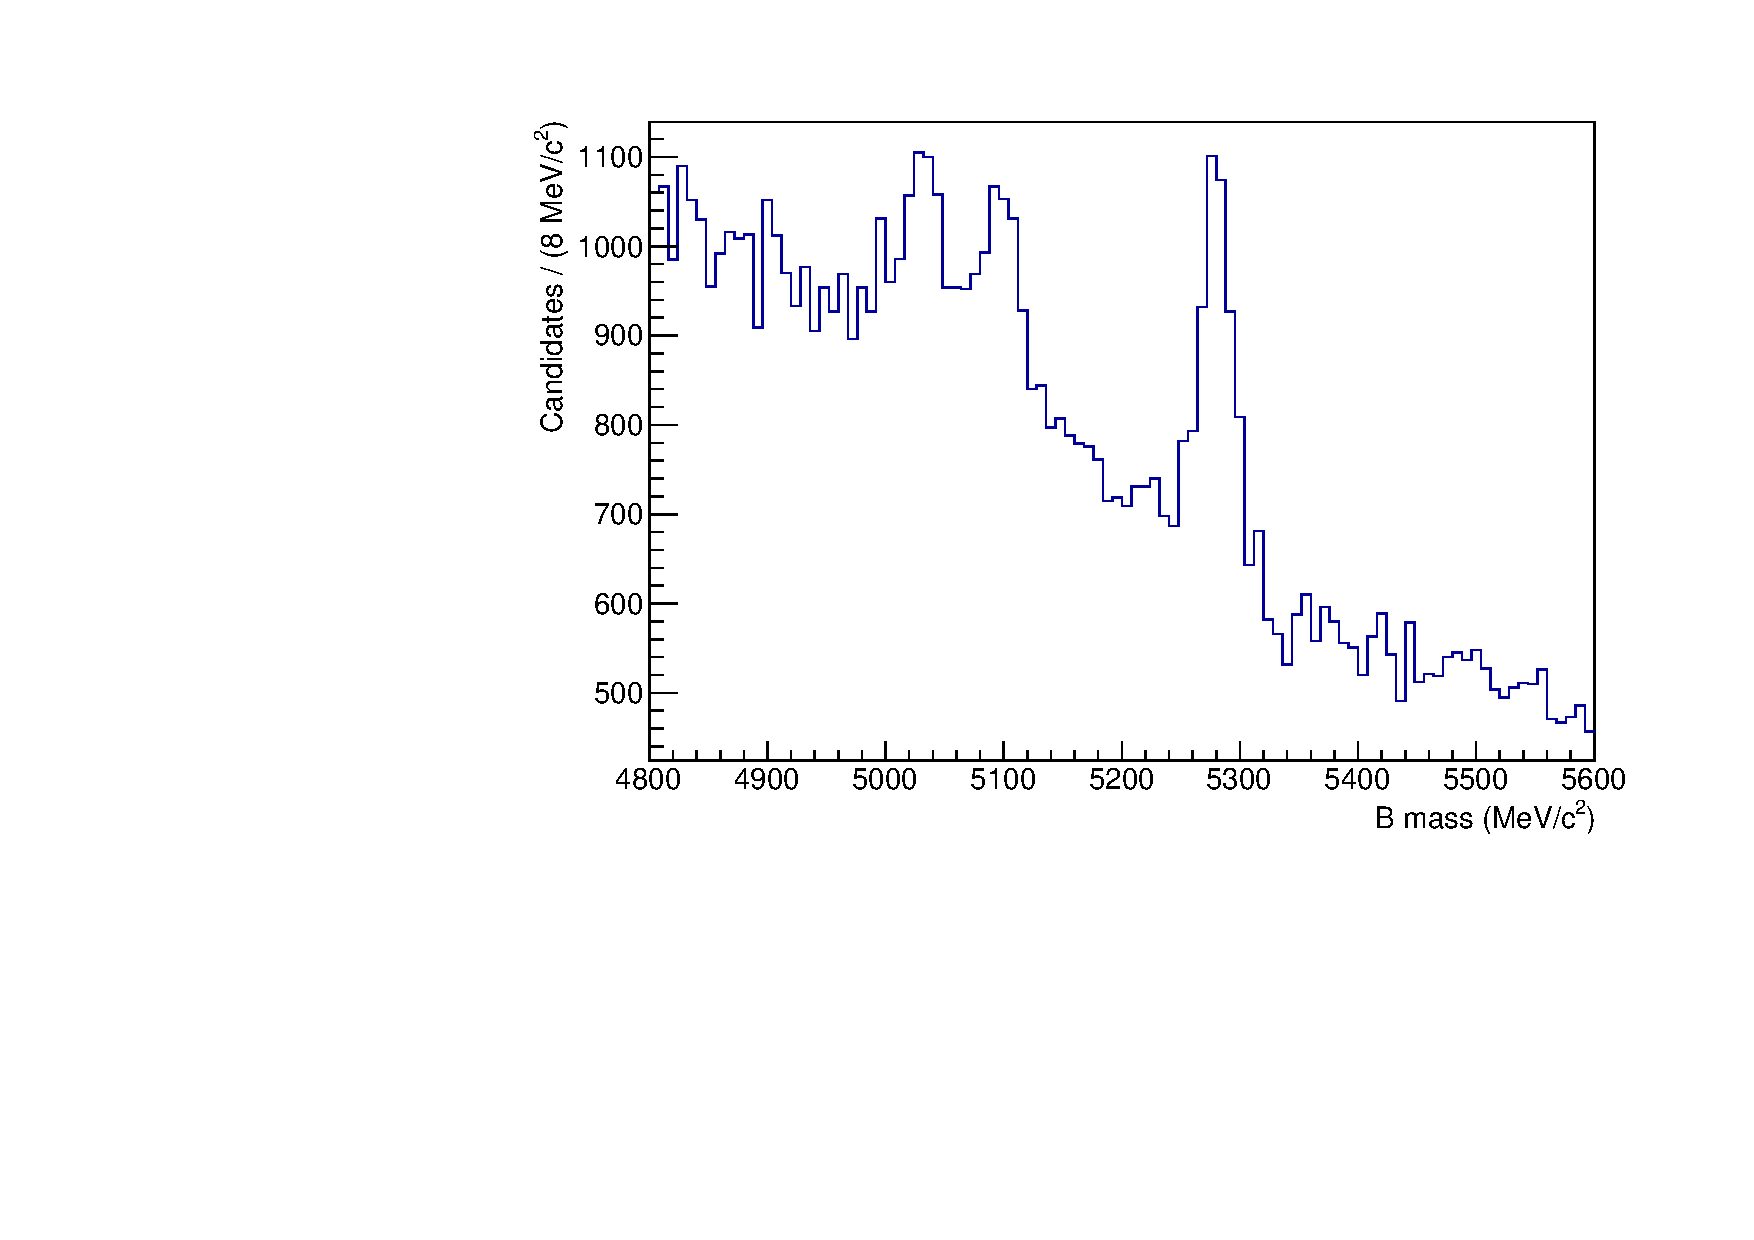
\includegraphics[width=0.6\linewidth]{figures/selection/DataDD_KPi_beforeBDT.pdf}
\caption{The refitted \Bm mass distribution for \kpi DD candidates in \runtwo after the stripping and mass requirements on intermediate states. The \Bm signal peak can be seen at the known \Bm mass (5279 \mevcc) and the peaks at lower reconstructed \Bm mass are discussed later in Secion \ref{sec:backgrounds:partreco}.}
\label{fig:BmassbeforeBDT}
\end{figure}

\subsection{Multivariate analysis with a Boosted Decision Tree}
\label{sec:selection:bdt}

Various selection requirements can be placed on variables relating to individual particles in the decay chain. As these variables tend to be correlated with each other, the separation power can be improved by using a multivariate analysis (MVA) method, which exploits these correlations between the variables. The MVA implemented in this analysis is a Boosted Decision Tree (BDT)~\cite{Breiman}. Decision trees take a given set of variables from signal and background training samples and construct an algorithm to decide whether a given event corresponds to signal or background. Firstly, the best variable and value is found to split events into two subsets in order to separate signal and background, the process is then repeated for each of the two subsets. This is continuously repeated in order to build a tree, where the nodes at the end are called leaves. If more than half of the weight of a leaf corresponds to signal, it is a signal leaf, where each event is given a value of +1, otherwise it is a background leaf, where each event is given a value of -1. Signal events on a background leaf and background events on a signal leaf are misclassified. In order to stablilise this process many trees are built to construct a weighted average over all the trees. After each tree is built, the misclassified events are reweighted (boosted) and a new tree is build with the rewighted events. The boosting makes misclassified events more likely to be correctly classified in future trees; a particular type of boosting, called gradient boost, is used in this analysis. The result of the process assigns each event a weight from -1 (most background-like) to +1 (most signal-like). 

\subsubsection{Training samples}

A Boosted Decision Tree (BDT) with the gradient boost (BDTG) method using the Toolkit for Multivariate Analysis (TMVA) framework~\cite{TMVA} is employed in order to reduce the combinatoric background level. A separate BDT is trained for LL and DD candidates, named BDTG\_LL and BDTG\_DD respectively. The BDTs are mainly based on topological variables, so are insensitive as to whether the \Dz daughters are kaons or pions. Therefore, the same BDT is used for all of the two-body \Dz decay modes, trained using \kpi decays, and another BDT is used for all of the four-body \Dz decay modes, trained using \kpipipi decays. For the two body modes, simulated 2011 and 2012 samples for the decay \kpi were used to provide a signal sample. Events in the favoured \kpi mode, from 2011 and 2012 data, in the region of \Bm mass above 5600 MeV were used as a sample of background combinatoric events. 

As there are five tracks in the final state of \kpi the reconstruction efficiency of this decay mode is very low. The number of simulated events passing the stripping and going on to be used as a signal training sample was found to be too small, which resulted in overtraining of the BDT. In order to deal with this problem, a simulated sample was produced with selection applied at the point of generation, known as generator level selection. The effect of this is that events that were not likely to pass the offline stripping selection and reconstruction are removed before the computationally intensive process of simulating the event in the \lhcb detefctor. These generator level selection requirements, detailed in Table \ref{table:generatorlevel}, result in significantly higher proportion of generated events passing the stripping, giving a larger signal sample size to be used in training.

\begin{table}
\centering
\begin{tabular}{cc}
Variable & Selection \\
\hline
Bu $p$ & 50 \gevc \\
Bu $p_T$ & 4.5 \gevc \\
Bu $\tau$ & 0.4 \ps \\
\Dz p & 20 \gevc \\
\Dz $p_T$ & 2 \gevc \\
$K_s\ p$ & 4.5 \gevc \\
$K_s\ p_T$ & 0.45 \gevc \\
Bach $p$ & 5.5 \gevc \\
Bach $p_T$ & $5.5$ \gevc \\
$K_s$ daughters $p$ & 2 \gevc \\
\Dz daughters $p$ & 1.5 \gevc \\
\end{tabular}
\caption{Selection applied at generation level before events are simulated in the \lhcb detector. Variables are required to be larger than the values given.}
\label{table:generatorlevel}
\end{table}

The generator level selection removes 89\% of events at generator level while keeping 78\% of LL candidates and 81\% of DD candidates. Not all generator level selections are looser than those applied to the data in stripping, however the loss in good signal was deemed to be acceptable to be able to increase signal yields in the simulated sample. Any signal efficiencies required in this analysis are calculated from simulated signal samples with no generator level selection applied.

For \kpipipi, simulated 2015 and 2016 samples were produced for training a BDT designed for four-body modes. A large \runtwo simulated sample was generated in order avoid overtraining of the 4 body BDT. This allows training of the BDT without having to apply selections to the sample at the generator level. A signal sample of simulated 2015 and 2016 events for the decay \kpipipi was used. Events in the favoured \kpipipi mode, from 2015 and 2016 data, in the region of \Bm mass above 5600 MeV were used as a sample of background combinatoric events. All samples used in training the BDTs are split into a training and testing sample before being used as an input to the multivariate algorithm.

\subsubsection{Setup and implementation of the multivariate algoritm}

Initial selection requirements are applied to both the signal and background training samples to remove candidates that would not pass the final selection. This allows a more accurate discrimination between signal and background in data. The selection criteria on the training samples are:

\begin{itemize}
\item The \chisq of the decay chain refit per degree of freedom, $\chisq_\text{refit}$, with {\tt D0const}, {\tt KS0const} and {\tt PVconst} constraints, must lie between 0 and 100
\item The \chisqip of the \Bm candidate, with respect to the \Bm vertex, must lie between 0 and 100
\item The reconstructed \Kstarm mass must lie within 500\mev of the known \Kstarm mass
\item The reconstructed \KS mass must lie with 15\mev of the known \KS mass for LL candidates and 20\mev for DD candidates
\end{itemize}

Various input variables are used to exploit the topology of the decay; of particular importance are the \chisq per degree of freedom of the decay chain refit, with {\tt D0const}, {\tt KS0const} and {\tt PVconst} constraints, $\chisq_\text{refit}$, and the $p_T$ asymmetry between the \Bm candidate and other tracks from the same PV, defined as
\begin{equation}
A_{p_T} = \frac{p_T^B - p_T^{\text{cone}}}{p_T^B + p_T^{\text{cone}}}
\label{ptasy}
\end{equation}
where $p_T^B$ is the $p_T$ of the reconstructed \Bm signal candidate and $p_T^{\text{cone}}$ is the sum of the $p_T$ of all other tracks in a cone of radius 1.50 surrounding the \Bm candidate. This is a quantitative measure of the isolation of the \Bm candidate. Some of the variables are transformed using a logarithm function to increase their separation power. Other input variables used include the logarithm of the \chisqip for the \Bm, bachelor, \Dz and all the \Dz decay products, the logarithm of the \chisqip for the \KS and both its decay products (for LL only) and the $p_T$ of the \KS candidate (for DD candidates only). The variables used in the BDT are slightly different for LL and DD candidates, as the separation power of the \KS variables significantly differs between LL and DD candidates. 

Tables \ref{BDTinputvariables2body} and \ref{BDTinputvariables4body} show the list of input variables, in the two and four-body BDTs respectively, ranked by separation power. The distributions of the two-body BDT input variables in the training signal and background samples are shown in Figures \ref{BDTinputdist2bodyLL} and \ref{BDTinputdist2bodyDD}. The equivalent distributions of the input variables for the four-body BDT are similar.

\begin{table}
\centering
\begin{tabular}{lll}
Rank & Variable in BDT\_LL & Variable in BDT\_DD \\
\hline
1 & log($\chisq_\text{refit}$) & log($\chisq_\text{refit}$) \\
2 & log(\KS \chisqip) & log(\D daughter kaon \chisqip) \\
3 & log(max \KS daughter \chisqip) & log(Bachelor \chisqip) \\
4 & \B ptasy 1.50 & \B ptasy 1.50 \\
5 & log(\D daug kaon \chisqip) & log(\D daughter pion \chisqip) \\
6 & log(Bachelor \chisqip) & log(\D \chisqip) \\
7 & log(\D \chisqip) & log(\B \chisqip) \\
8 & log(min \KS daughter \chisqip) & \KS $p_T$ \\
9 & log(\D daug pion \chisqip) & - \\
10 & log(\B \chisqip) & - \\
\end{tabular}
\caption{Ranking for variables for BDTG\_LL and BDTG\_DD for the two-body BDTs.}
\label{BDTinputvariables2body}
\end{table}

\begin{table}
\centering
\begin{tabular}{lll}
Rank & Variable in BDT\_LL & Variable in BDT\_DD \\
\hline
1 & log($\chisq_\text{refit}$) & log($\chisq_\text{refit}$) \\
2 & log(\KS \chisqip) & $A_{\pt}$ \\
3 & $A_{\pt}$ & log(\B \chisqip) \\
4 & log(\B \chisqip) & log(Bachelor \chisqip) \\
5 & log(\D \chisqip) & \KS $p_T$ \\
6 & log(\D daughter kaon \chisqip) & log(\D \chisqip) \\
7 & log(Bachelor \chisqip) & log(max \D daughter \chisqip) \\
8 & log(min \D daughter \chisqip) & log(\D daughter ss \chisqip) \\
9 & log(max \KS daughter \chisqip) & log(\D daughter kaon \chisqip) \\
10 & log(\D daughter ss \chisqip) & log(min \D daughter \chisqip) \\
11 & log(min \KS daughter \chisqip) & - \\
12 & log(max \D daughter \chisqip) & - \\
\end{tabular}
\caption{Ranking for variables for BDTG\_LL and BDTG\_DD for the four-body BDTs. The particle name "D daughter ss'' refers to the pion from the \D which has the same sign of the kaon.}
\label{BDTinputvariables4body}
\end{table}

\begin{figure}
\centering
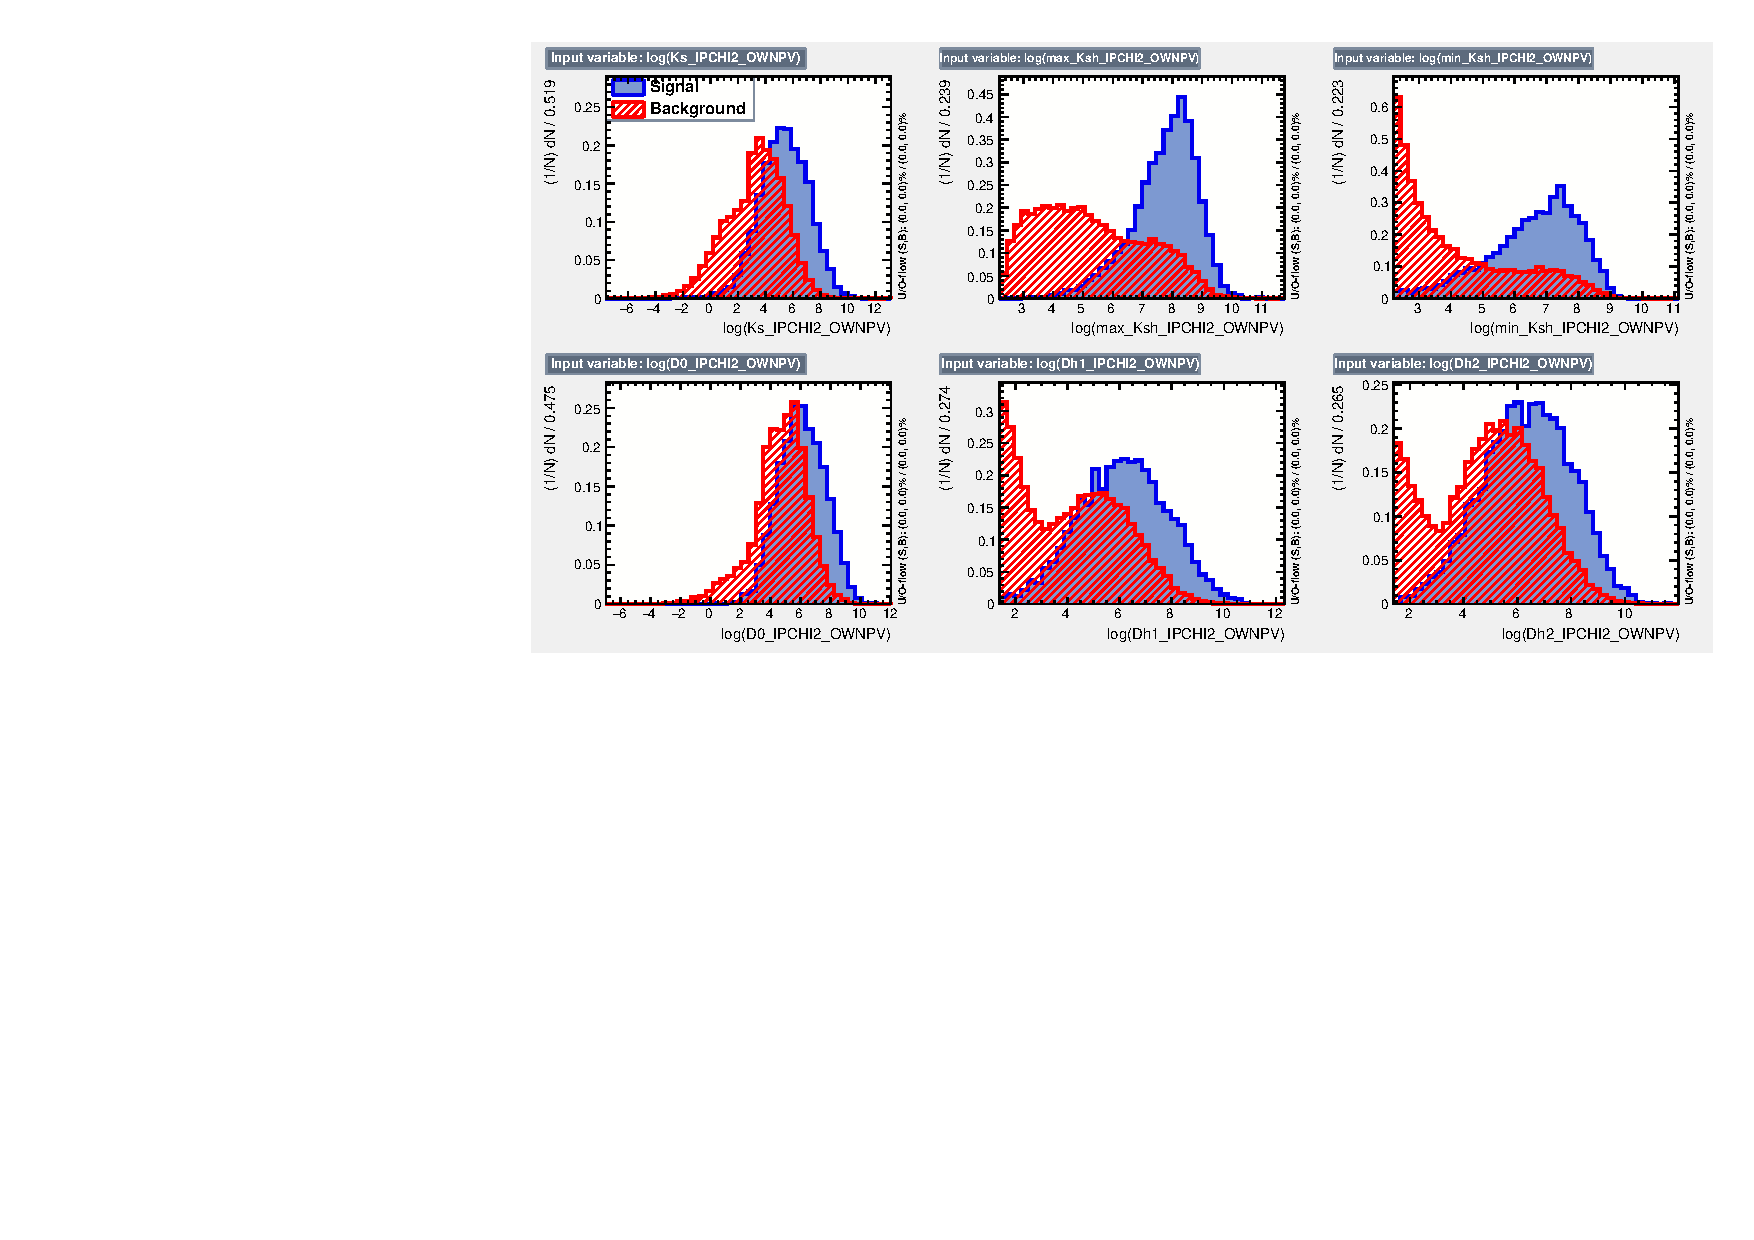
\includegraphics[width=\linewidth]{figures/selection/inputvariables_KPi_LL_run1_1.pdf}
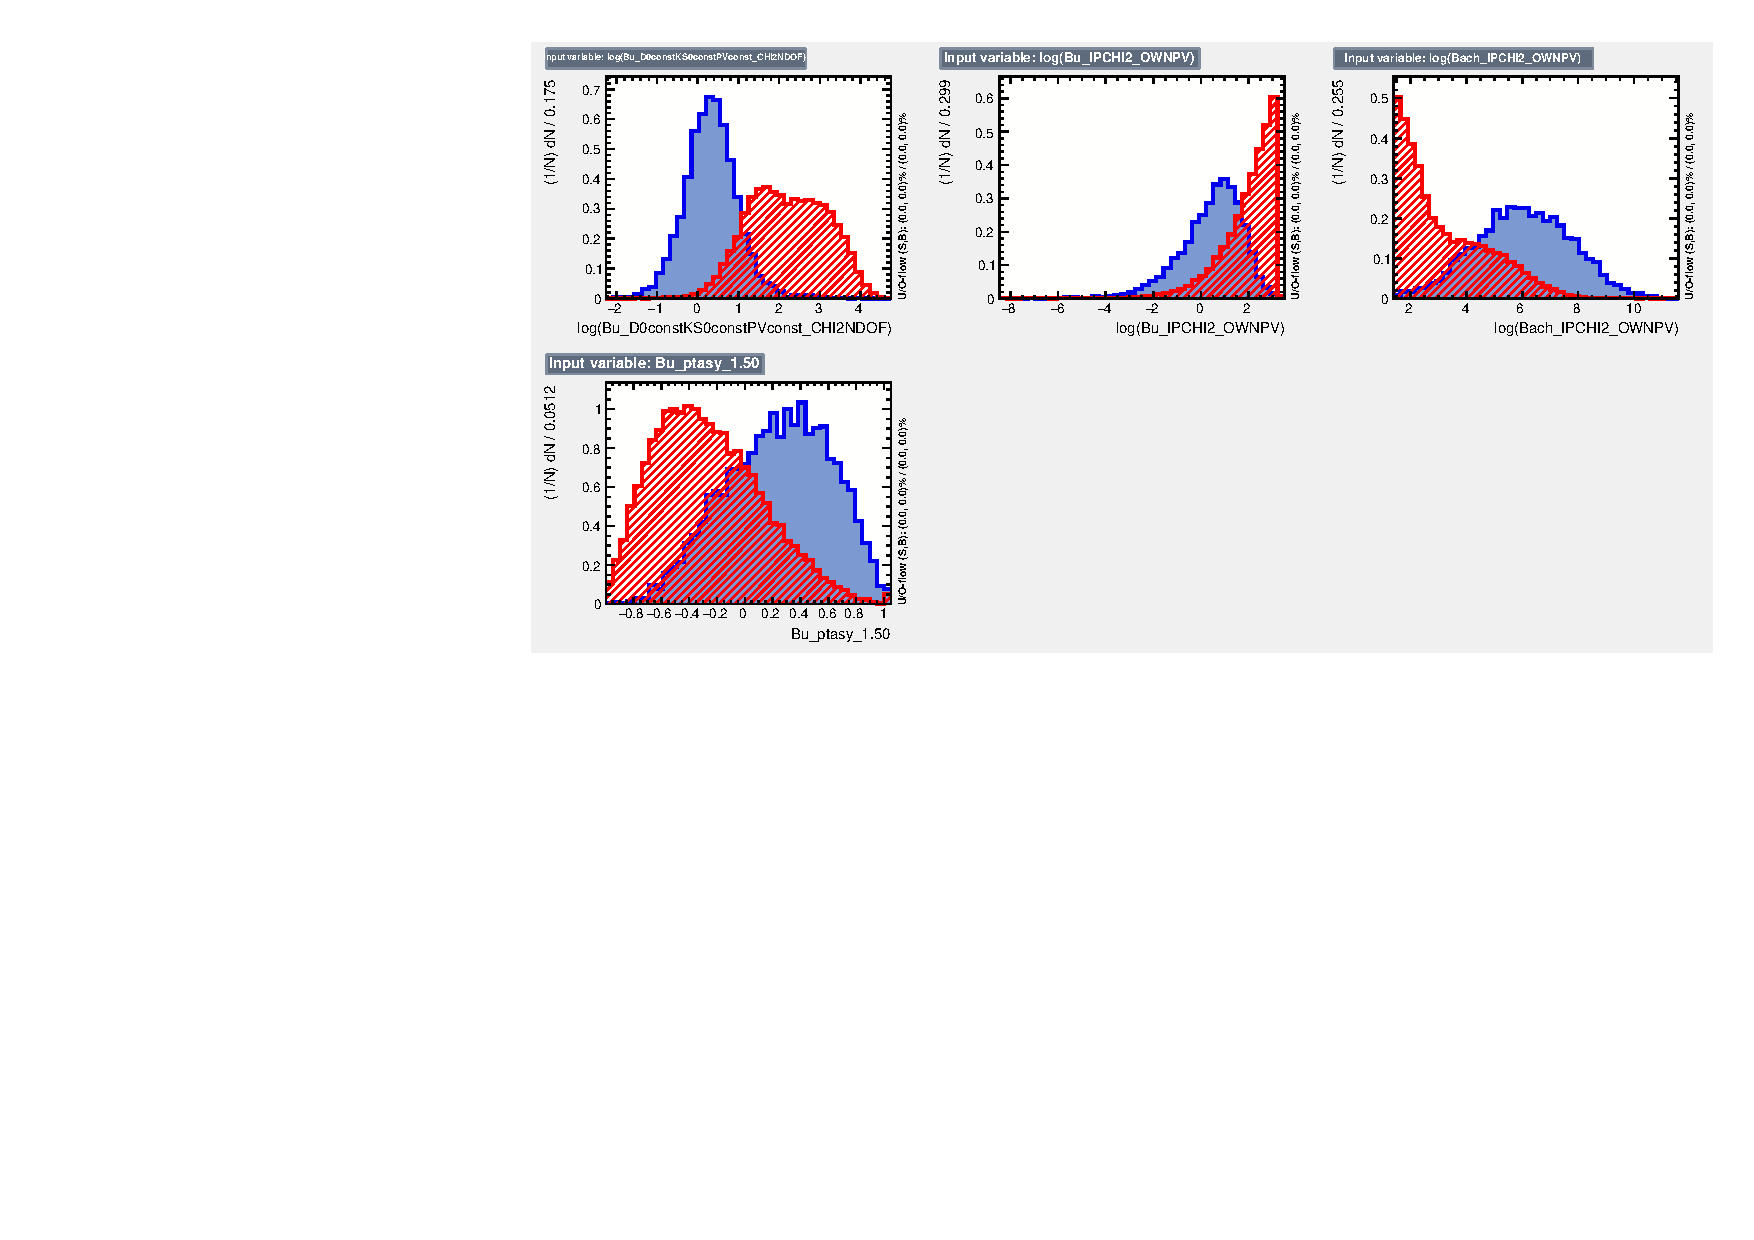
\includegraphics[width=\linewidth]{figures/selection/inputvariables_KPi_LL_run1_2.pdf}
\caption{Distributions of the input variables using the training signal and background samples for two-body LL BDT.}
\label{BDTinputdist2bodyLL}
\end{figure}

\begin{figure}
\centering
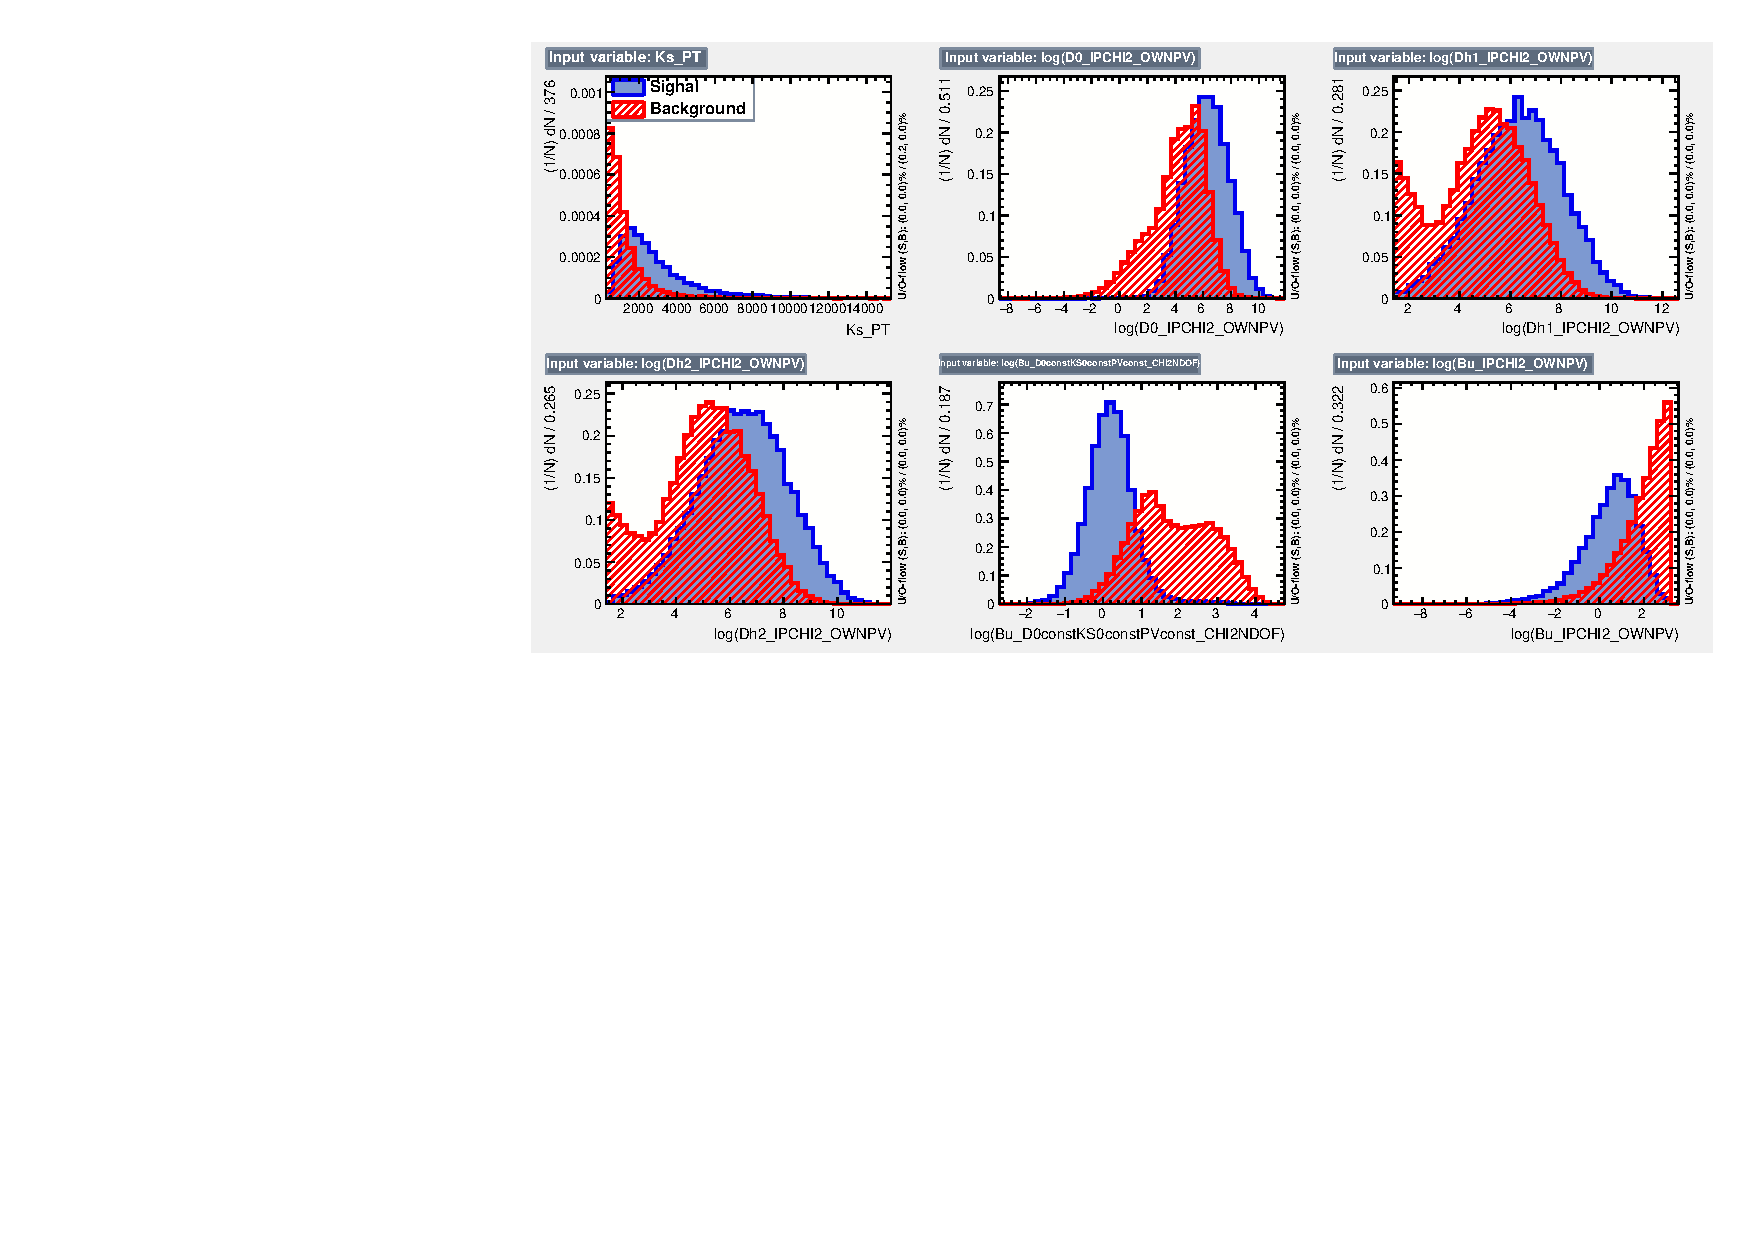
\includegraphics[width=\linewidth]{figures/selection/inputvariables_KPi_DD_run1_1.pdf}
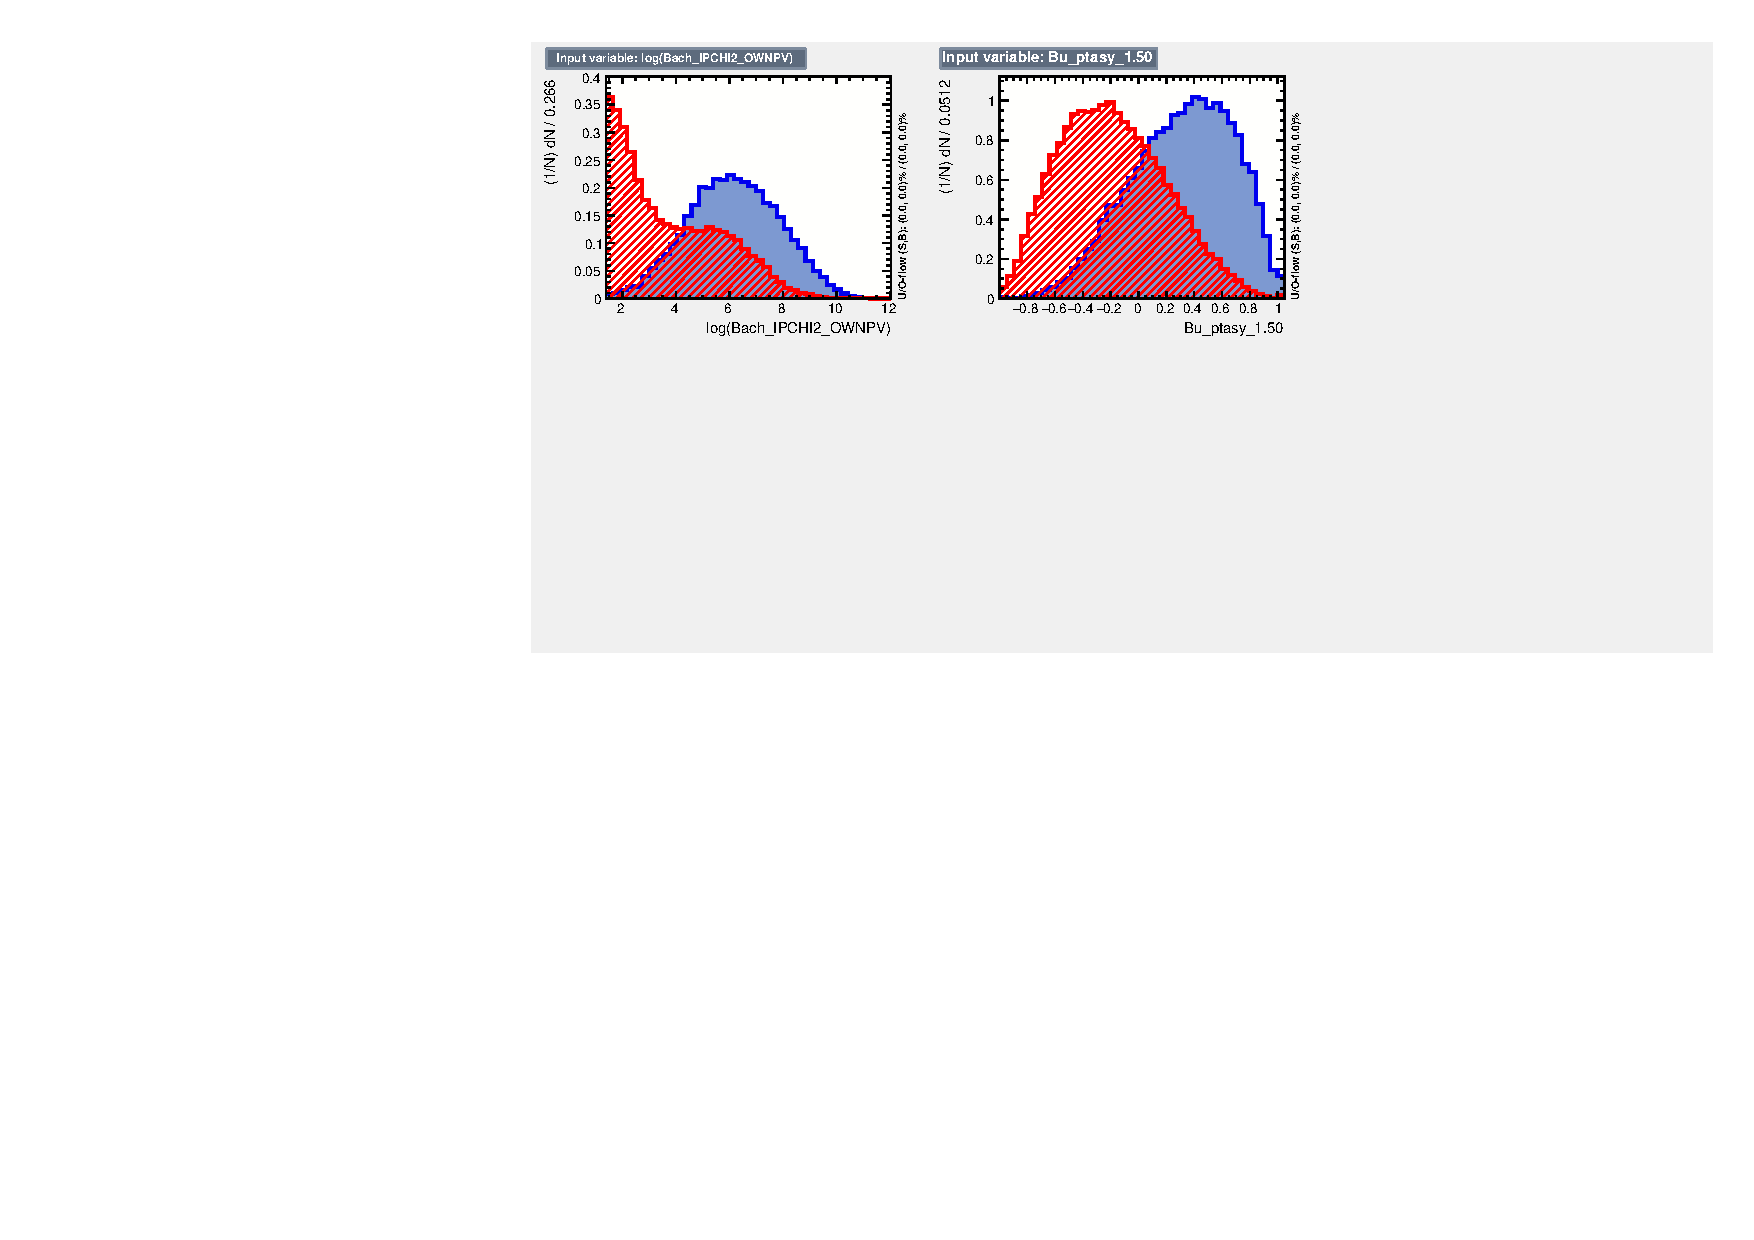
\includegraphics[trim = 0mm 50mm 0mm 0mm, clip,width=\linewidth]{figures/selection/inputvariables_KPi_DD_run1_2.pdf}
\caption{Distributions of the input variables using the training signal and background samples for two-body DD BDT.}
\label{BDTinputdist2bodyDD}
\end{figure}

%\begin{figure}
%\centering
%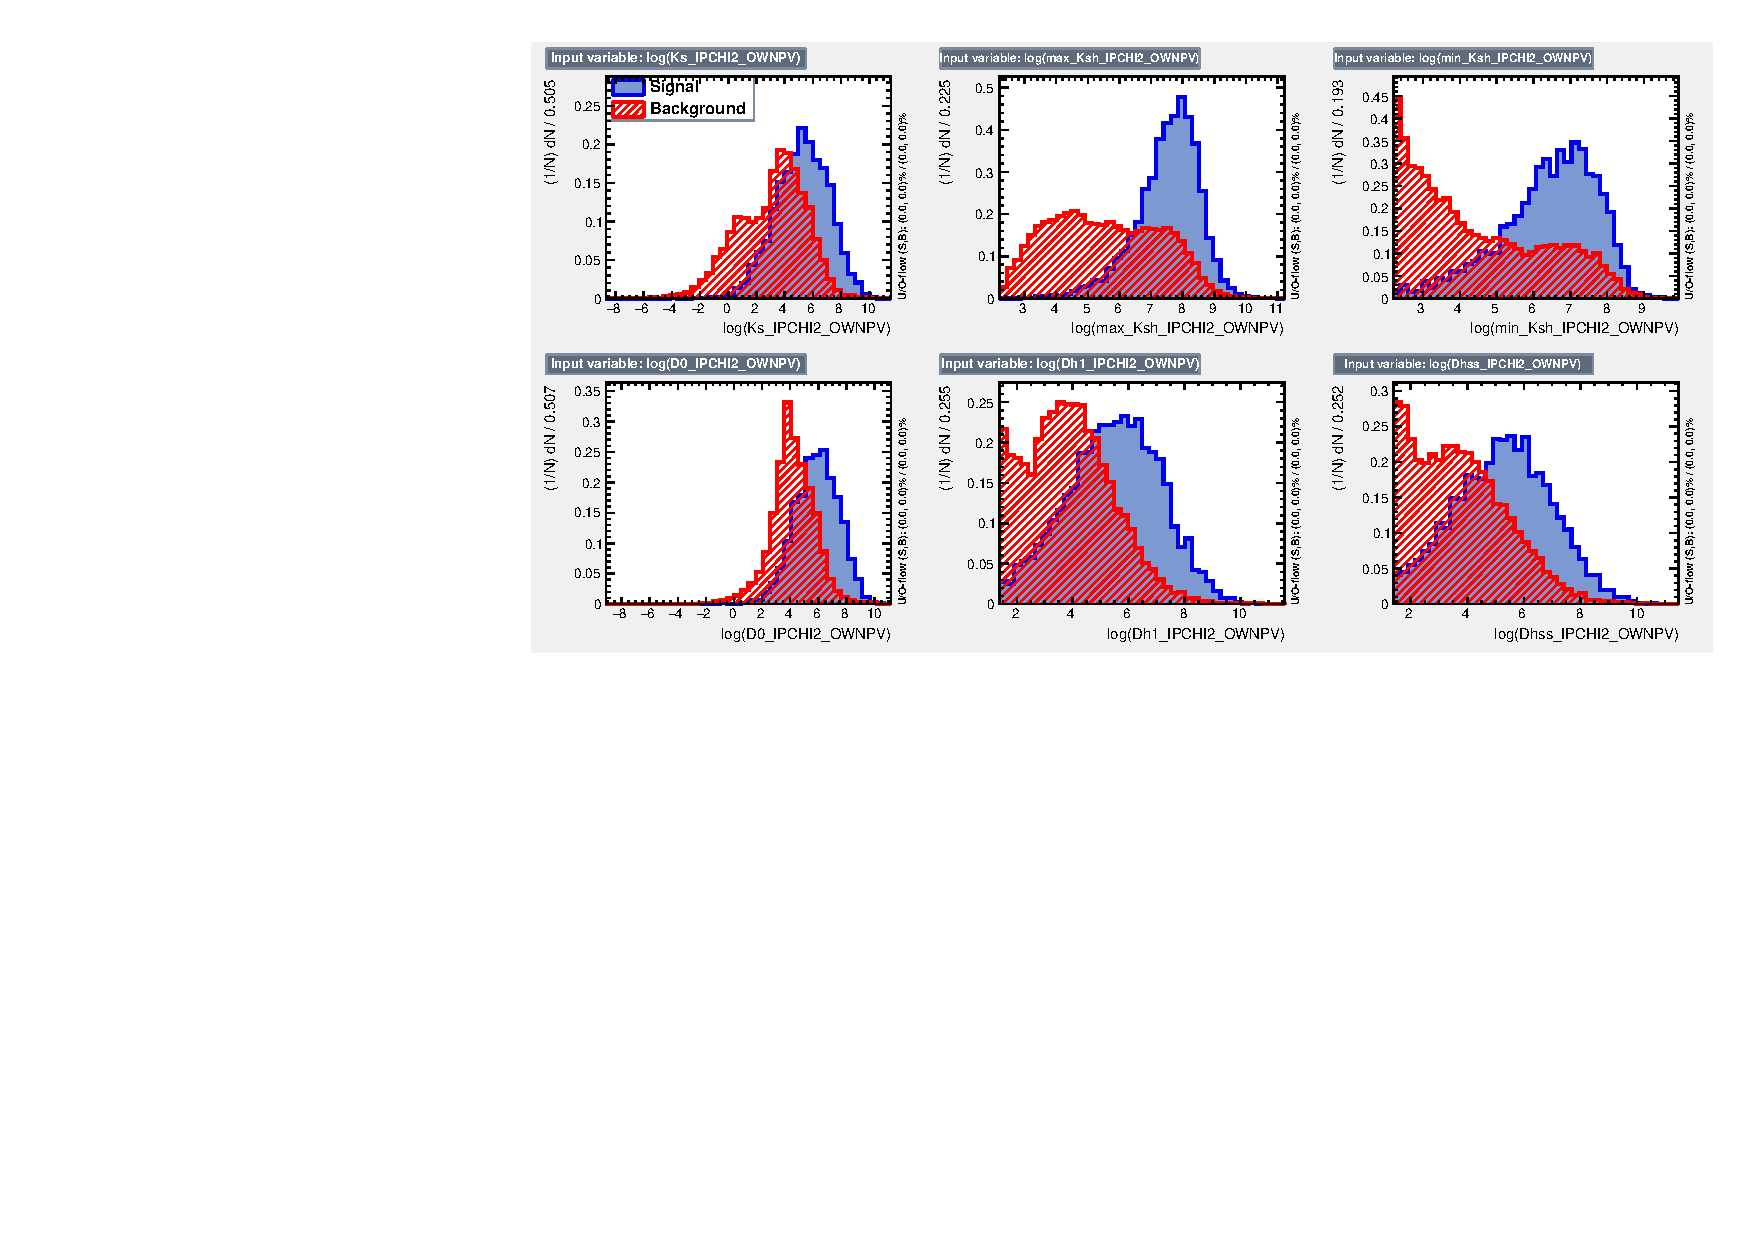
\includegraphics[width=0.8\linewidth]{figures/selection/inputvariables_KPiPiPi_LL_run2_1.pdf}
%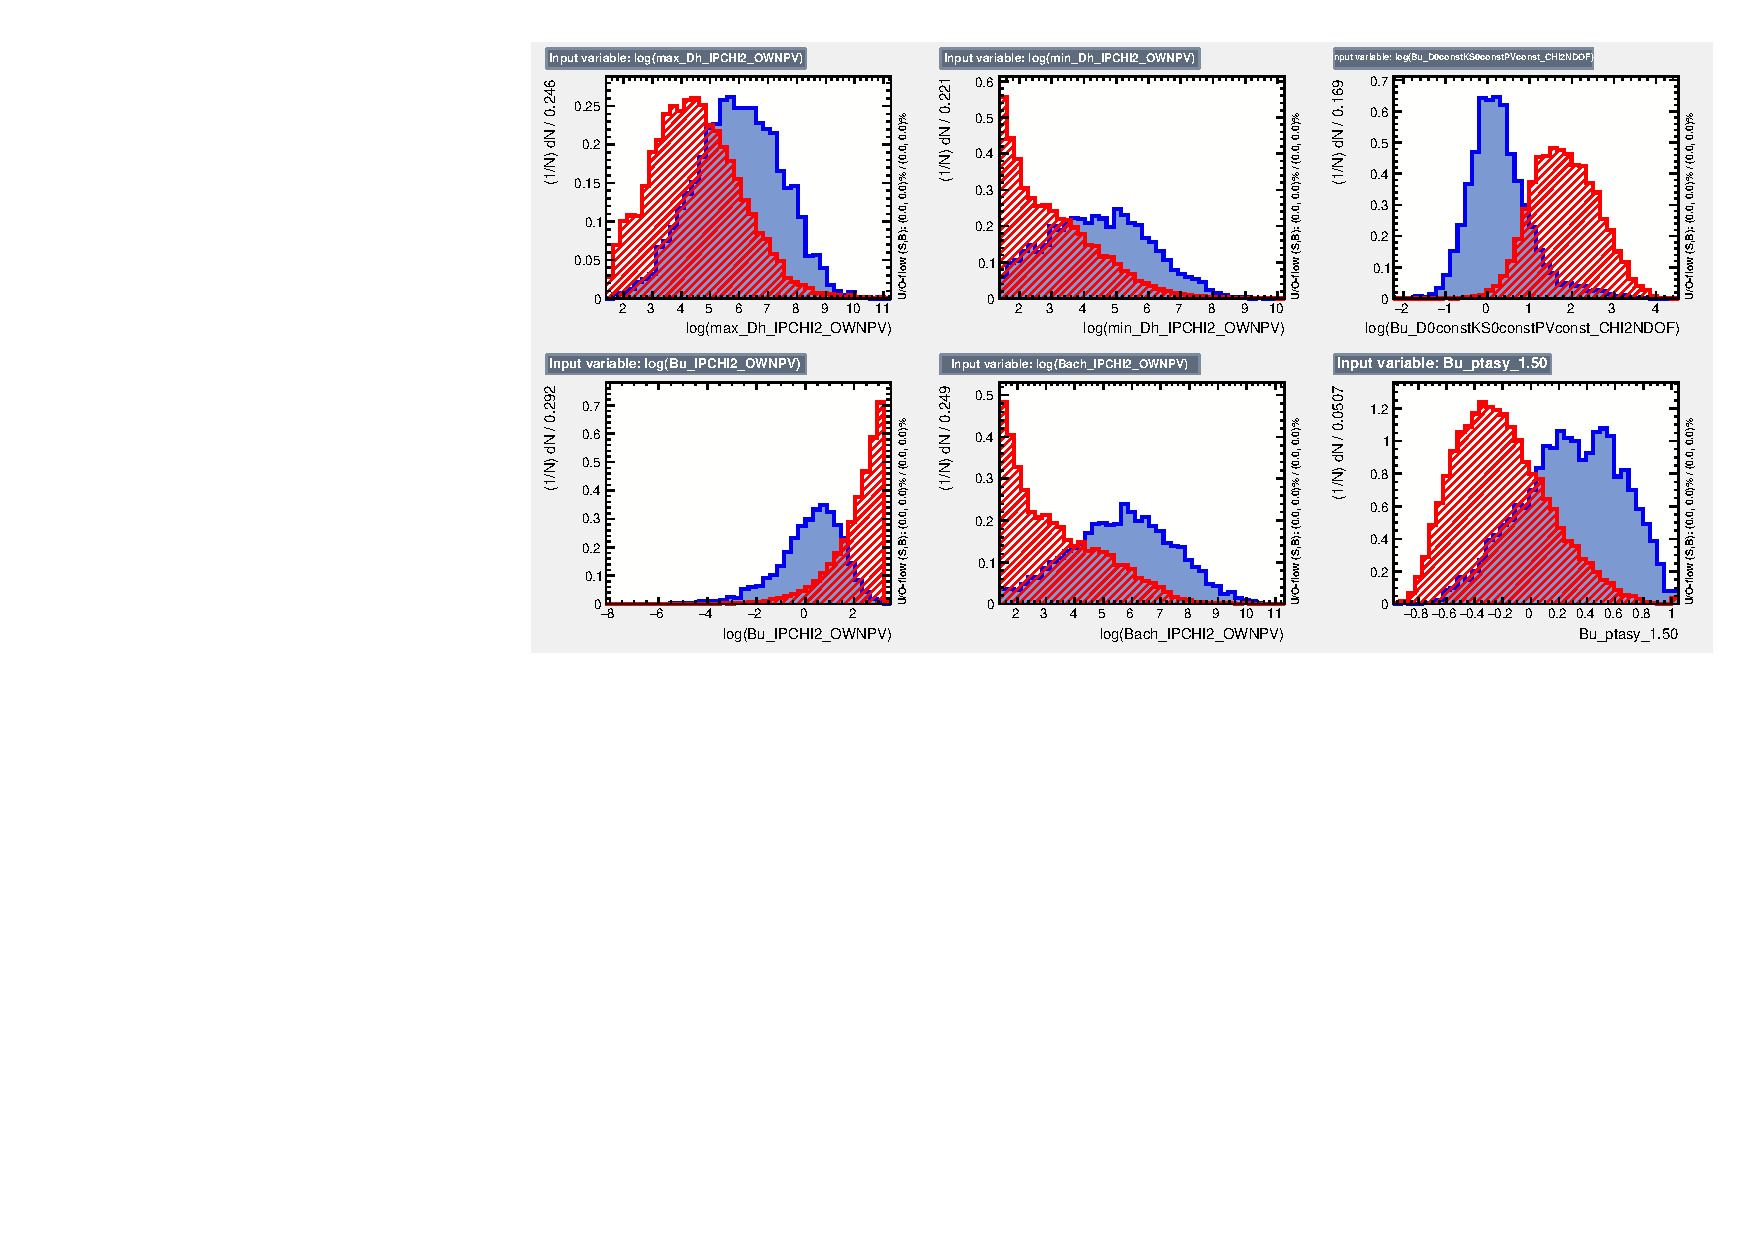
\includegraphics[width=0.8\linewidth]{figures/selection/inputvariables_KPiPiPi_LL_run2_2.pdf}
%\caption{BDT input variable distributions for signal and background for 4-body LL}
%\label{BDTinputdist4bodyLL}
%\end{figure}
%
%\begin{figure}
%\centering
%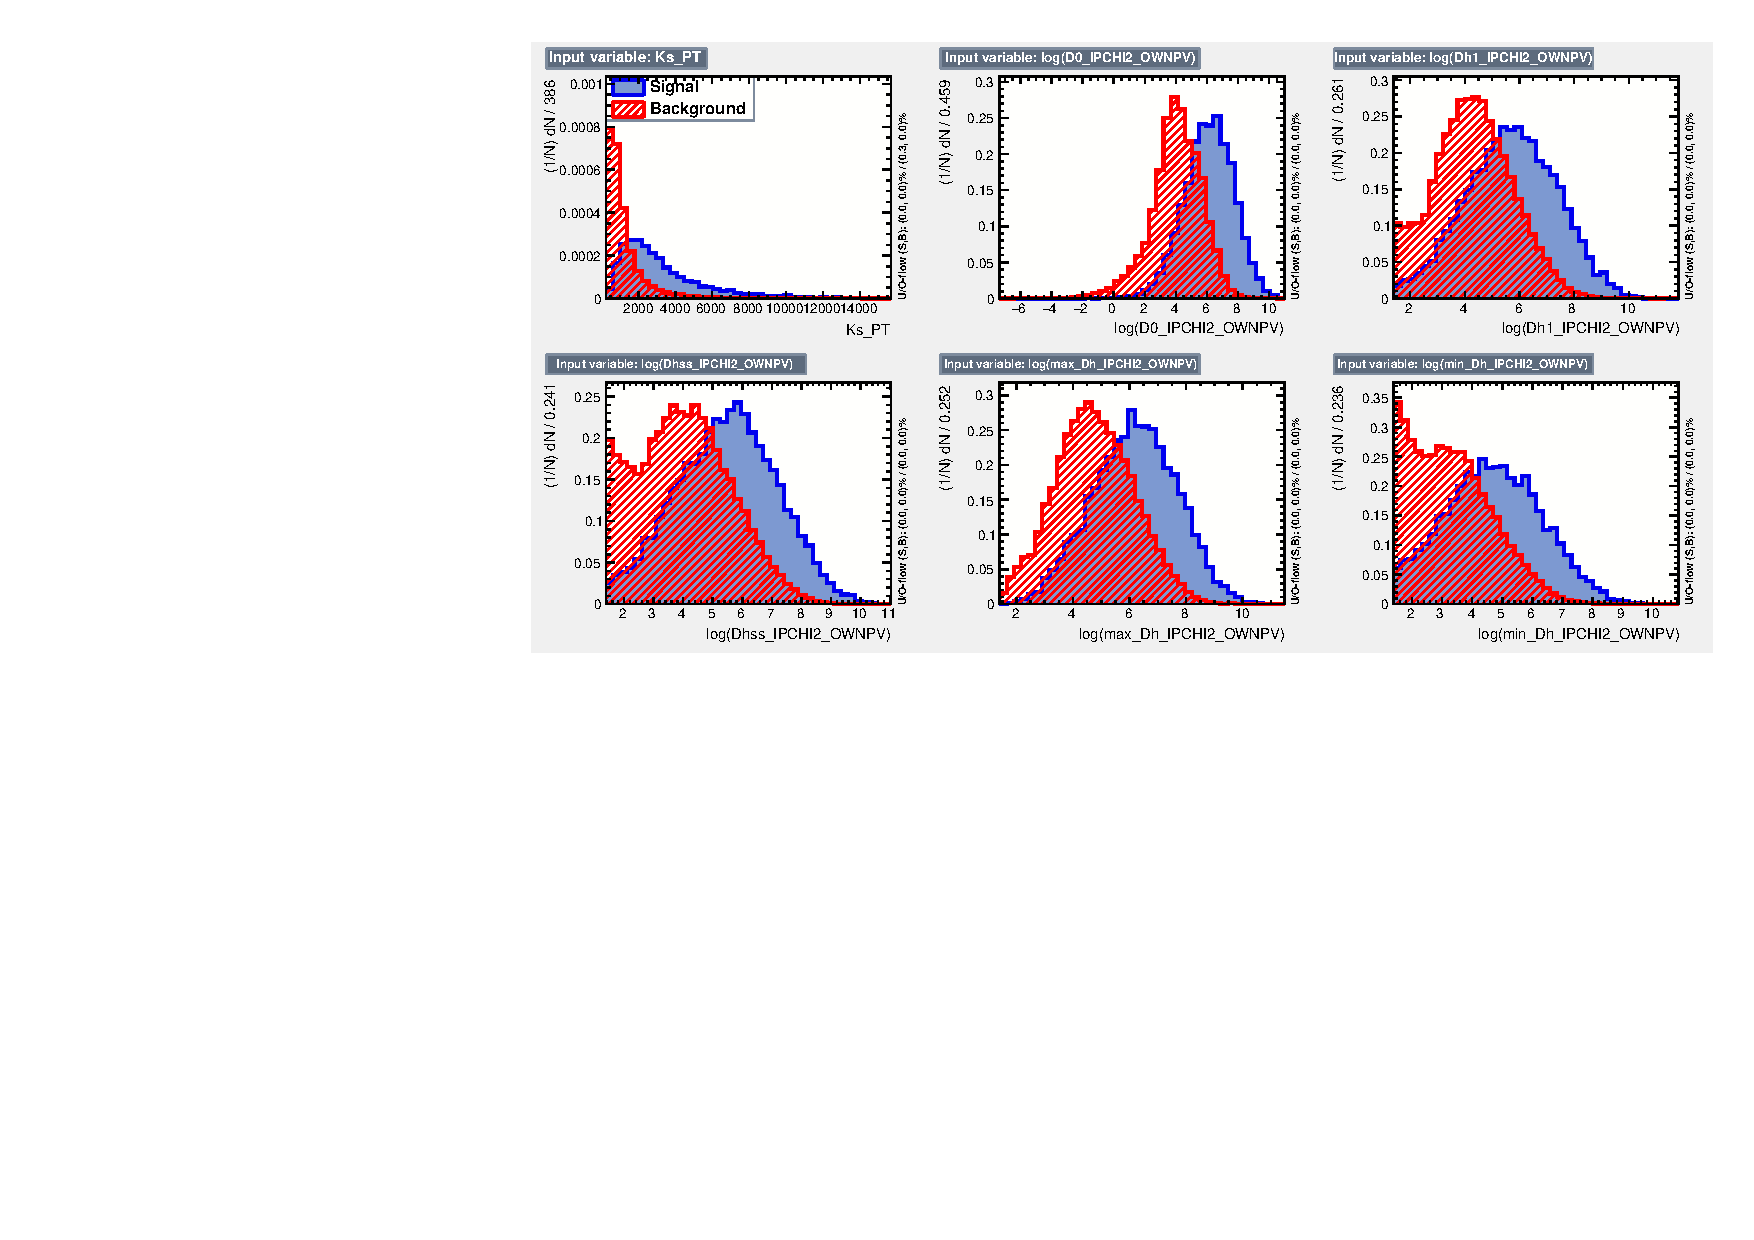
\includegraphics[width=0.8\linewidth]{figures/selection/inputvariables_KPiPiPi_DD_run2_1.pdf}
%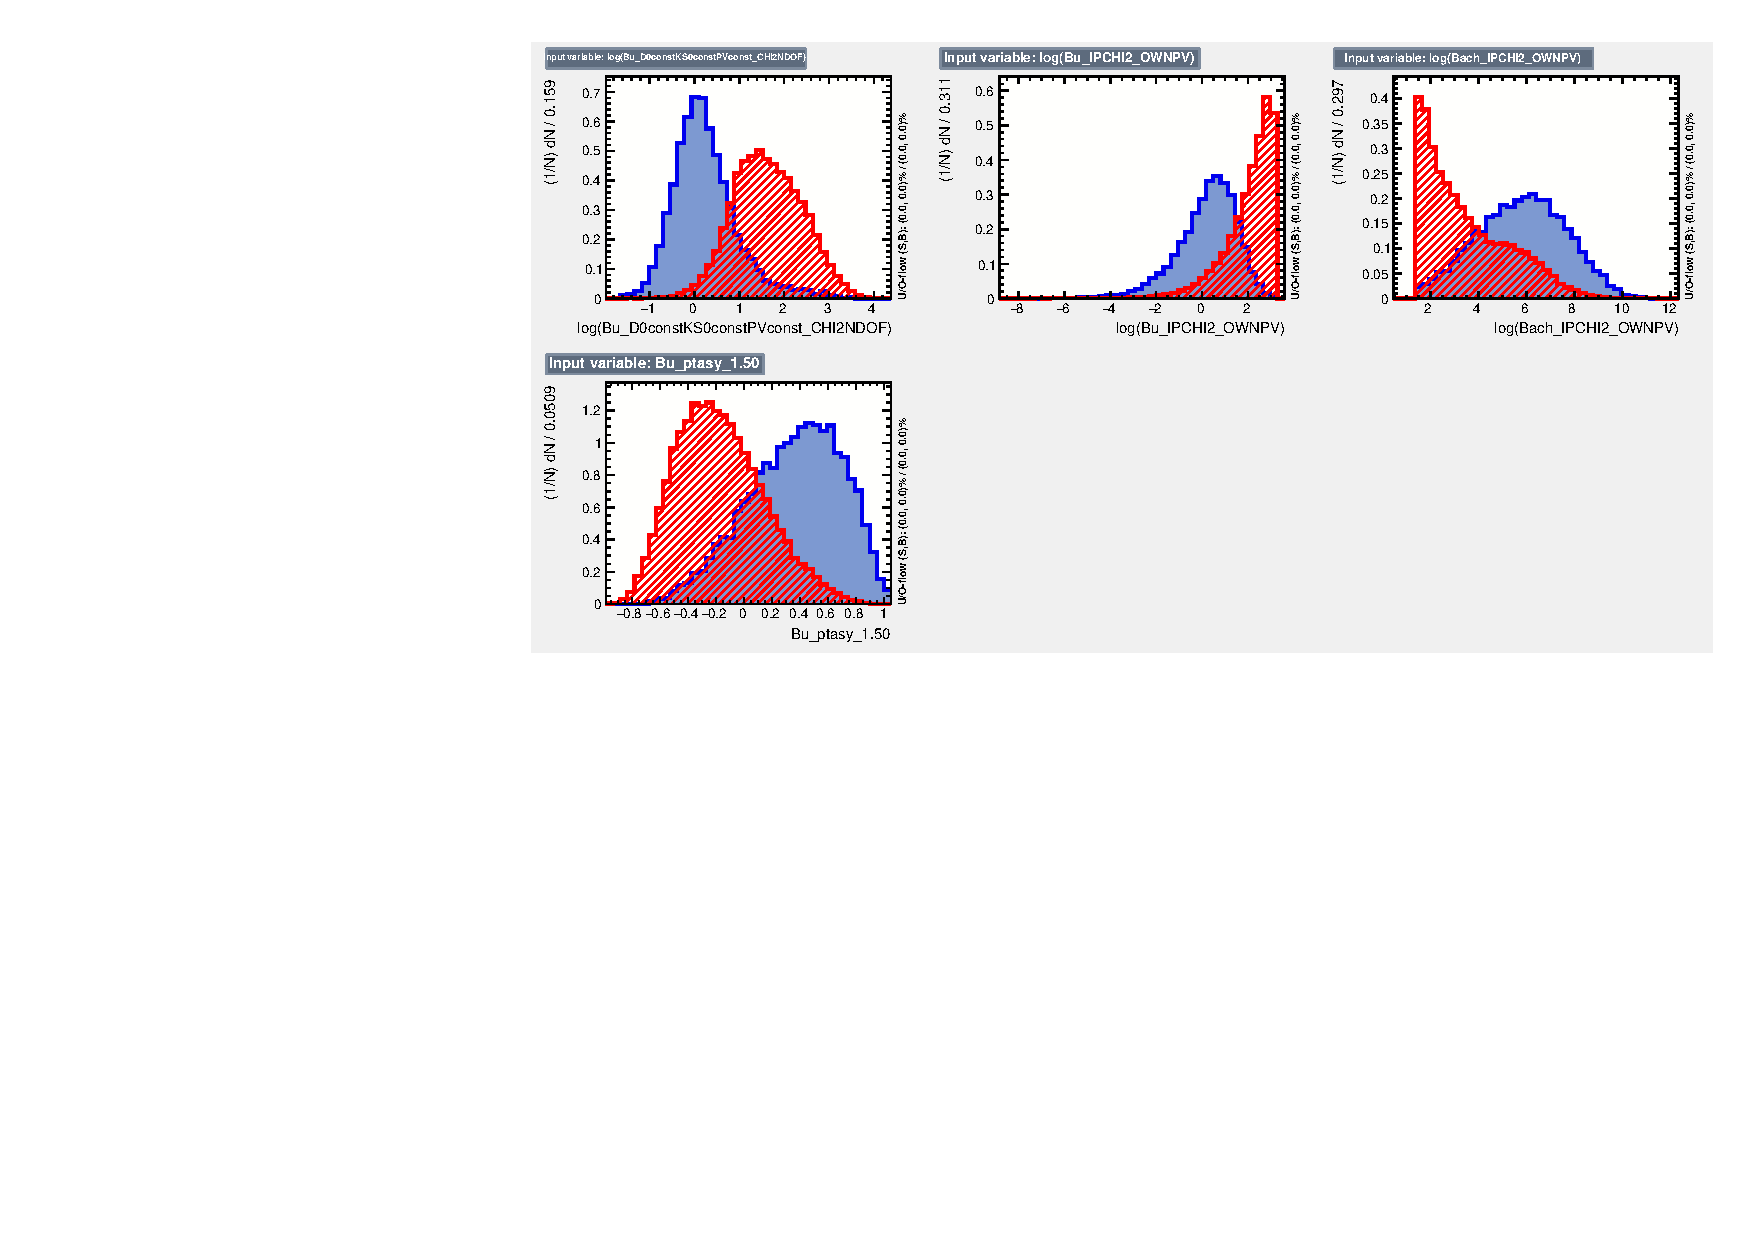
\includegraphics[width=0.8\linewidth]{figures/selection/inputvariables_KPiPiPi_DD_run2_2.pdf}
%\caption{BDT input variable distributions for signal and background for 4-body DD}
%\label{BDTinputdist4bodyDD}
%\end{figure}

%\begin{figure}[tb]
%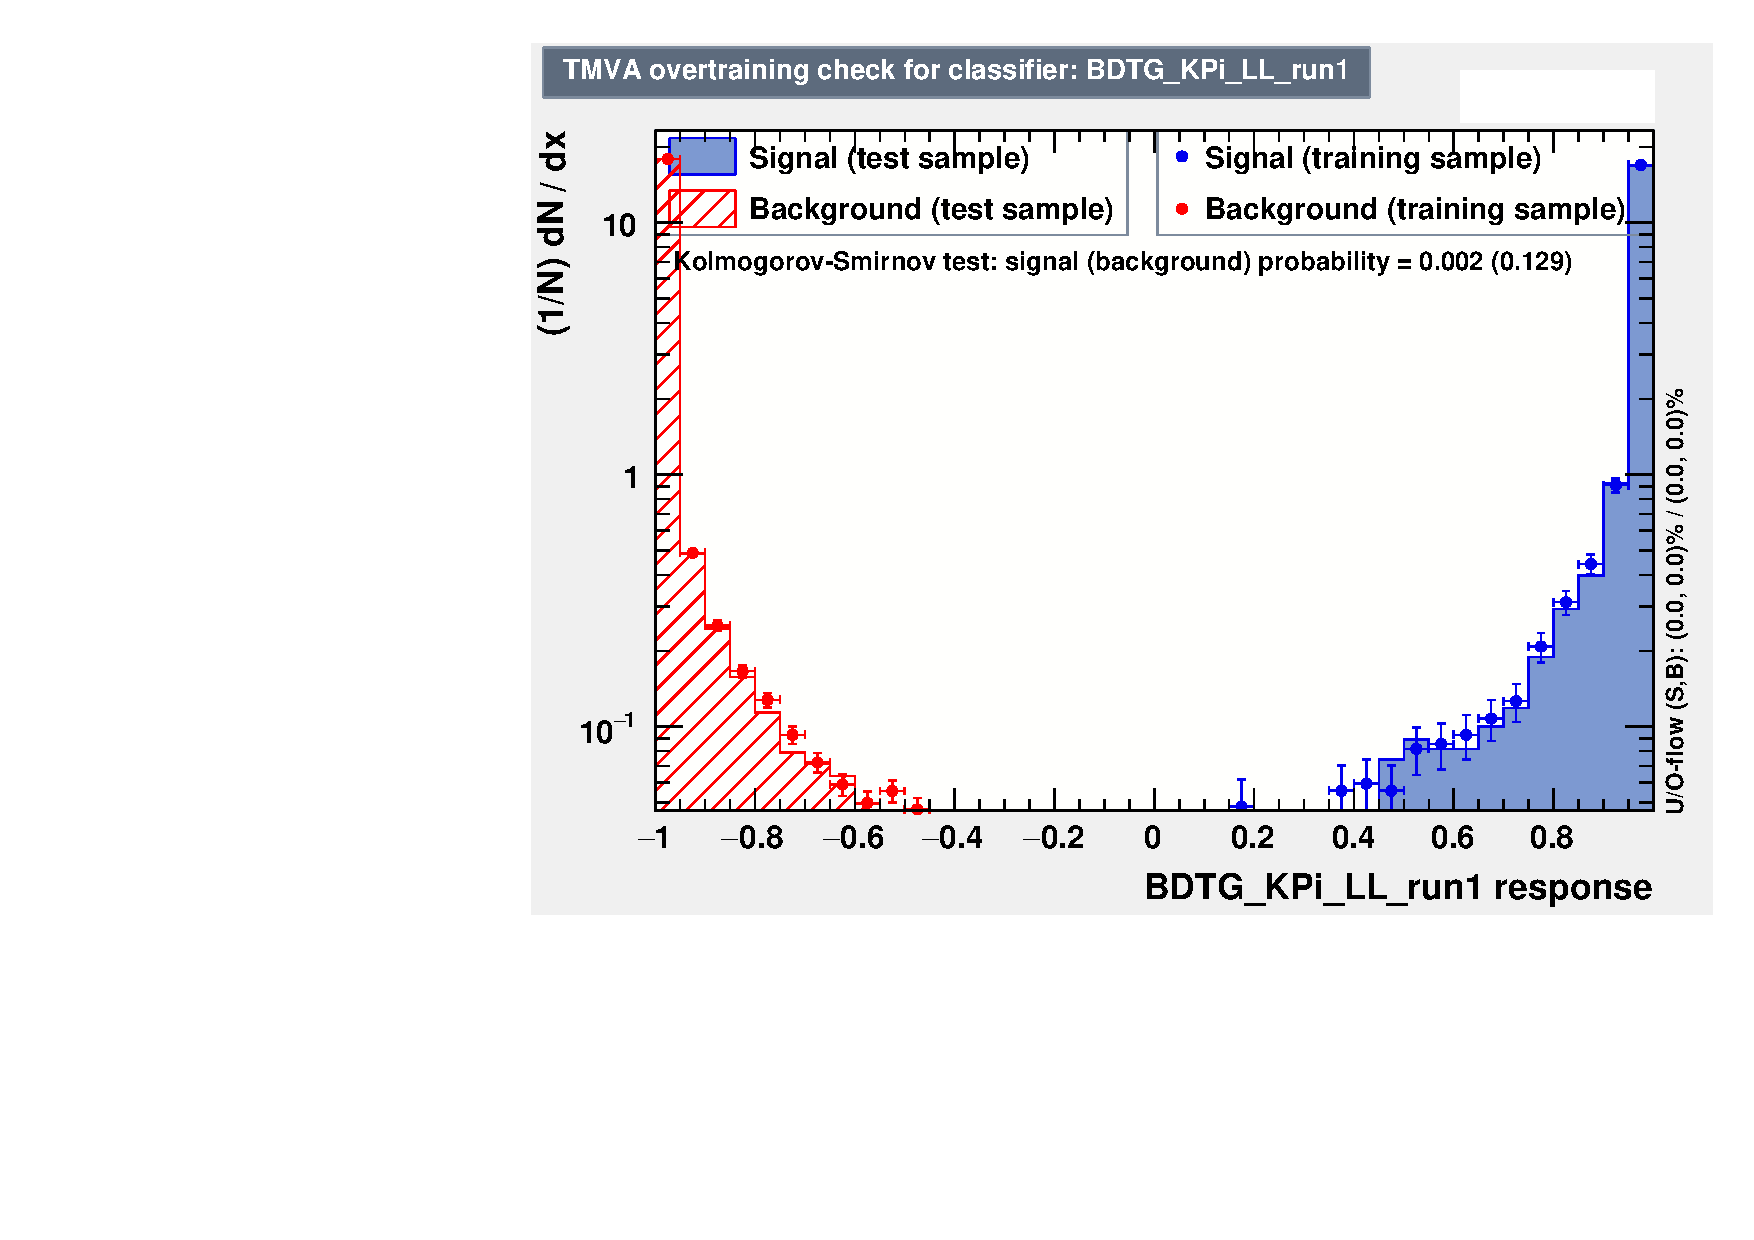
\includegraphics[width=0.5\linewidth]{figures/selection/overtraining_KPi_LL_run1.pdf}
%\put(-150,100) {(a)}
%\hfill
%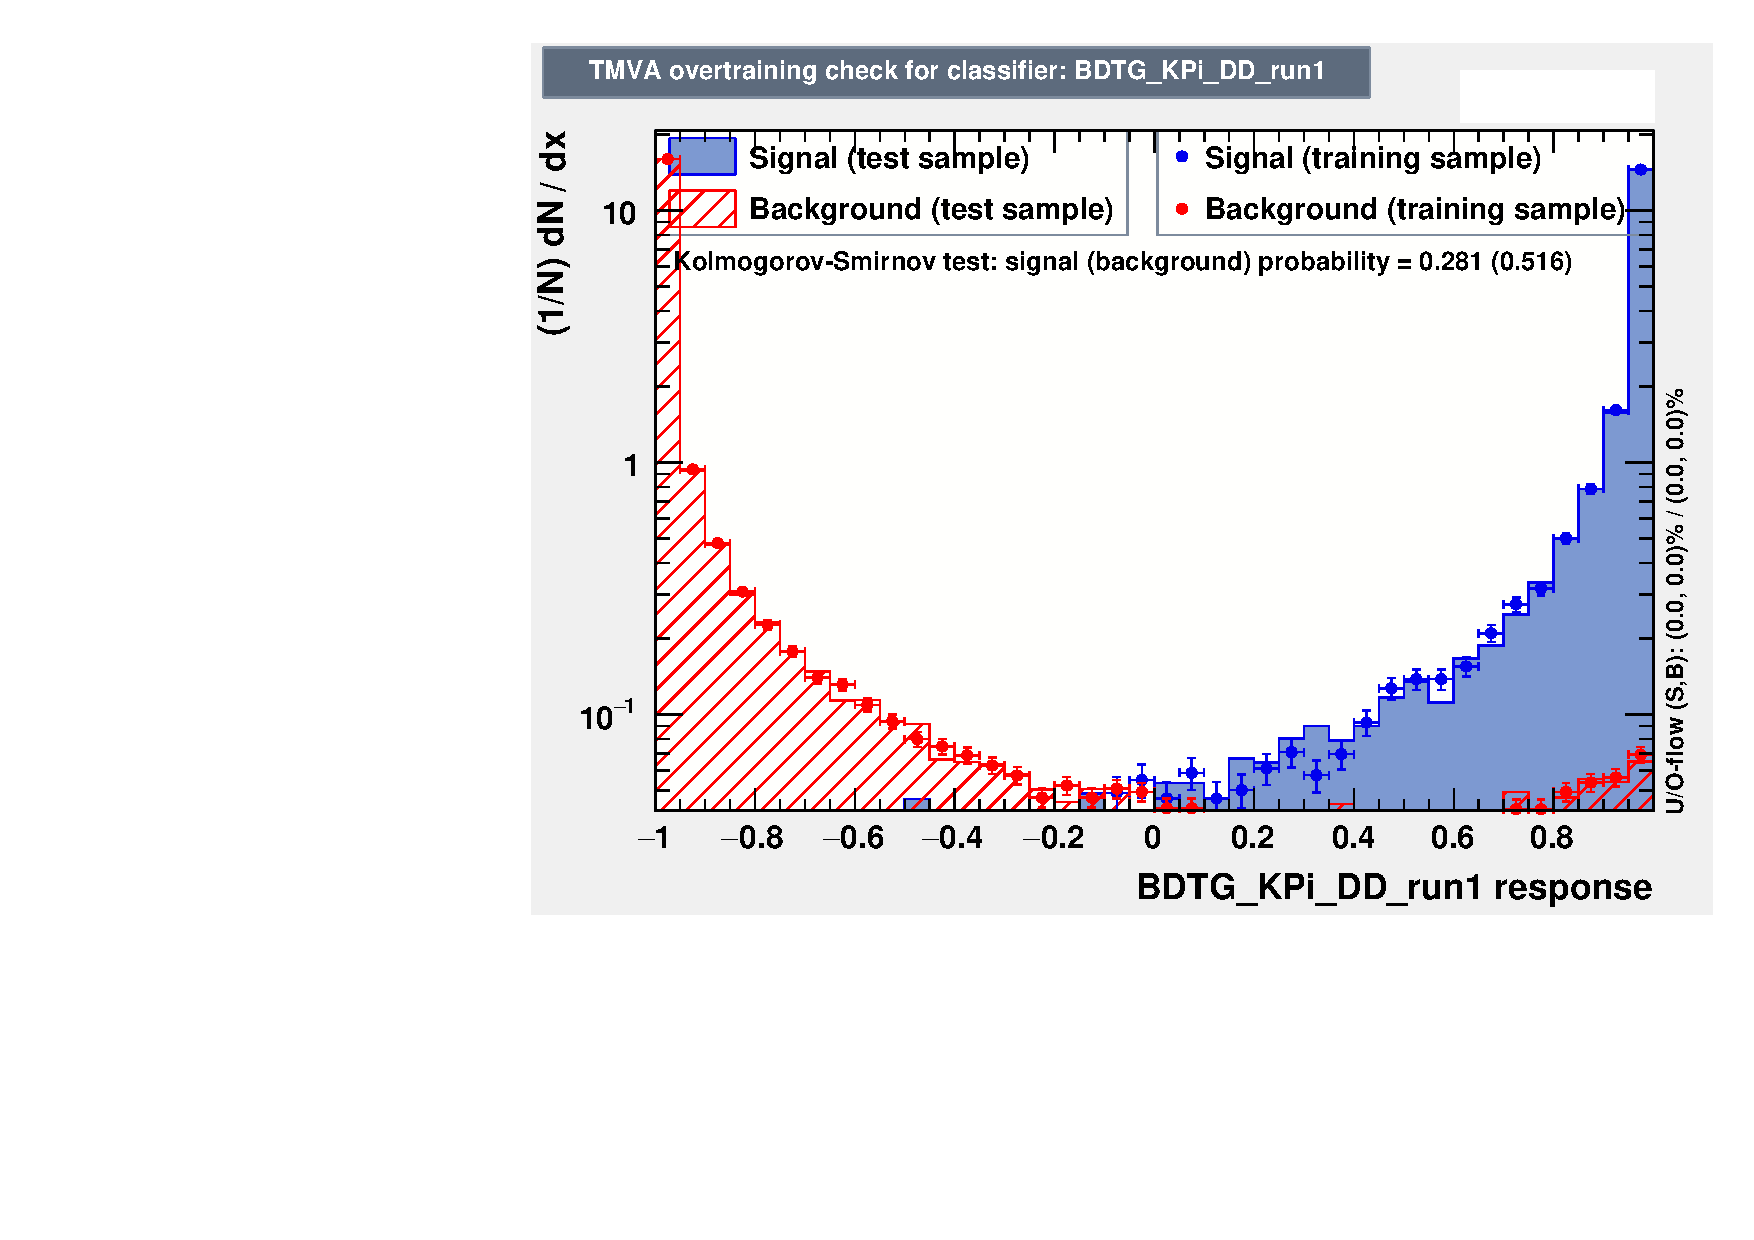
\includegraphics[width=0.5\linewidth]{figures/selection/overtraining_KPi_DD_run1.pdf}
%\put(-140,100) {(b)}
%\hfill
%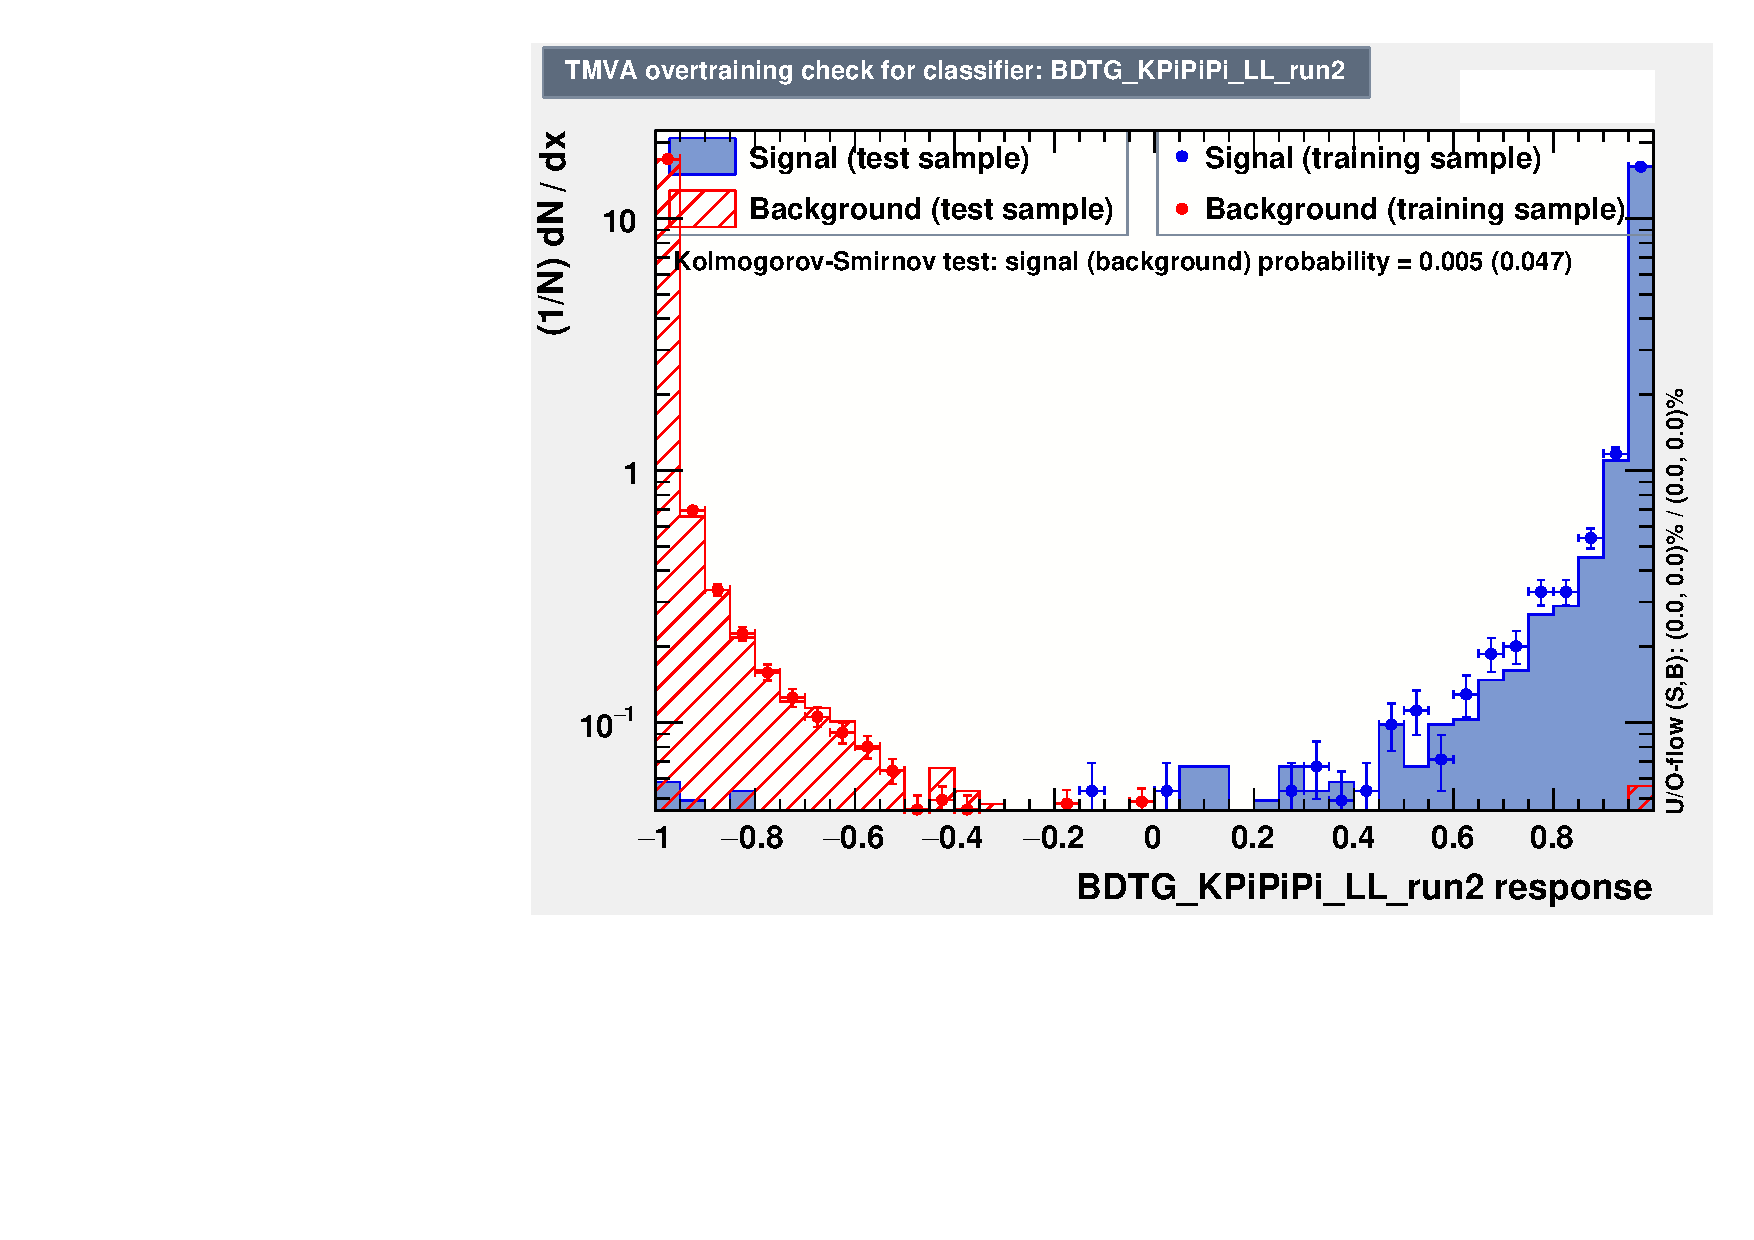
\includegraphics[width=0.5\linewidth]{figures/selection/overtraining_KPiPiPi_LL_run2.pdf}
%\put(-150,100) {(c)}
%\hfill
%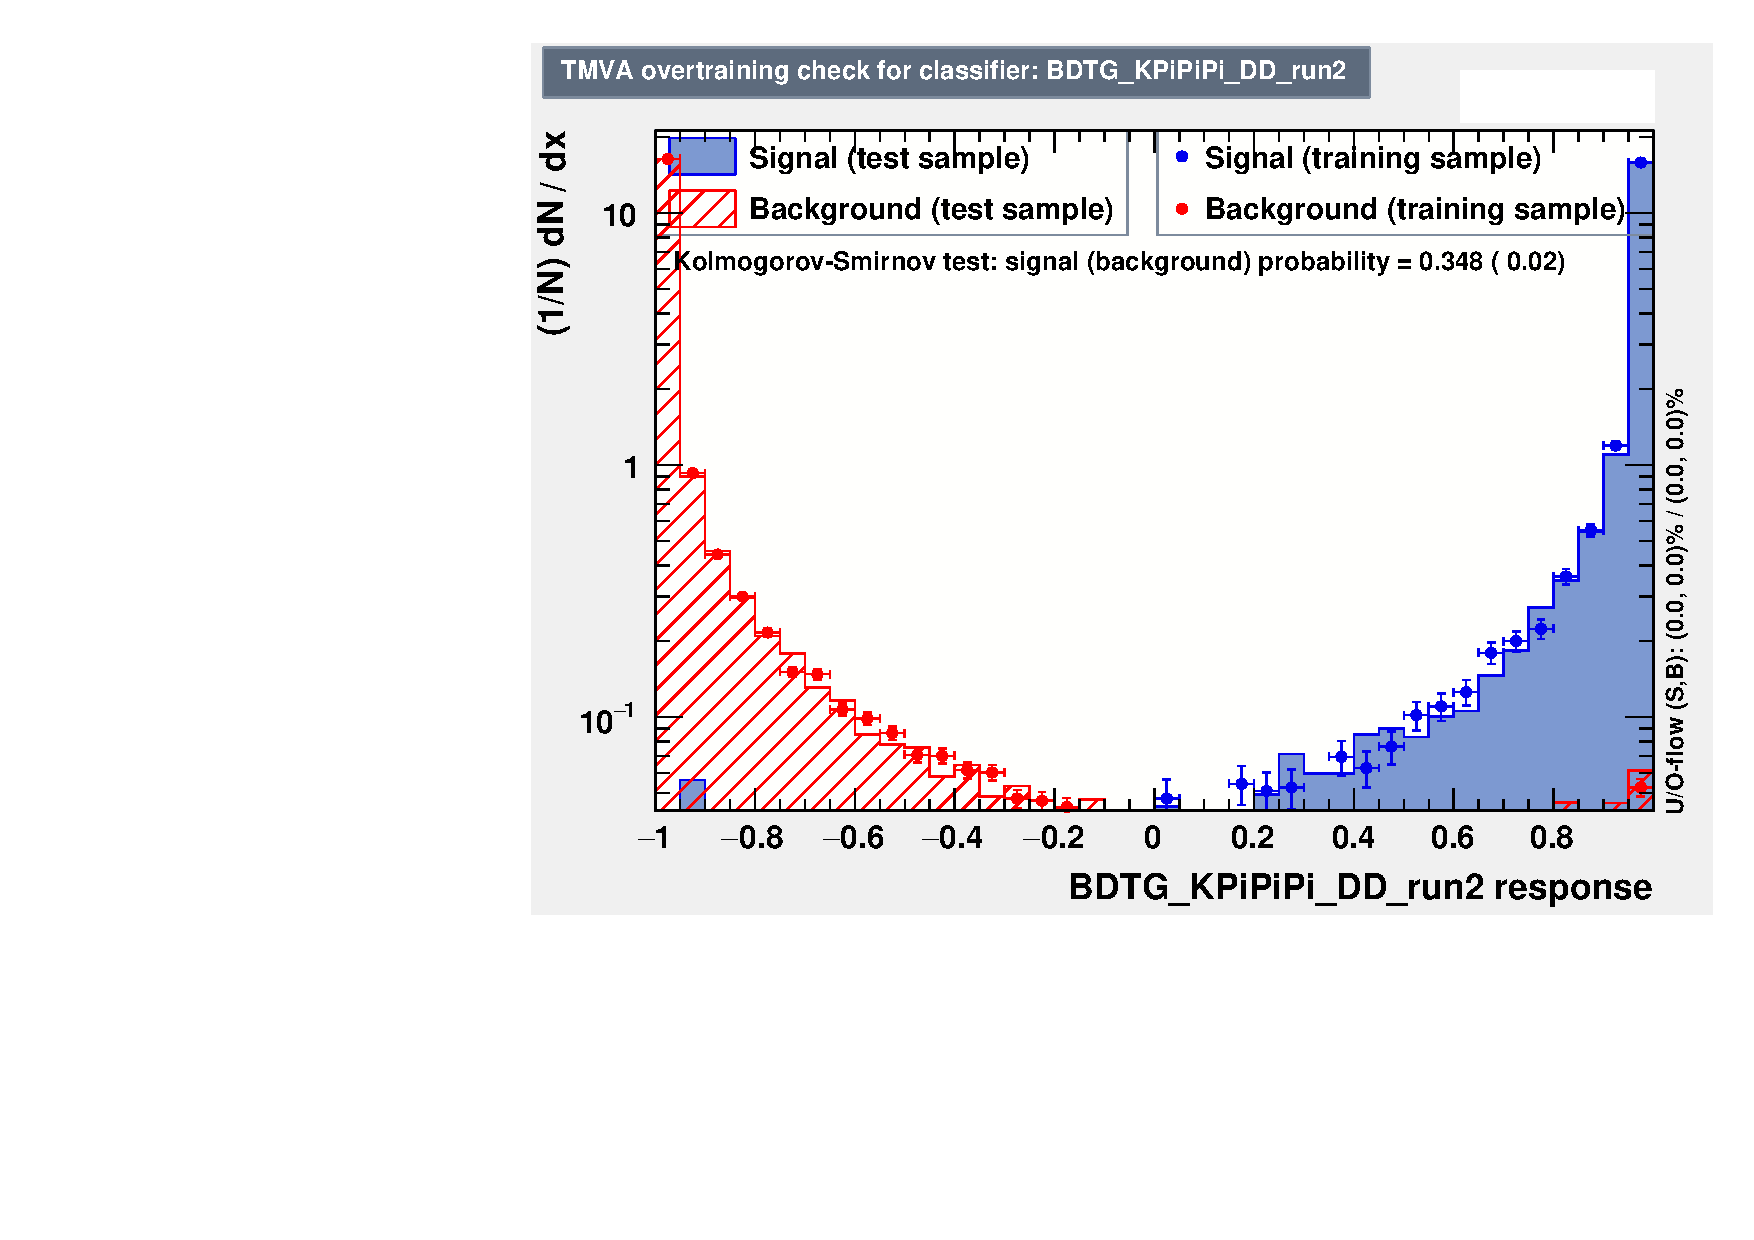
\includegraphics[width=0.5\linewidth]{figures/selection/overtraining_KPiPiPi_DD_run2.pdf}
%\put(-140,100) {(d)}
%\caption{Training and test distributions from TMVA for (a) 2-body BDT\_LL, (b) 2-body BDT\_DD, (c) 4-body BDT\_LL and (d) 4-body BDT\_DD}
%\label{BDTovertraining}
%\end{figure}

Other selection strategies were explored, including developing a series of BDTs designed to discriminate between different aspects of the signal decay. This was implemented by training and applying a \KS BDT and a \Dz BDT followed by a \Bm BDT, designed to select true \KS, \Dz and \B candidates respectively. Two approaches were tried: one using the same set of variables in all three BDTs and an alternative method using variables relating to the \KS in the BDT designed to identify true \KS mesons and variables relating to the \Dz in the BDT designed to select true \Dz mesons. Both of these methods were found to have little or no improvement on the single BDT described in this section. Many other input variables were considered for the BDT, including kinematic variables of the \Bm and \Dz mesons. These were found to give no significant improvement in BDT performance. A two-body BDT trained on \runtwo data and simulation was trained and applied to \runtwo data, which did not result in any improvement in performance compared to the BDT trained on \runone. Therefore, it was not considered necessary to have two different BDTs trained separately for \runone and \runtwo.

\subsubsection{Performance of the multivariate algoritm and choice of working point}

%The results obtained from training are applied to the testing sample in order to check for overtraining, which occurs when the classifier has learned statistical fluctuations present in the training sample. The results are shown in Figure \ref{BDTovertraining}. The training and testing distributions are in reasonable agreement, showing that the BDT is safe from overtraining effects.

The BDT selections, in conjuction with the \Kstarm mass window and \KS helicity angle, were optimised to reduce the fit error on the \CP observables, as detailed in Section \ref{sec:cpfit:optimisation}. Many pseudo-experiments were performed to calculate the fit uncertainty for each selection. To optimise the selection for the two-body GLW modes, the fit error was minimised for \Akk, \Rkk, \Apipi and \Rpipi. The BDT selection for the ADS modes was optimised to minimise the fit errors in \Rptwo and \Rmtwo. In cases when the figure of merits in these optimisation studies were not especially sensitive to changes in the selection, the selection giving the highest coherence factor, $\kappa$, i.e most stringent requirement on the \Kstarm, was chosen and the BDT signal and background efficiencies were taken into account.

After performing the optimisation, a BDT selection of 0.6 is chosen for BDT\_LL and 0.7 for BDT\_DD for all the two-body \D modes except the ADS mode. The ADS mode BDT selection is chosen to be 0.6 for BDT\_LL and 0.9 for BDT\_DD. This tighter BDT selection is justified in Section \ref{sec:cpfit:optimisation}. Averaged across the whole dataset used for the analysis, the BDT selection applied to the favoured \kpi channel gives a signal efficiency of 95\% (90\%) and a background rejection of 94\% (95\%) for LL (DD) candidates. 

For the four-body modes the same optimisation point was chosen 0.6 for BDT\_LL and 0.7 for BDT\_DD for the \decay{\Dz}{\Kp\pim\pip\pim} \decay{\Dz}{\pi\pi\pi\pi} mode, and 0.6 for BDT\_LL and 0.9 for BDT\_DD for the \decay{\Dz}{\Kp\pim\pip\pim} mode. The optimisation point was verified by minimising the fit error in psseudo-experiments for $A_{K\pi\pi\pi}$, $R^+_{K\pi\pi\pi}$ and $R^-_{K\pi\pi\pi}$. Averaged across the whole dataset, the four-body favoured \kpipipi channel gives a signal efficiency of 95\% (93\%) and a background rejection of 96\% (97\%) for LL (DD) candidates.


\subsection{Further selection requirements}

Some other selection requirements are implemented to isolate the signal candidates and tackle certain backgrounds. The different backgrounds and the strategies employed to deal with them are discussed in detail in Section \ref{sec:backgrounds}, but the resulting selection requirements are listed below:

\begin{itemize}
\item The reconstructed \Dz mass must lie within 25 \mev of the known \Dz mass
\item The reconstructed \Kstarm mass must lie within 75 \mev of the known \Kstarm mass
\item{The absolute value of $\cos(\theta_{\KS})$ must be greater than 0.3, where $\theta_{\KS}$ is defined as the angle between the \KS and the bachelor pion in the \Kstarm rest frame. This is required to reduce the non-resonant \decay{\Bm}{\D\KS\pim} background, discussed in Section \ref{sec:backgrounds:non-resonant}. }
\item{\Dz flight distance (FD) significance $>$ 2 is required to remove charmless backgrounds, discussed in Section \ref{sec:backgrounds:charmless}. The FD significance of a particle $X$ is defined as, 
\begin{equation}
\text{FD significance} = \frac{z_X - z_B}{\sqrt{\sigma_X^2 + \sigma_B^2}}
\label{FDdefinition}
\end{equation}
where $z_{X,B}$ is the $z$ position of the decay vertex of the $X,B$ particle and $\sigma_{X,B}$ is the uncertainty in the $z$ position of the $X,B$ decay vertex.}
\item{\KS flight distance significance $>$ 5 (for LL candidates only) is required to remove $B \to D\pi\pi\pi$ background, discussed in Section \ref{sec:backgrounds:b2dpipipi}. The \KS FD significance is defined by Equation \ref{FDdefinition}.}
\item{The magnitute of the difference between $\Dz_{swapped}$ and $\Dz_{PDG}$ must be greater than 15\mev for the ADS modes, where $\Dz_{swapped}$ is the reconstructed \Dz mass with the kaon reconstructed as a pion and that same pion reconstructed as a kaon, i.e. with both daughter mass hypotheses are swapped, and $\Dz_{PDG}$ is the known \Dz mass taken from the PDG. This selection criteria, known as the \Dz double misidentification veto, is applied to remove favoured \kpi events occuring in the ADS mode due to both \Dz daughters being incorrectly identified. For four-body \Dz decays, there are two possible pions that could be incorrectly reconstructed as a kaon, therefore two \Dz double misidentification vetos are applied. This background is discussed further in Section \ref{sec:backgrounds:crossfeed}.}
\end{itemize}

%Backgrounds that involve the same final state, but not via one of the intermediate state particles can also be problematic, as they would peak in the \Bm mass signal region.  backgrounds need to be reduced to negligible levels such that they do noTheset incorrectly contribute to the estimate of the signal yield. These backgrounds include decays that do not proceed via a \D meson, \decay{\Bm}{hh\Kstarm} and \decay{\Bm}{hhhh\Kstarm}, which are termed charmless decays and decays that do not proceed via a \KS meson, \decay{\Bm}{\D\pim\pip\pim}.

\subsection{Studies of peaking backgrounds}
\label{sec:backgrounds}

There are many backgrounds to be considered where certain particles in the decay chain are missed in the reconstruction process, or incorrectly identified. These effects can result in backgrounds that form peaking stuctures in the \Bm mass spectrum, which are dangerous if they significantly affect the \Bm mass spectrum. These backgrounds must either be reduced to negligible levels using targeted selection choices, or correctly modelled and included in the fit to the invariant \Bm mass spectrum. This section discusses each of the peaking backgrounds individually and the strategy employed to deal with them.

\subsubsection{Partially reconstructed \boldmath$B \to D^*K^*$ decays}
\label{sec:backgrounds:partreco}

The main class of backgrounds in this analysis is the partially reconstructed \decay{\B}{\Dstar\Kstar} decays, including \decay{\Bm}{(\decay{\Dstarz}{\Dz[\piz]})\Kstarm}, \decay{\Bm}{(\decay{\Dstarz}{\Dz[\gamma]})\Kstarm} and \decay{\Bd}{(\decay{\Dstarp}{\Dz[\pip]})\Kstarm}, where the particle in square brackets in not reconstructed. As each of these backgrounds involved a pion or photon being missed in the reconstruction, the reconstructed \Bm mass for these backgrounds appears below the signal peak. These partially reconstructed backgrounds are modelled and included as a compenent in the fit to the \Bm mass spectrum, which is discussed in detail in Section \ref{sec:massfit:partreco}.

\subsubsection{Charmless backgrounds \boldmath$B \to K^*hh$}
\label{sec:backgrounds:charmless}

Backgrounds that involve the same final state particles, but do not proceed via one of the intermediate state particles are very important, as they would peak in the same region of \Bm mass as the signal. These backgrounds need to be properly understood and reduced to negligible levels such that they do not incorrectly contribute to the estimate of the signal yield. 

Charmless backgrounds are classified as \Bm meson decays that do not proceed via a \Dz meson. This is a peaking background under the signal region which is expected to be uniform in \Dz mass. The variable used to investigate this background is the flight distance significance of the \Dz in the $z$ direction, which is defined in \eqn\ref{FDdefinition}. By requiring the \Dz to have a larger FD siginificance, it ensures that the \Dz meson is present in the decay. The charmless background is estimated by taking the \Dz mass sidebands ($>$ 50 MeV from nominal \Dz mass) in data and performing a simple fit to the invariant \B mass distribution using a Gaussian and an exponential shape. The use of DTF variables in the selection favours events towards the true \Dz mass, which would cause the charmless background to be underestimated. Therefore, in order to correctly estimate the background contribution in the \Dz mass sidebands, a modified selection is applied with the DTF vertex \chisq replaced with the vertex \chisq with no refit applied. For each \Dz decay mode, two fits are performed on data requiring the \Dz FD significance to be greater than zero and 2$\sigma$, as shown in Figure \ref{charmlesspipi} for \pipi.

\begin{figure}
\centering
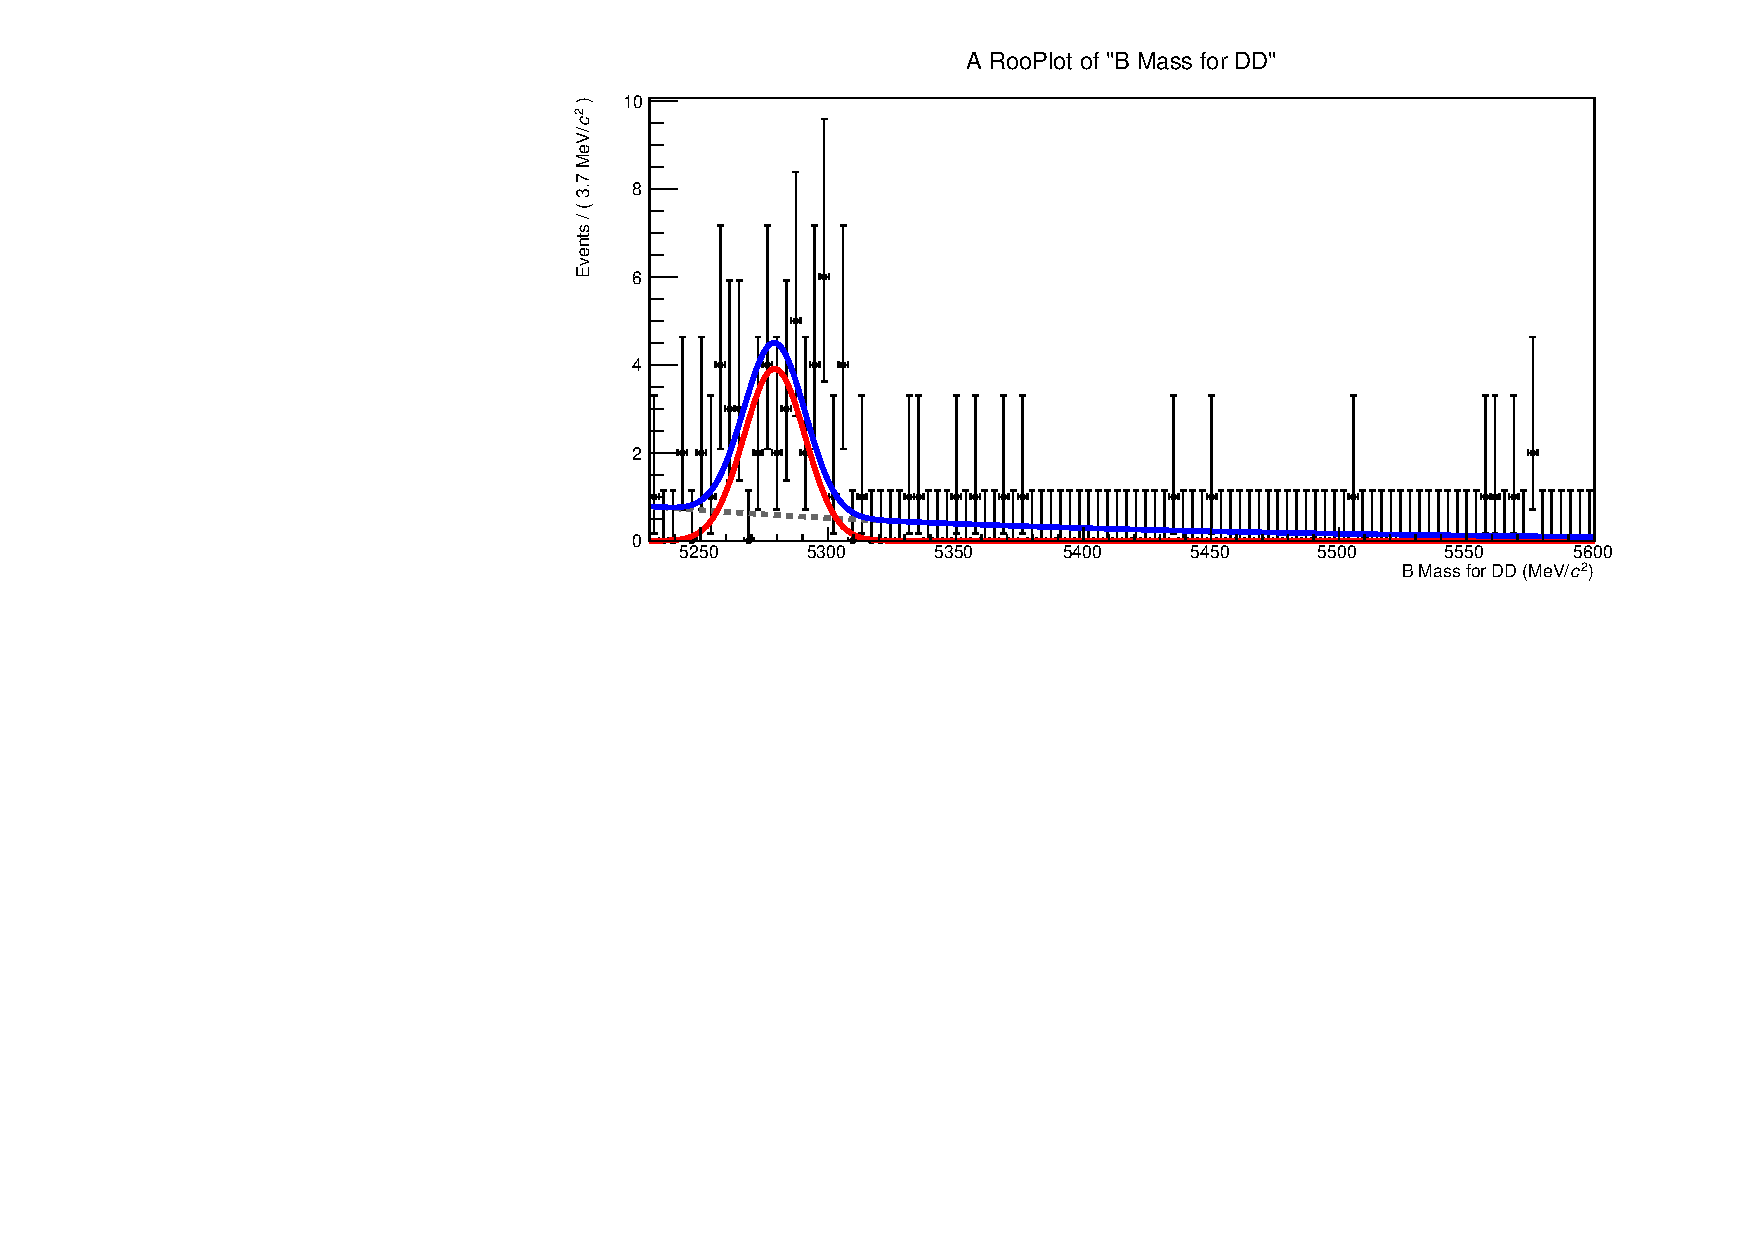
\includegraphics[width=0.7\linewidth]{figures/backgrounds/charmlessFit_PiPi_DD_FD0.pdf}
\put(-100,100) {(a)}
\hfill
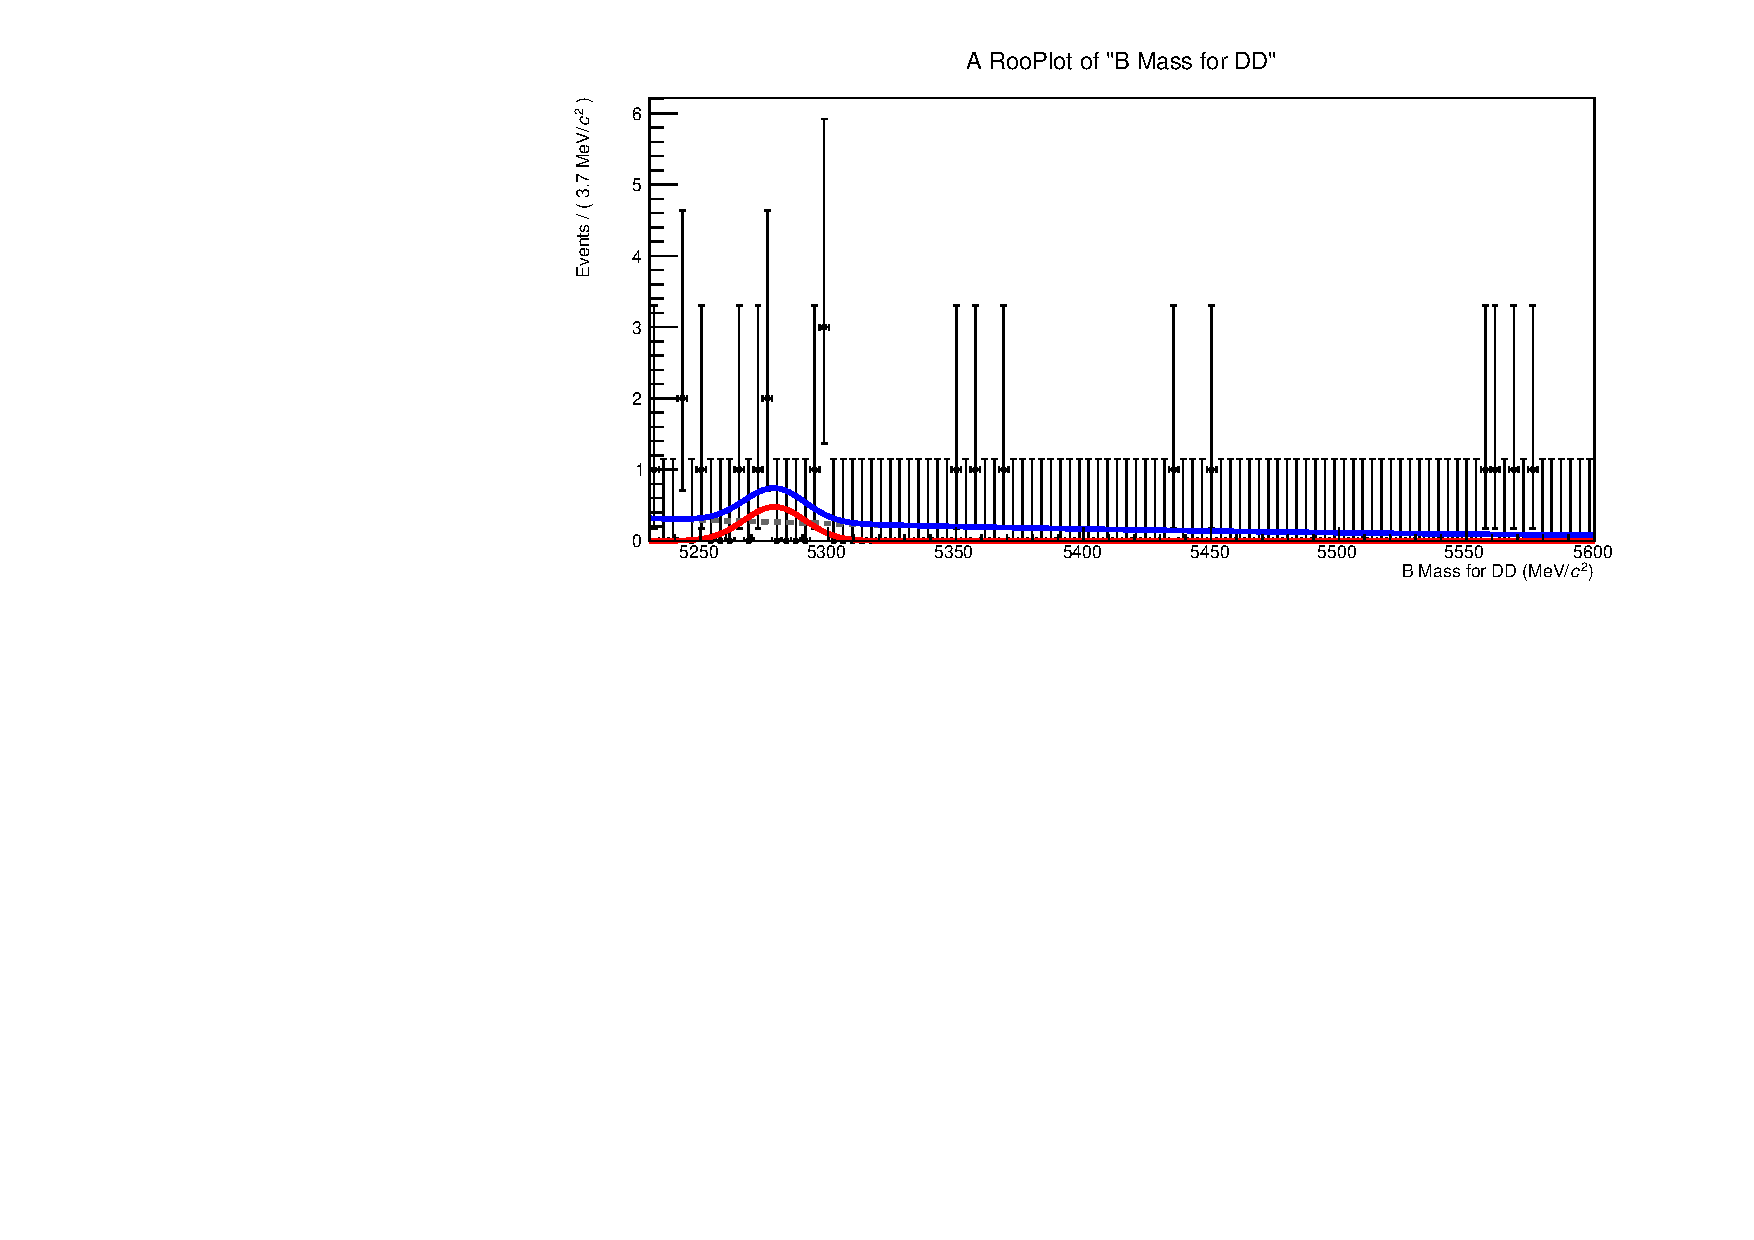
\includegraphics[width=0.7\linewidth]{figures/backgrounds/charmlessFit_PiPi_DD_FD2.pdf}
\put(-100,100) {(b)}
\caption{Fits, using the Run 1 data, to the refitted B mass taking \pipi candidates from the \Dz mass sidebands after requiring the FD significance to be (a) greater than 0 and (b) greater than 2$\sigma$. A Gaussian is used to model the signal and an exponential for the combinatoric background.}
\label{charmlesspipi}
\end{figure}

These fits give the yield of the \Bm mass peak in the \Dz mass sidebands, which are subsequently scaled to provide an estimate for this background within the \Dz mass window. By being able to quantify the number of charmless events expected in the \Bm mass spectrum after a given selection, it is possible to remove the charmless background. 
%The resulting yields estimates from fits to Run 1 data are shown in Tables \ref{charmlessyieldsnofd} and \ref{charmlessyields}, requiring the FD significance to be greater than zero and 2$\sigma$ respectively. The same fits were peformed on Run 2 data and the results for the estimated charmless contribution are given in Tables \ref{charmlessyieldsnofdRun2} and \ref{charmlessyieldsRun2}.

%\begin{table}[h] 
%\centering 
%\begin{tabular}{lll} 
%\hline 
%Mode & LL & DD \\ 
%\hline 
%$K\pi$ & $2.8 \pm 1.6$ & $2.6 \pm 1.9$ \\ 
%$KK$ & $1.2 \pm 2.0$ & $0.6 \pm 2.2$ \\ 
%$\pi\pi$ & $4.1 \pm 2.5$ & $16 \pm 4$ \\ 
%$\pi K$ & $2.0 \pm 1.3$ & $0.0 \pm 0.6$ \\ 
%$K\pi\pi\pi$ & $1.4 \pm 1.2$ & $1.5 \pm 2.0$ \\ 
%$\pi\pi\pi\pi$ & $2.2 \pm 2.4$ & $6.8 \pm 3.5$ \\ 
%$\pi K \pi\pi$ & $1.1 \pm 0.9$ & $1.3 \pm 1.2$ \\ 
%\hline 
%\end{tabular}
%\caption{Estimated charmless contribution in Run 1 data for each of the \Dz decay modes requiring the FD significance to be greater than zero.} 
%\label{charmlessyieldsnofd} 
%\end{table}
%
%\begin{table}[h]
%\centering
%\begin{tabular}{lll} 
%\hline 
%Mode & LL & DD \\ 
%\hline 
%$K\pi$ & $1.7 \pm 1.0$ & $0.2 \pm 1.6$ \\ 
%$KK$ & $0.0 \pm 0.4$ & $0.0 \pm 0.4$ \\ 
%$\pi\pi$ & $1.2 \pm 1.5$ & $2.0 \pm 1.6$ \\ 
%$\pi K$ & $1.0 \pm 0.9$ & $0.0 \pm 0.3$ \\ 
%$K\pi\pi\pi$ & $1.3 \pm 1.1$ & $0.1 \pm 3.7$ \\ 
%$\pi\pi\pi\pi$ & $0.0 \pm 7.4$ & $0.0 \pm 1.2$ \\ 
%$\pi K \pi\pi$ & $0.9 \pm 0.7$ & $0.0 \pm 0.7$ \\ 
%\hline 
%\end{tabular}
%\caption{Estimated charmless contribution in Run 1 data for each of the \Dz decay modes requiring the FD significance to be greater than 2$\sigma$.}
%\label{charmlessyields}
%\end{table}
%
%\begin{table}[h] 
%\centering 
%\begin{tabular}{lll} 
%\hline 
%Mode & LL & DD \\ 
%\hline 
%$K\pi$ & $0.0 \pm 0.4$ & $0.0 \pm 1.6$ \\ 
%$KK$ & $5.2 \pm 2.6$ & $7.1 \pm 4.0$ \\ 
%$\pi\pi$ & $11 \pm 4$ & $30 \pm 5$ \\ 
%$\pi K$ & $0.2 \pm 2.8$ & $1.1 \pm 1.7$ \\ 
%$K\pi\pi\pi$ & $0.3 \pm 2.7$ & $1.6 \pm 3.3$ \\ 
%$\pi\pi\pi\pi$ & $7.0 \pm 3.4$ & $8.7 \pm 5.3$ \\ 
%$\pi K \pi\pi$ & $0.0 \pm 2.3$ & $0 \pm 17$ \\ 
%\hline 
%\end{tabular} 
%\caption{Estimated charmless contribution in Run 2 data for each of the \Dz decay modes requiring the FD significance to be greater than zero.} 
%\label{charmlessyieldsnofdRun2} 
%\end{table}
%
%\begin{table}[h] 
%\centering 
%\begin{tabular}{lll} 
%\hline 
%Mode & LL & DD \\ 
%\hline 
%$K\pi$ & $0.0 \pm 0.3$ & $0.6 \pm 1.3$ \\ 
%$KK$ & $0.0 \pm 0.3$ & $0.0 \pm 0.7$ \\ 
%$\pi\pi$ & $0.0 \pm 1.2$ & $2.3 \pm 2.2$ \\ 
%$\pi K$ & $0.4 \pm 1.0$ & $0.0 \pm 0.5$ \\ 
%$K\pi\pi\pi$ & $1.0 \pm 1.4$ & $0.0 \pm 7.6$ \\ 
%$\pi\pi\pi\pi$ & $1.4 \pm 2.3$ & $0.0 \pm 1.0$ \\ 
%$\pi K \pi\pi$ & $0.0 \pm 10.6$ & $1.4 \pm 1.5$ \\ 
%\hline 
%\end{tabular} 
%\caption{Estimated charmless contribution in Run 2 data for each of the \Dz decay modes requiring the FD significance to be greater than 2$\sigma$.} 
%\label{charmlessyieldsRun2}
%\end{table}

In the final selection, the \Dz FD significance is required to exceed 2$\sigma$, as all charmless contributions are consistent with zero under this requirement. The expected yields in the \kpi favoured and \kk modes are significantly less than 1\% of the signal yield and are therefore considered negligible. However, the estimated charmless contribution in the \pipi mode is greater than 1\% and so could affect the results, therefore the possible charmless contribution in the \pipi mode is considered as a source of systematic uncertainty, details are given in Section \ref{sec:systematics}. 

\subsubsection{\boldmath \decay{\Bm}{\D\pim\pip\pim}}
\label{sec:backgrounds:b2dpipipi}

Having considered backgrounds without the \Dz meson present, we now consider backgrounds that do not occur via a \KS meson. These \decay{\Bm}{\D\pim\pip\pim} decays, with a branching fraction of $5.7 \times 10^{-3}$~\cite{PDG2014} (about 50 times the signal \decay{\Bm}{\D\Kstarm(\KS(\pip\pim)\pim)} branching fraction), are expected to occur as a peaking background underneath the signal. In order to remove this background, events are selected with the requirement that the \KS has travelled within the detector. For DD candidates this requirement is already satisfied, however for LL candidates a minimum requirement on the flight distance significance of the \KS in the z direction, defined in Equation \ref{FDdefinition}, is used to remove this background. 

The \decay{\Bm}{\D\pim\pip\pim} background is estimated by taking the \KS mass sidebands ($>$ 20 MeV from nominal \KS mass) in data and performing a fit to the invariant \Bm mass distribution. A Gaussian is used to model the signal and an exponential for the combinatoric background. A modified selection is applied that does not use any DTF variables, as described in Section \ref{sec:backgrounds:charmless}. This fit is performed on \kpi data requiring the \KS FD significance to be greater than zero and 5$\sigma$, as shown in Figure \ref{strangelessfits}. Using these fits the estimated \decay{\B}{\D\pi\pi\pi} yield in the signal region with \KS FD significance $>$ 0 is $77 \pm 11$ and with \KS FD significance $>$ 5 is $1.0 \pm 1.0$. For the final selection, the FD significance is required to be greater than 5$\sigma$ as it removes all of the \decay{\Bm}{\D\pim\pip\pim} background.


\begin{figure}
\centering
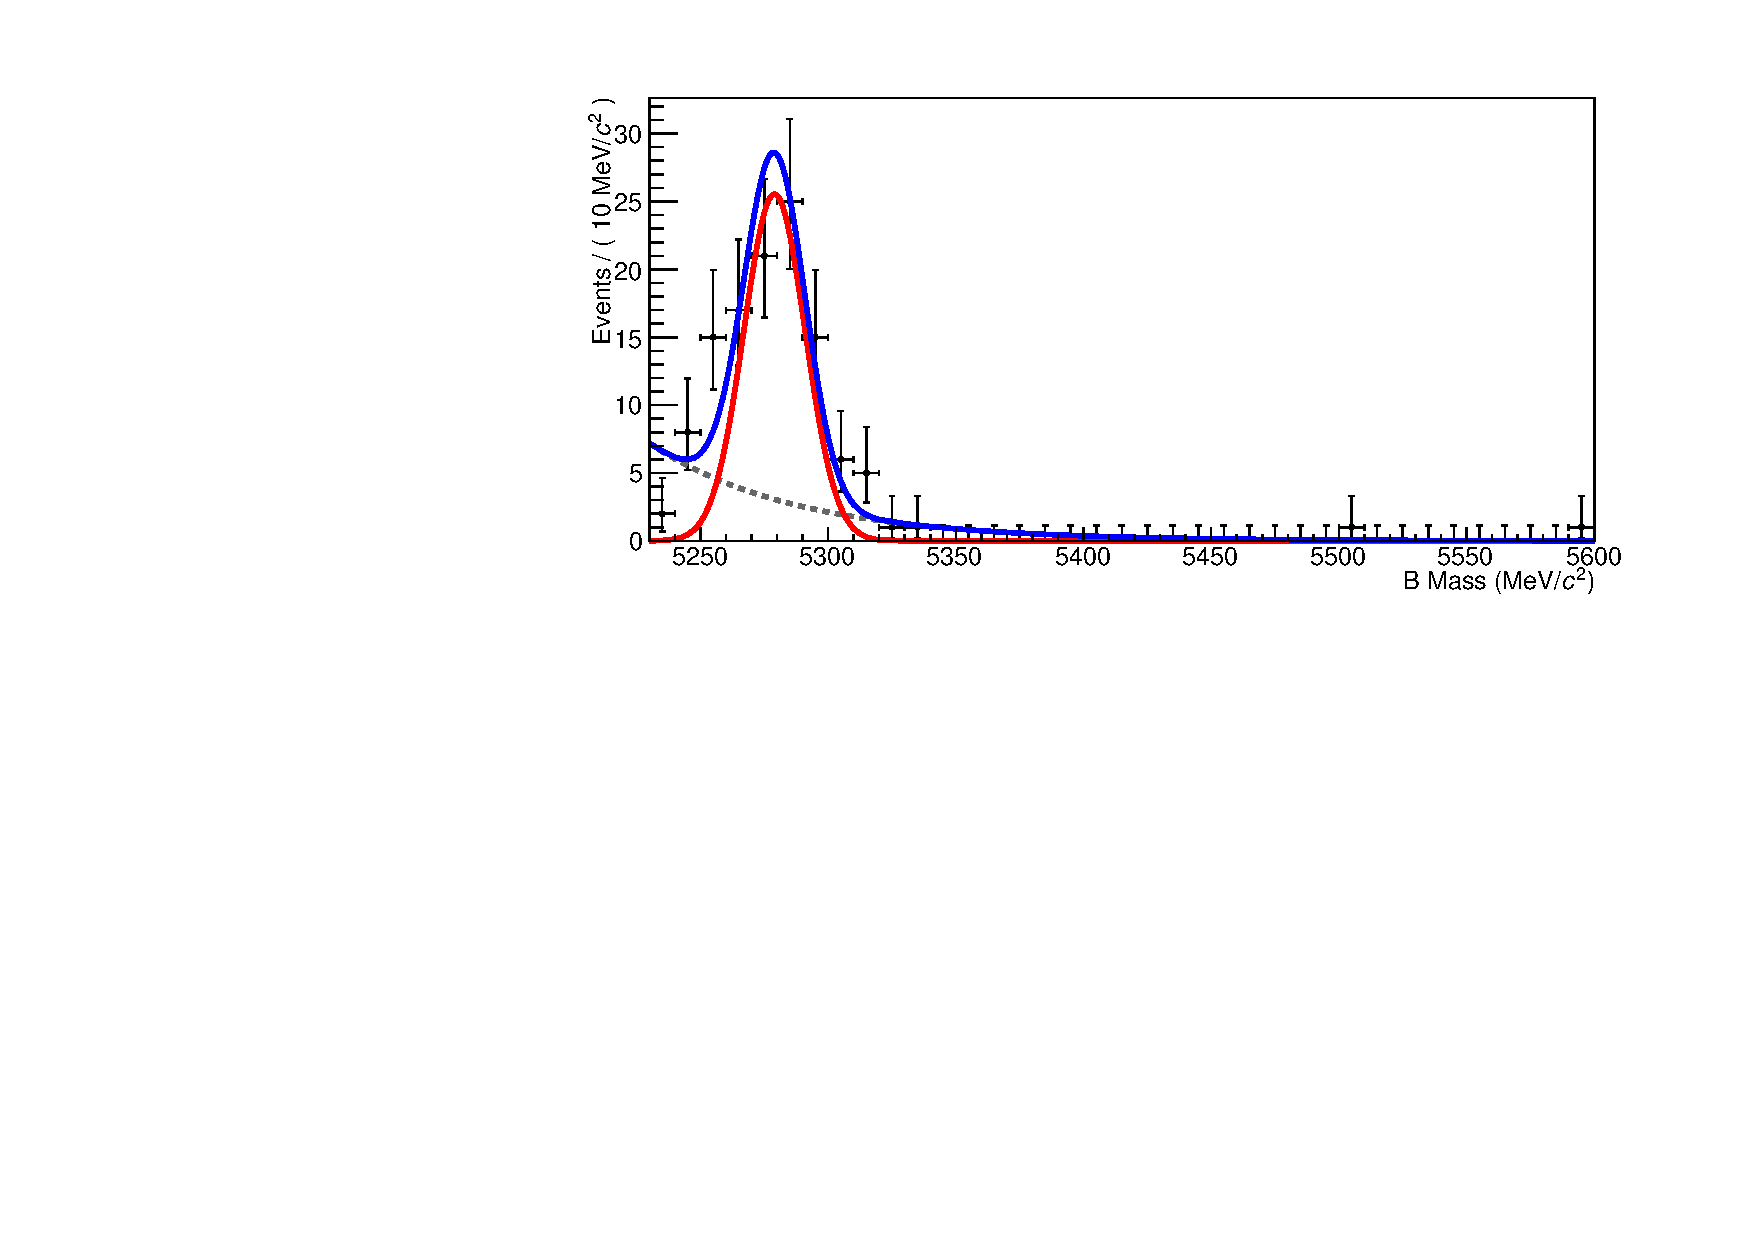
\includegraphics[width=0.7\linewidth]{figures/backgrounds/B2DpipipiFit_KPi_LL_FD0_run2.pdf}
\put(-100,100) {(a)}
\hfill
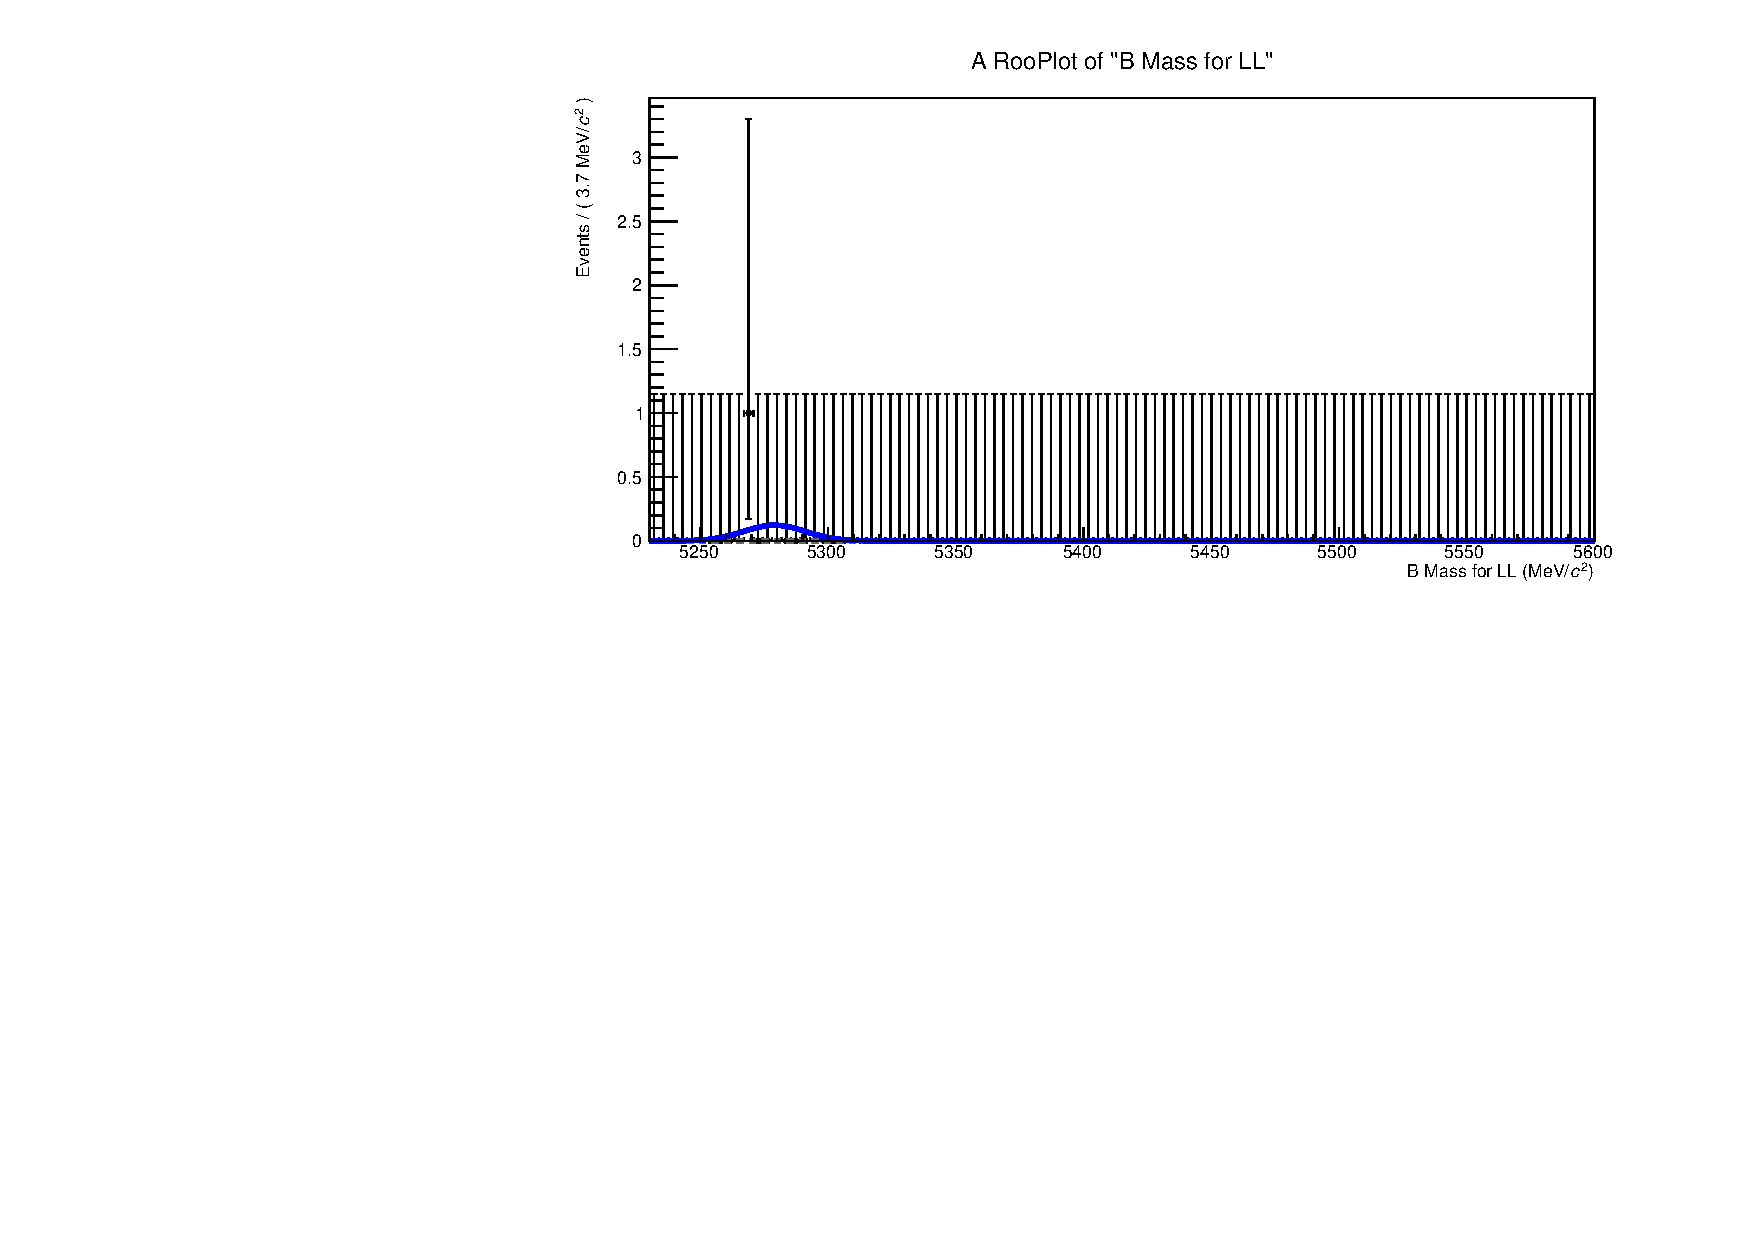
\includegraphics[width=0.7\linewidth]{figures/backgrounds/B2DpipipiFit_KPi_LL_FD5_run2.pdf}
\put(-100,100) {(b)}
\caption{Fits to the Run 2 refitted B mass taking \decay{\Dz}{\Km\pip} candidates from the \KS mass sidebands after requiring the FD significance to be (a) greater than 0 and (b) greater than 5$\sigma$.}
\label{strangelessfits}
\end{figure}

\subsubsection{Non-resonant \boldmath$B \to DK_s\pi$}
\label{sec:backgrounds:non-resonant}

The \Kstarm meson has a large natural width (about 50\mevcc~\cite{PDG2016}) therefore \decay{\Bm}{\D\KS\pim} may be non-negligible in this region, which would affect the measurement of \Pgamma. This is accounted for by the coherence factor $\kappa$, discussed in Section \ref{sec:theory:gamma}. It is necessary to optimise the selection to get maximum sensitivity to \Pgamma, which involves optimising between obtaining a high yield and a high coherence. This is achieved, firstly by only accepting \Kstarm candidates that have a reconstructed mass within 75\mevcc to the known mass and secondly by exploiting the vector properties of the signal decay. 

As the \Kstarm meson is a vector meson, the \decay{\Bm}{\D\Kstarm} decay is a Scalar $\to$ Scalar Vector decay, forcing the \Kstarm to be longitiduinally polarised. If we define the \KS helicity angle, $\theta_{\KS}$, as the angle between the \KS and the bachelor pion in the \Kstarm rest frame, $\cos(\theta_{\KS})$ for pure \decay{\Bm}{\D\Kstarm} follows a parabolic distribution, as shown in Figure \ref{helicitycut}. As \decay{\Bm}{\D\KS\pim} decays are expected to be uniformly distributed in $\cos(\theta_{\KS})$, by removing candidates that have a small absolute value of $\cos(\theta_{\KS})$ a large amount of non-resonant background can be removed while retaining almost all of the pure \decay{\Bm}{\D\Kstarm} signal. Removing events with an absolute value of $\cos(\theta_{\KS})$ less than 0.3 retains 97\% of true \decay{\Bm}{\D\Kstarm} decays, while rejecting 30\% of the non-resonant background. The optimisation of the \Kstarm mass and \KS helicity angle selection is discussed in detail in Section \ref{sec:cpfit:optimisation}.

%Non-resonant background is reduced by removing events in which the \KS\pion invariant mass is greater than 75 MeV from the nominal \Kstarpm mass. \decay{\Bpm}{\D\Kstarpm} is a Scalar $\to$ Scalar Vector decay, which means the \Kstarpm must be londitudially polarised, so the $K_s$ helicity angle of pure \D\Kstarpm events follows a $\cos^2\theta$ distribution, as shown in Figure \ref{helicitycut}, compared to the uniform distribution of non-resonant components. Removing events with an absolute value of $\cos^2\theta$ less than 0.3 improves the purity of \decay{\Bm}{\D\Kstarm} decays compared to non-resonant background.

\begin{figure}[h]
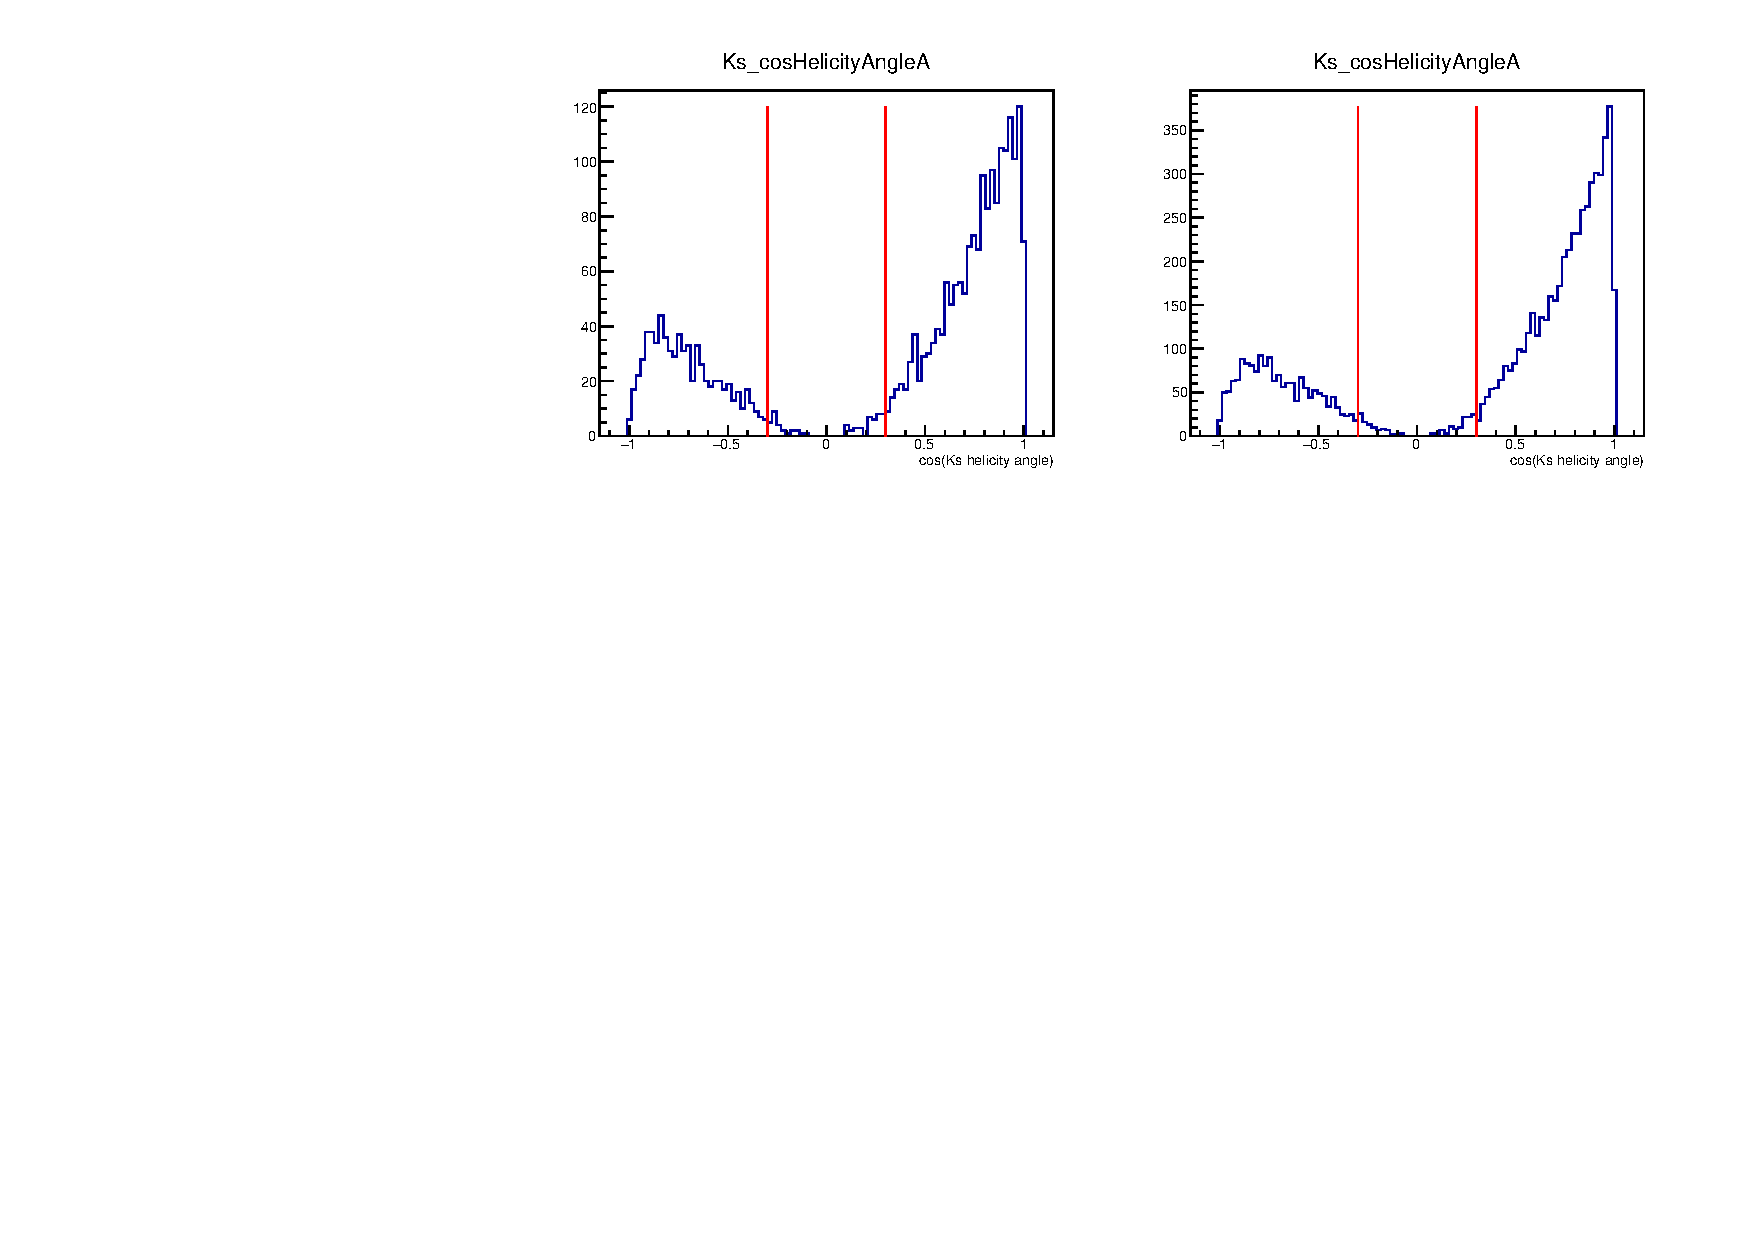
\includegraphics[width=\linewidth]{figures/backgrounds/KsHelicityCut.pdf}
\put(-380,100) {(a)}
\put(-170,100) {(b)}
\caption{Distribution of the cosine of \KS helicity angle from a simulated sample of \kpi events for (a) LL candidates and (b) DD candidates.}
\label{helicitycut}
\end{figure}

Having determined the \Kstarm selection, the value of the coherence factor, $\kappa$, is estimated and then used alongside the \CP observables to extract \Pgamma, $r_B$ and $\delta_B$. The parameter $\kappa$ is estimated by constructing an amplitude model and using this to generate many models, where the amplitudes and phases of the model components are varied; this method is detailed in Section \ref{sec:interpretation:coherence}. The resulting estimate for the value of $\kappa$ is $0.95 \pm 0.06$.

It can be observed from Figure \ref{helicitycut} that the \KS helicity angle distribution is not symmetric. Figure \ref{helictyasymmetry}(a) shows the \KS helicity angle distribution in a simulated signal sample with no generator level selection applied, which is symmetric as expected. However, Figure \ref{helictyasymmetry}(b) shows the same distrbution but with momentum, $p$, and transverse momentum, $p_T$, thresholds placed on the bachelor pion that are present in the stripping line, which reproduces the oberved asymmetry. Therefore, the asymmetry in this variable, manifest in both data and simulation, is due to the momentum and transverse momentum selections placed on the bachelor pion in the stripping line.

\begin{figure}[h]
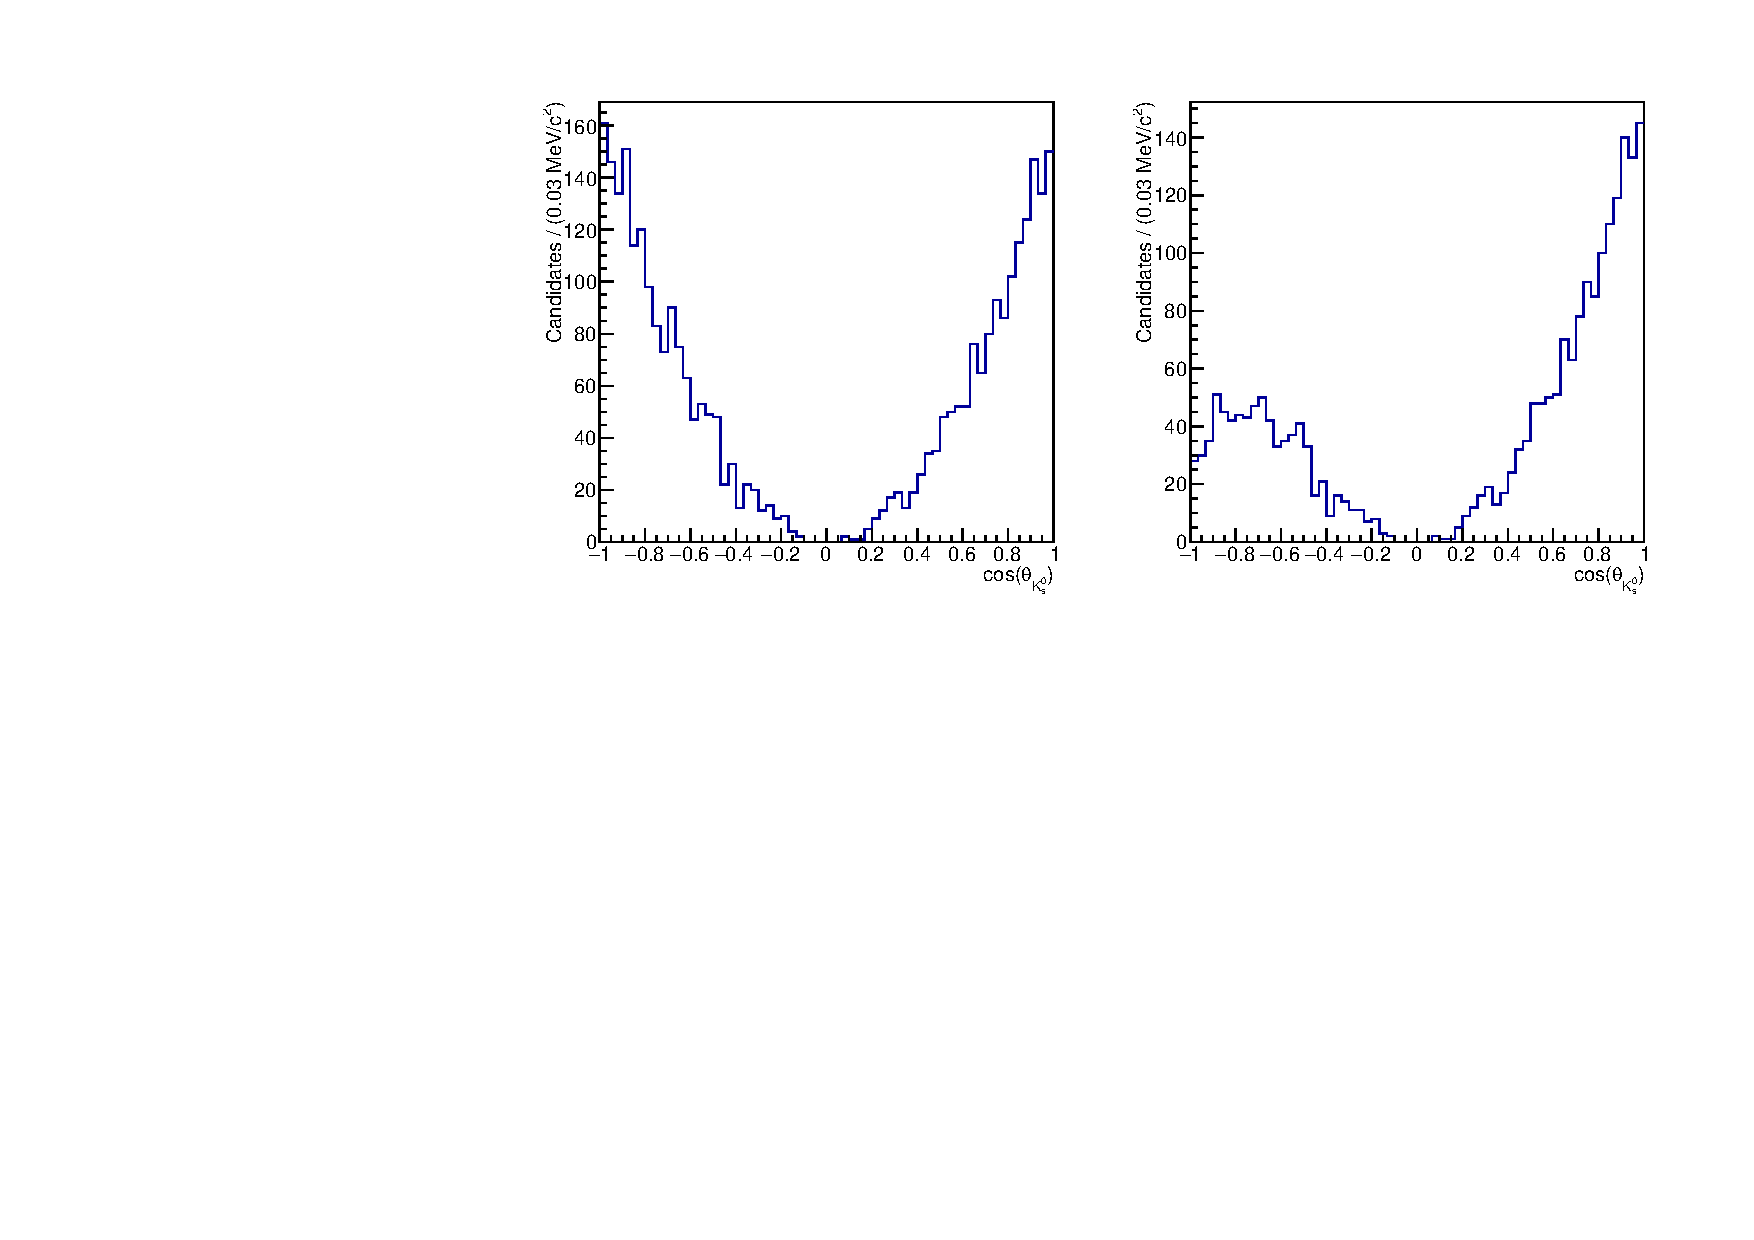
\includegraphics[width=\linewidth]{figures/helicityAngleAsymmetry.pdf}
\put(-360,150) {(a)}
\put(-150,150) {(b)}
\caption{Distribution of the cosine of \KS helicity angle from a simulated sample of \kpi events at generator level with (a) no selection applied, and (b) bachelor $p > 2500$ MeV and bachelor $p_T > 250$ MeV applied, as in the stripping line.}
\label{helictyasymmetry}
\end{figure}

%It is necessary to estimate the fraction of non-resonant \decay{\B}{\D\KS\pi} in the signal candidates. Figure \ref{kshelicitycomparison} shows a comparison of \KS helicity angle and the \KS momentum between the simulated signal sample and sWeighted data. There is a discrepancy in both \KS helicity angle distribution and the \KS momentum distribution. The discrepancy in the momentum distribution was corrrected by reweighting the simulated sample in $p_T$, the resulting helicity angle distribution is consistent with the data, as shown in Figure \ref{kshelicitycomparisonreweighted}.
%
%\begin{figure}[h]
%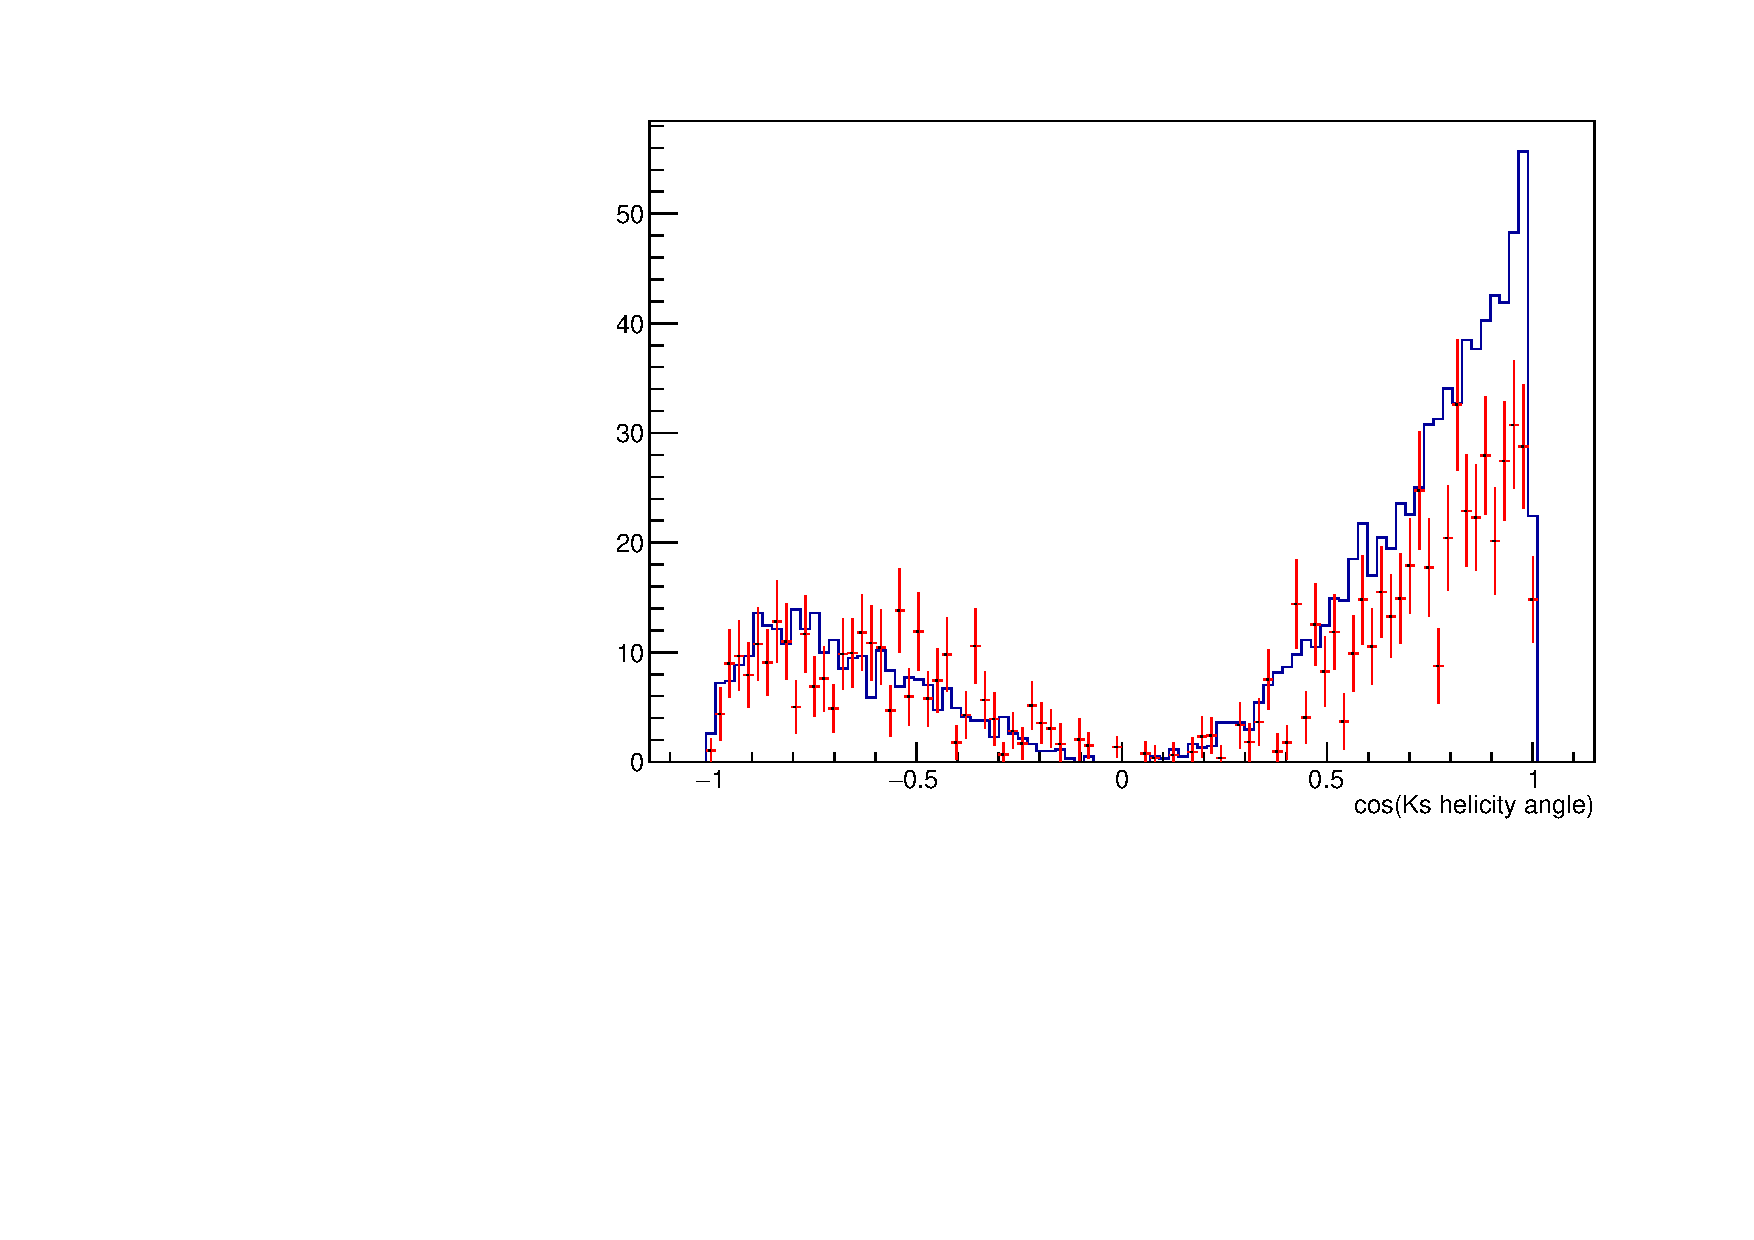
\includegraphics[width=0.5\linewidth]{figures/backgrounds/KsHelicityAngle_sweighted.pdf}
%\put(-170,100) {(a)}
%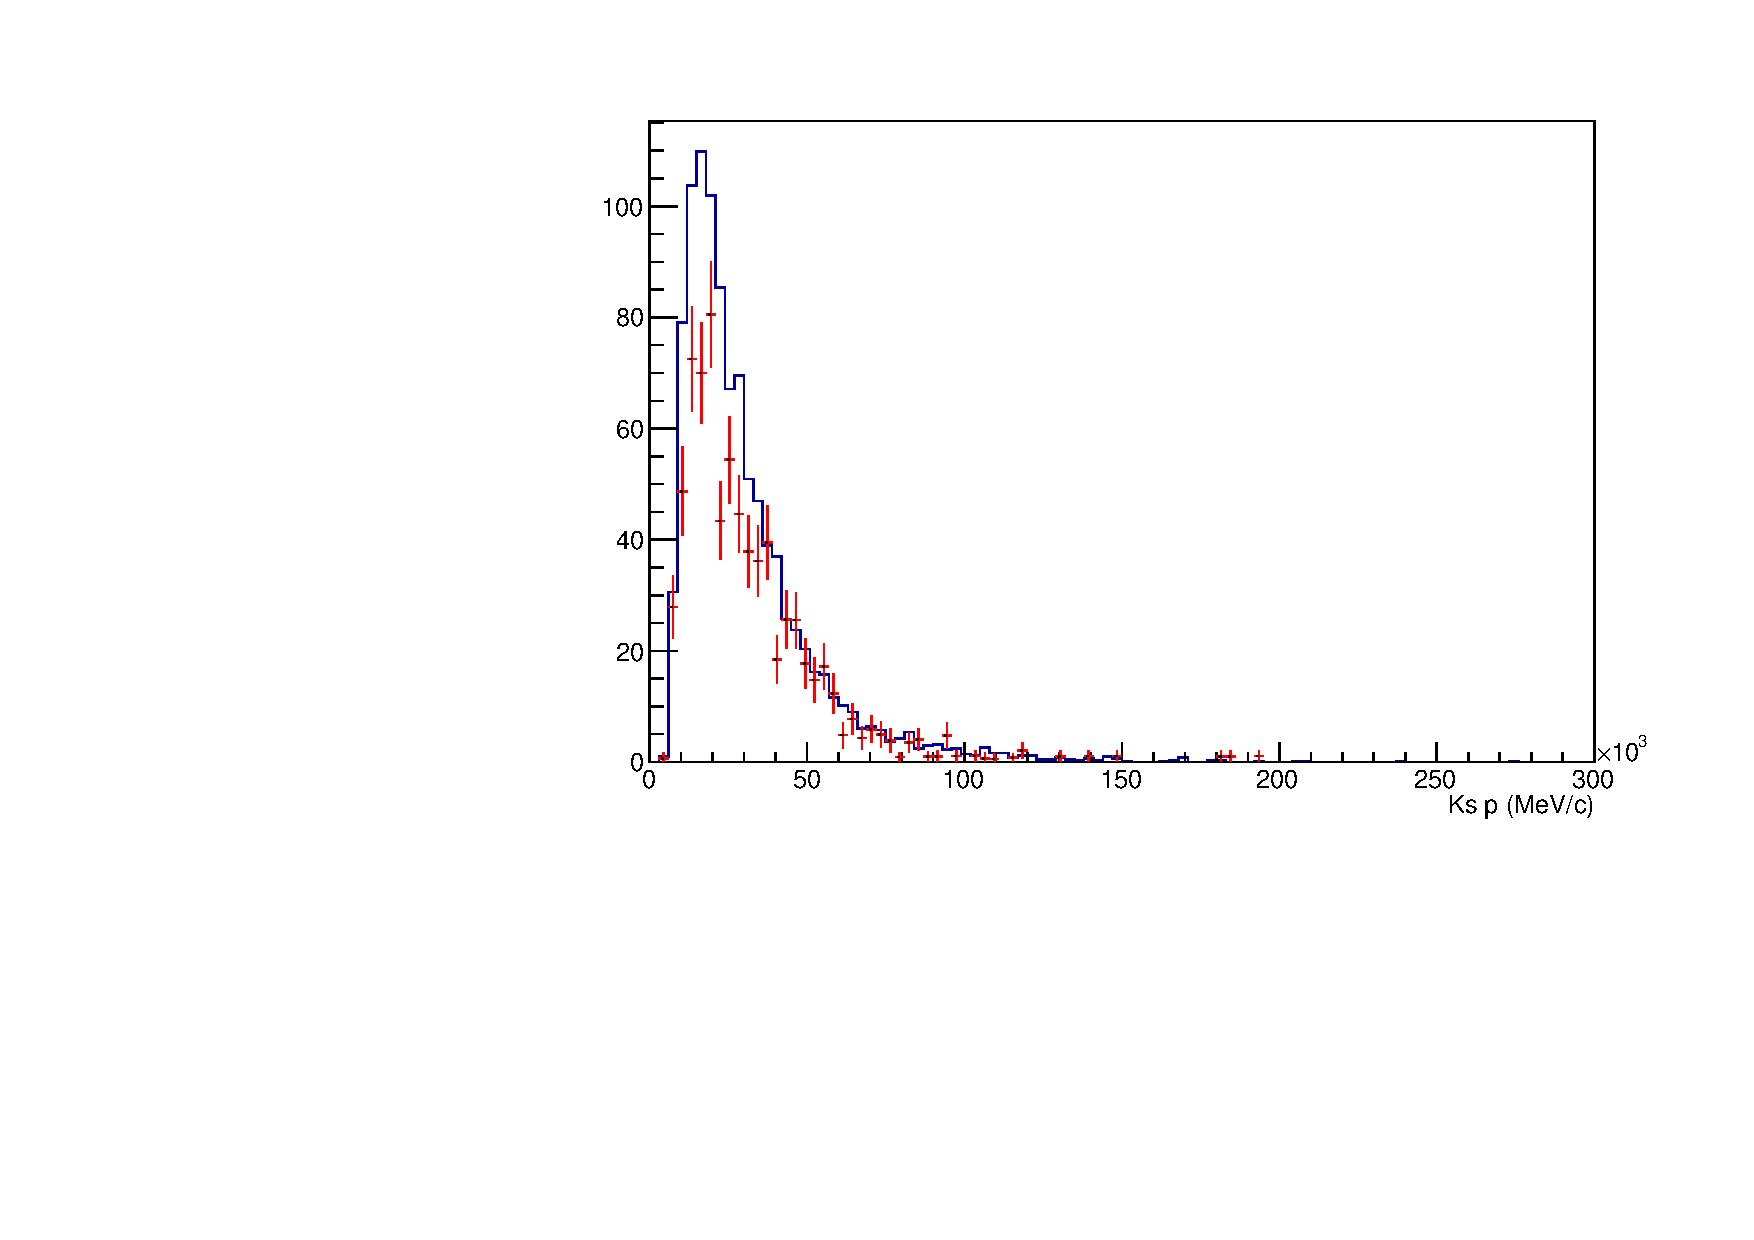
\includegraphics[width=0.5\linewidth]{figures/backgrounds/KsP_sweighted.pdf}
%\put(-170,100) {(b)}
%\caption{Comparison of (a) cosine of the helicity angle distribution and (b) the \KS momentum distribution in sWeighted data (red) and MC (blue)}
%\label{kshelicitycomparison}
%\end{figure}
%
%\begin{figure}[h]
%\centering
%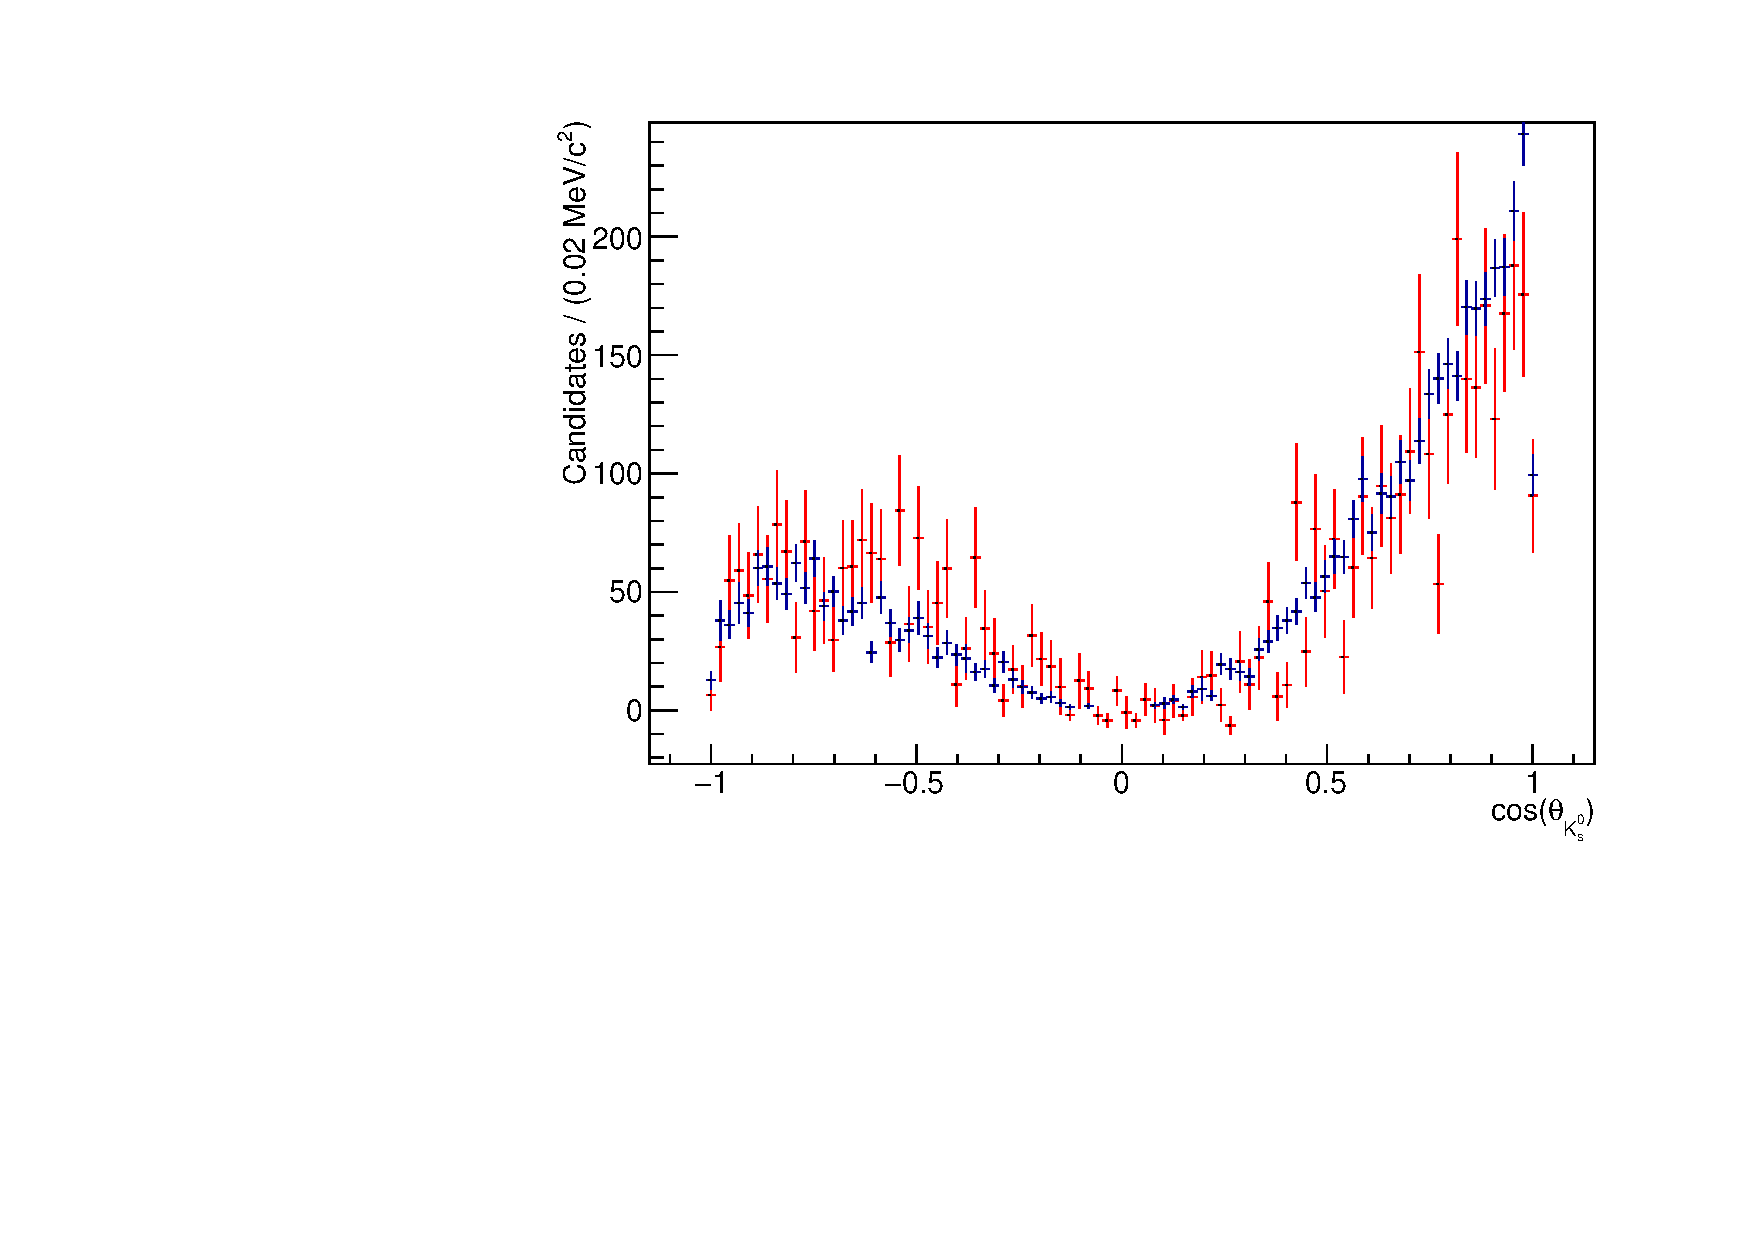
\includegraphics[width=0.6\linewidth]{figures/backgrounds/KsHelicityAngle_sweighted_MCweighted.pdf}
%\caption{Comparison of cosine of the helicity angle distribution in sWeighted data (red) and MC (blue) reweighted to give the same \KS momentum distribution}
%\label{kshelicitycomparisonreweighted}
%\end{figure}

\subsubsection{Crossfeed background}
\label{sec:backgrounds:crossfeed}

The \Bm mass spectrum for the doubly Cabibo supressed ADS mode, \pik, can contain background events coming from the favoured \kpi mode, where the \Dz daughter mass hypotheses are swapped, i.e. the kaon is misidentified as a pion and the pion is misidentified as a kaon. When considering the two-body \Dz decay modes, the favoured \kpi mode has a braching ratio 281 times higher than the \pik mode. Particle identification requirements, detailed in Section \ref{sec:selection:pid}, on the \Dz daughters significantly reduce this background, however in order to bring it down to negligible levels a veto must be applied. An alternative \Dz mass, $D_{\text{swapped}}$, is calculated where the \Dz meson is reconstructed with both daughter mass hypotheses are swapped. The veto applied requires $D_{\text{swapped}}$ to be greater than 15 MeV away from the known \Dz mass. This veto is illustrated in Figure \ref{Dmassveto}, which shows the distributions from simulated samples for DD canidates in Run 1. The veto is only applied to the \pik mode in this analysis. It is found to be 92.5\% efficient at retaining genuine signal, corresponding to events that lie within the red lines in Figure \ref{Dmassveto} (a), while only retaining 8.7\% of double misidentification background, coresponding to events that lie within the red lines in Figure \ref{Dmassveto} (b). 

For the four-body modes, the equivalent background can appear in the suppressed \pikpipi mode due to contamination from the favoured \kpipipi. There are two \pip mesons that could be misidentified as a \Kp meson, therefore in this case two vetos need to be applied. The alternative \Dz mass is reconstructed as a swapped mass hypothesis where the kaon is swapped with the lower momentum pion, $D_{\text{swapped}}^{\text{low p}}$, and the kaon is swapped with the higher momentum pion, $D_{\text{swapped}}^{\text{high p}}$. The veto is applied to both these reconstructed masses as shown in Figure \ref{Dmassveto4body}.

\begin{figure}[h]
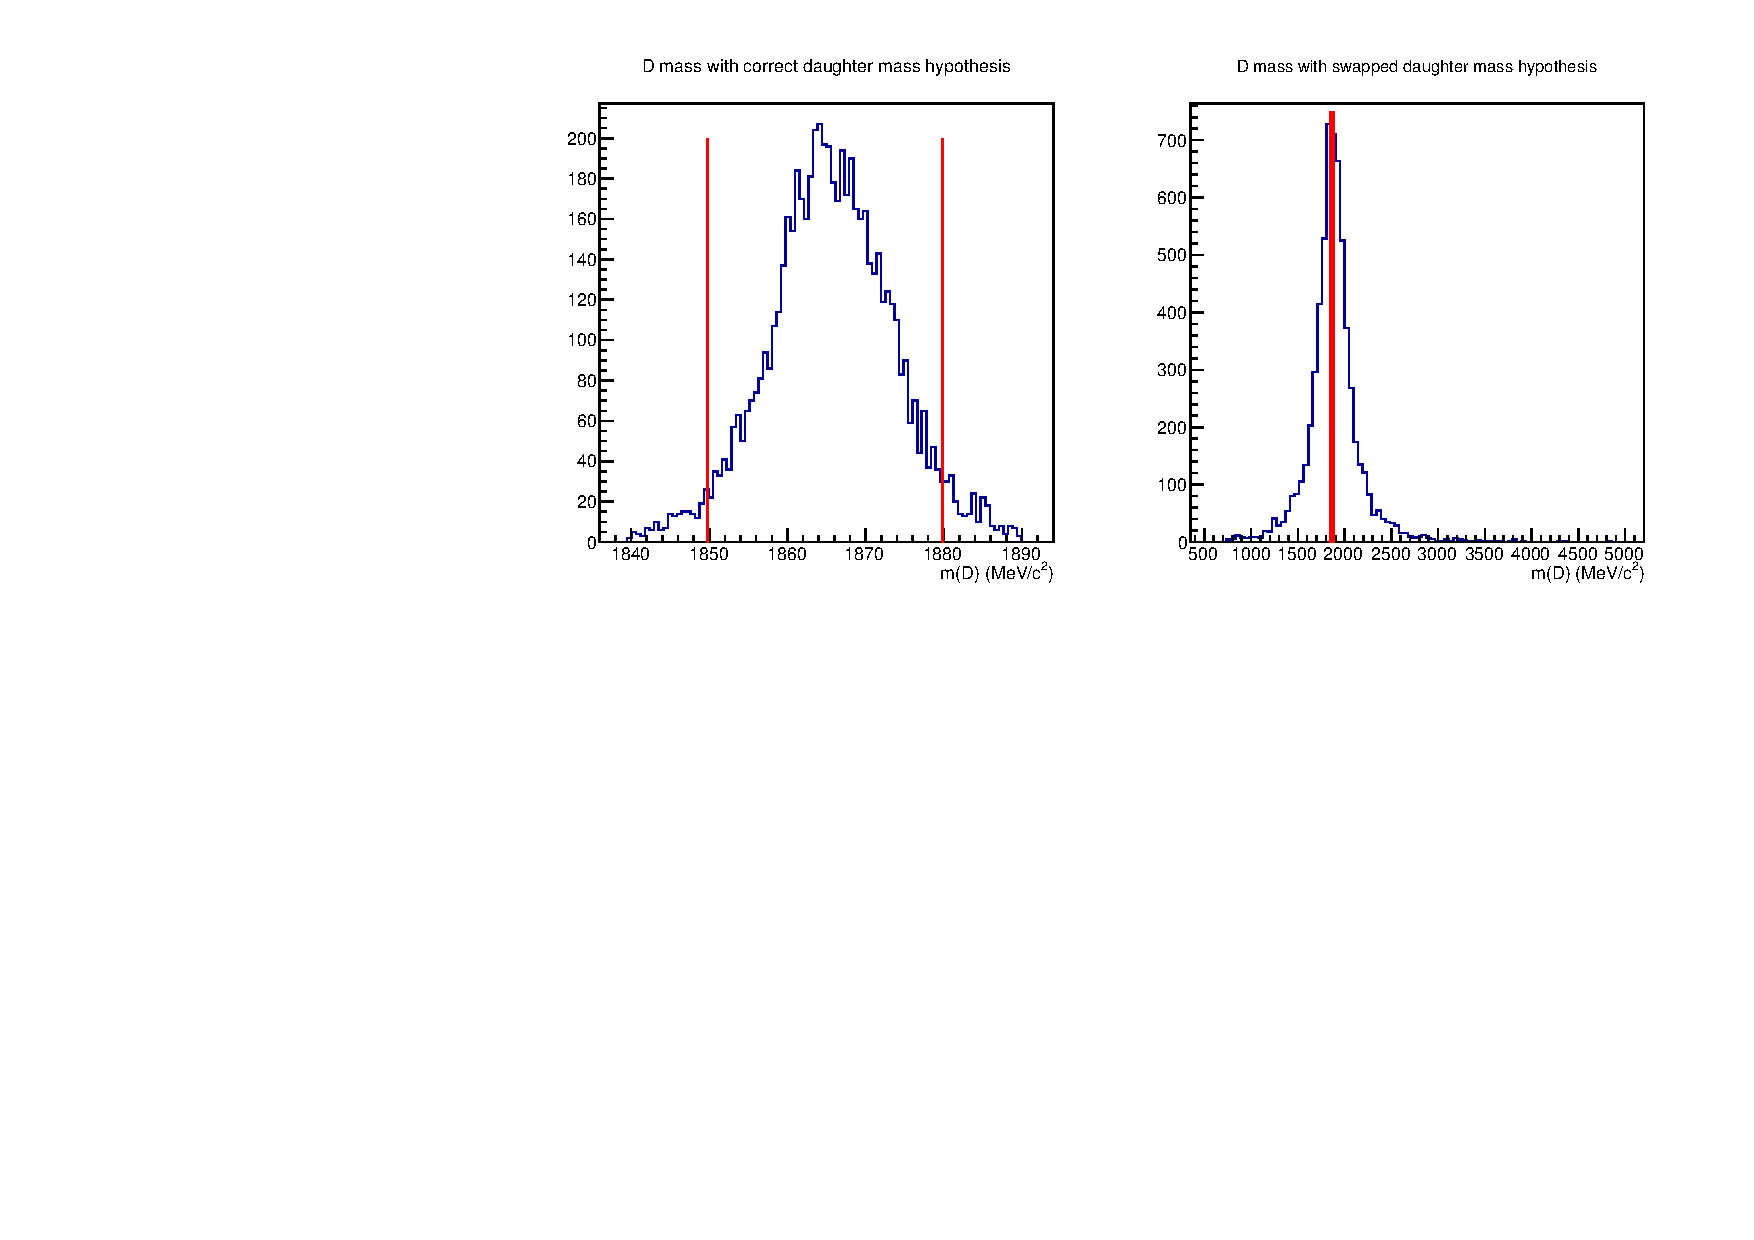
\includegraphics[width=\linewidth]{figures/backgrounds/Dmassveto.pdf}
\put(-380,150) {(a)}
\put(-170,150) {(b)}
\caption{Distributions from simulated samples for DD canidates in Run 1 showing \Dz mass with (a) the correct \Dz daughter mass hypothesis and (b) the swapped \Dz daughter mass hypothesis. The red lines correspond to the double misidentification veto selection window applied to the \pik mode.}
\label{Dmassveto}
\end{figure}

\begin{figure}[h]
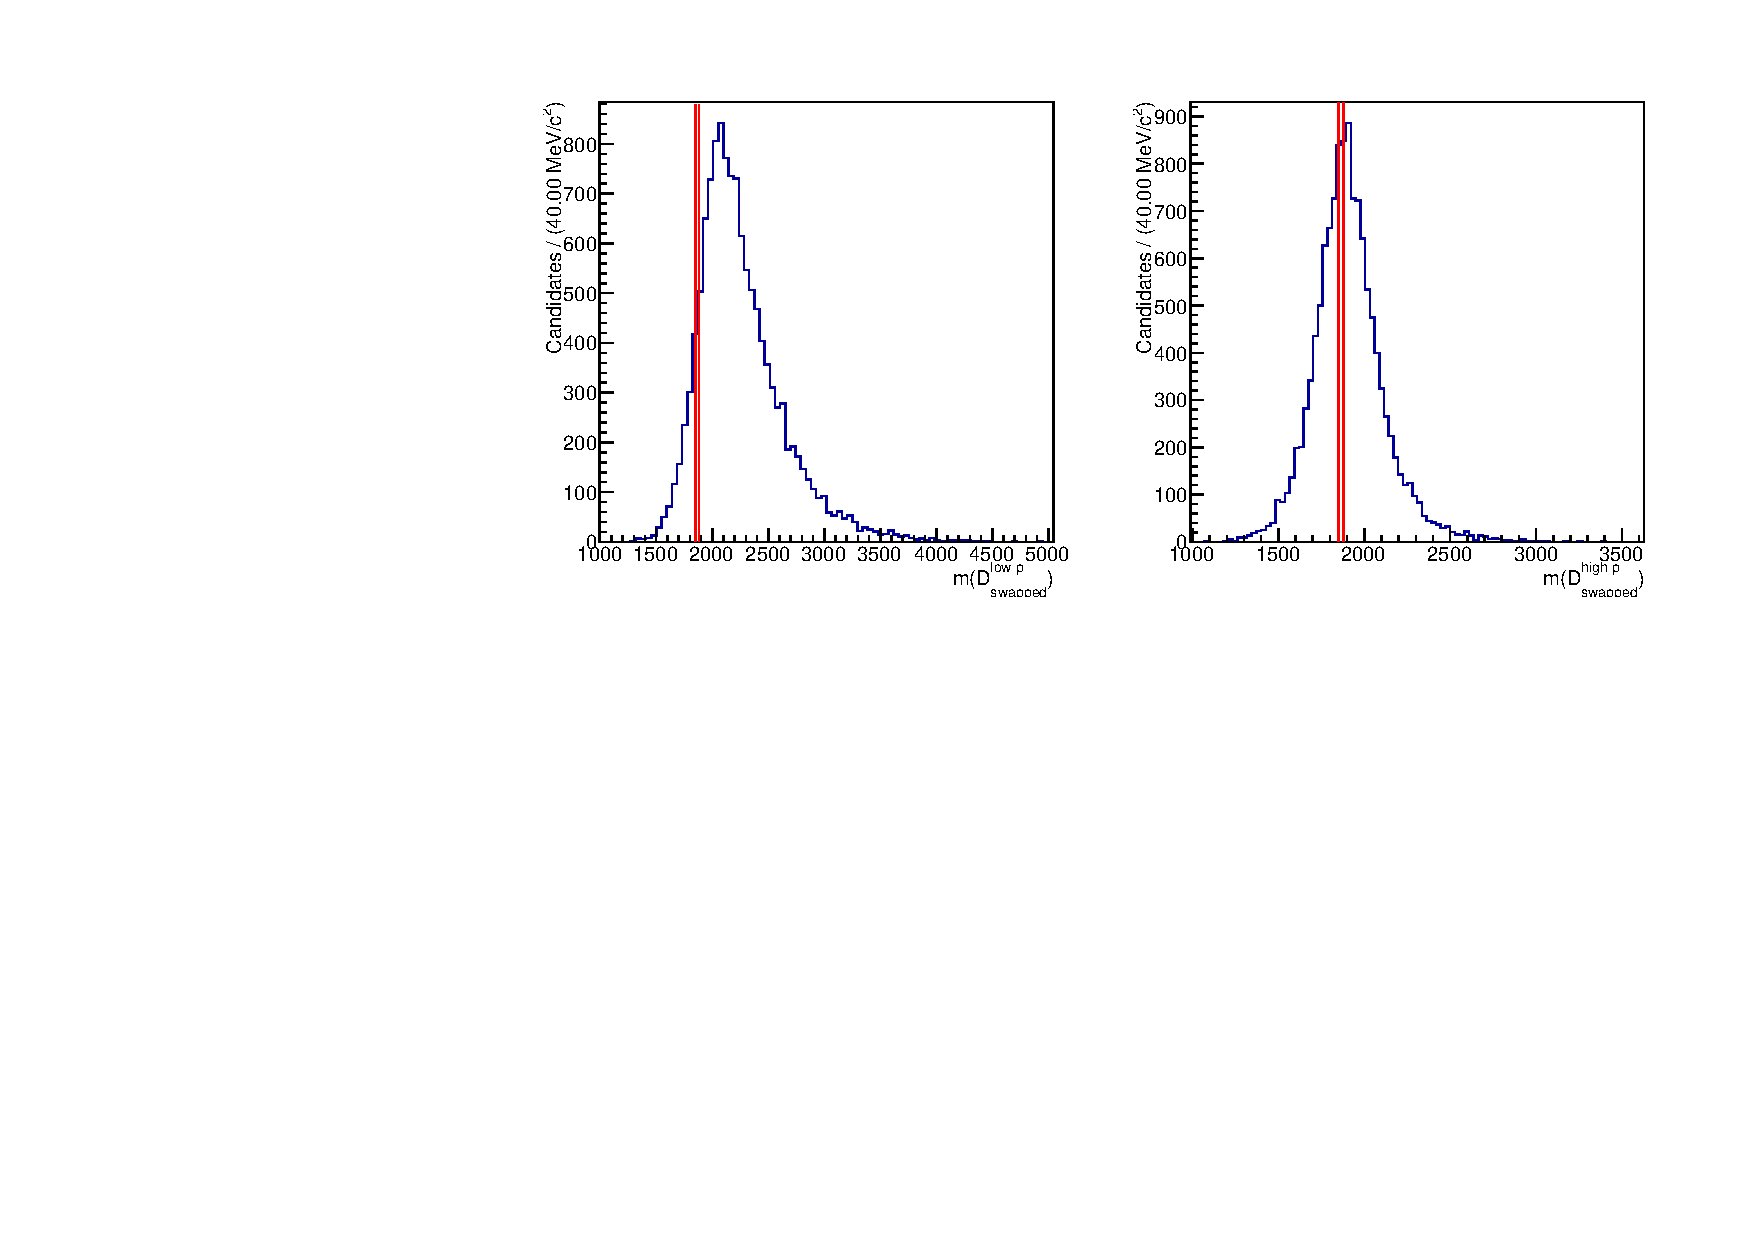
\includegraphics[width=\linewidth]{figures/backgrounds/Dmassveto_4body.pdf}
\put(-380,150) {(a)}
\put(-170,150) {(b)}
\caption{Distributions from simulated samples for DD canidates in Run 2 showing the swapped \Dz daughter mass hypothesis where (a) the kaon is swapped with the lower momentum pion and (b) the kaon is swapped with the higher momentum pion. The red lines correspond to the double misID veto selection window applied to the suppressed mode.}
\label{Dmassveto4body}
\end{figure}

In order to determine the overall crossfeed contamination in the supressed \pik mode the efficiency of the \Dz mass window, double misidentification veto and PID requirements are taken into account for both the normal and swapped \Dz mass hypothesis. 
%For the two-body mode, these efficiencies are listed in Tables \ref{crossfeedefficienciesRun1} and \ref{crossfeedefficienciesRun2}. 
The proportion of events expected in the \Bm mass spectrum of the supressed \pik mode relative to the total \pik is estimated to be $9.5 \times 10^{-3}$ for LL and $6.5 \times 10^{-3}$ for DD in Run 1, and $5.6 \times 10^{-3}$ for LL and $5.3 \times 10^{-3}$ in Run 2. Similarly for the 4-body mode, proportion of events expected in the \Bm mass spectrum of the supressed \pikpipi mode relative to the total \pikpipi is estimated to be $2.7 \times 10^{-3}$ for LL and $1.0 \times 10^{-3}$ for DD in Run 1, and $1.4 \times 10^{-3}$ for LL and $6.3 \times 10^{-4}$ in Run 2. Therefore, the contribtuion of the crossfeed in both the two- and four-body ADS modes is negligible at less than 0.1\% of the signal.

%The tighter BDT cut applied in the ADS mode for DD candidates also has to be taken into account. The relative BDT efficiency is 0.877 for Run 1 and 0.902 for Run 2.
%{\footnotesize
%\begin{table}[h]
%\centering
%\begin{tabular}{ccc}
%\hline
%Selection cut & $[K_K^-\pi_\pi^+]_D$ efficiency & $[K_\pi^-\pi_K^+]_D$ efficiency \\
%\hline
%\Dz window: $\pm$ 25 MeV & 0.961 $\pm$ 0.003 & 0.116 $\pm$ 0.005 \\
%Crossfeed veto $\pm$ 15 MeV & 0.930 $\pm$ 0.004 & 0.122 $\pm$ 0.014 \\
%PID selection & 0.734 $\pm$ 0.002 & 0.00158 $\pm$ 0.00002 \\
%\hline
%Total & 0.655 $\pm$ 0.004 & (2.2 $\pm$ 0.3) $\times 10^{-5}$ \\
%\hline
%\end{tabular}
%\begin{tabular}{ccc}
%\hline
%Selection cut & $[K_K^-\pi_\pi^+]_D$ efficiency & $[K_\pi^-\pi_K^+]_D$ efficiency \\
%\hline
%\Dz window: $\pm$ 25 MeV & 0.961 $\pm$ 0.002 & 0.123 $\pm$ 0.003 \\
%Crossfeed veto $\pm$ 15 MeV & 0.925 $\pm$ 0.002 & 0.087 $\pm$ 0.007 \\
%PID selection & 0.747 $\pm$ 0.002 & 0.00144 $\pm$ 0.00005 \\
%\hline
%Total & 0.663 $\pm$ 0.003 & (1.53 $\pm$ 0.14) $\times 10^{-5}$ \\
%\hline
%\end{tabular}
%\caption{Efficiencies of the \Dz mass window, crossfeed veto and \Dz daughter PID cuts for \decay{\Bpm}{[\Kmp\pipm]_D\Kstarpm} events in Run 1. The first table shows the LL efficiencies and the second shows the DD efficiencies. The proprtion of crossfeed events from favoured \decay{\Bpm}{[\Kpm\pimp]_D\Kstarpm} mode which are expected in \decay{\Bpm}{[\Kmp\pipm]_D\Kstarpm} mode fit is $(9.5 \pm 1.2) \times 10^{-3}$ for LL and $(6.5 \pm 0.6) \times 10^{-3}$ for DD}
%\label{crossfeedefficienciesRun1}
%\end{table}
%
%\begin{table}
%\centering
%\begin{tabular}{ccc}
%\hline
%Selection cut & $[K_K^-\pi_\pi^+]_D$ efficiency & $[K_\pi^-\pi_K^+]_D$ efficiency \\
%\hline
%\Dz window: $\pm$ 25 MeV & 0.954 $\pm$ 0.002 & 0.118 $\pm$ 0.003 \\
%Crossfeed veto $\pm$ 15 MeV & 0.929 $\pm$ 0.003 & 0.108 $\pm$ 0.009 \\
%PID selection & 0.811 $\pm$ 0.002 & 0.00112 $\pm$ 0.00002 \\
%\hline
%Total & 0.719 $\pm$ 0.003 & (1.43 $\pm$ 0.12) $\times 10^{-5}$ \\
%\hline
%\end{tabular}
%\begin{tabular}{ccc}
%\hline
%Selection cut & $[K_K^-\pi_\pi^+]_D$ efficiency & $[K_\pi^-\pi_K^+]_D$ efficiency \\
%\hline
%\Dz window: $\pm$ 25 MeV & 0.9553 $\pm$ 0.0012 & 0.1181 $\pm$ 0.0019 \\
%Crossfeed veto $\pm$ 15 MeV & 0.9284 $\pm$ 0.0016 & 0.111 $\pm$ 0.005 \\
%PID selection & 0.821 $\pm$ 0.002 & 0.00104 $\pm$ 0.00002 \\
%\hline
%Total & 0.728 $\pm$ 0.002 & (1.37 $\pm$ 0.08) $\times 10^{-5}$ \\
%\hline
%\end{tabular}
%\caption{Efficiencies of the \Dz mass window, crossfeed veto and \Dz daughter PID cuts for \decay{\Bpm}{[\Kmp\pipm]_D\Kstarpm} events in Run 2. The first table shows the LL efficiencies and the second shows the DD efficiencies. The proprtion of crossfeed events from favoured \decay{\Bpm}{[\Kpm\pimp]_D\Kstarpm} mode which are expected in \decay{\Bpm}{[\Kmp\pipm]_D\Kstarpm} mode fit is $(5.6 \pm 0.5) \times 10^{-3}$ for LL and $(5.3 \pm 0.3) \times 10^{-3}$ for DD}
%\label{crossfeedefficienciesRun2}
%\end{table}}
%
%\begin{table}[h]
%\centering
%\begin{tabular}{ccc}
%\hline
%Selection cut & $[K_K^-\pi_\pi^+\pim\pip]_D$ efficiency & $[K_\pi^-\pi_K^+\pim\pip]_D$ efficiency \\
%\hline
%\Dz window: $\pm$ 25 MeV & 0.749 $\pm$ 0.011 & 0.009 $\pm$ 0.002 \\
%Crossfeed veto $\pm$ 15 MeV & 0.907 $\pm$ 0.008 & 0.50 $\pm$ 0.13 \\
%PID selection & 0.630 $\pm$ 0.002 & 0.00089 $\pm$ 0.00002 \\
%\hline
%Total & 0.428 $\pm$ 0.007 & (3.8 $\pm$ 1.4) $\times 10^{-6}$ \\
%\hline
%\end{tabular}
%\begin{tabular}{ccc}
%\hline
%Selection cut & $[K_K^-\pi_\pi^+\pim\pip]_D$ efficiency & $[K_\pi^-\pi_K^+\pim\pip]_D$ efficiency \\
%\hline
%\Dz window: $\pm$ 25 MeV & 0.817 $\pm$ 0.006 & 0.0080 $\pm$ 0.0013 \\
%Crossfeed veto $\pm$ 15 MeV & 0.904 $\pm$ 0.005 & 0.23 $\pm$ 0.07 \\
%PID selection & 0.636 $\pm$ 0.002 & 0.00084 $\pm$ 0.00002 \\
%\hline
%Total & 0.470 $\pm$ 0.004 & (1.54 $\pm$ 0.5) $\times 10^{-6}$ \\
%\hline
%\end{tabular}
%\caption{Efficiencies of the \Dz mass window, crossfeed veto and \Dz daughter PID cuts for \decay{\Bpm}{[\Kmp\pipm\pimp\pipm]_D\Kstarpm} events in Run 1. The first table shows the LL efficiencies and the second shows the DD efficiencies. The proprtion of crossfeed events from favoured \decay{\Bpm}{[\Kpm\pimp\pipm\pimp]_D\Kstarpm} mode which are expected in \decay{\Bpm}{[\Kmp\pipm\pimp\pipm]_D\Kstarpm} mode fit is $(2.7 \pm 1.0) \times 10^{-3}$ for LL and $(1.0 \pm 0.4) \times 10^{-3}$ for DD}
%\label{crossfeedefficienciesk3piRun1}
%\end{table}
%
%\begin{table}
%\centering
%\begin{tabular}{ccc}
%\hline
%Selection cut & $[K_K^-\pi_\pi^+\pim\pip]_D$ efficiency & $[K_\pi^-\pi_K^+\pim\pip]_D$ efficiency \\
%\hline
%\Dz window: $\pm$ 25 MeV & 0.791 $\pm$ 0.003 & 0.0072 $\pm$ 0.0007 \\
%Crossfeed veto $\pm$ 15 MeV & 0.905 $\pm$ 0.003 & 0.31 $\pm$ 0.05 \\
%PID selection & 0.784 $\pm$ 0.002 & 0.00115 $\pm$ 0.00002 \\
%\hline
%Total & 0.561 $\pm$ 0.003 & (2.6 $\pm$ 0.5) $\times 10^{-6}$ \\
%\hline
%\end{tabular}
%\begin{tabular}{ccc}
%\hline
%Selection cut & $[K_K^-\pi_\pi^+\pim\pip]_D$ efficiency & $[K_\pi^-\pi_K^+\pim\pip]_D$ efficiency \\
%\hline
%\Dz window: $\pm$ 25 MeV & 0.820 $\pm$ 0.002 & 0.0057 $\pm$ 0.0004 \\
%Crossfeed veto $\pm$ 15 MeV & 0.9040 $\pm$ 0.0018 & 0.20 $\pm$ 0.03\\
%PID selection & 0.798 $\pm$ 0.002 & 0.00106 $\pm$ 0.00002 \\
%\hline
%Total & 0.592 $\pm$ 0.002 & (1.2 $\pm$ 0.2) $\times 10^{-6}$ \\
%\hline
%\end{tabular}
%\caption{Efficiencies of the \Dz mass window, crossfeed veto and \Dz daughter PID cuts for \decay{\Bpm}{[\Kmp\pipm\pimp\pipm]_D\Kstarpm} events in Run 2. The first table shows the LL efficiencies and the second shows the DD efficiencies. The proprtion of crossfeed events from favoured \decay{\Bpm}{[\Kpm\pimp\pipm\pimp]_D\Kstarpm} mode which are expected in \decay{\Bpm}{[\Kmp\pipm\pimp\pipm]_D\Kstarpm} mode fit is $(1.4 \pm 0.3) \times 10^{-3}$ for LL and $(6.3 \pm 1.1) \times 10^{-4}$ for DD}
%\label{crossfeedefficienciesk3piRun2}
%\end{table}}

\subsubsection{\boldmath \decay{\Lb}{\Lc\Kstar} background for \decay{\D}{\Kp\Km} fit}
\label{sec:backgrounds:Lb2LcKst}

An additional source of background in the \kk \Bm mass spectrum comes from the decay \decay{\Lb}{\Lc(p\kaon\pi)\Kstarm}, where the proton is misidentified as a kaon and the \pion is missed in the reconstruction. The \decay{\Bm}{\D\Km} analysis~\cite{LHCb-PAPER-2016-003} also included an equivalent \decay{\Lb}{\Lc(p\kaon\pi)\Km} background. The shape used to model this contribution is a RooCruijff PDF, defined as,
\begin{equation}
  \mathrm{Cruijff}(m; \mu,\sigma_L,\sigma_R,\alpha_L,\alpha_R)=
\begin{cases}
    exp \left( -\frac{(m-\mu)^2}{2\sigma_L^2 + \alpha_L(m-\mu)^2} \right) ,     & \text{if } m-\mu < 0, \\
    exp \left( -\frac{(m-\mu)^2}{2\sigma_R^2 + \alpha_R(m-\mu)^2} \right) ,     & \text{otherwise.}
\end{cases}
\label{Cruijff}
\end{equation}%
where $\mu$ is the peak, $\sigma_{L,R}$ is the width on the left and right sides of the peak and $\alpha_{L,R}$ is a modification constant. These shape parameters taken from a fit to a simulated sample of \decay{\Lb}{\Lc\Km} events reconstructed as \decay{\Bm}{\D\Km} events, as a simulated samples of \decay{\Lb}{\Lc\Kstarm} events is not available and the shapes are expected to be similar.

The fit to the \Bm mass spectrum is shown in Figure \ref{Lbfit}, where it can be seen that the reconstructed \Bm mass falls between 4800 and 5500 \mevcc, and the results from this fit are shown in Table \ref{fitresultsLb}. All the values for the shape parameters are fixed in the simultaneous fit to the values in Table \ref{fitresultsLb}, which is considered to be a source of systematic uncertainty, detailed in Section \ref{sec:systematics}. 

\begin{figure}[h]
\centering
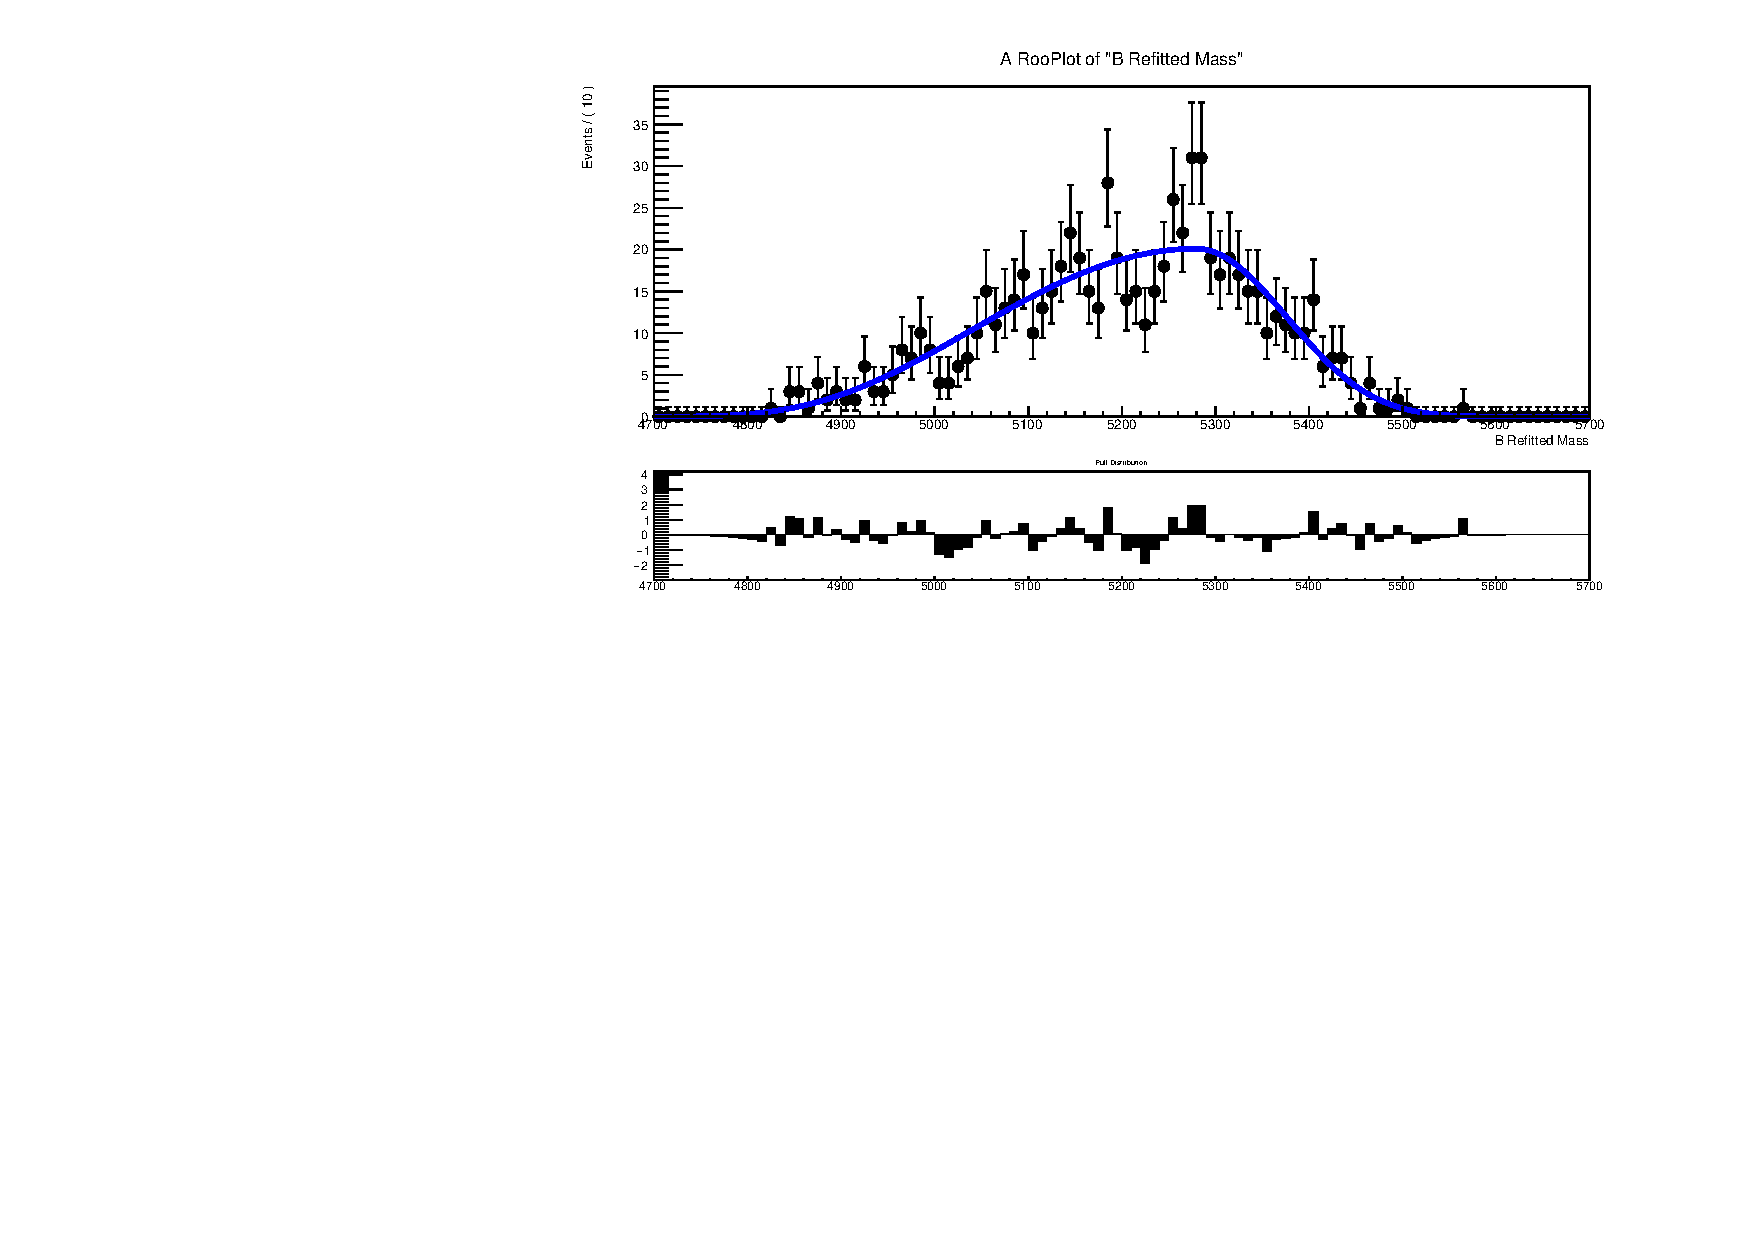
\includegraphics[width=0.7\linewidth]{figures/backgrounds/Lb2LcKst.pdf}
\caption{Fit to \decay{\Lb}{\Lc(pK\pi)\kaon} MC using a RooCruijff PDF, where the \pion is missed in reconstruction and the proton is misidentified as a kaon. This contributes as a source of background in the \decay{\Bm}{\D\Kstarm}, \decay{\D}{\Kp\Km} fit.}
\label{Lbfit}
\end{figure}

\begin{table}[h]
\centering
\begin{tabular}{cc}
\hline
Parameter & Value \\
\hline
$\mu$ & $5280 \pm 18$ \\
$\sigma_L$ & $221 \pm 26$ \\
$\sigma_R$ & $96 \pm 16$ \\
$\alpha_L$ & $-0.19 \pm 0.19$ \\
$\alpha_R$ & $-0.04 \pm 0.06$ \\
\hline
\end{tabular}
\caption{Shape parameters from a fit to simulated \decay{\Lb}{\Lc\Km} events using a RooCruijff PDF. These shape parameters are fixed with an associated systematic uncertainty.}
\label{fitresultsLb}
\end{table}

The shape is assumed to be the same in each \kk fit category. The \decay{\Lb}{\Lc(p\kaon\pi)\Kstarm} yield compared to the signal yield in the favoured \kpi mode is allowed to vary in the simultaneous fit. This fractional yield is required to be the same for all fit categories. 

%\subsubsection{\boldmath Other \Lb backgrounds}
%\label{sec:backgrounds:lambda}
%
%Other possible backgrounds from \Lb decays are discussed in this section. In each of the cases a pion is missed in reconstruction and the proton is misidentified as a kaon. Also, the bachelor has the opposite sign as the proton (misidentified as a kaon), therefore it is a background for the ADS mode and so would not be related to the combinatoric discrepancy discussed in Section \ref{sec:app:combinatoric}. The backgrounds considered for investigation are:
%
%\begin{itemize}
%\item {\decay{\Lb}{\Lc(p\KS\pi\pi)\pi}: The selection efficiency for \decay{\Lb}{\Lc\pi} through the $K\pi$ selection would be much lower than \decay{\Lb}{\Lc\Kstar} through the $KK$ selection, as:
%	\begin{itemize}
%		\item \decay{\Lb}{\Lc\Kstar} would pass the \Kstar selection requirements that \decay{\Lb}{\Lc\pi} would not
%		\item In \decay{\Lb}{\Lc\pi} the \KS would not point towards the \B vertex as required.
%	\end{itemize}  
%Although the backgrounds are contributing to a different mode a comparison in selection efficiency can still be drawn. These decays have similar branching fractions. Therefore, the \decay{\Lb}{\Lc\pi} background in $K\pi$ would contribute much less than the \decay{\Lb}{\Lc\Kstar} background in $KK$ (much less than 0.5\%), and is therefore ignored}
%\item \decay{\Lb}{\Lc(p\pi\pi)\Kstar}: The \decay{\Lc}{p\pi\pi} background for $K\pi$ would be too small to contribute as the branching fraction is over a factor of 10 smaller than \decay{\Lc}{p\pi\pi} (0.4\% compared to 6.3\%~\cite{PDG2016}) and the contribution of \decay{\Lc}{pK\pi} in the $KK$ mode was less than 0.5\%.
%\item \decay{\Lb}{\Lc(\Lambda(p\pi)\pi)\Kstar}
%\item \decay{\Lb}{\Lc(\Lambda(p\pi)\pi\piz)\Kstar}
%\item \decay{\Lb}{\Lc(\Lambda(p\pi)\pi\pi\pi)\Kstar} for \decay{\Bm}{\D(\Kp\pim\pip\pim)\Kstarm}
%\end{itemize}
%
%The last three possibilities that decay via a $\Lambda$ would not pass the selection due to the topological constraints. The reconstructed \D would not point back to the \D decay vertex due to the missed pion, resulting in a poor \B vertex. Therefore, all the \Lb backgrounds discussed in this section are considered negligible in this analysis.

\subsubsection{\boldmath \decay{\Bs}{\Dzb\bar{K}^{*}(1410)^0} background}
\label{sec:backgrounds:bs}

The decay \decay{\Bs}{\Dzb\bar{K}^{*}(1410)^0} or $\Dzb K_1(1400)^0$, \decay{(K_1,K^*)}{K^{*}(892)^-\pip}, where the \pip is missed in reconstruction could contribute region of the \pik ADS mode just below the \Bm mass peak. In the \decay{\Bm}{\D h^-} analysis~\cite{LHCb-PAPER-2016-003} the equivalent \decay{\Bs}{\D K^*(892)^0} background is a significant contribution to the model in the \pik ADS mode and contributes to the \Bm mass spectrum in the region containing the signal peak. In this analysis the low mass limit of the simultaneous fit is at 5230 \mev and therefore this background will be almost entirely removed. However, it is possible that a small contribution still remains and contributes to the signal region. Figure \ref{adsfullrange} shows the \B mass distribution over the full mass range for the \kpi and \pik modes. The \pik mode does not have many events and therefore it is difficult to draw any conclusions from this plot, however, the signal and partially reconstructed background can be seen. There is also possible evidence of an excess at about 5180\mev.

\begin{figure}
\centering
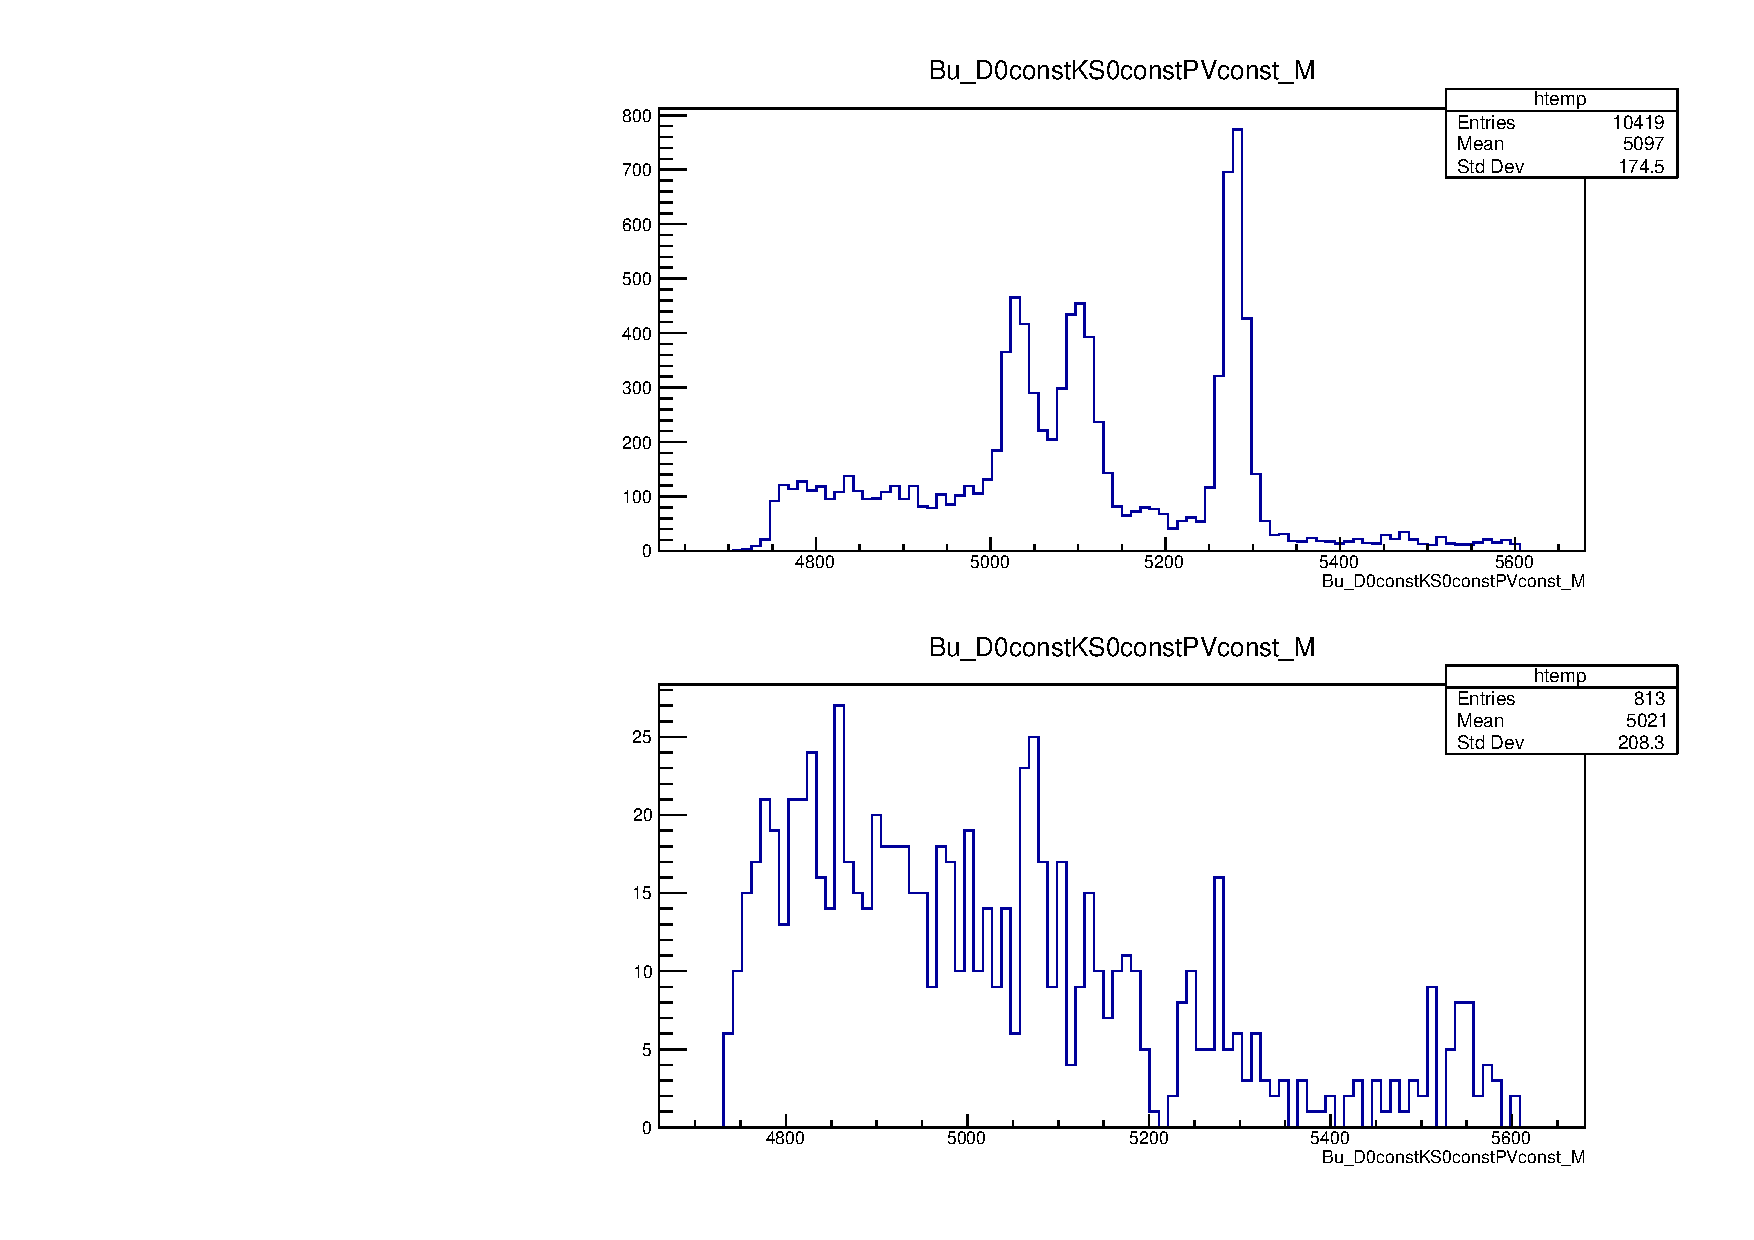
\includegraphics[width=0.6\linewidth]{figures/backgrounds/adsfullrange.pdf}
\caption{\B mass distribution for both the charge favoured \kpi mode (top) and the ADS mode (bottom) after the full selection, summed over run period and \KS reconstruction type.}
\label{adsfullrange}
\end{figure}

In order to obtain an idea of how much this \Bs background would contribute to the \Bm mass spectrum, and as such affect the results of the fit, a simple fit to data was performed to the \pik mode from 5150 - 5600 \mev in \Bm mass. The shape of the \Bs background generated using RapidSim, as shown in Figure \ref{Bsshape}, is subsequently fitted using a one-dimensional kernal estimation probability density function. The model used to perform a fit to the \Bm mass spectrum in the \pik mode consists of a Gaussian signal shape, combinatorial described by an exponential and the \Bs background shape described. As there are so few events in the ADS mode the signal shape parameters were fixed from the full fit in order to maintain fit stability. The fit described is shown in Figure \ref{adsfit}. It can be seen that $\sim$2 \Bs events enter the simultaneous fit region above 5230\mev.

\begin{figure}
\centering
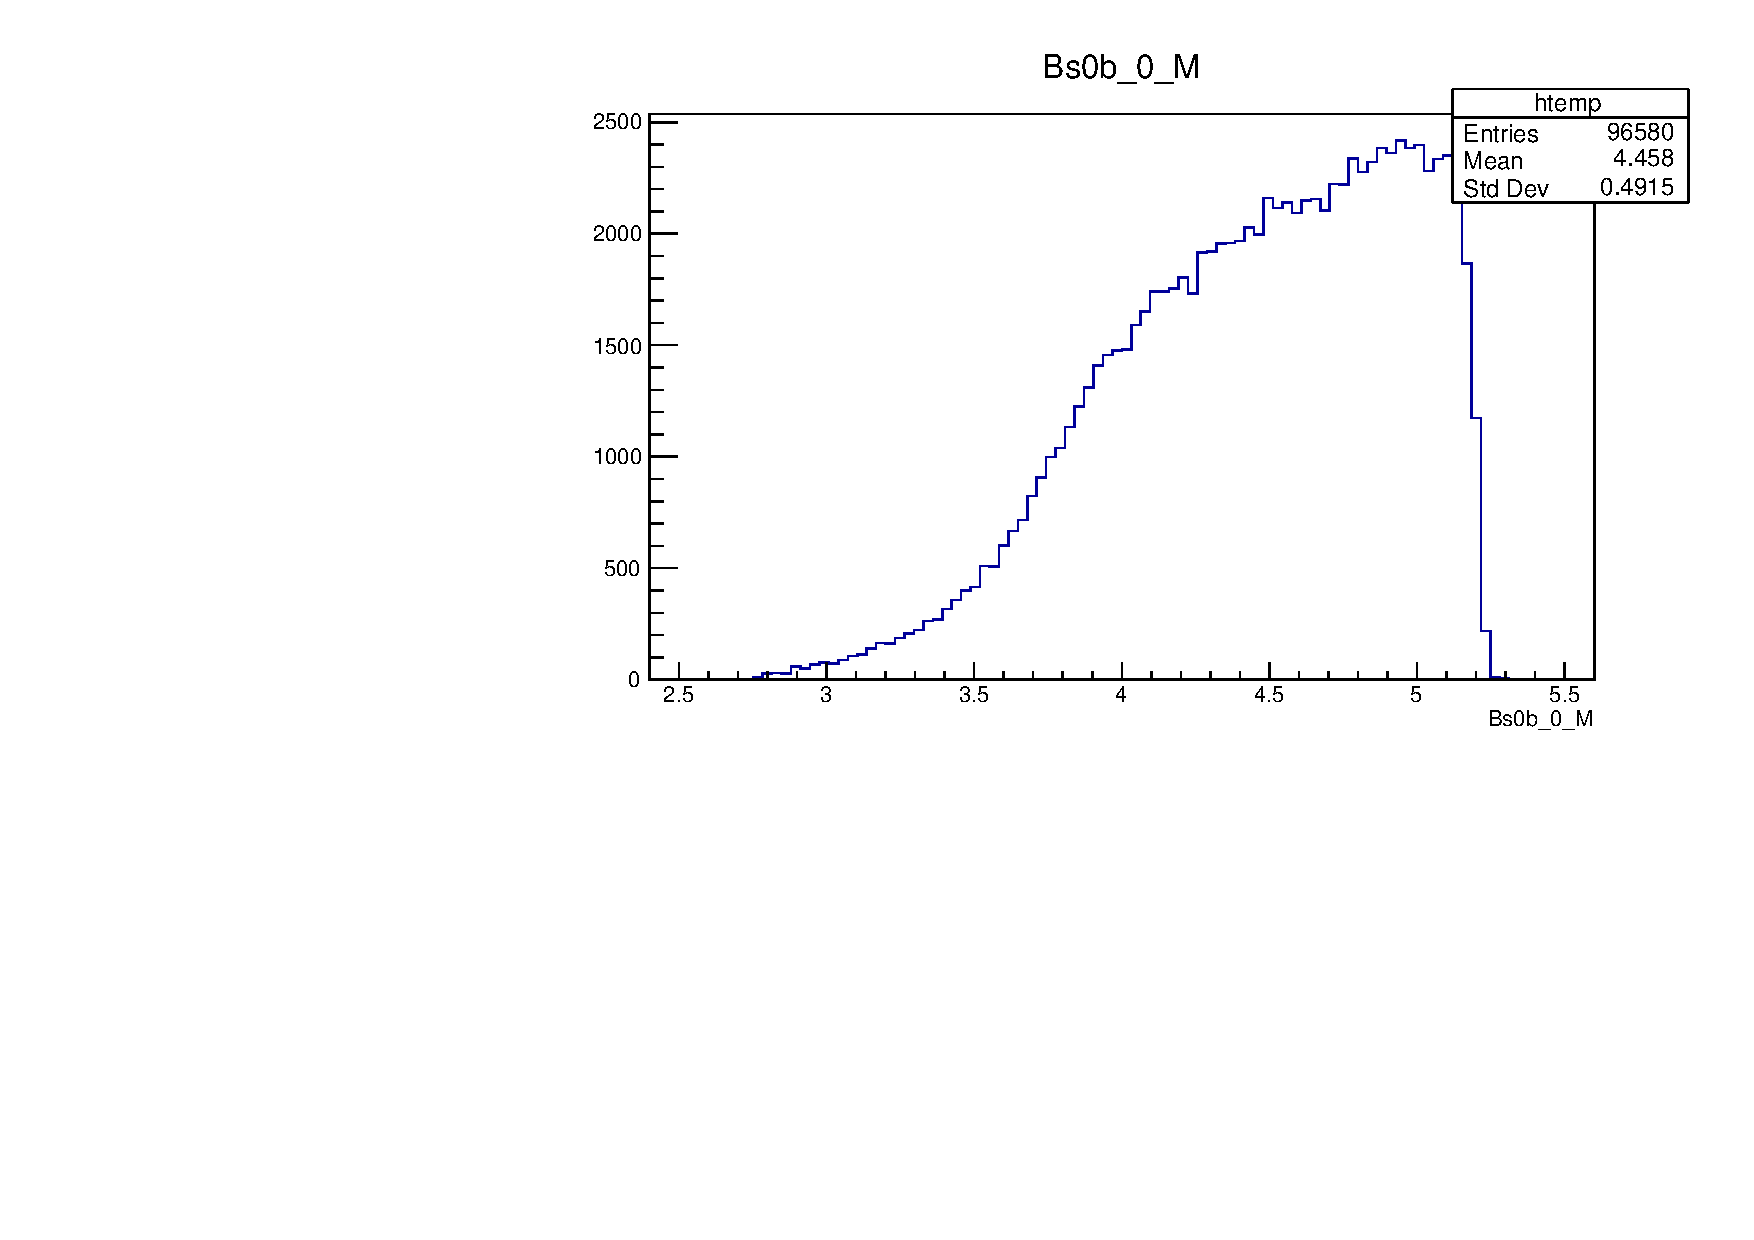
\includegraphics[width=0.5\linewidth]{figures/backgrounds/BsShape.pdf}
\caption{Simulation of \decay{\Bs}{\Dzb\bar{K}^{*}(1410)^0}, \decay{\bar{K}^{*}(1410)^0}{K^{*}(892)^-\pip}, where the \pip is missed in reconstruction, generated using RapidSim. The \decay{\Bs}{\Dzb\bar{K}_1(1400)^0} has a very similar shape.}
\label{Bsshape}
\end{figure}

\begin{figure}
\centering
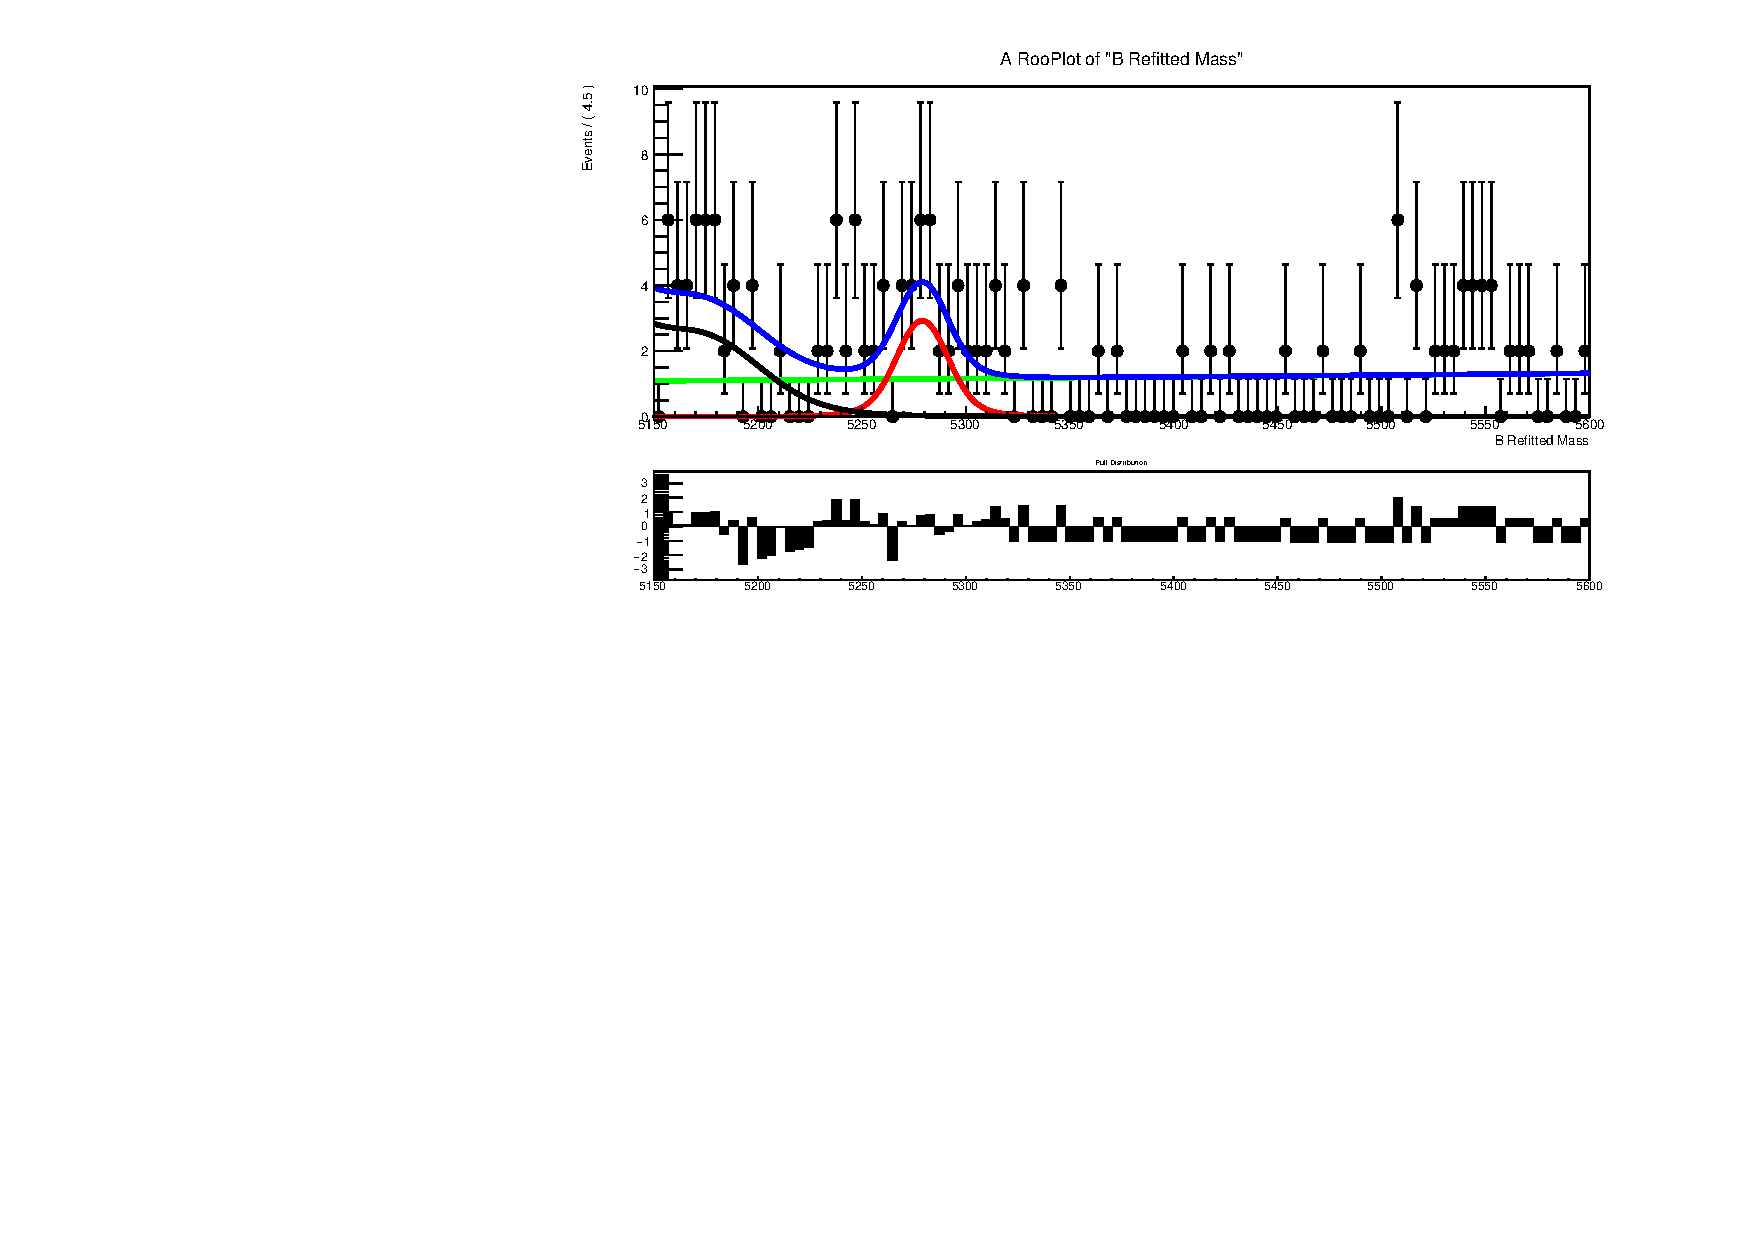
\includegraphics[width=0.7\linewidth]{figures/backgrounds/adsfit.pdf}
\caption{Simple fit to data of the \B mass distribution in the ADS mode from 5150\mev. The components are the signal (red), combinatorial (green) and \Bs background (black).}
\label{adsfit}
\end{figure}

Alternatively, the \Bs background contribution can be estimated by using the \decay{\Bs}{\Dzb\bar{K}^{*}(1410)^0} branching fraction of $\left(3.9 \pm 3.5\right) \times 10^{-4}$~\cite{PDG2016} and the efficiency \Bm mass requirement being greater than 5230\mev taken from the \Bs shape in Figure \ref{Bsshape}, which is $6.4 \times 10^{-4}$. This gives an estimate of $2.6 \pm 2.6$ \decay{\Bs}{\Dzb\bar{K}^{*}(1410)^0} events in \pik mode above 5230\mev, which is consistent with the estimate from Figure \ref{adsfit}. This estimated \Bs background is used to assign a systematic uncertainty to the \CP observables, discussed in more detail in Section \ref{sec:systematics}.


\subsubsection{Lambda contamination}
\label{sec:backgrounds:contamination}

The \decay{\KS}{\pip\pim} decay could have contamination coming from \decay{\Lz}{\proton\pim}, where the proton is reconstructed as a pion. It is not possible to determine possible \Lz contamination from the \KS invariant mass spectrum, where one of the \KS daughters is assigned the proton mass, because a peak at the \Lz mass cannot be distinguished from the variation near the low mass threshold. In order to distinguish between \KS decays and \Lz contamination the Armenteros-Podolanski (AP) plot is used~\cite{APplot}. The transverse momentum of the daughters with respect to the mother particle, $p_T$, is plotted against the longitudinal momentum asymmetry, which is defined as,

\begin{equation}
\frac{p_L^+ - p_L^-}{p_L^+ + p_L^-}
\label{longitudinalpasy}
\end{equation}

where $p_L^{\pm}$ is the longitudinal momentum of the daughter particles with respect to the direction of the mother. The resulting AP plots for both data and simulation are shown in Figure \ref{applots}. The decay products of the \decay{\KS}{\pip\pim} decay have the same mass and therefore on average their momenta is symmetrically distributed, resulting in the distribution observed in Figure \ref{applots}; these curves are the same shape as the expected distribution for a sample of pure \KS mesons. Whereas for the \decay{\Lz}{\proton\pim}, the proton would, on average, take a larger proportion of the momentum resulting in an asymmteric distribution. Contamination from \Lz baryons would be clearly seen as a distinct structure on the AP plot, as illustrated in Figure \ref{apexample}. Therefore, Figure \ref{applots} shows that there is no contamination from \decay{\Lz}{\proton\pim} decays in the data.
%The distribution of the events in the data sample can be seen more clearly in Figure \ref{applotsdata}.

\begin{figure}[h]
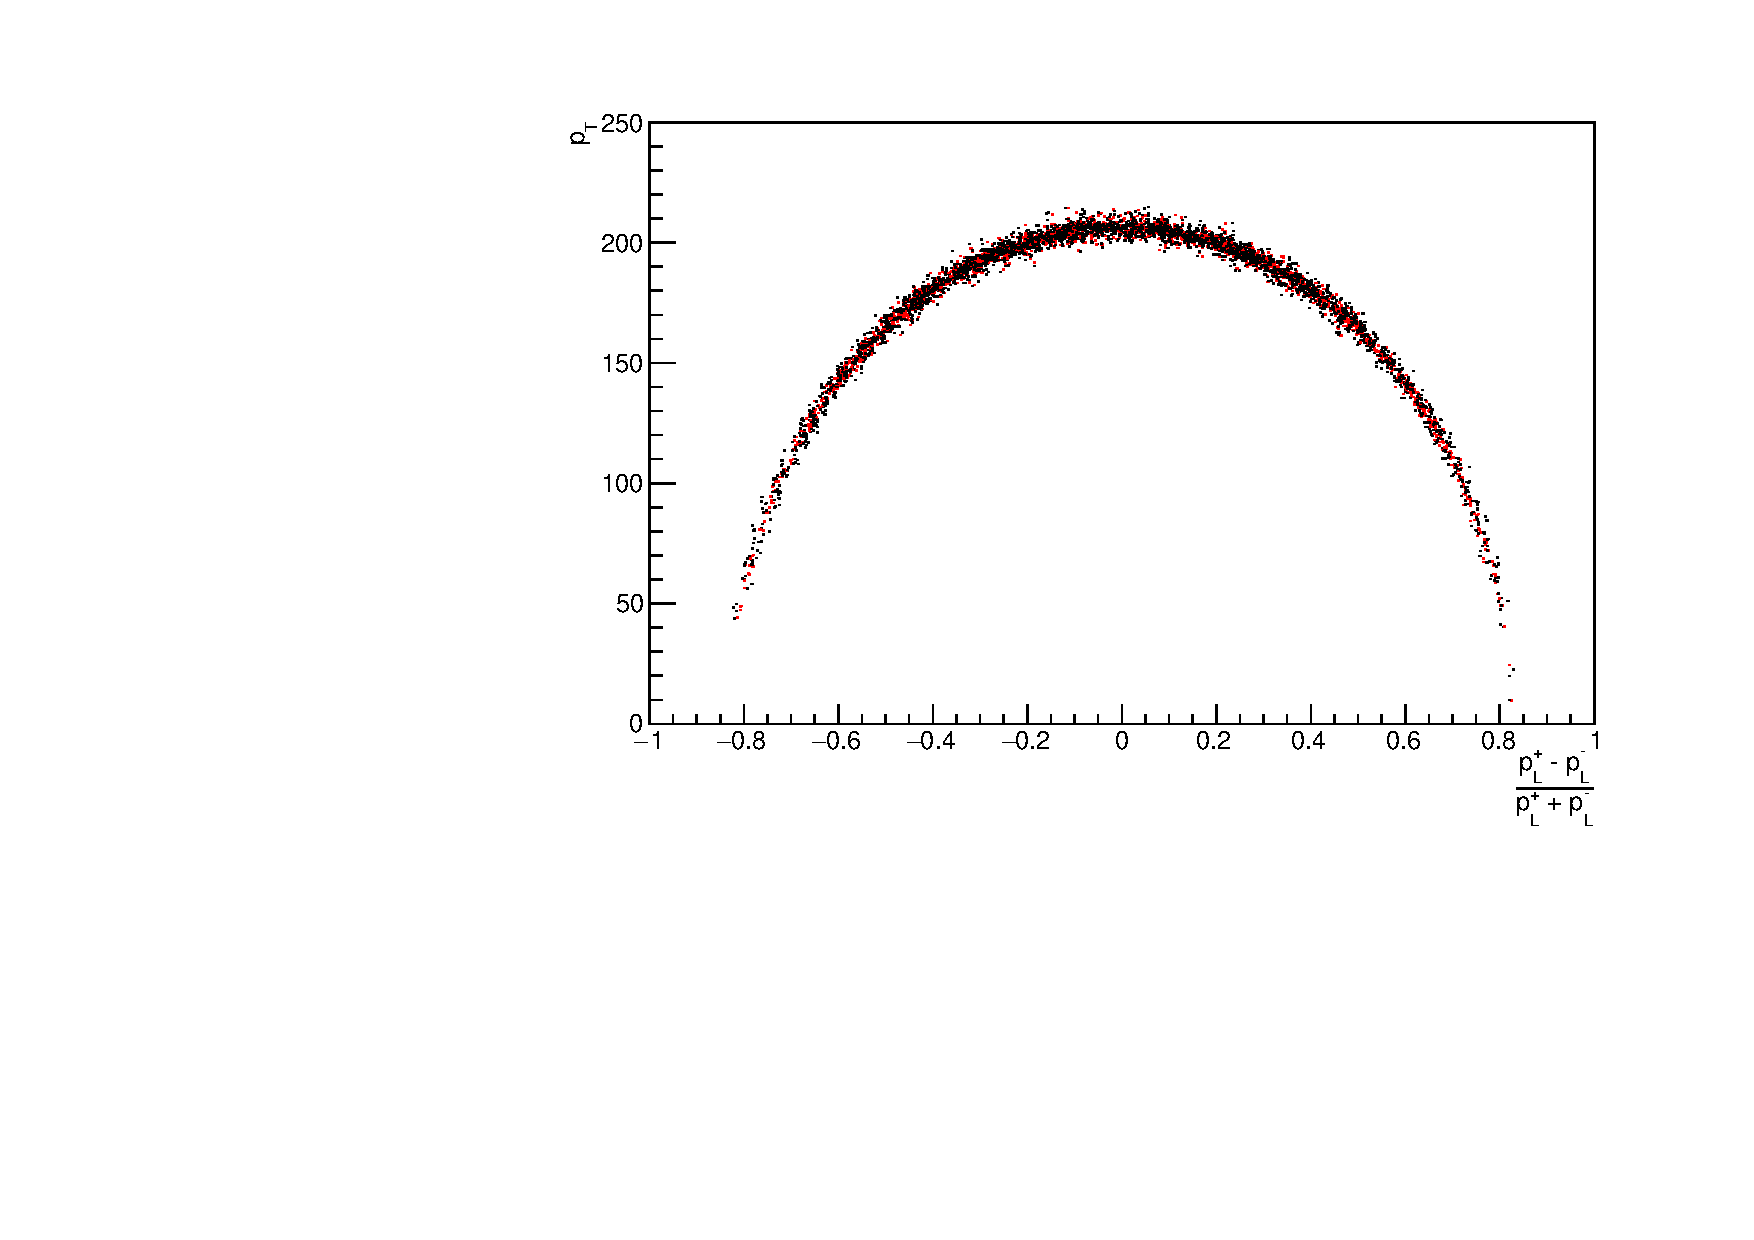
\includegraphics[width=0.5\linewidth]{figures/backgrounds/APplot_LL.pdf}
\put(-180,100) {(a)}
\hfill
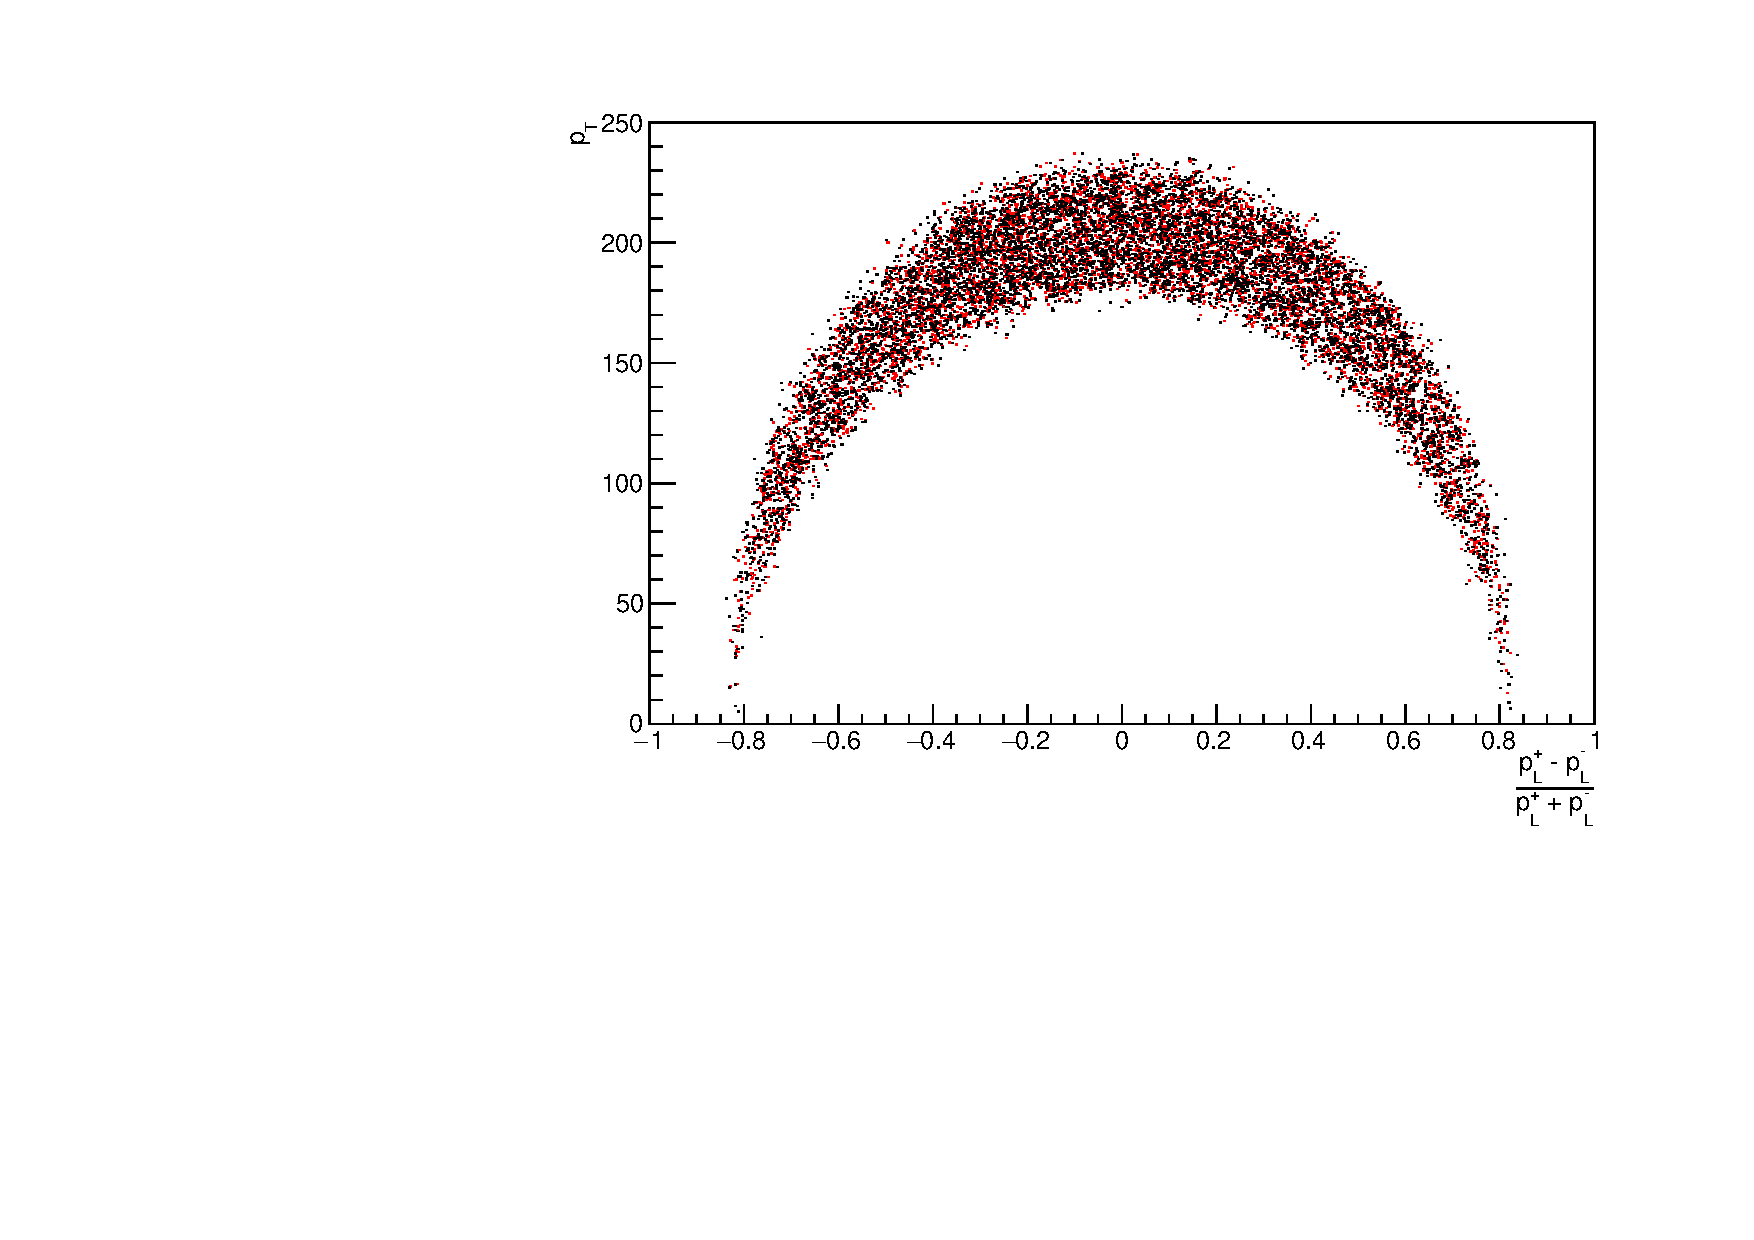
\includegraphics[width=0.5\linewidth]{figures/backgrounds/APplot_DD.pdf}
\put(-180,100) {(b)}
\caption{Armenteros-Podolanski plots for both data (black) and simulation (red) for (a) LL, and (b) DD canididates. The $p_T$ values on the y axis are the transverse momentum of the daughters with respect to the mother particle and the x axis contains the longitudinal momentum asymmetry, defined in Equation \ref{longitudinalpasy}.}
\label{applots}
\end{figure}

%\begin{figure}
%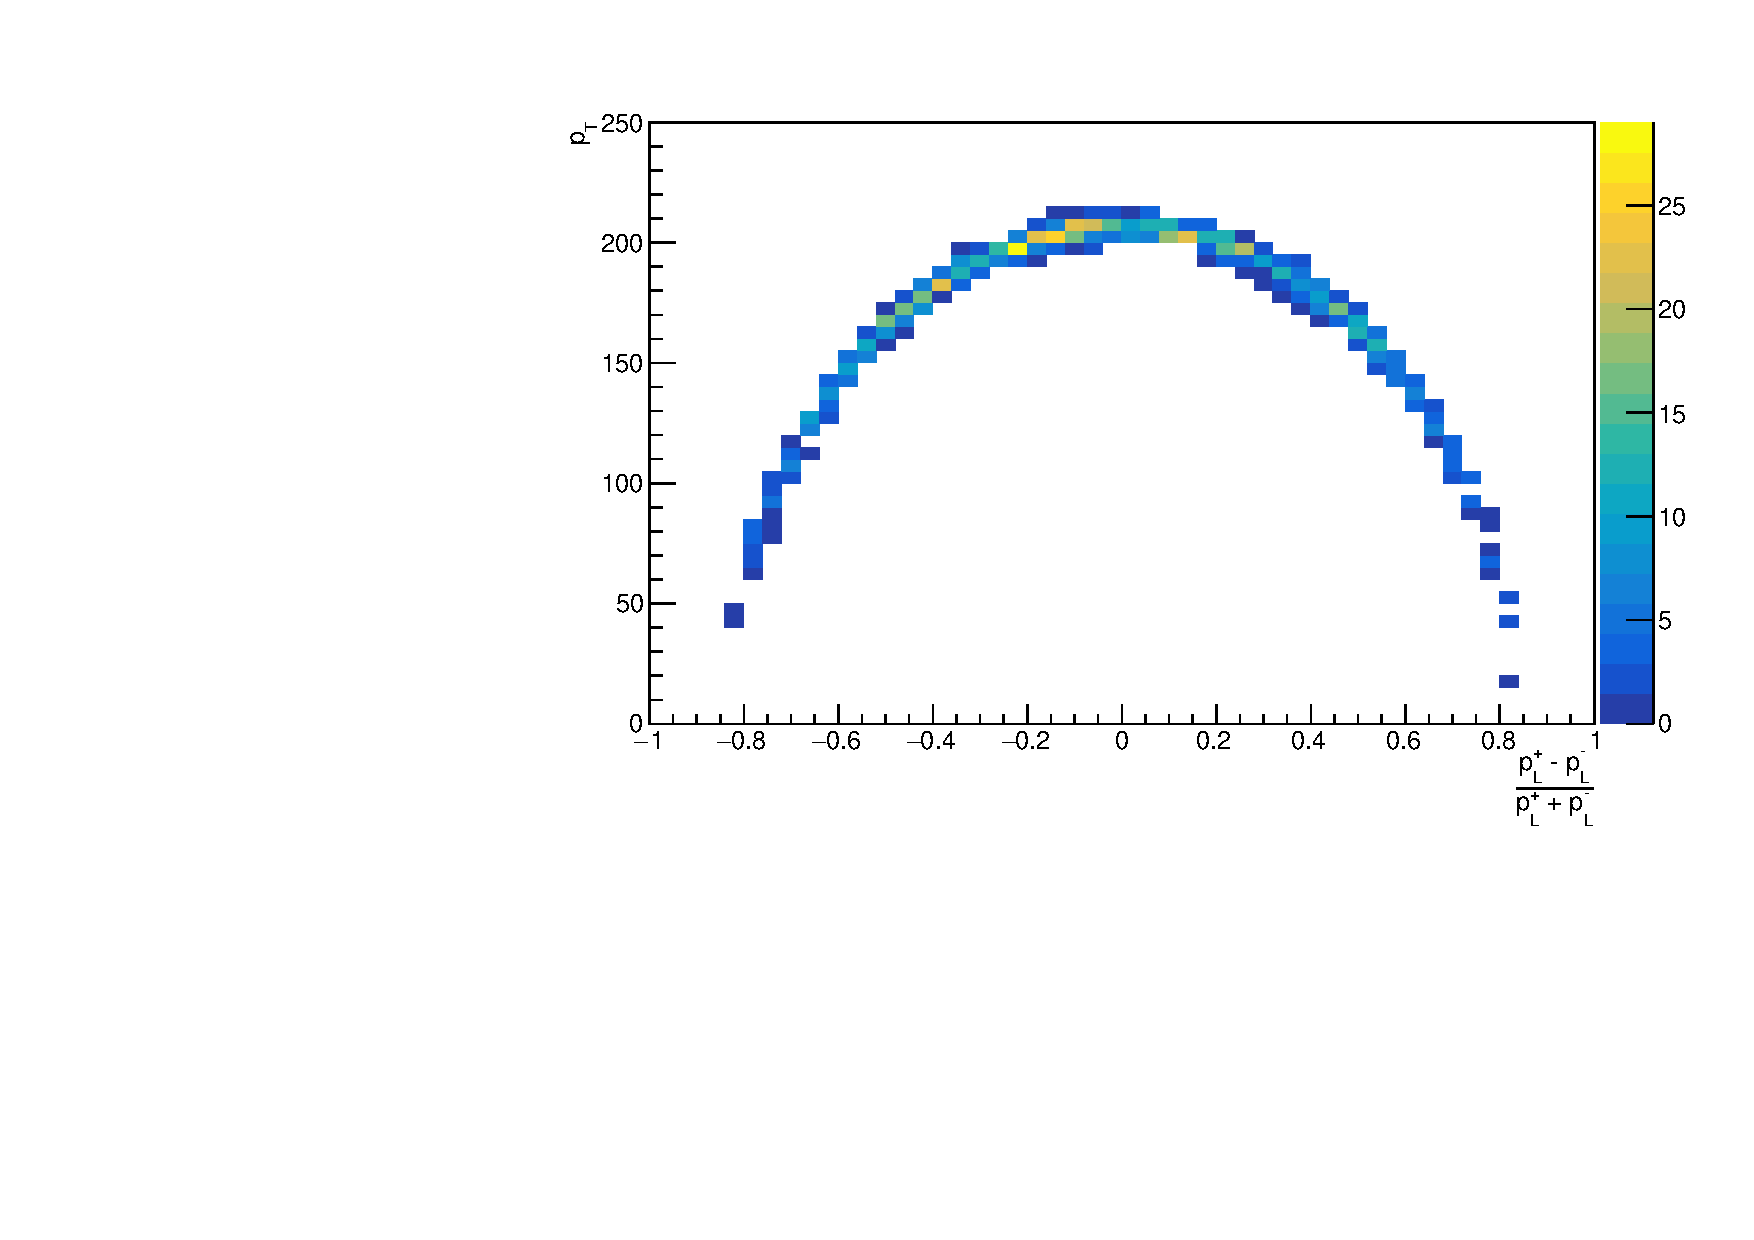
\includegraphics[width=0.5\linewidth]{figures/backgrounds/APplot_dataLL.pdf}
%\put(-190,120) {(a)}
%\hfill
%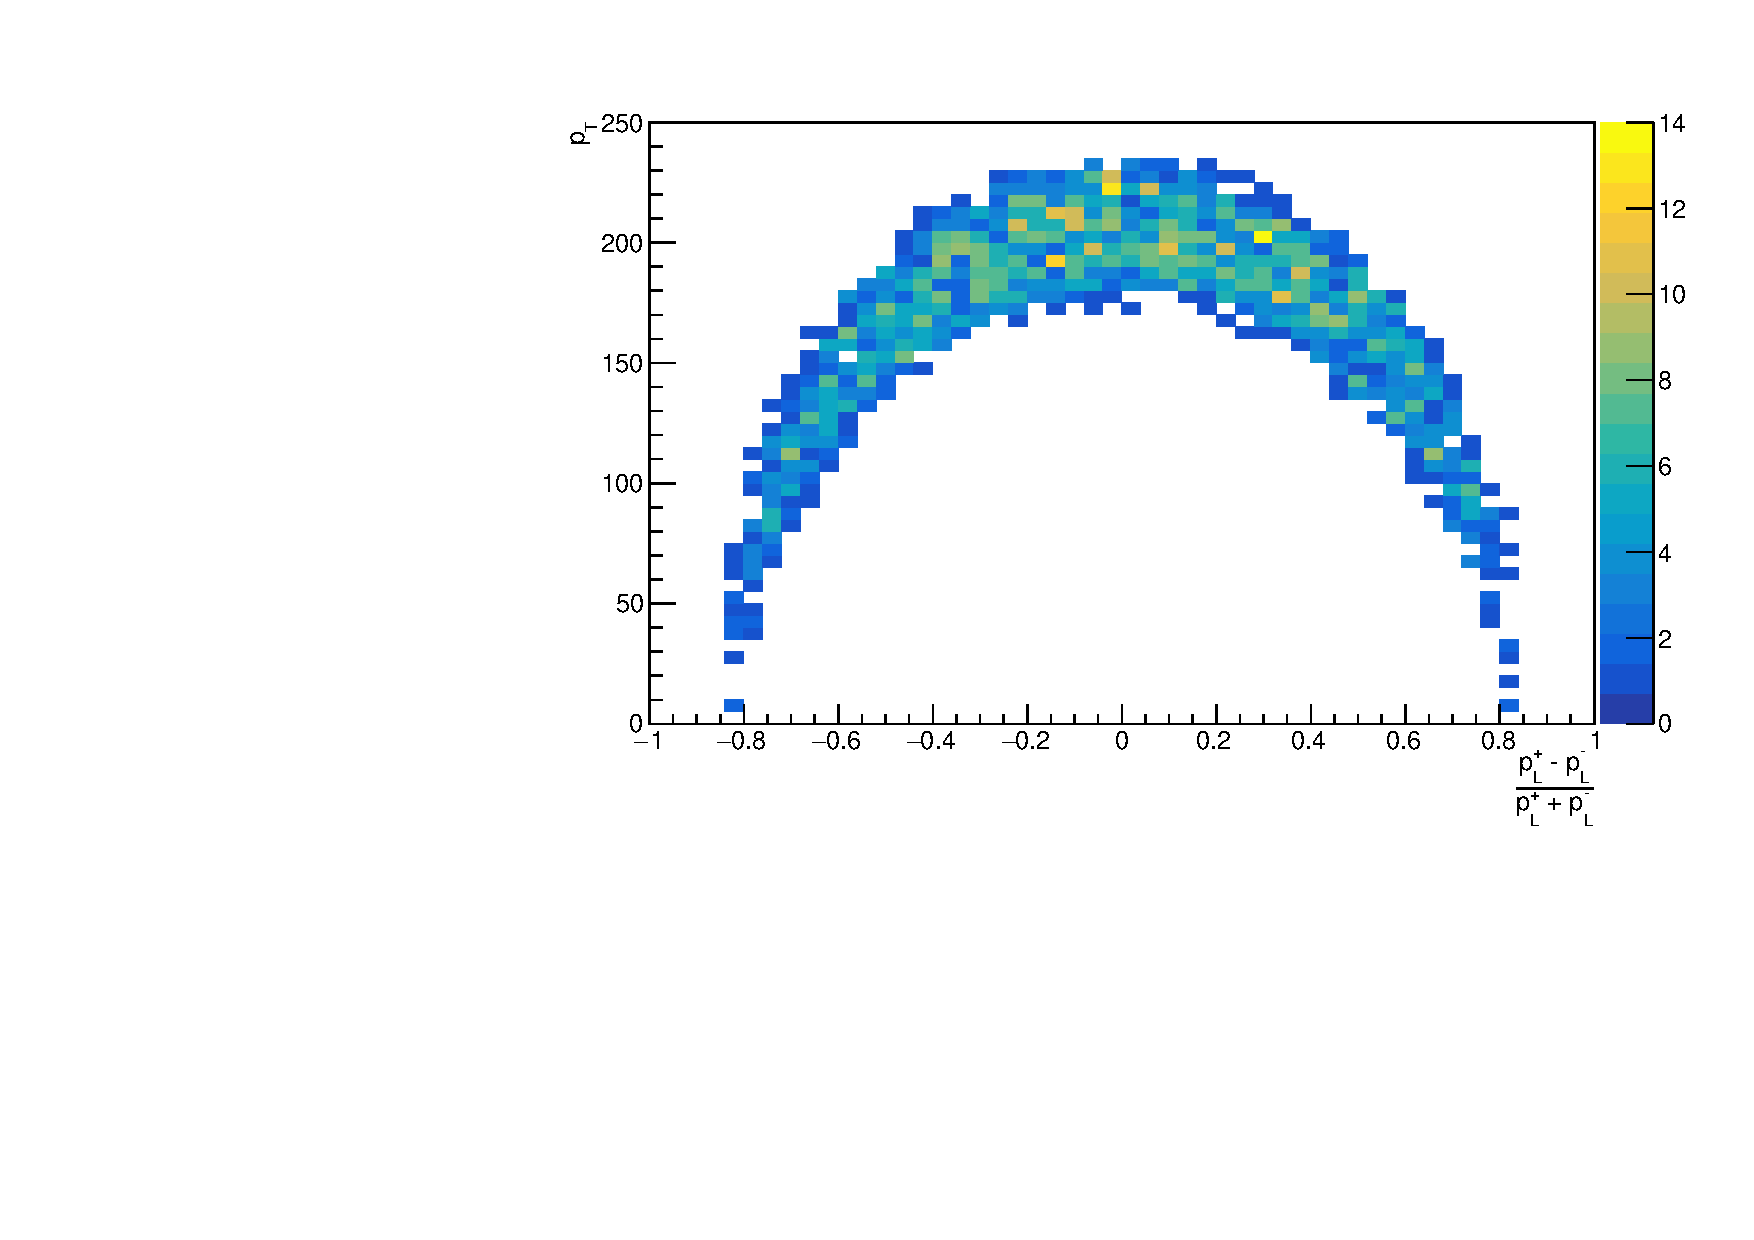
\includegraphics[width=0.5\linewidth]{figures/backgrounds/APplot_dataDD.pdf}
%\put(-190,120) {(b)}
%\caption{Armenteros-Podolanski plots for (a) LL, and (b) DD canididates in data. The $p_T$ values on the y axis are the transverse momentum of the daughters with respect to the mother particle and the x axis contains the longitudinal momentum asymmetry. The black points represent data and the red points represent MC.}
%\label{applotsdata}
%\end{figure}

\begin{figure}
\centering
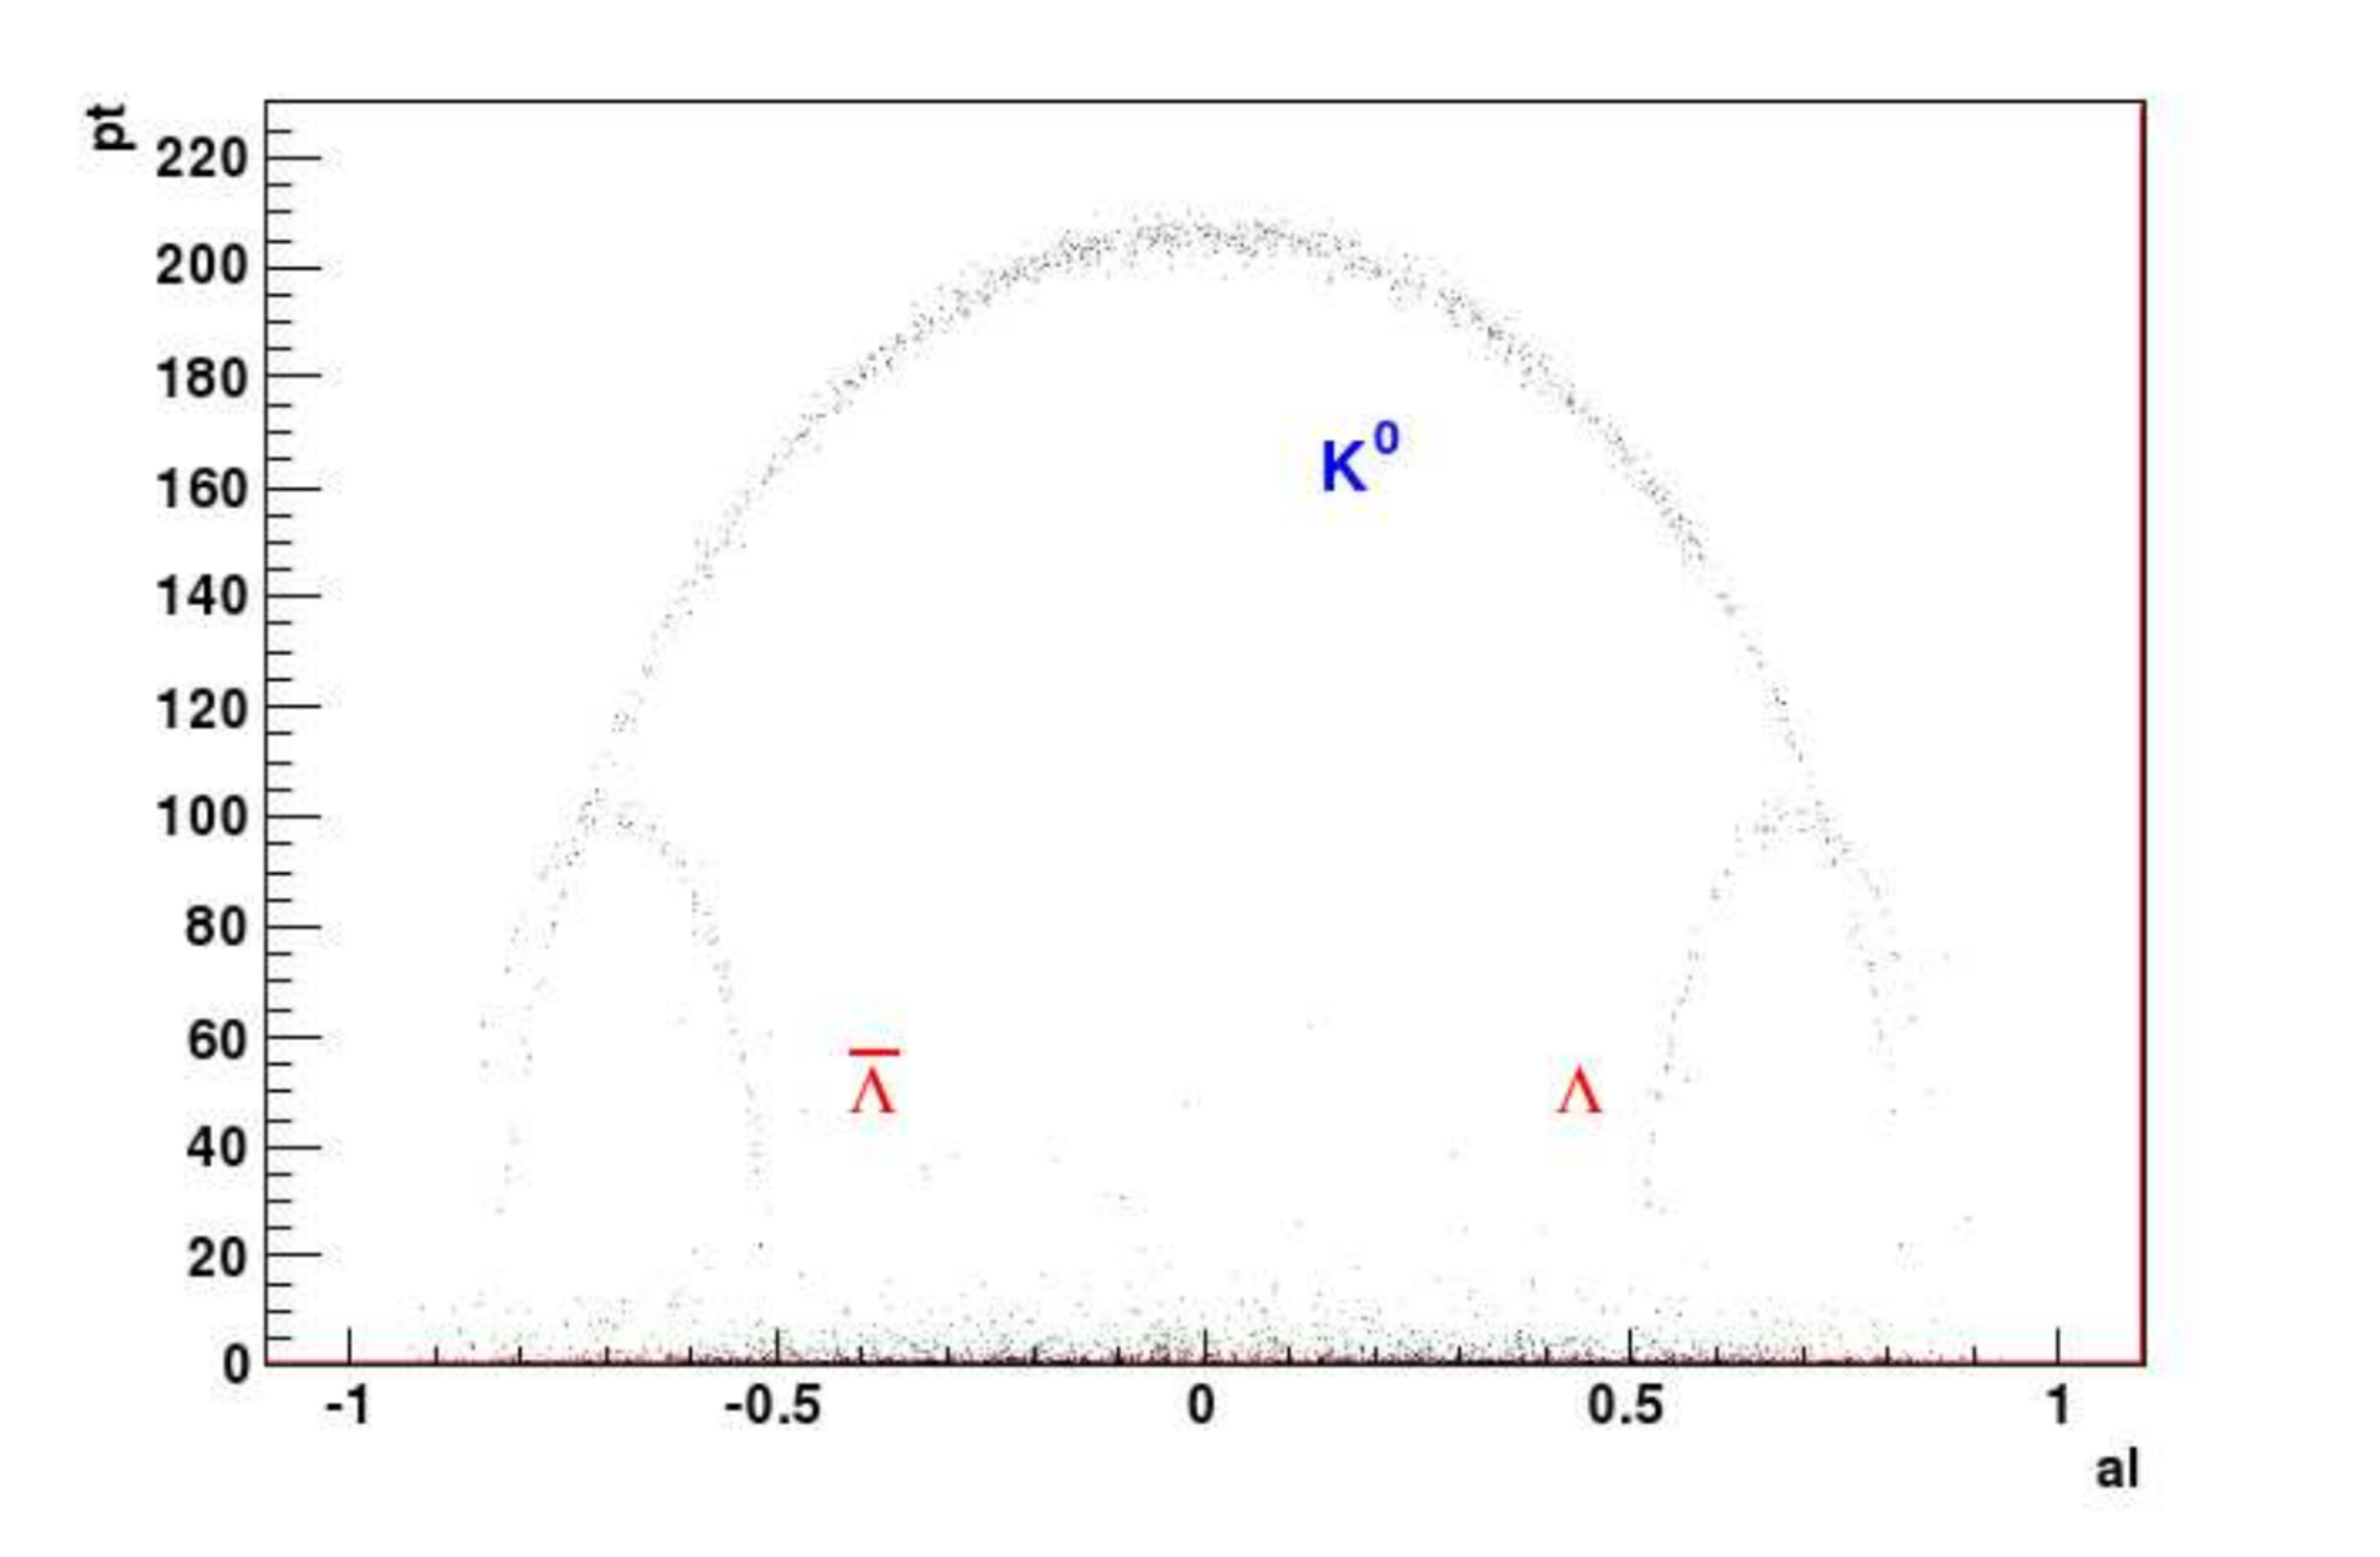
\includegraphics[width=0.5\linewidth]{figures/backgrounds/APfromPaper.pdf}
\caption{An example Armenteros-Podolanski plot showing where the signal regions for \KS, \Lz and \Lbar are located in the AP plane. Reproduced from Ref.~\cite{APplot}.}
\label{apexample}
\end{figure}

\subsubsection{\boldmath \decay{\B}{\D\KS\kaon} background}
\label{sec:backgrounds:b2dkks}

The decay \decay{\Bm}{\D\KS\Km} has a branching fraction of $5.5 \times 10^{-4}$~\cite{PDG2014}, which is similar to the signal \decay{\Bm}{\D\Kstarm(\KS\pim)} branching fraction. However, nearly all of this background is removed by the requirement that the reconstructed \Kstarm mass must be within 75 \mevcc of the known \Kstar mass and the PID requirement on the bachelor pion. The PID requirement on the bachelor pion reduces the rate of misidentification of the bachelor pion, i.e. the efficiency of a \Km passing the bachelor PID requirement, which suppresses the background by about 8\%. The efficiency of the \Kstarm mass selection when applied to the simulated \decay{\Bm}{\D\KS\Km} samples is 3\% for both LL and DD. After accounting for the misidentification rate and selection efficiencies, the expected contribution of \decay{\Bm}{\D\KS\Km} background in the \kpi mass spectrum is less than 1\% of the signal, therefore the decay is considered negligible. Any residual amount is investigated alongside the systematics for the residual low mass background in this region.


%\subsubsection{Other backgrounds}
%
%Other backgrounds have been investigated and shown to have negligible contribution. These decays are investigated by producing simulated samples of background events corressponding to the decay being studied. The selection efficieny of the background is obtained by proccessing the simulated events using \btodkst reconstruction and selection. The expected contribution is estimated using information about the branching ratios of the signal and background decays as well as the efficiency from simulation. By considering the various \B mass distributions in simulation it can be determined if these backgrounds fall within the mass range of interest.
%
%Backgrounds have been investigated and found to be negligible are:
%
%\begin{itemize}
%\item \decay{\Bm}{\Dz\Kstarm\piz}
%\item \decay{\Bs}{\Dz\KS\pip\pim}
%\item \decay{\Bs}{\Dzb\Kstarz(\Kstarp[\pim])}
%\item \decay{\Bs}{\Dstarp\Kstarp}
%\item \decay{\Bs}{\Dspm(\kaon\kaon\pi)\Kstarpm}
%\item \decay{\Bu}{\D\pi} with a random \KS meson added
%\item \decay{\Bd}{\D\KS} with a  random pion added
%\item \decay{\Bs}{\D\KS} with a random pion added
%\item \decay{\Bu}{\D(\KS\pi\pi)\Kp}
%\item \decay{\Lb}{\Lambda_c^-(\proton\Kp[\pim])\Kstarp} with the \proton misidentified as a \Kp meson
%\end{itemize}


\subsection{Particle identification requirements}
\label{sec:selection:pid}

The selection requirements are almost identical for each of the different \Dz modes with the exception of the double misidentification veto applied to the ADS modes. Therefore, it is essential to apply PID selection that efficiently distinguishes between pions and kaons. The PID requirements on the daughters of the \Dz meson are designed so that no \decay{\Dz}{hh'} candidate can appear in more than one category with a change in mass hypothesis. A PID requirement must be made on the bachelor pion to reduce the combinatorial background and remove the \decay{\Bm}{\D\KS\Km} background, discussed in more detail in Section \ref{sec:backgrounds:b2dkks}. The PID requirements for this analysis are listed below:
\begin{itemize}
\item For all \Dz decay modes, the bachelor pion (pion coming from the \Kstarm) is required to satisfy DLLK $<$ 4.
\item For the 2-body \Dz modes the requirements on the \Dz daughters are, kaons must satisfy DLLK $>$ 2 and pions must satifsfy DLLK $<$ -2. 
\item For the \decay{\Dz}{K\pi\pi\pi} modes, e.g. \decay{\Dz}{\Km\pip\pim\pip}, the \Km must satisfy DLLK $>$ 2 and both \pip must satisfy DLLK $<$ -2; no PID requirement is applied for the \pim.
\item For the \decay{\Dz}{\pip\pim\pip\pim}, the two \pip mesons must satisfy DLLK $<$ -2 and no PID requirements are placed on the \pim mesons.
\end{itemize}
%For the bachelor PID (pion coming from the \Kstarm) a requirement of PIDK $<$ 4 is applied. For the 2-body D modes the requirements on the D daughters are kaons must satisfy DLLK $>$ 2 and pions must satifsfy DLLK $<$ -2. For the \decay{\Dz}{K\pi\pi\pi} modes, e.g. \decay{\Dz}{\Km\pip\pim\pip}, the \Km must satisfy DLLK $>$ 2 and both \pip must satifsfy DLLK $<$ -2; no PID requirement is applied for the \pip. For the \decay{\Dz}{\pip\pim\pip\pim}, the two \pip mesons must satisfy DLLK $<$ -2 and no PID requirements is placed on the \pim mesons. 
The PID requirements are the same as those used in the \decay{\Bp}{\D\Kp} analysis~\cite{LHCb-PAPER-2016-003}. No PID requirements are made on the \KS daughters as the high purity of the \KS means that this is not necessary, as shown in Section \ref{sec:backgrounds:contamination}. The efficiency of this PID selection for the \kpi favoured mode in Run 1 is 74\% and the efficiency of \pik events in the favoured mode is 0.15\%; the equivalent \runtwo efficiencies are 82\% and 0.11\% respectively. These efficiencies are discussed in more detail in Section \ref{sec:cpfit:efficiencies:pid}. 

Alternative particle identification variables exist, called ProbNN variables, that assign a value equivalent to a probablity for a given particle being a pion or kaon. These variables are constructed using multivariate analysis techniques. A study into ProbNN variables was undertaken investigating variation of PID efficiencies using different variables and different working points, as shown in Figure \ref{pidoptimisation}. These results show that the DLLK variables outperform the ProbNN variables for this analysis. These results are based on a preliminary version of the selection and so the DLLK efficiencies are not the same as for the final selection. The same PID selection is applied to both Run 1 and Run 2 datasets, as it was found that for the optimised PID selection both PID efficiency and misidentification efficiency were improved for Run 2 compared to Run 1. More detail is given in Section \ref{sec:cpfit:efficiencies:pid}.

\begin{figure}
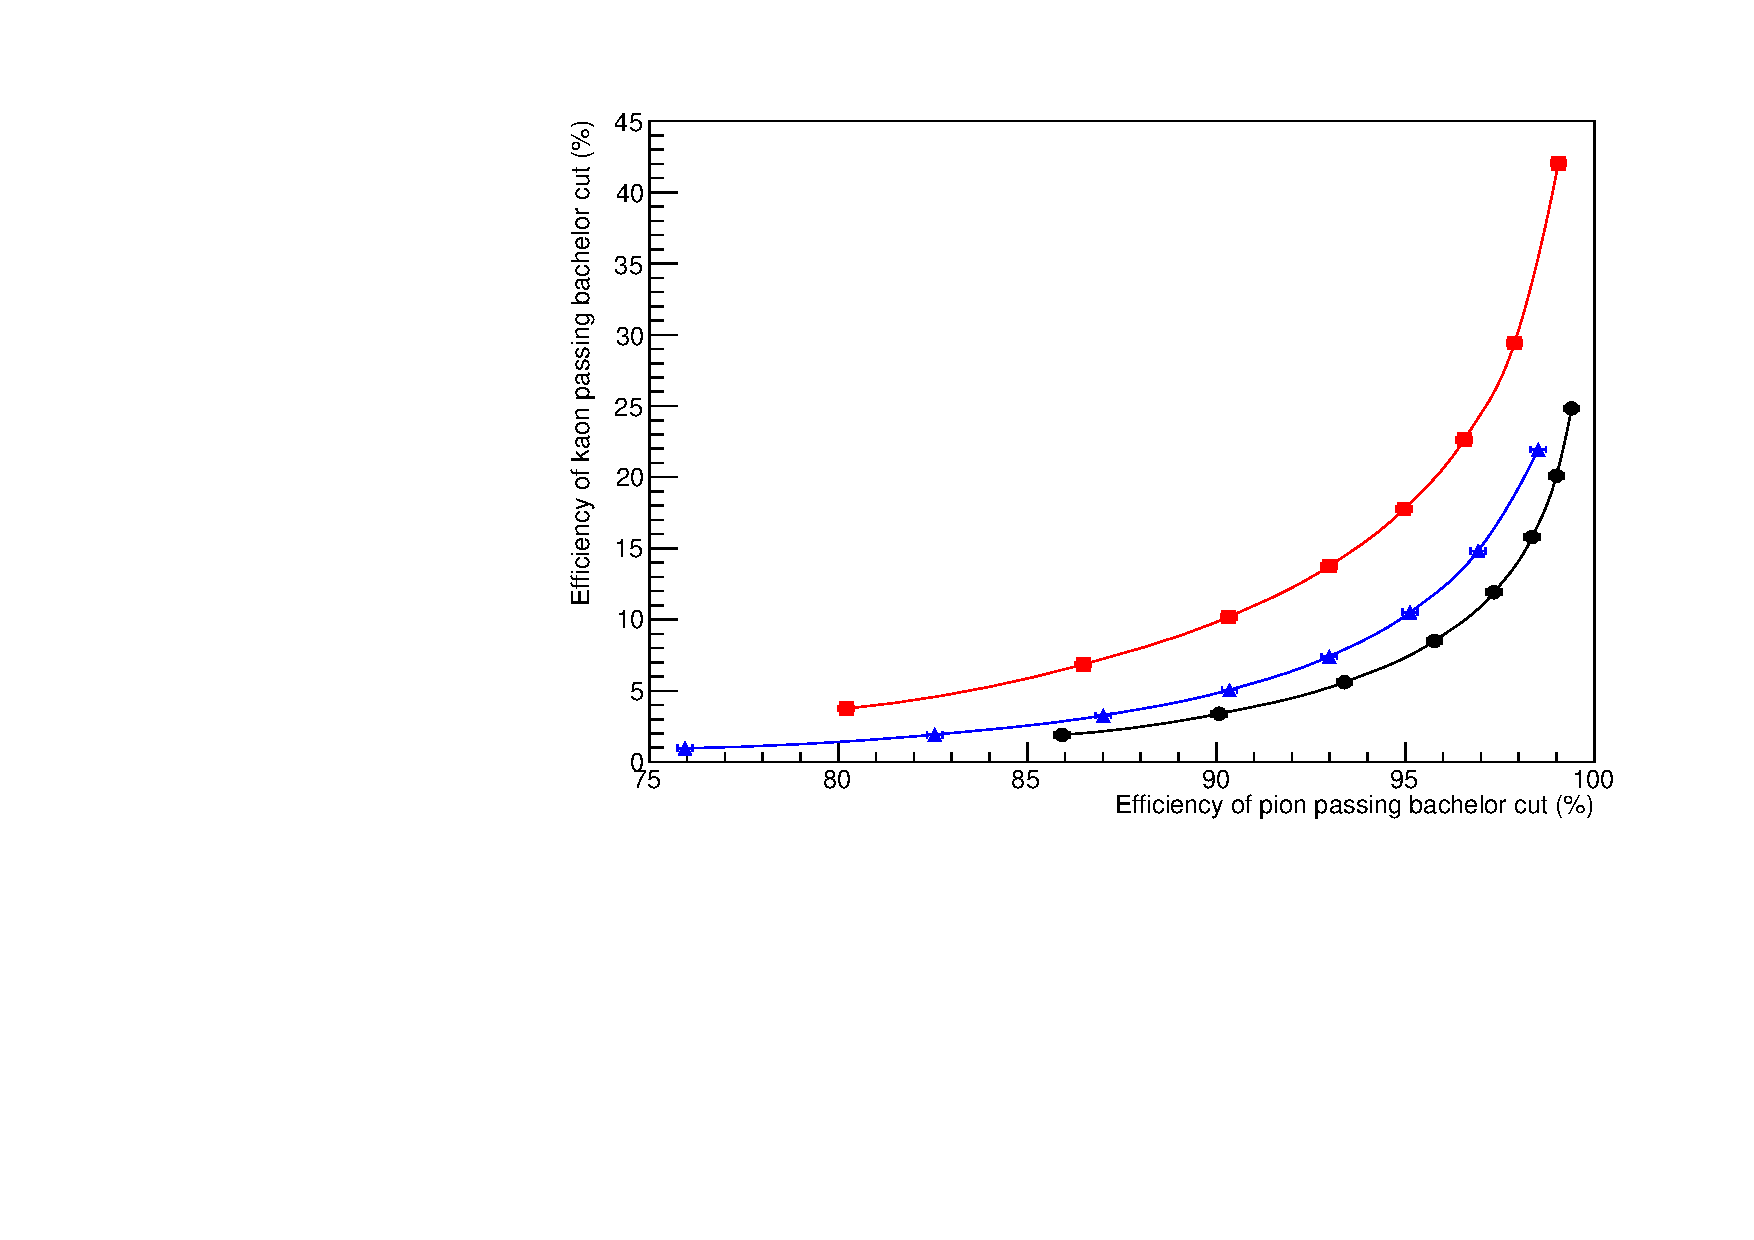
\includegraphics[width=0.5\linewidth]{figures/selection/pidOptimisation_bachelor.pdf}
\put(-150,100) {(a)}
\hfill
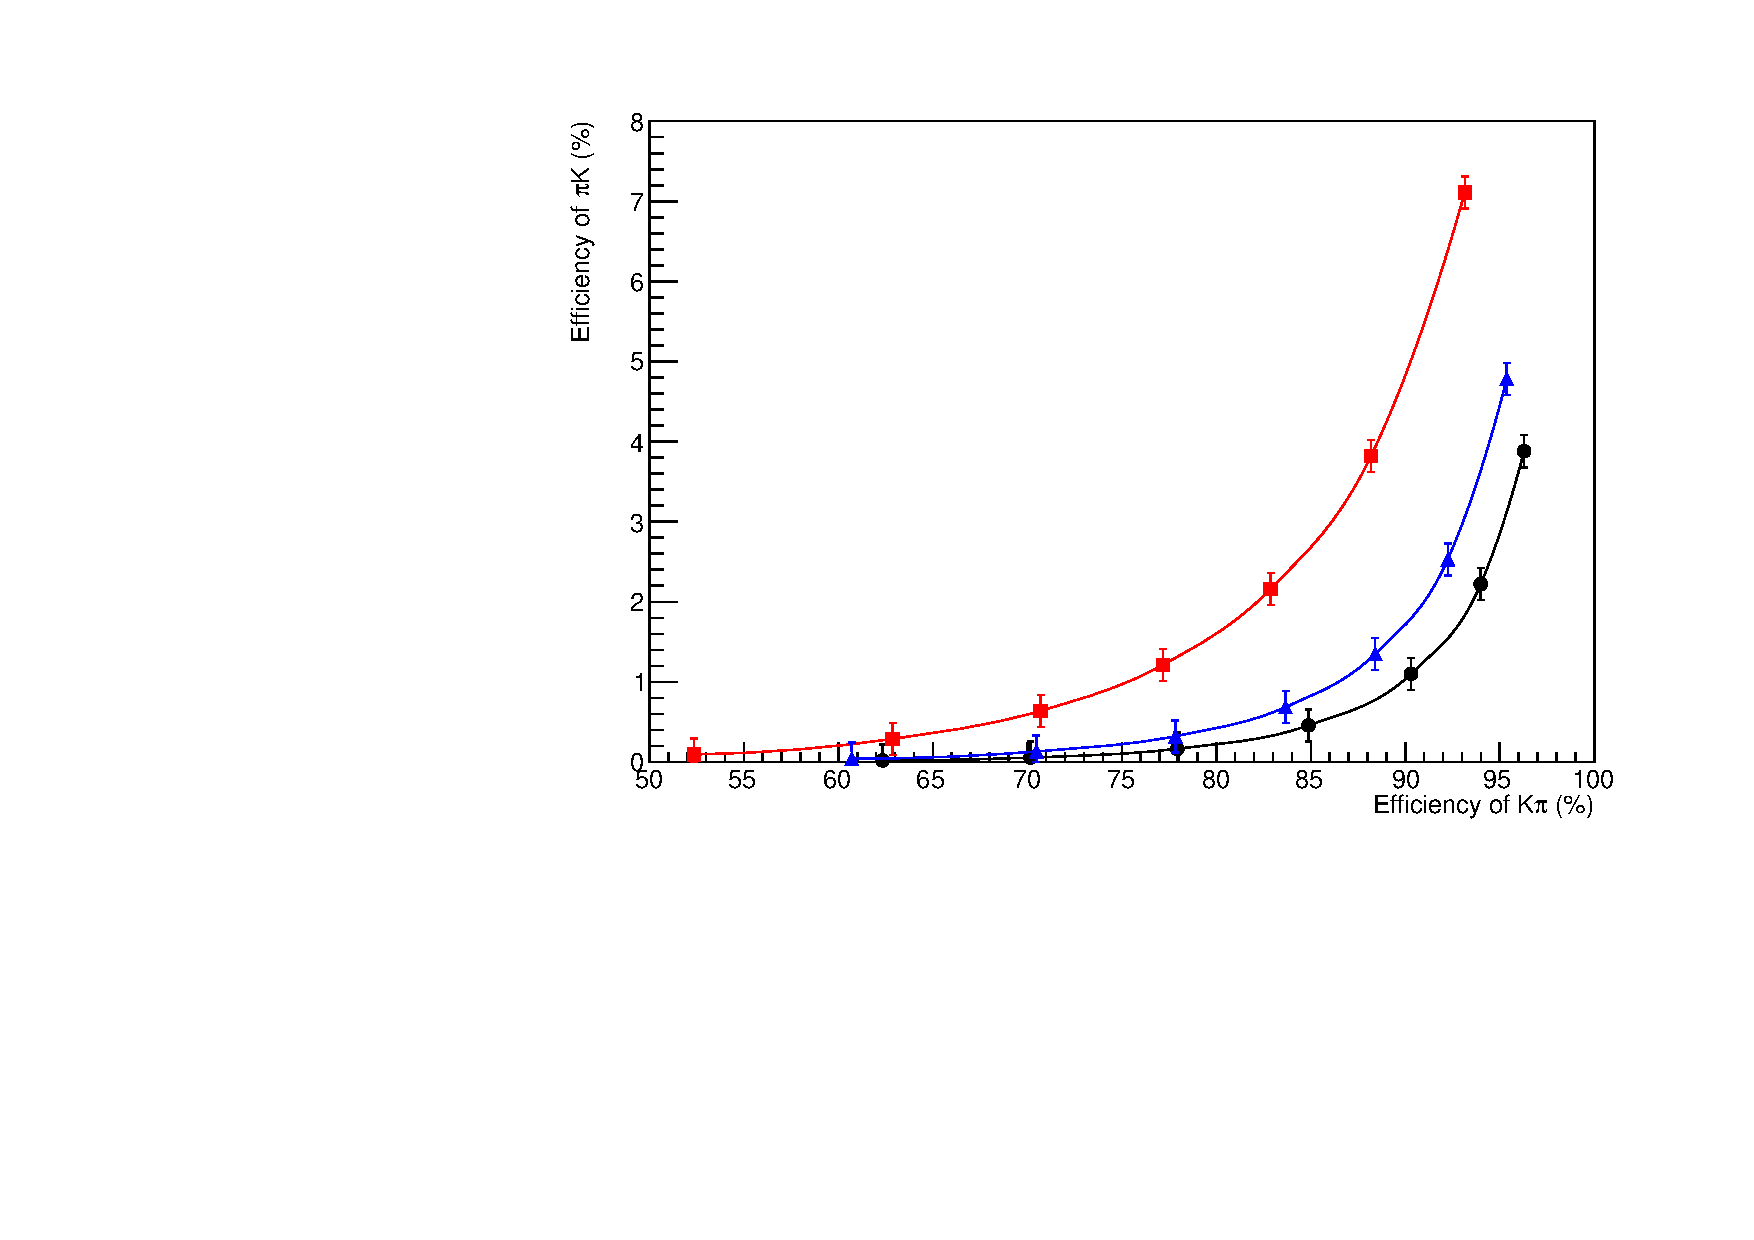
\includegraphics[width=0.5\linewidth]{figures/selection/pidOptimisation_Ddaughters.pdf}
\put(-150,100) {(b)}
\caption{PID efficiencies and misidentification efficiencies using DLLK (black), ProbNNpi (red) and ProbNNpi $\times$ (1-ProbNNk) (blue) for various working points when applied to (a) the bachelor pion, and (b) the D daughters.}
\label{pidoptimisation}
\end{figure}

\subsection{Final refitted \Bm mass distributions}

The refitted \Bm mass distributions of each of the samples passing the full selection requirements, detailed in this chapter, are given in Figure \ref{fig:finalBmass}.

\begin{figure}[h]
\centering
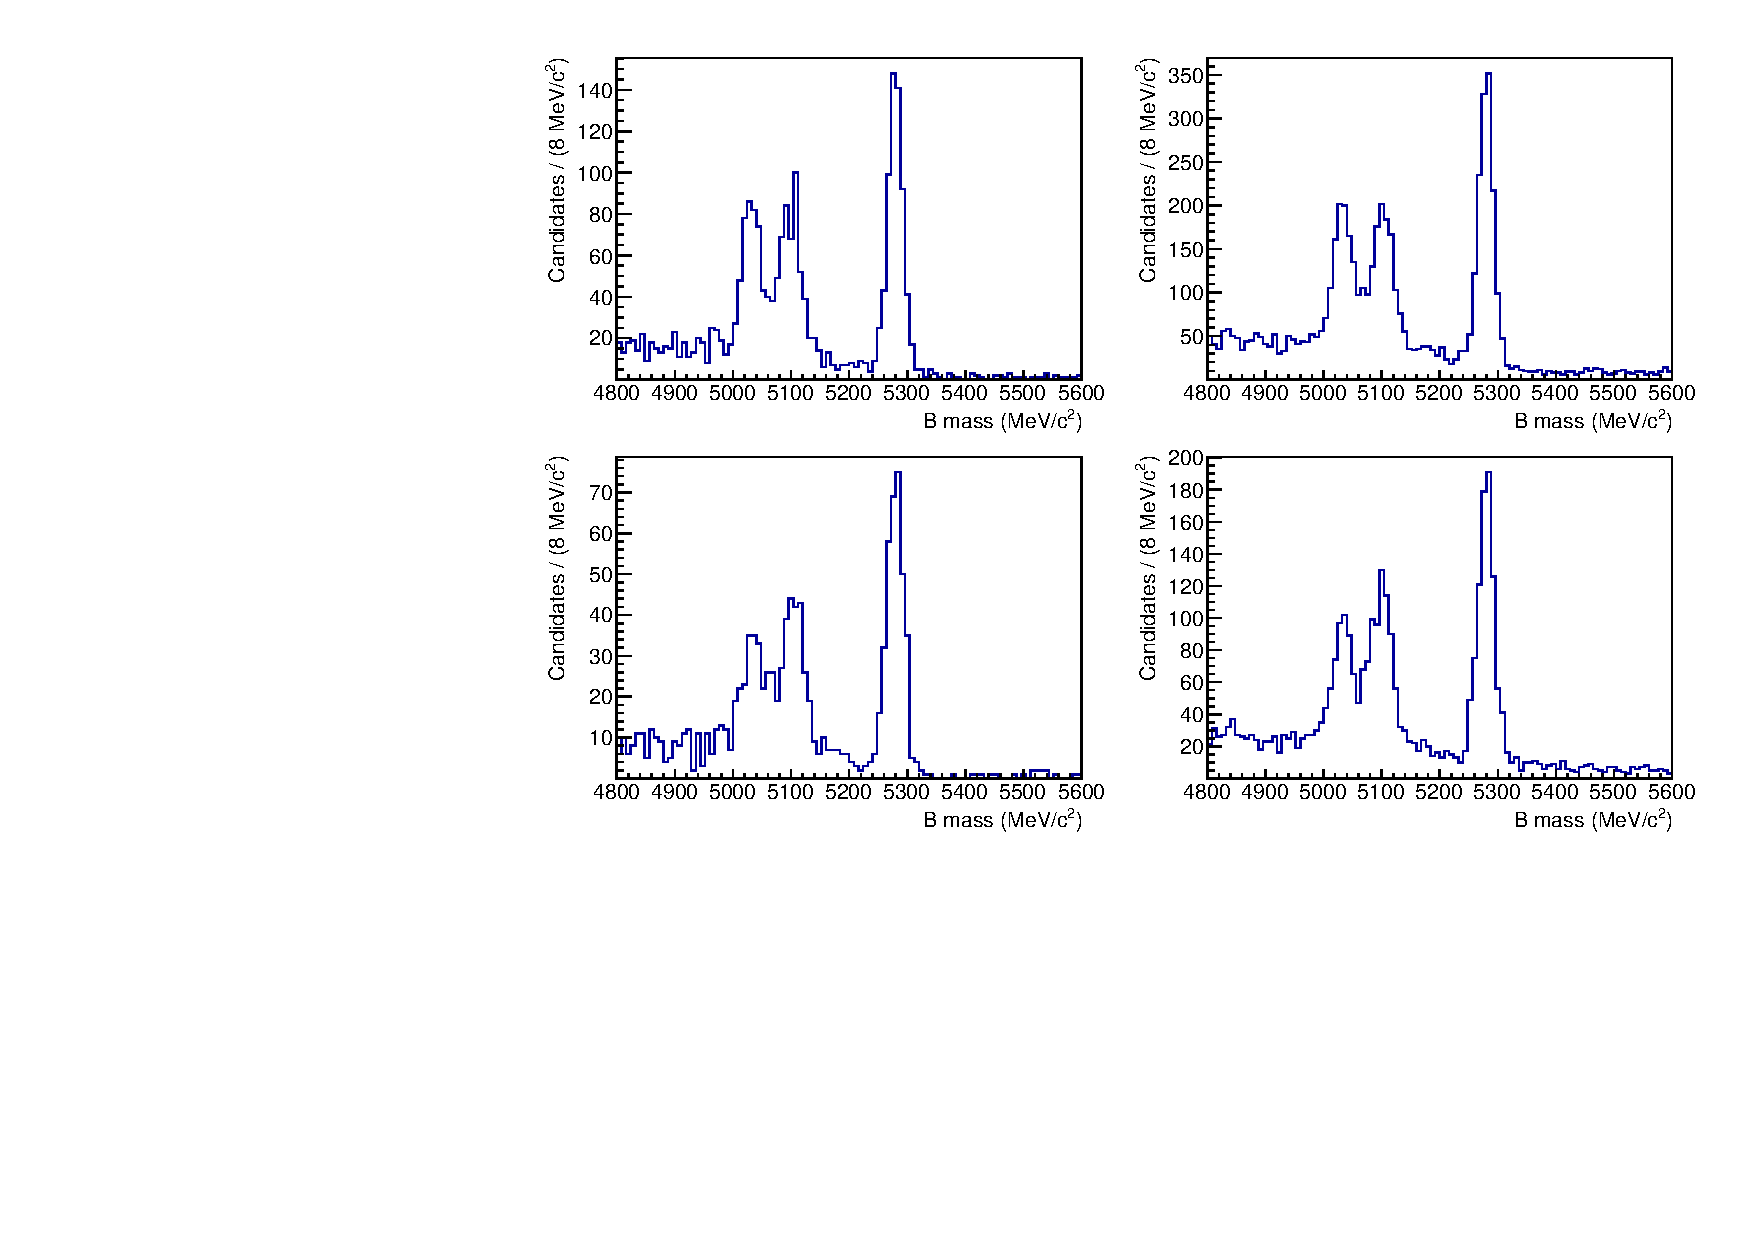
\includegraphics[width=0.8\linewidth]{figures/selection/finalBmass.pdf}
\put(-300,190) {(a)}
\put(-130,190) {(b)}
\put(-300,80) {(c)}
\put(-130,80) {(d)}
\caption{Refitted \Bm mass distributions after the full selection has been applied for (a) \kpi LL, (b) \kpi DD, (c) \kpipipi LL, and (d) \kpipipi DD candidates with \runone and \runtwo samples combined.}
\label{fig:finalBmass}
\end{figure}

\clearpage

\section{Mass parameterisation of the favoured modes}
\label{sec:massfit}

This section describes the mass parameterisation that is developed for the two and four-body favoured \D modes, namely \kpi and \kpipipi. Fits to data are performed on the refitted invariant mass of \Bm candidates. The aim is to develop a model that parameterises the invariant \Bm mass and can then be used in the simultaneous fit described in Section \ref{ch:5-cpfit} to extract the \CP observables. There are three components considered in the model to parameterise the \kpi and \kpipipi \B mass distributions:
\begin{enumerate}
\item Signal, \decay{\Bm}{\D\Kstarm} decays.
\item Combinatoric background, where random tracks are combined in the reconstruction 
\item Partially reconstructed background, where one particle has been missed in the reconstruction, for example \decay{\Bm}{(\decay{\Dstarz}{\Dz[\piz]})\Kstarm}, where the \piz is not reconstructed.
\end{enumerate}

The shape of each fit component, and any constraints in background yields imposed, is discussed in the following sections. The shapes for the LL and DD \KS reconstruction categories are considered separately due to their different reconstructed \Bm mass resolutions.

\subsection{Signal shape}
\label{sec:massfit:signal}

The signal can be described as the sum of two Gaussians each with low mass tails to account for radiative effects. These modified Gaussians are known as Crystal Ball (CB) functions~\cite{Skwarnicki:1986xj}. This Double Crystal Ball shape used is defined by,
\begin{equation}
\mathrm{DCB}(m| \mu,\sigma,\alpha,n,f_{cb}) = f_{cb} \cdot \mathrm{CB}(m| \mu,\sigma,\alpha,n) + (1-f_{cb}) \cdot \mathrm{CB}(m|\mu,f_{\sigma}\sigma,\alpha,n),
\label{DCBshape}
\end{equation}
where
\begin{equation*}
  \mathrm{CB}(m| \mu,\sigma,\alpha,n)=
\begin{cases}
    e^{-((m-\mu)/ \sigma)^2/2},                                   & \text{if } \frac{m-\mu}{\sigma} \geq - \alpha, \\
   \left ( \frac{n}{|\alpha|} \right ) ^n e^{-|\alpha|^2/2} \left ( \frac{n}{|\alpha|} - |\alpha| - \left ( \frac{m-\mu}{\sigma} \right ) \right ) ^{-n} ,    & \text{otherwise.}
\end{cases}
\end{equation*}
where $\mu$ is the peak position, $\sigma$ is the width of the Gaussian, $n$ parameterises the power-law tail, which starts at $\alpha\sigma$ away from the peak position.

Fits to the refitted \B mass distributions have been compared between \runone and \runtwo simulated signal samples, the signal PDFs are shown in Figures \ref{signalfitcomparison2body}. These shapes are consistent between \runone and \runtwo, therefore signal shapes in different data periods are shared in the simultaneous fit. Further comparisons are made between two- and four-body modes. Figure \ref{signalfitcomparisonRun1} compares the signal PDFs obtained from simulated samples between \kpi and \kpipipi for \runone samples. These are significantly different and so \kpi and \kpipipi are associated with different signal shapes in the mass fit.

\begin{figure}[h]
\centering
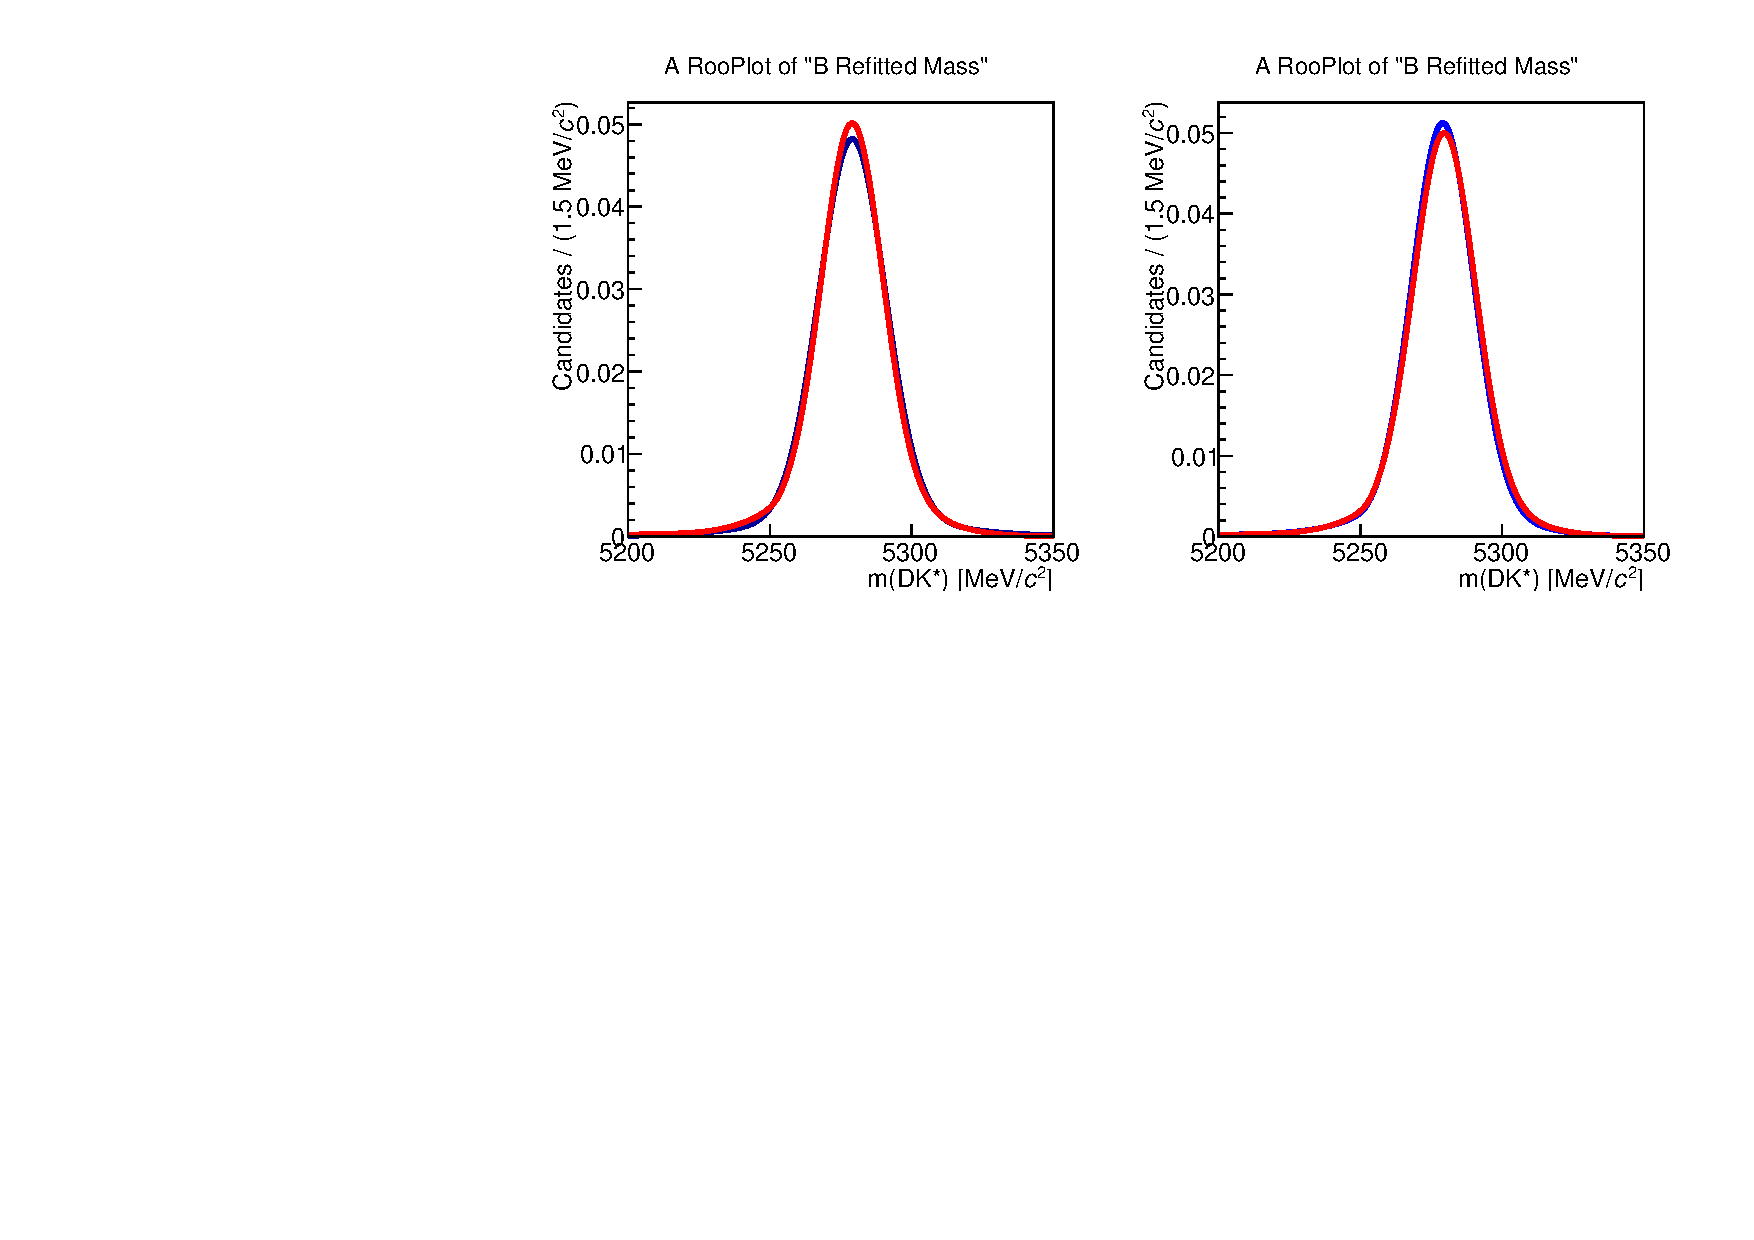
\includegraphics[width=0.7\linewidth]{figures/fitComponents/signalMC_KPi_run1vsrun2.pdf}
\put(-260,100) {(a)}
\put(-110,100) {(b)}
\caption{Comparison of \kpi signal fit functions for \runone (blue) and \runtwo simulated samples (red) for (a) LL candidates and (b) DD candidates}
\label{signalfitcomparison2body}
\end{figure}

\begin{figure}[h]
\centering
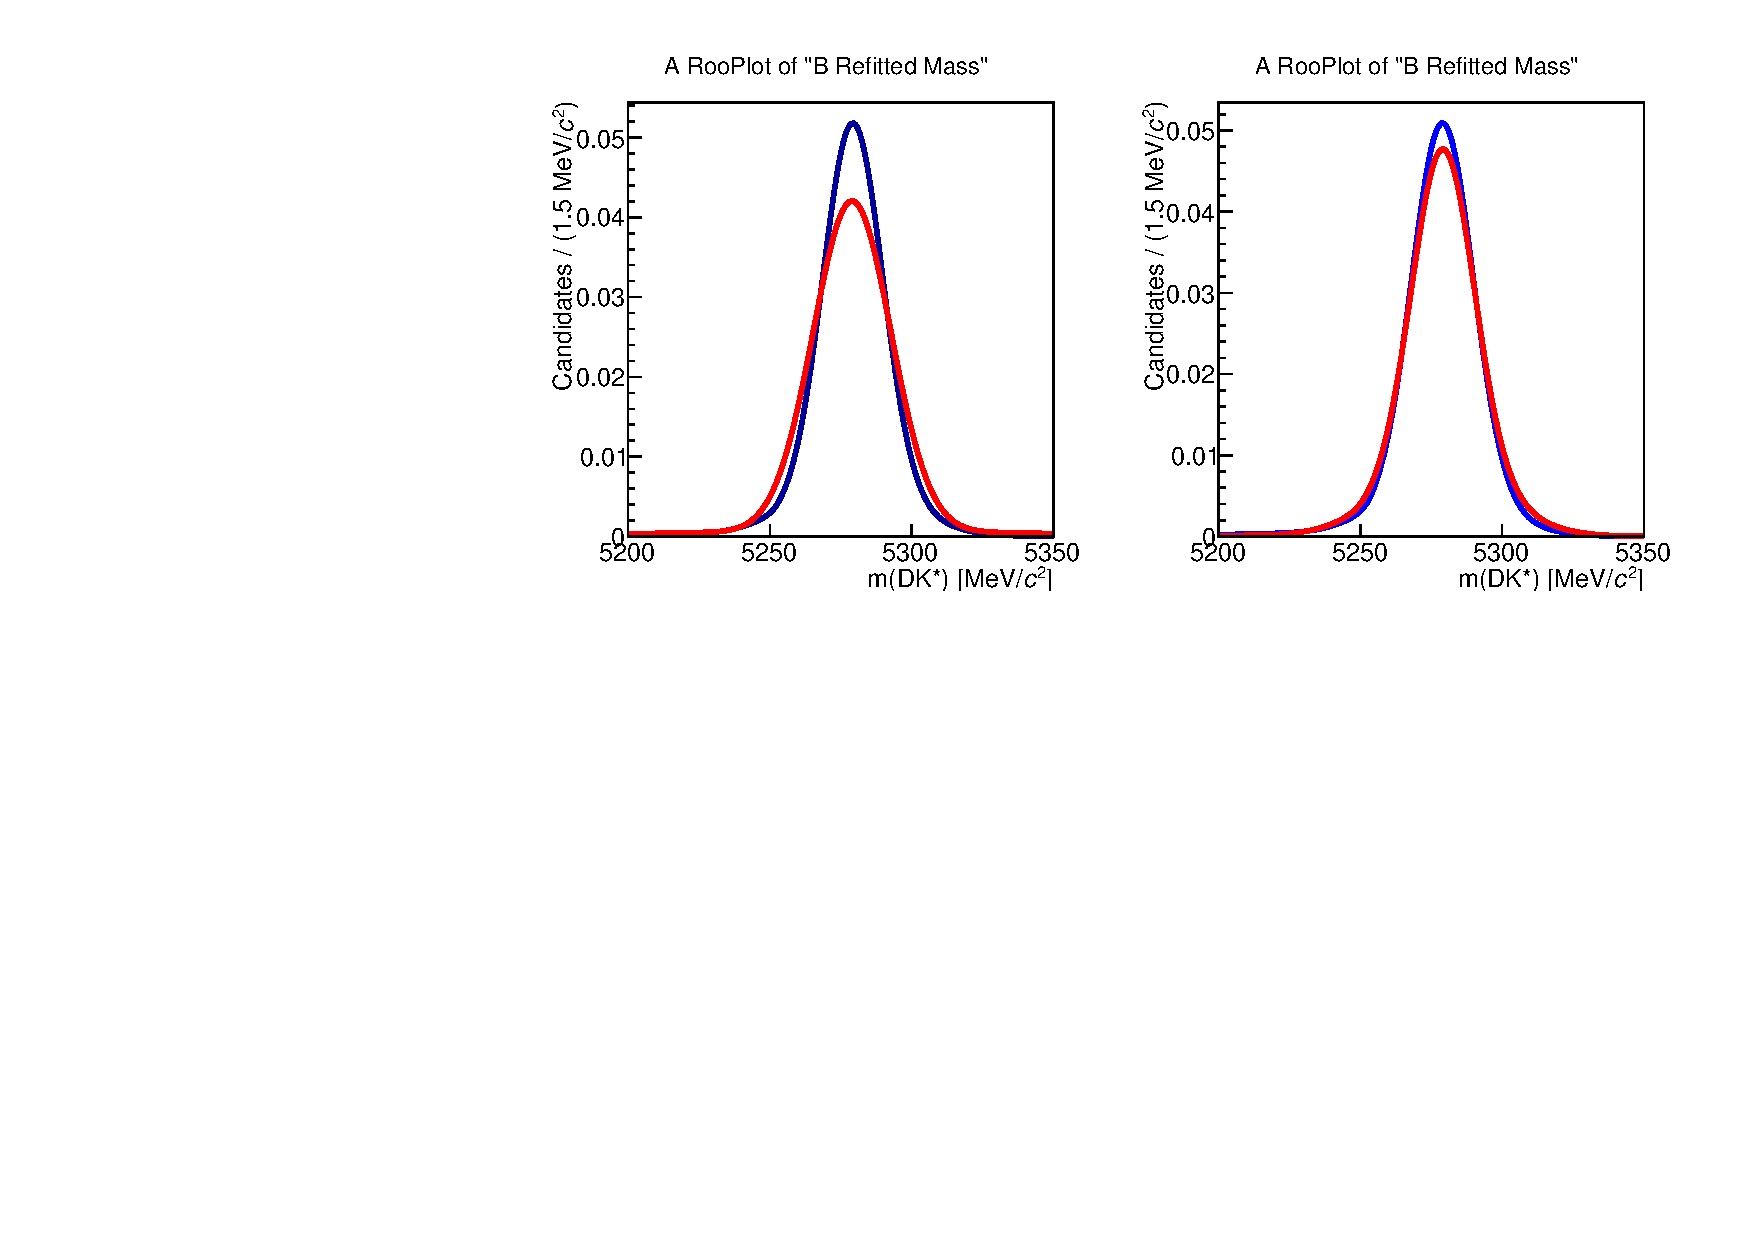
\includegraphics[width=0.7\linewidth]{figures/fitComponents/signalMC_run1_KPivsKPiPiPi.pdf}
\put(-260,100) {(a)}
\put(-110,100) {(b)}
\caption{Comparison of \runone signal fit functions for \kpi (blue) and \kpipipi (red) simulated samples for (a) LL candidates and (b) DD candidates}
\label{signalfitcomparisonRun1}
\end{figure}

For the signal shape in the mass fit, the tail parameters, $\alpha$ and $n$, are fixed from simulation and both CBs share the same peak position and tail parameters.  The width fraction between the CBs, $f_{\sigma}$, is fixed from simulation, but the peak position and width, $\mu$ and $\sigma$, are allowed to vary. The fits to simulated signal samples are shown in Figure \ref{signalfits} and the shape parameters obtained from these fits are detailed in Table \ref{signalparameters}. 

\begin{figure}[h]
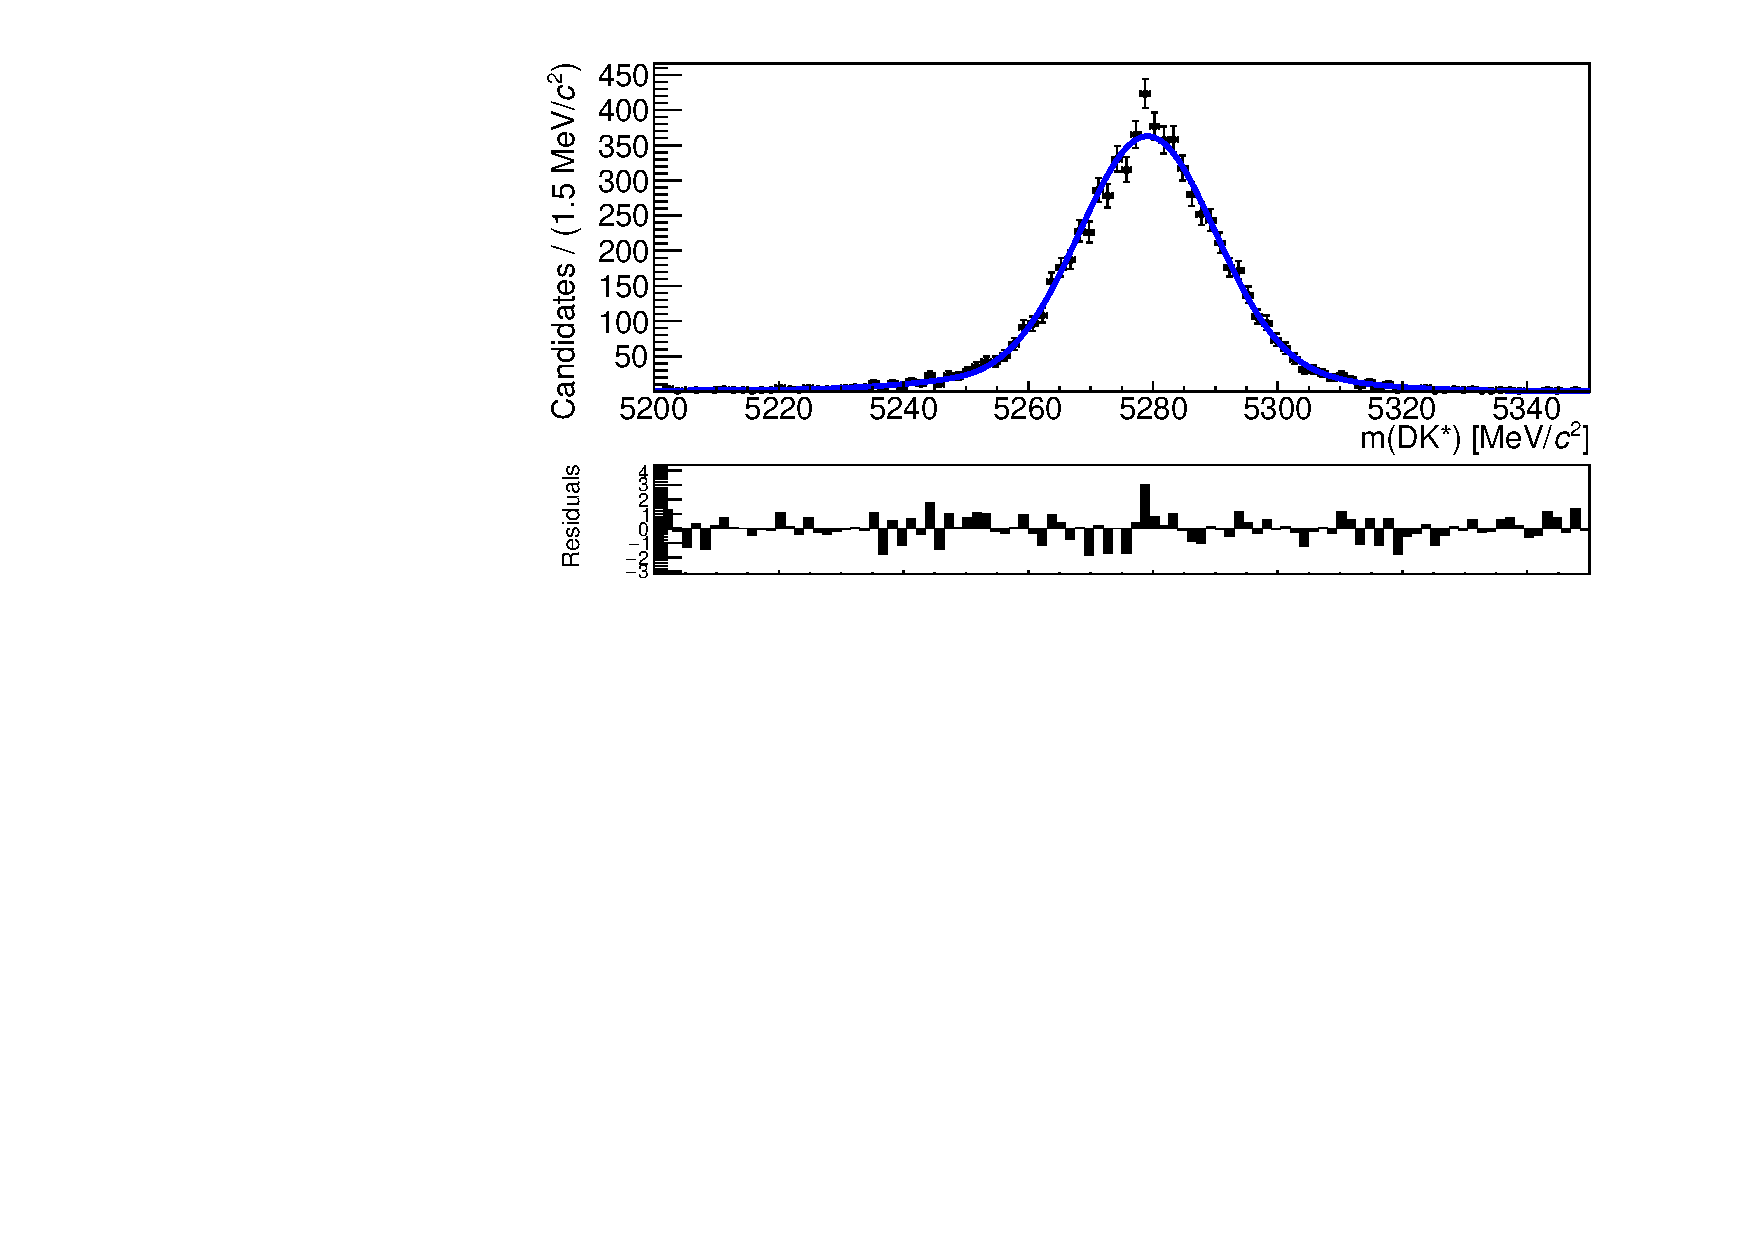
\includegraphics[width=0.5\linewidth]{figures/fitComponents/signalShape_LL_KPi.pdf}
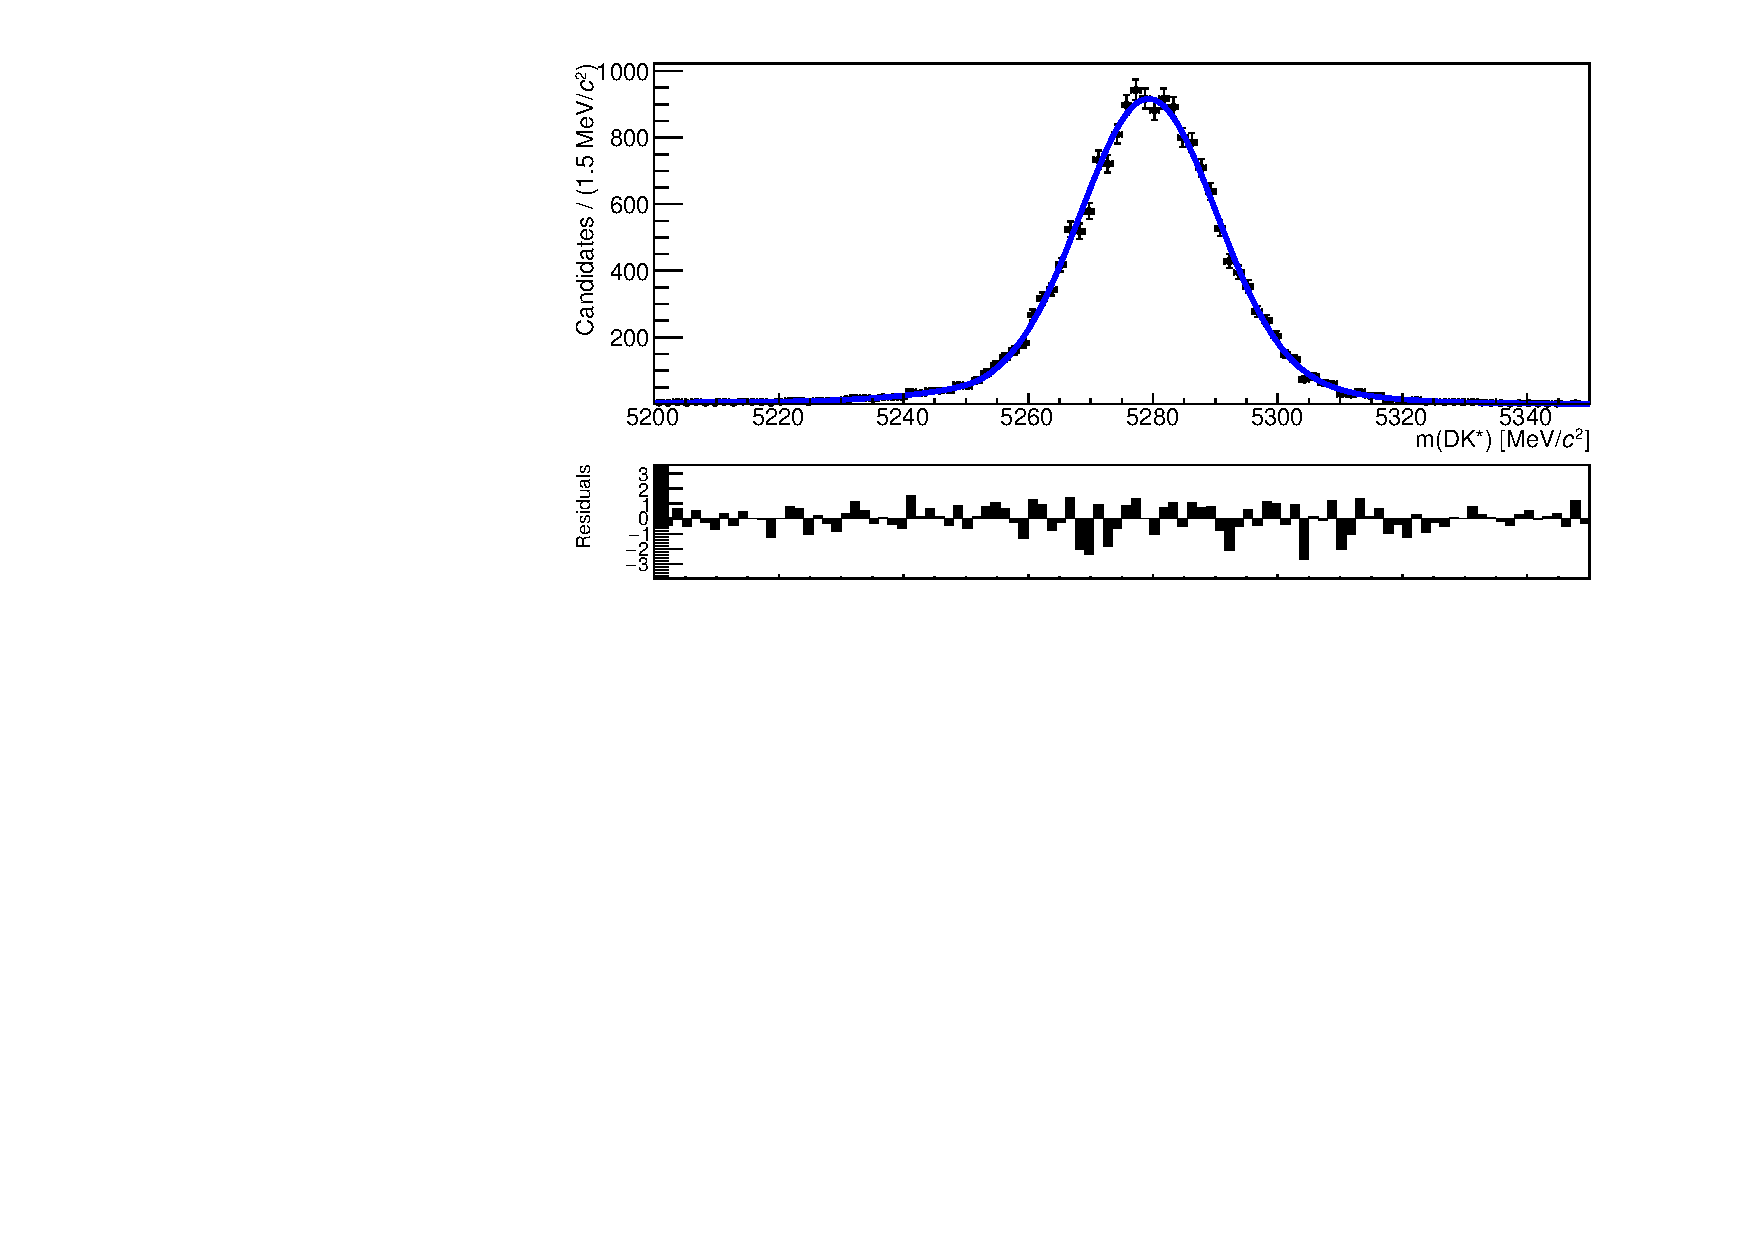
\includegraphics[width=0.5\linewidth]{figures/fitComponents/signalShape_DD_KPi.pdf}
\put(-390,70) {(a)}
\put(-180,70) {(b)}
\hfill
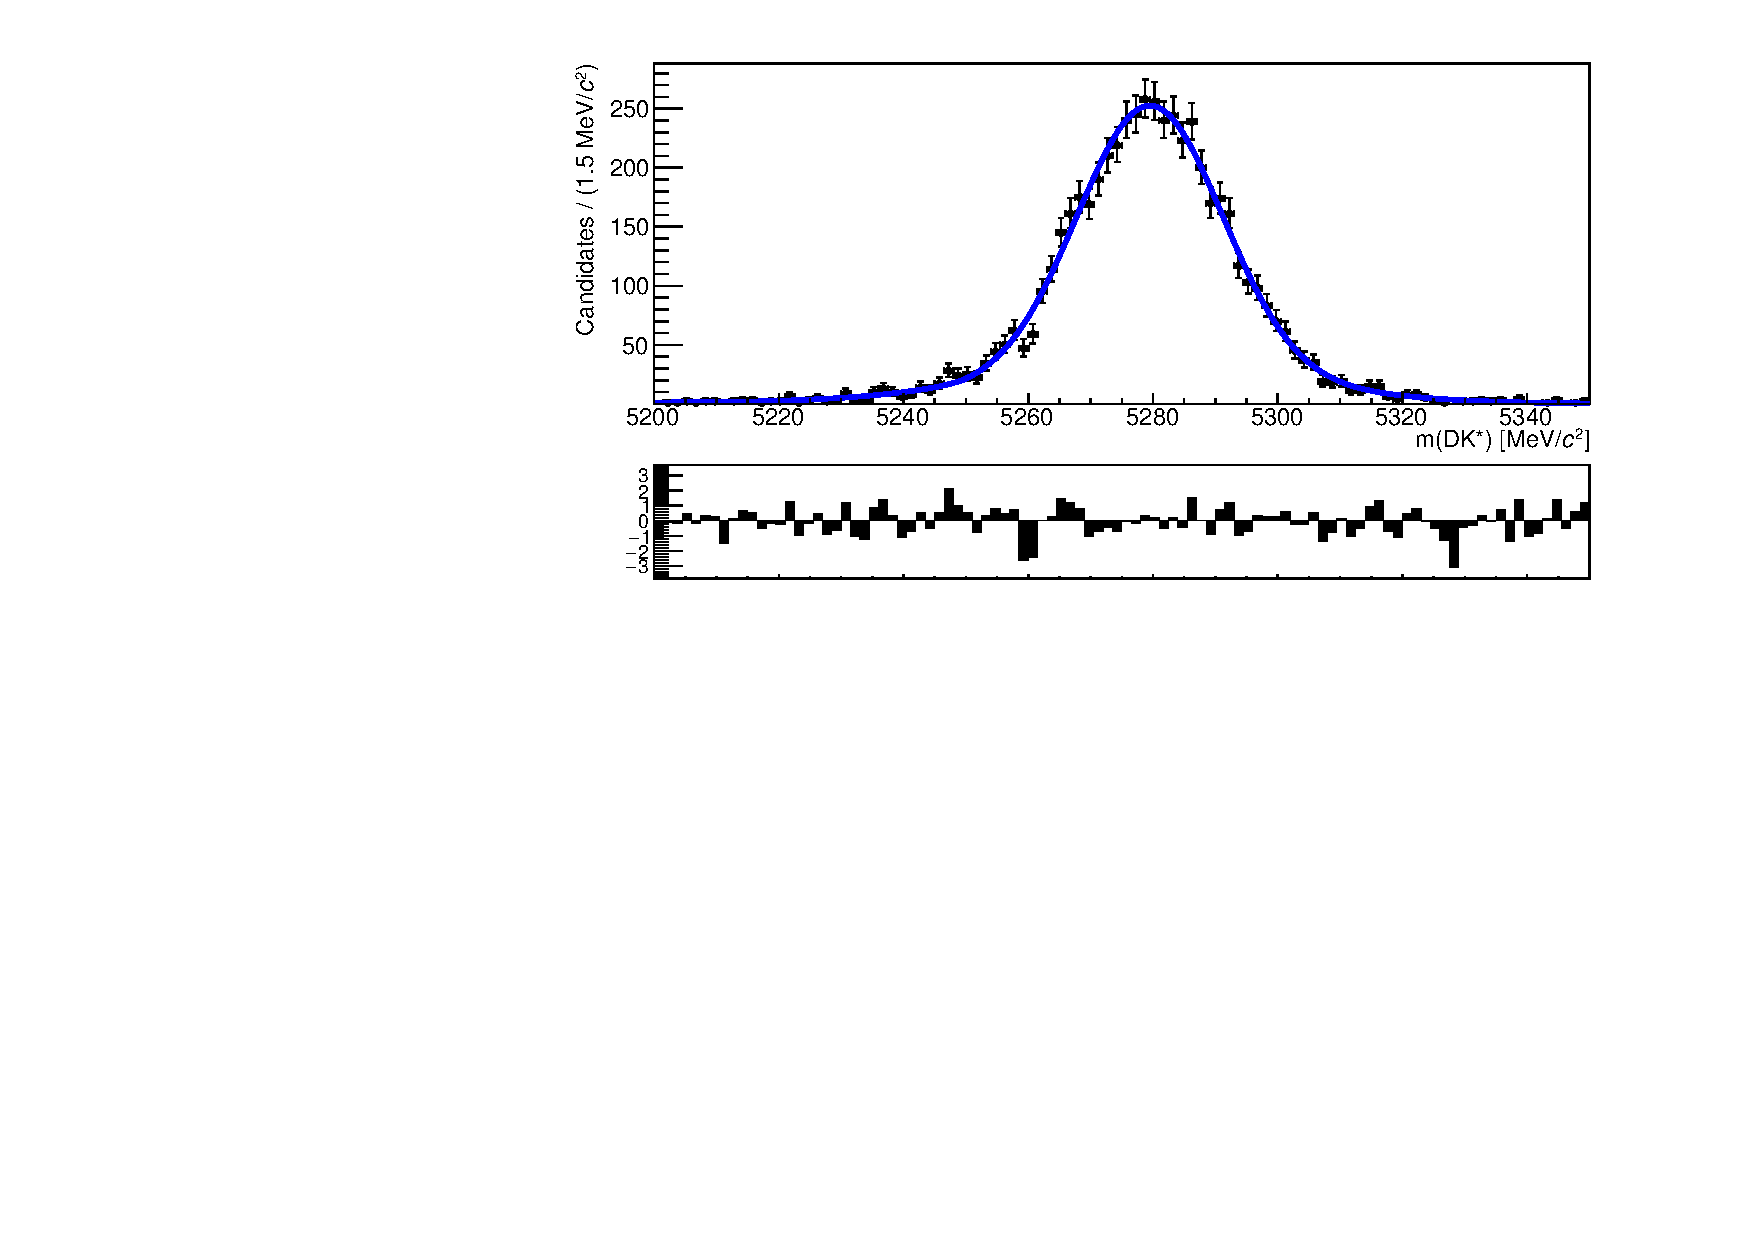
\includegraphics[width=0.5\linewidth]{figures/fitComponents/signalShape_LL_KPiPiPi.pdf}
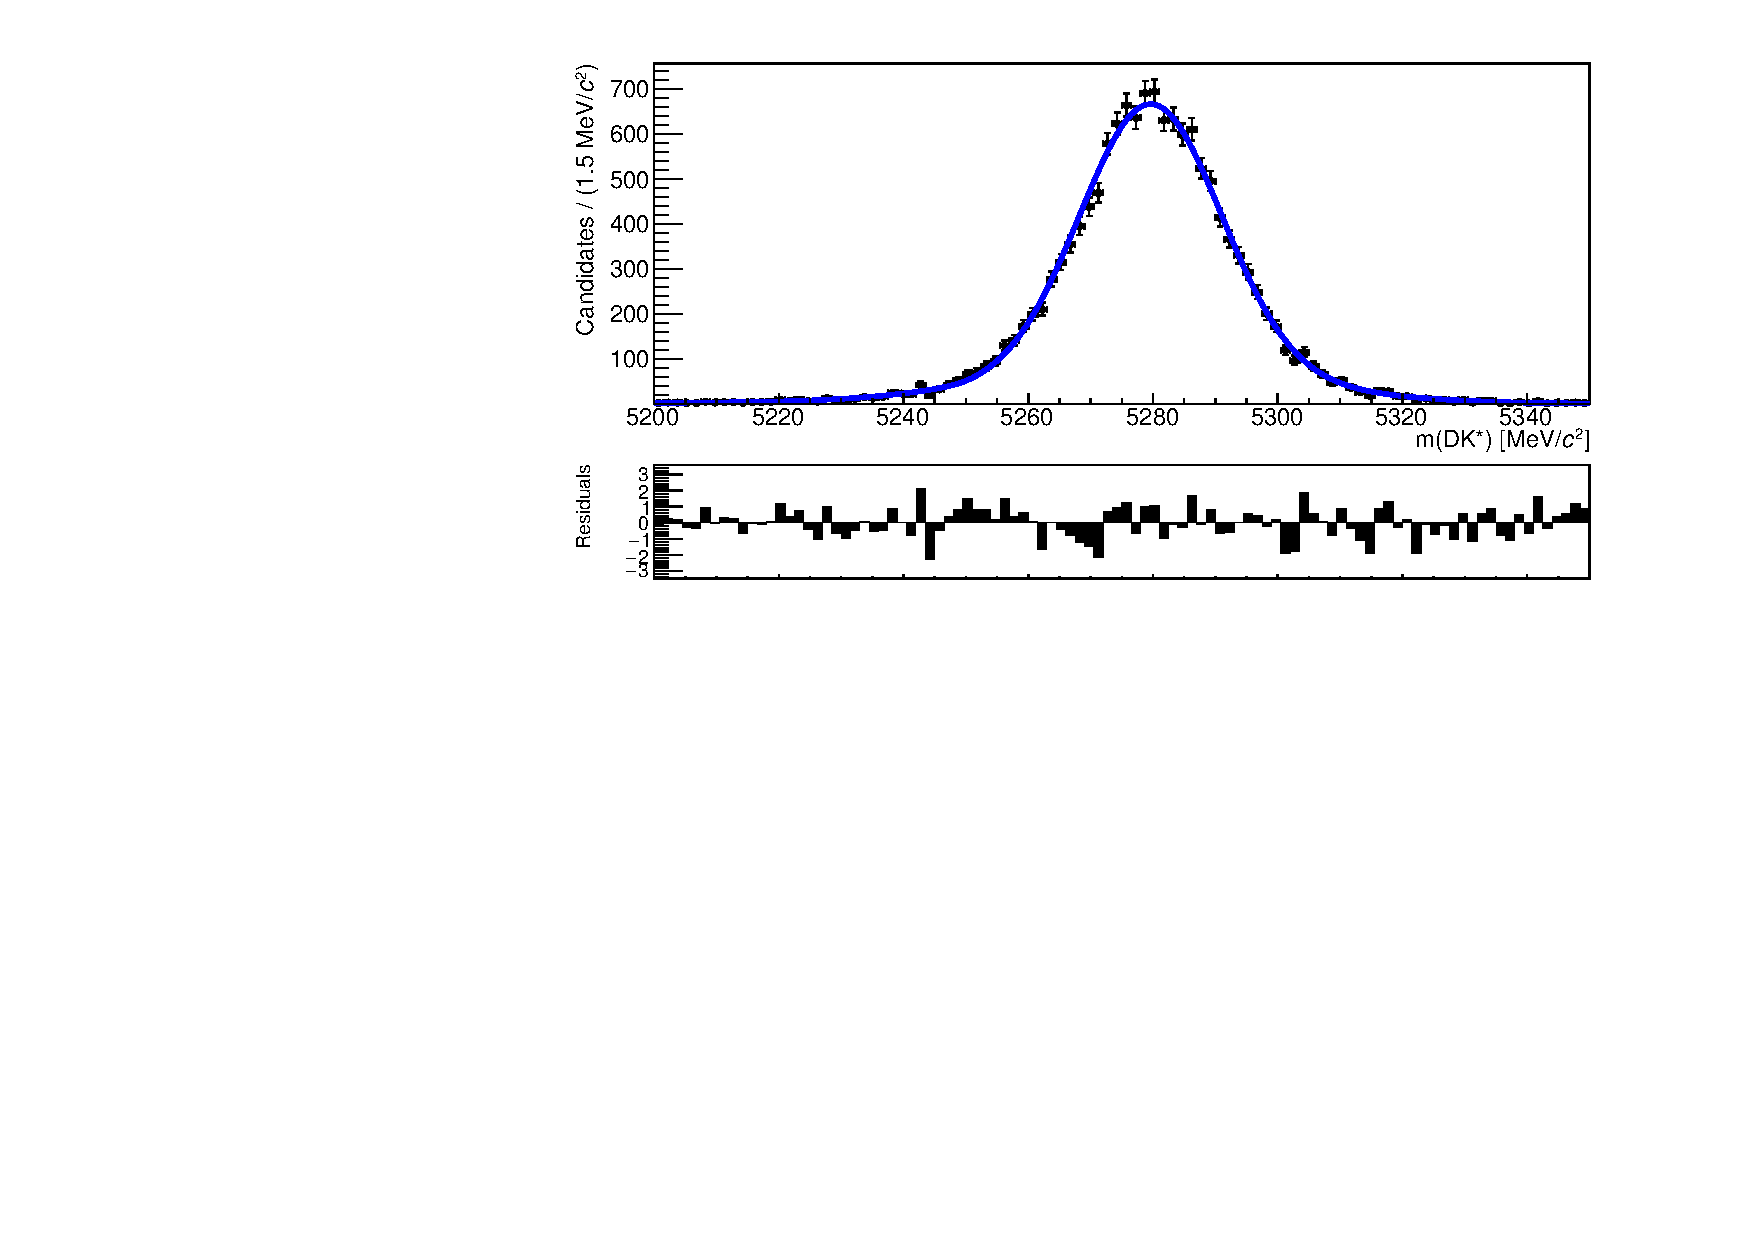
\includegraphics[width=0.5\linewidth]{figures/fitComponents/signalShape_DD_KPiPiPi.pdf}
\put(-390,70) {(c)}
\put(-180,70) {(d)}
\caption{Fits to \runone and \runtwo simulated signal samples combined for (a) \kpi LL, (b) \kpi DD, (c) \kpipipi LL, and (d) \kpipipi DD}
\label{signalfits}
\end{figure}

\begin{table}[h]
\centering
\begin{tabular}{c|cc|cc}
\hline
& \multicolumn{2}{c}{\kpi} & \multicolumn{2}{c}{\kpipipi} \\
& LL & DD & LL & DD\\
\hline
$\mu$ & $5279.12 \pm 0.15$ & $5279.30 \pm 0.09$ & $5279.62 \pm 0.12$ & $5279.50 \pm 0.19$ \\
$\sigma$ & $10.7 \pm 0.3$ & $10.8 \pm 0.2$ & $11.2 \pm 0.2$ & $11.6 \pm 0.3$ \\
$f_{\sigma}$ & $2.04 \pm 0.10$ & $1.97 \pm 0.06$ & $2.08 \pm 0.07$ & $2.10 \pm 0.11$ \\
$\alpha$ & $2.53 \pm 0.07$ & $2.46 \pm 0.04$ & $2.60 \pm 0.07$ & $2.50 \pm 0.10$ \\
$n$ & 1.0 (fixed) & 1.0 (fixed) & 1.0 (fixed) & 1.0 (fixed) \\
$f_{cb}$ & $0.82 \pm 0.03$ & $0.84 \pm 0.02$ & $0.80 \pm 0.03$ & $0.81 \pm 0.04	$ \\
\hline
\end{tabular}
\caption{Signal shape parameters obtained by a fit to \runone and \runtwo simulated signal samples combined for both \kpi and \kpipipi. Parameter names are defined in Equation \ref{DCBshape}. All parameters except for the peak position and width are fixed to these values in the mass fit}
\label{signalparameters}
\end{table}


\subsection{Combinatorial background}
\label{sec:massfit:combinatorial}

The combinatoric background is formed of random tracks that do not correspond to the signal decay, being combined in the reconstruction, for example, random kaon and pion tracks in the detector incorrectly reconstructed to form a \Dz meson. The combinatoric background is modelled using an exponential function, given by $e^{\beta m}$, with a freely floating slope parameter, $\beta$, and yield. The slope parameter is allowed to vary independently in the LL and DD categories and between two and four-body \Dz final states. Each \Dz final state can have a different combinatoric rate.


%%%%%%%%%%%%%%%%%%%%%%
\subsection{Partially reconstructed backgrounds}
\label{sec:massfit:partreco}

Partially reconstructed decays refer to those in which one or more particle has failed to be reconstructed. These decays are parameterised by analytic functions based on a previous studies of \decay{\Bm}{\D\Km}, \decay{\D}{h^+h^-} decays~\cite{LHCb-PAPER-2016-003} and \decay{\Bz}{\D\Kstarz}, \decay{\D}{h^+h^-} decays~\cite{LHCb-PAPER-2016-006}, which have many similar aspects to this analysis.

The partially reconstructed decays are of the form \decay{\B}{\Dstar\Kstar}, where the \Dstar decays to a \Dz meson and a pion or photon that is missed in reconstruction. These backgrounds are observed at a reconstructed invariant mass below the signal peak due to the single particle missed from the invariant mass sum. The \Bm mass range is not large enough to include the case where more than one particle is lost. Three partially reconstructed decays contribute to the invariant mass fit:

\begin{itemize}
\item{\decay{\Bm}{(\decay{\Dstarz}{\Dz[\piz]})\Kstarm}}
\item{\decay{\Bm}{(\decay{\Dstarz}{\Dz[\gamma]})\Kstarm}}
\item{\decay{\Bd}{(\decay{\Dstarp}{\Dz[\pip]})\Kstarm}}
\end{itemize}

where the particle in square brackets corresponds to the missed particle. All of the decay modes listed are modelled using three analytic shapes; RooHORNSdini, RooHILLdini and RooLITTLEHORNSdini, developed by Paolo Gandini and Shu-Faye Cheung. These shapes are physically motivated, exploiting the decay kinematics of partially reconstructed decays.

\decay{\B}{\Dstar\Kstar} is a Scalar $\to$ Vector Vector decay, therefore there are three different helicity amplitudes to consider due to the conservation of angular momentum. Each of these helicity amplitudes produces a \Dstar particle in a different helicity state, labelled +1, 0, -1. The helicity state of the \Dstar and the spin of the missing particle in the subsequent \Dstar decay determines the distribution of the reconstructed \B mass. 

\subsubsection{Horns function}

Consider the \decay{\Bm}{\Dstarz\Kstarm}, \decay{\Dstarz}{\Dz\piz}, where the \Dstarz is in helicity state 0. The helicity of the \Dstarz and the conservation of angular momentum mean that the spin-0 \piz meson will decay predominantly along $\theta = 0^{\circ}$ or $\theta = 180^{\circ}$. When $\theta = 0^{\circ}$, the fraction of momentum carried by the \piz in the \B rest frame is at its smallest, resulting in a larger reconstructed \B mass. Conversely, if $\theta = 180^{\circ}$, the fraction of momentum carried by the \piz is greatest, leading to a lower resonstructed \B mass. The distribution of the helicity angle of the missing particle, $\theta$, has a one-to-one correspondence with its momentum and therefore the reconstructed \B mass. This gives rise to a double peak structure. The \B mass distribution is a parabola, $p_{HORNS}(x)$, with kinematics endpoints $a$ and $b$ where

\begin{align}
p_{HORNS}(x) &= \begin{cases}
\left(x - \frac{a+b}{2}\right)^2, & \text{ if $a \leq x \leq b$}\\ 	
0, & \text{ otherwise.}
\end{cases} 
\end{align}

The parabola is convolved with two Gaussians in order to account for resolution effects. Given a Gaussian function of mean $\mu$ and width $\sigma$, $G(\mu,\sigma)$, a Double Gaussian can be constructed as,

\begin{equation}
DG(x) = f_G G(x|\mu,\sigma) + \left(1-f_G\right) G(x|\mu,R_{\sigma}\sigma) \text{ , }
\end{equation}

where $\sigma$ is the width of the first Gaussian, $f_G$ is the fraction contained by the first gaussian and $R_{\sigma}$ is the relative width between the two. Additionally, selection effects can affect the shape such that one peak is higher than the other. This is taken into account by introducing a linear polynomial with a slope of $1 - \xi$, where $0 \leq \xi \leq 1$. As $\xi \rightarrow 0$, the left hand peak decreases in size relative to the right hand peak. The resulting Horns function is,

\begin{equation}
\text{Horns}(m) = \int_a^b dx \left(x - \frac{a+b}{2}\right)^2 DG(x|m,\sigma,f_G,R_{\sigma}) \left( \frac{1 - \xi_{HORNS}}{b - a}x + \frac{b\xi_{HORNS} - a}{b - a}\right),
\label{eqn:horns}
\end{equation}

where $m$ is the mass variables to be fitted and $x$ is the integration variable in the convolution.

\subsubsection{Hill function}

Consider the \decay{\Bm}{\Dstarz\Kstarm}, \decay{\Dstarz}{\Dz\gamma}, where the \Dstarz is in helicity state 0. The helicity of the \Dstarz and the conservation of angular momentum mean that the spin-1 \Pgamma will decay predominantly along $\theta = 90^{\circ}$ or $\theta = 270^{\circ}$. The fraction of momentum carried by the photon is the same in both of these cases, so not double peak stucture is seen. The resultsing \B mass distribution is a parabola with negative curvature, $p_{HILL}(x)$, and kinematic endpoints $a$ and $b$ where

\begin{align}
p_{HILL}(x) &= \begin{cases}
-(x - a)(x - b), & \text{ if $a \leq x \leq b$}\\ 	
0, & \text{ otherwise.}
\end{cases} 
\end{align}

As with the Horns function, this parabola is convolved with a Double Gaussian and a linear polynomial to account for resolution and selection effects respectively. The resultsing Hill function is,

\begin{equation}
\text{Hill}(m) = \int_a^b dx \left[-(x - a)(x - b)\right] DG(x|m,\sigma,f_G,R_{\sigma}) \left( \frac{1 - \xi_{HILL}}{b - a}x + \frac{b\xi_{HILL} - a}{b - a}\right),
\label{eqn:hill}
\end{equation}

where $m$ is the mass variables to be fitted and $x$ is the integration variable in the convolution.

As the distribution of $\theta$ has a one-to-one correspondence with the reconstructed \B mass, a \Dstar of +1 or -1 would be indistiguishable in \B mass therefore these values are grouped together. This Hill function also applies to the \decay{\Bm}{\Dstarz\Kstarm}, \decay{\Dstarz}{\Dz\piz}, where the \Dstarz is in helicity state $\pm$1.

\subsubsection{Little Horns function}

For the configuration \decay{\Bm}{\Dstarz\Kstarm}, \decay{\Dstarz}{\Dz\gamma}, where the \Dstarz is in helicity state $\pm$1, a third shape is needed, named Little Horns. It is described by a parabola, $p_{LITTLEHORNS}(x)$, and kinematic endpoints $a$ and $b$ where

\begin{align}
p_{LITTLEHORNS}(x) &= \begin{cases}
\left(x - \frac{a+b}{2}\right)^2 + \left(\frac{a-b}{2}\right)^2, & \text{ if $a \leq x \leq b$}\\ 	
0, & \text{ otherwise.}
\end{cases} 
\end{align}

Again, this distribution is convolved with a Double Gaussian and linear polynomial to descibe the resolution and selection effects respectively. This results in a Little Horns function

\begin{multline}
\text{LittleHorns}(m) = \int_a^b dx \biggl\{ \left[ \left( x - \frac{a+b}{2} \right) ^2 + \left( \frac{a-b}{2} \right) ^2 \right] DG(x|m,\sigma,f_G,R_{\sigma}) \\
\left( \frac{1 - \xi_{LITTLEHORNS}}{b - a}x + \frac{b\xi_{LITTLEHORNS} - a}{b - a} \right) \biggr\}
\label{eqn:littlehorns}
\end{multline}

\subsubsection{Total partially reconstructed function}

Table \ref{helicityamplitudes} summarises the uses of the different analytic shapes described: Horns, Hill and Little Horns functions. In order to obtain values for the various parameters in these shapes simulated events were generated and the full reconstruction and selection was applied, except for the PID selection. Comparisons between \runone and \runtwo simulated events for partially reconstructed decays are shown in Figure \ref{parterecofits}. These distributions are considered sufficienctly similar to fix the shapes across all years. The parameters for the partially reconstructed shapes are obtained from performing individual fits to \runone simulated samples.

\begin{figure}[!h]
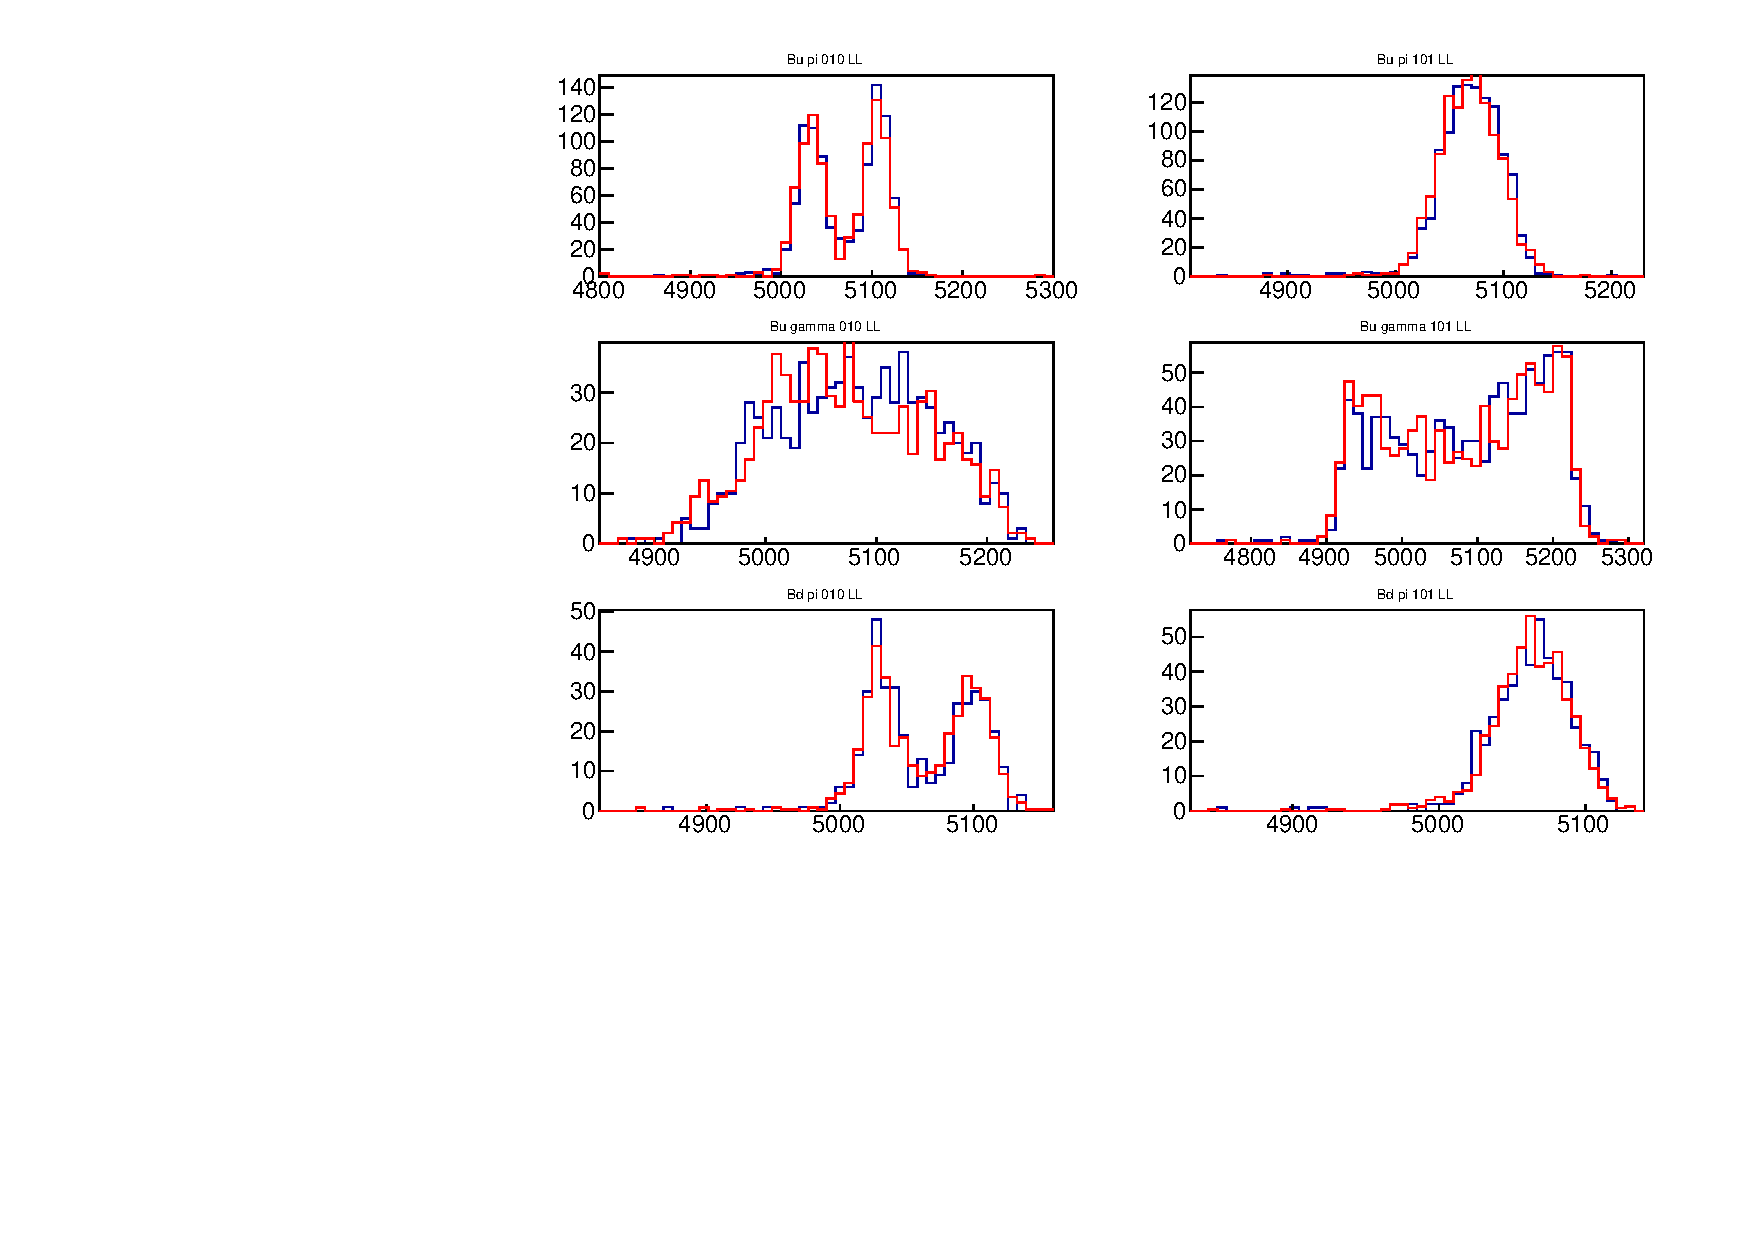
\includegraphics[width=\linewidth]{figures/compareMC/run1vsrun2MC_partreco_LL.pdf}
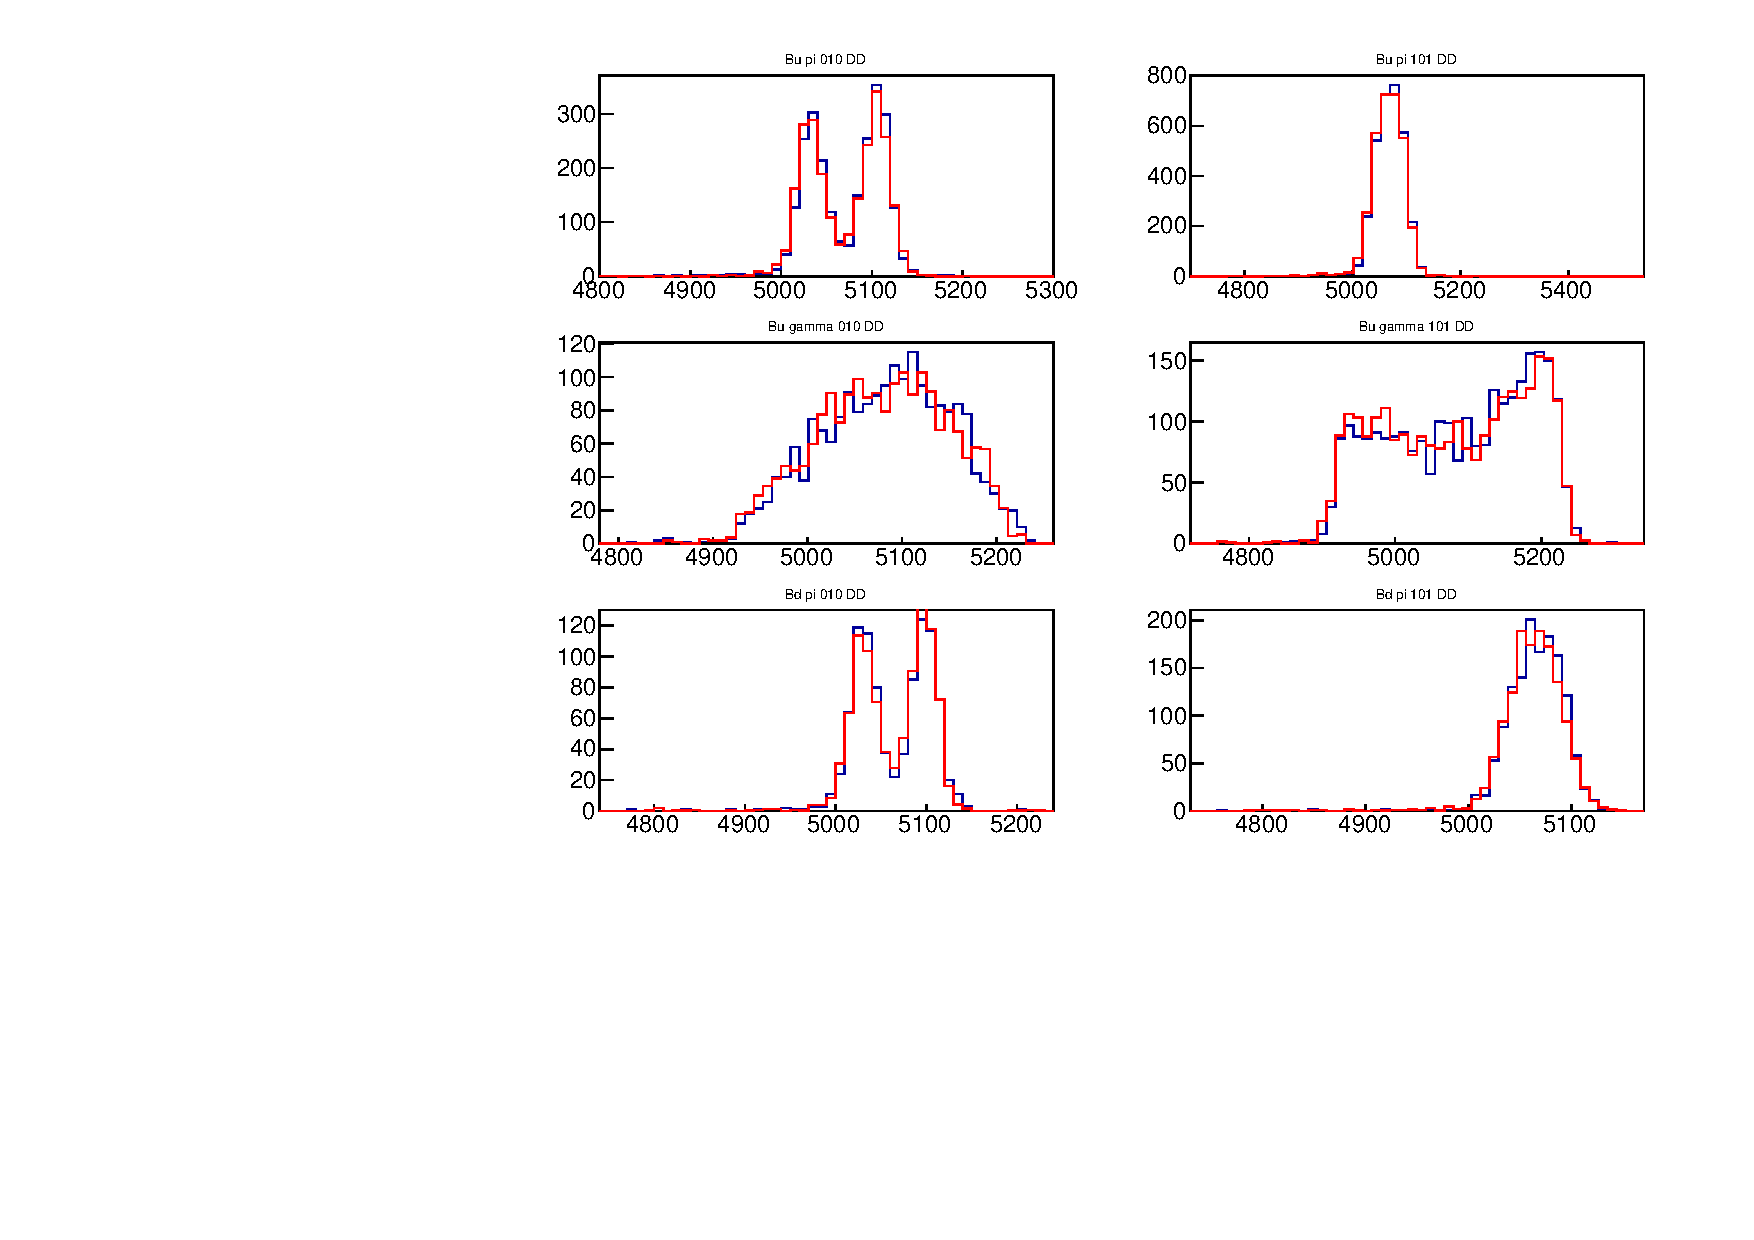
\includegraphics[width=\linewidth]{figures/compareMC/run1vsrun2MC_partreco_DD.pdf}
\caption{Comparison of partially reconstructed MC between Run 1 (blue) and 2015 (red). The different shapes correspond to different \Dstar\Kstar modes, descibed in Section \ref{sec:massfit:partreco}}
\label{parterecofits}
\end{figure}

The shapes are taken from simulation are fitted separately using the functions given by equations \ref{eqn:horns}, \ref{eqn:hill} and \ref{eqn:littlehorns}, the fits are shown in Figures \ref{partrecofitsLL} and \ref{partrecofitsDD}. All the parameters for these shapes are fixed in the mass fit from fits to simultated events. The values of these fixed parameters are given in Tables ?

\begin{table}[h]
\centering
\begin{tabular}{cccc}
Helicity of \Dstar & Missing particle & $\theta$ dependence & Function \\
\hline
0 & $\pi$ & $\left(x - \frac{a+b}{2}\right)^2$ & Horns, from Eq.~\ref{eqn:horns} \\
0 & \Pgamma & $-(x - a)(x - b)$ & Hill, from Eq.~\ref{eqn:hill} \\
$\pm$1 & $\pi$ & $-(x - a)(x - b)$ & Hill, from Eq.~\ref{eqn:hill} \\
$\pm$1 & \Pgamma & $\left(x - \frac{a+b}{2}\right)^2 + \left(\frac{a-b}{2}\right)^2$ & Little Horns, from Eq.~\ref{eqn:littlehorns} \\
\end{tabular}
\caption{Possible combinations of \Dstar helicity angle and missing particle and how this relates to the dependence on the helicity angle and the \B mass parameterisation}
\label{helicityamplitudes}
\end{table}

\begin{figure}[h]
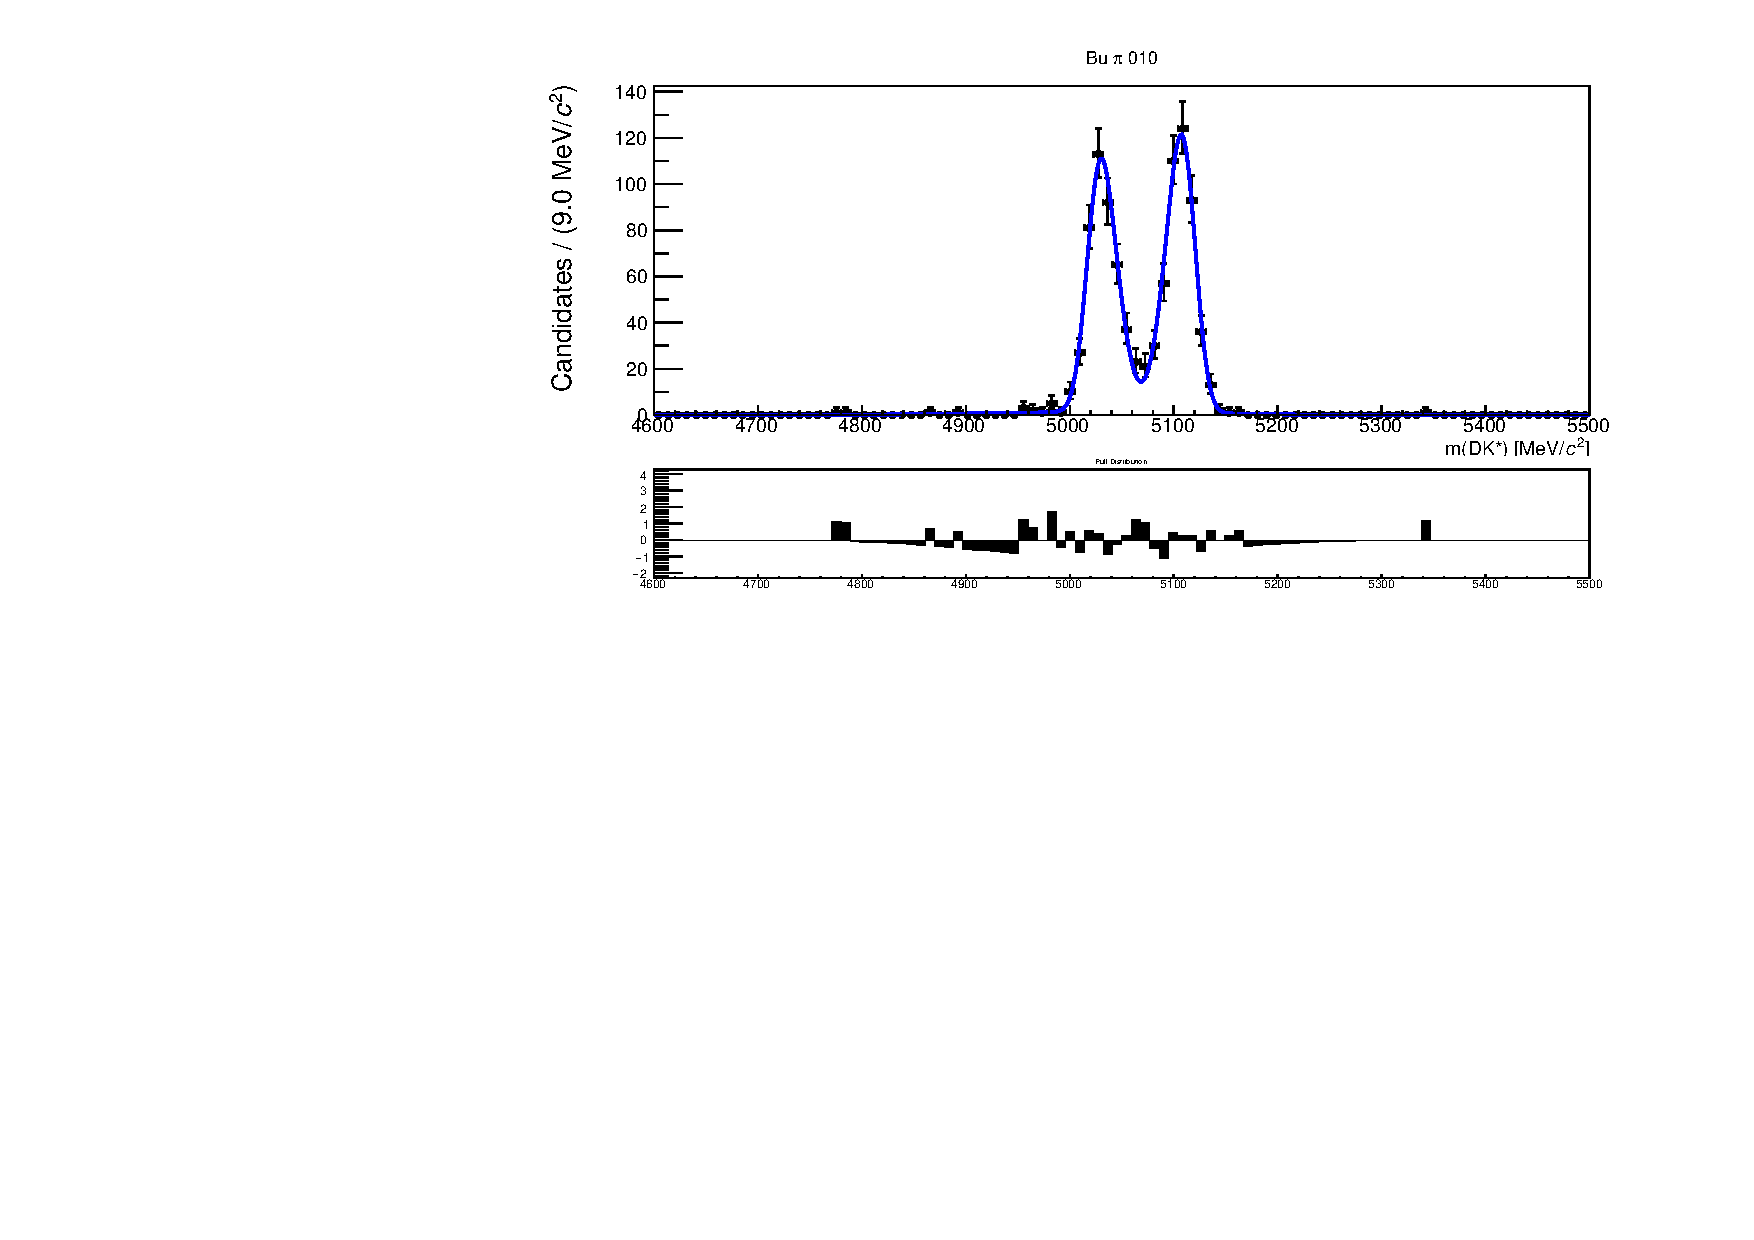
\includegraphics[width=0.5\linewidth]{figures/fitComponents/Bupi010_LL.pdf}
\put(-180,80) {(a)}
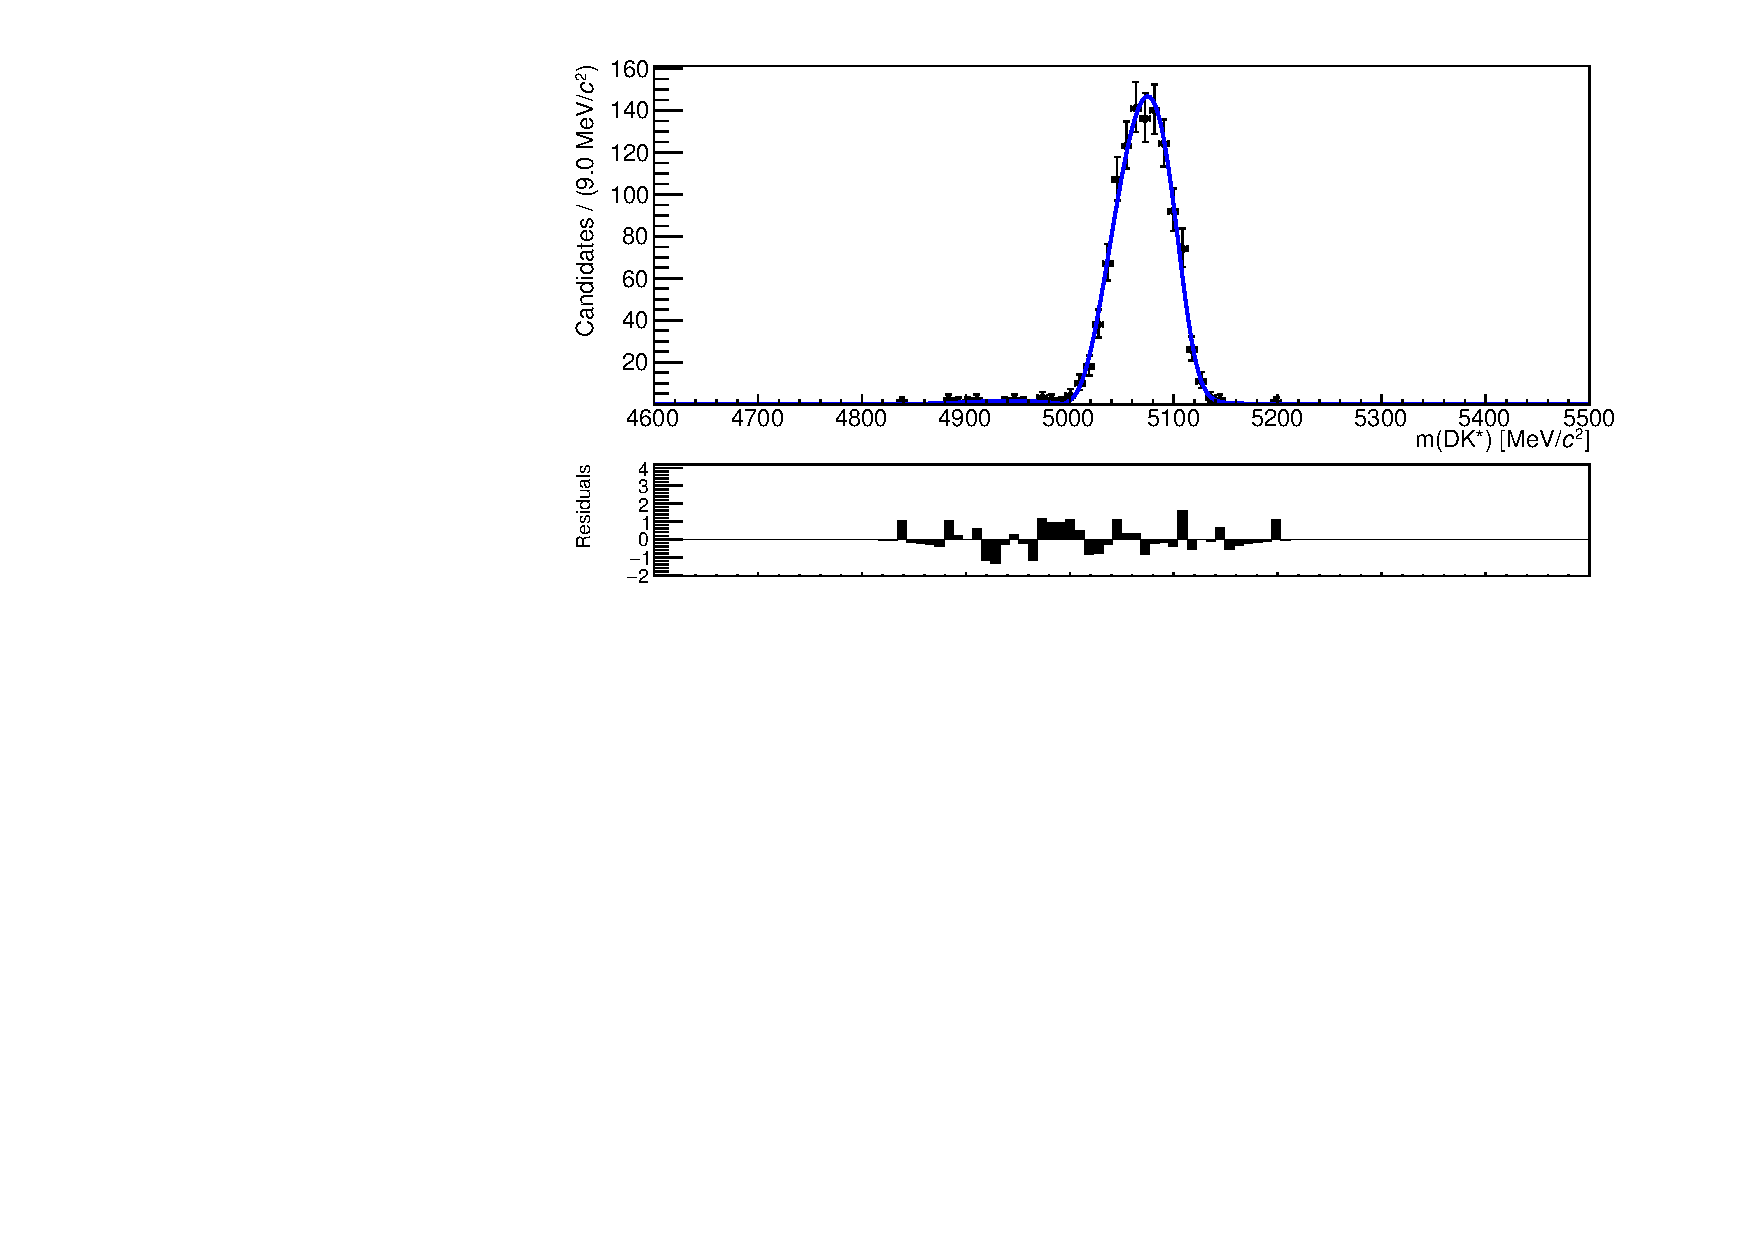
\includegraphics[width=0.5\linewidth]{figures/fitComponents/Bupi101_LL.pdf}
\put(-180,80) {(b)}
\hfill
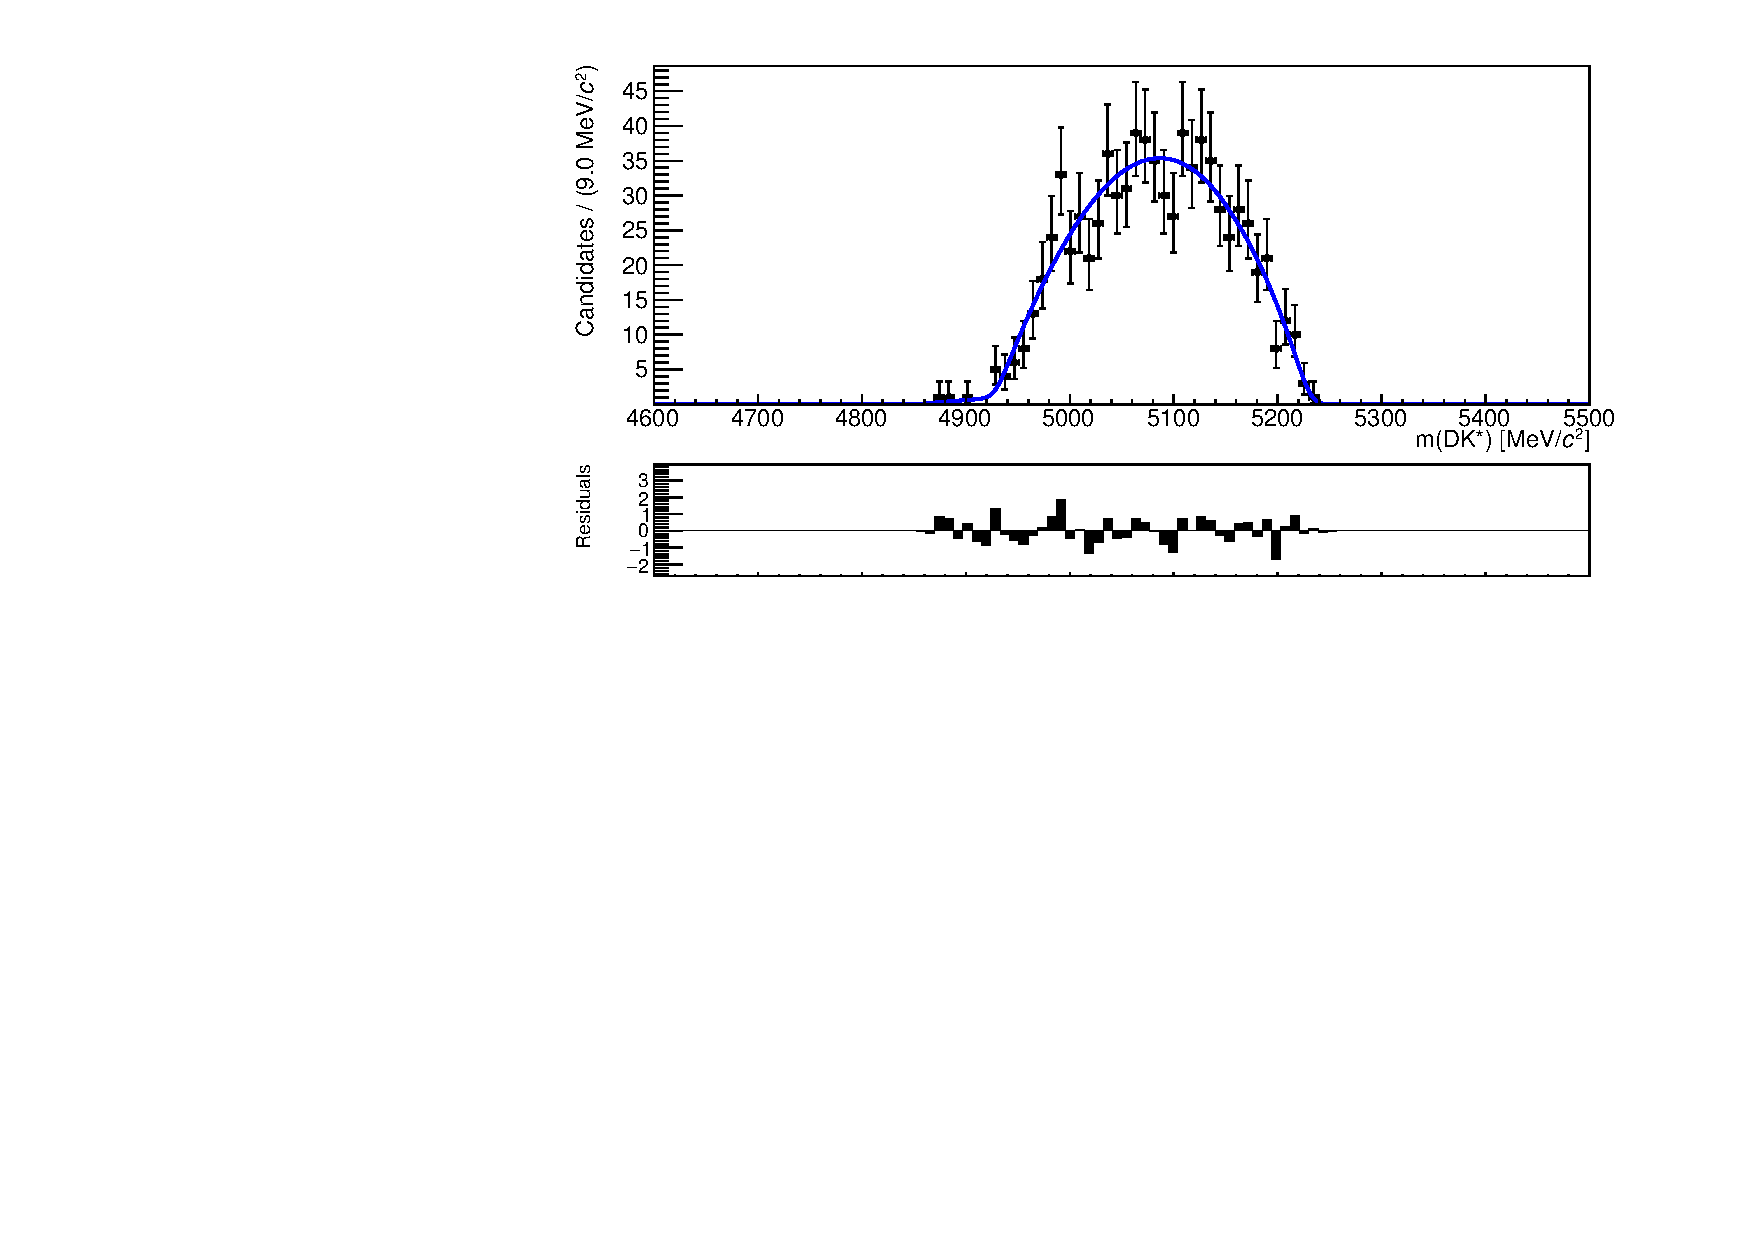
\includegraphics[width=0.5\linewidth]{figures/fitComponents/Bugamma010_LL.pdf}
\put(-180,80) {(c)}
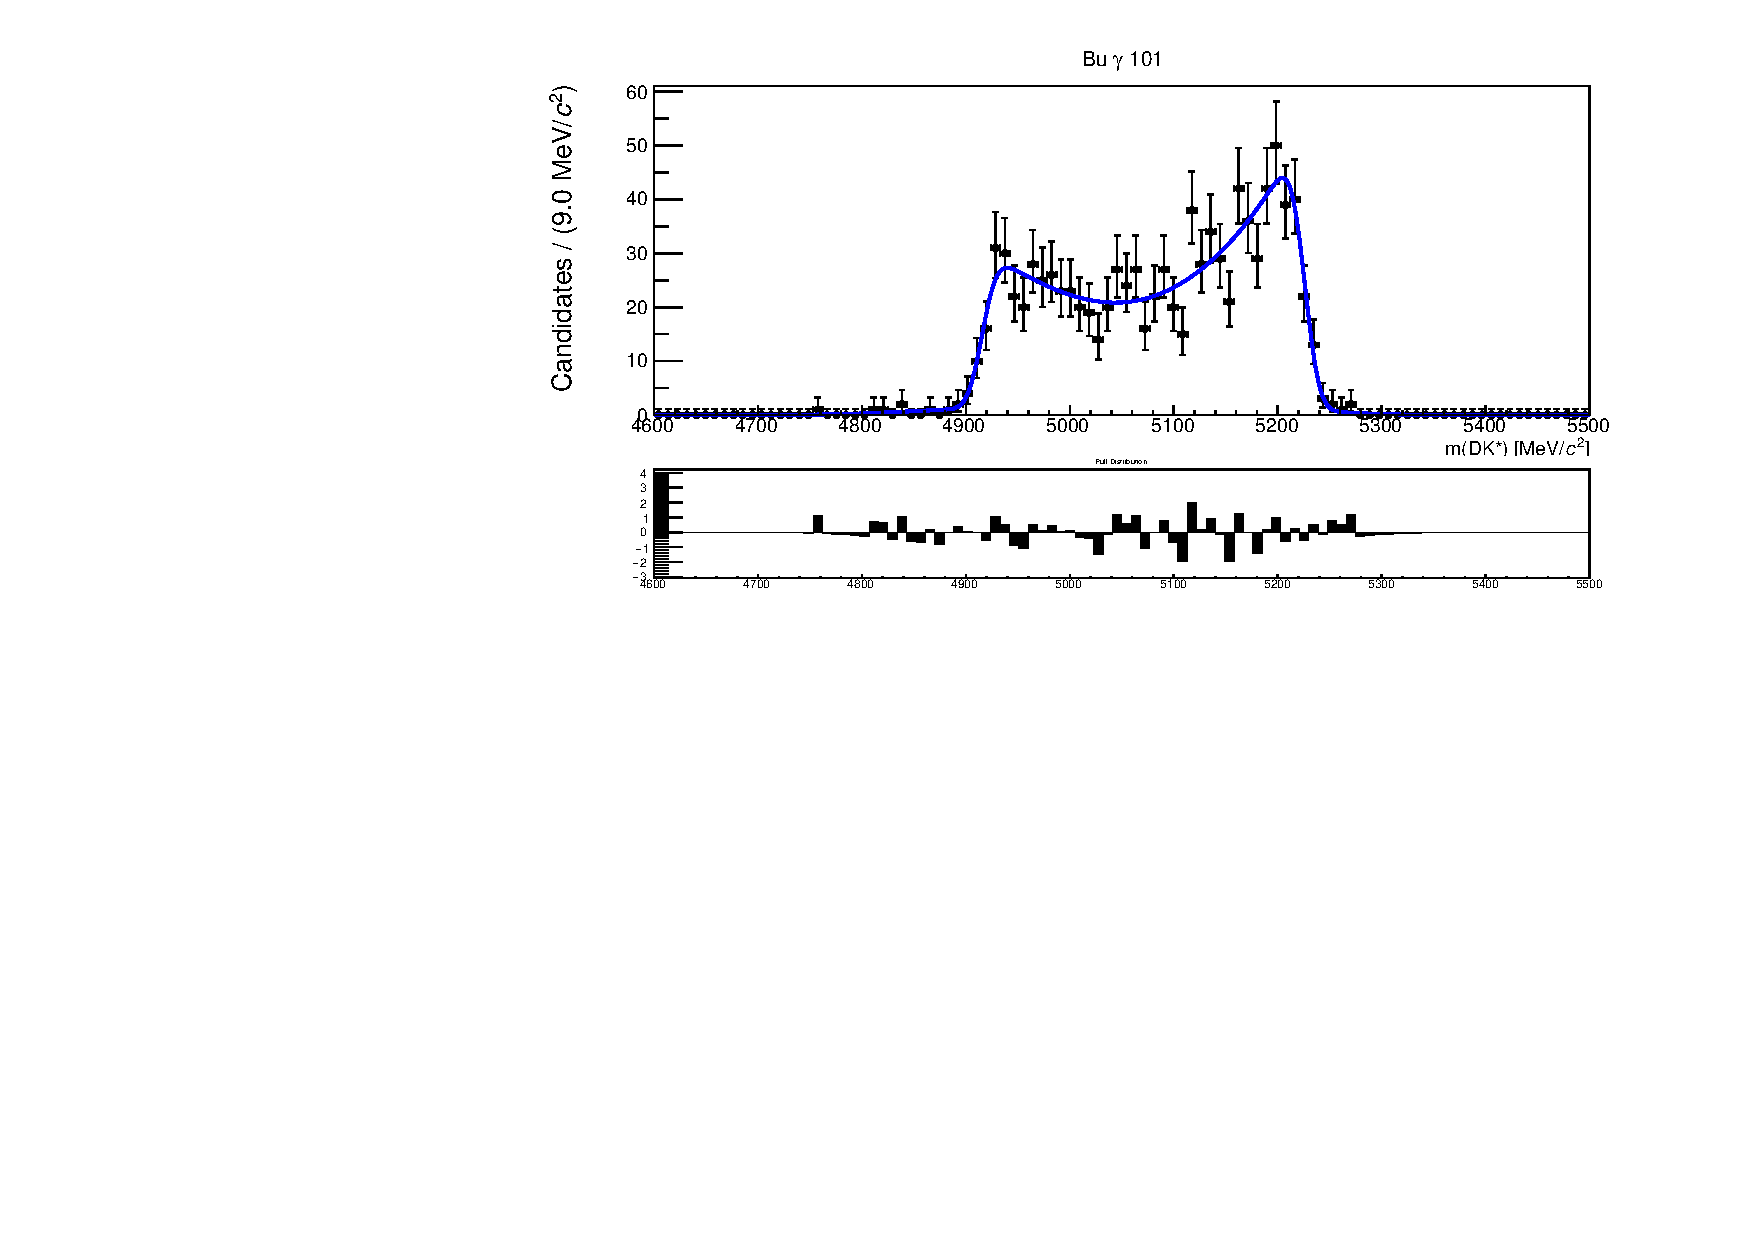
\includegraphics[width=0.5\linewidth]{figures/fitComponents/Bugamma101_LL.pdf}
\put(-180,80) {(d)}
\hfill
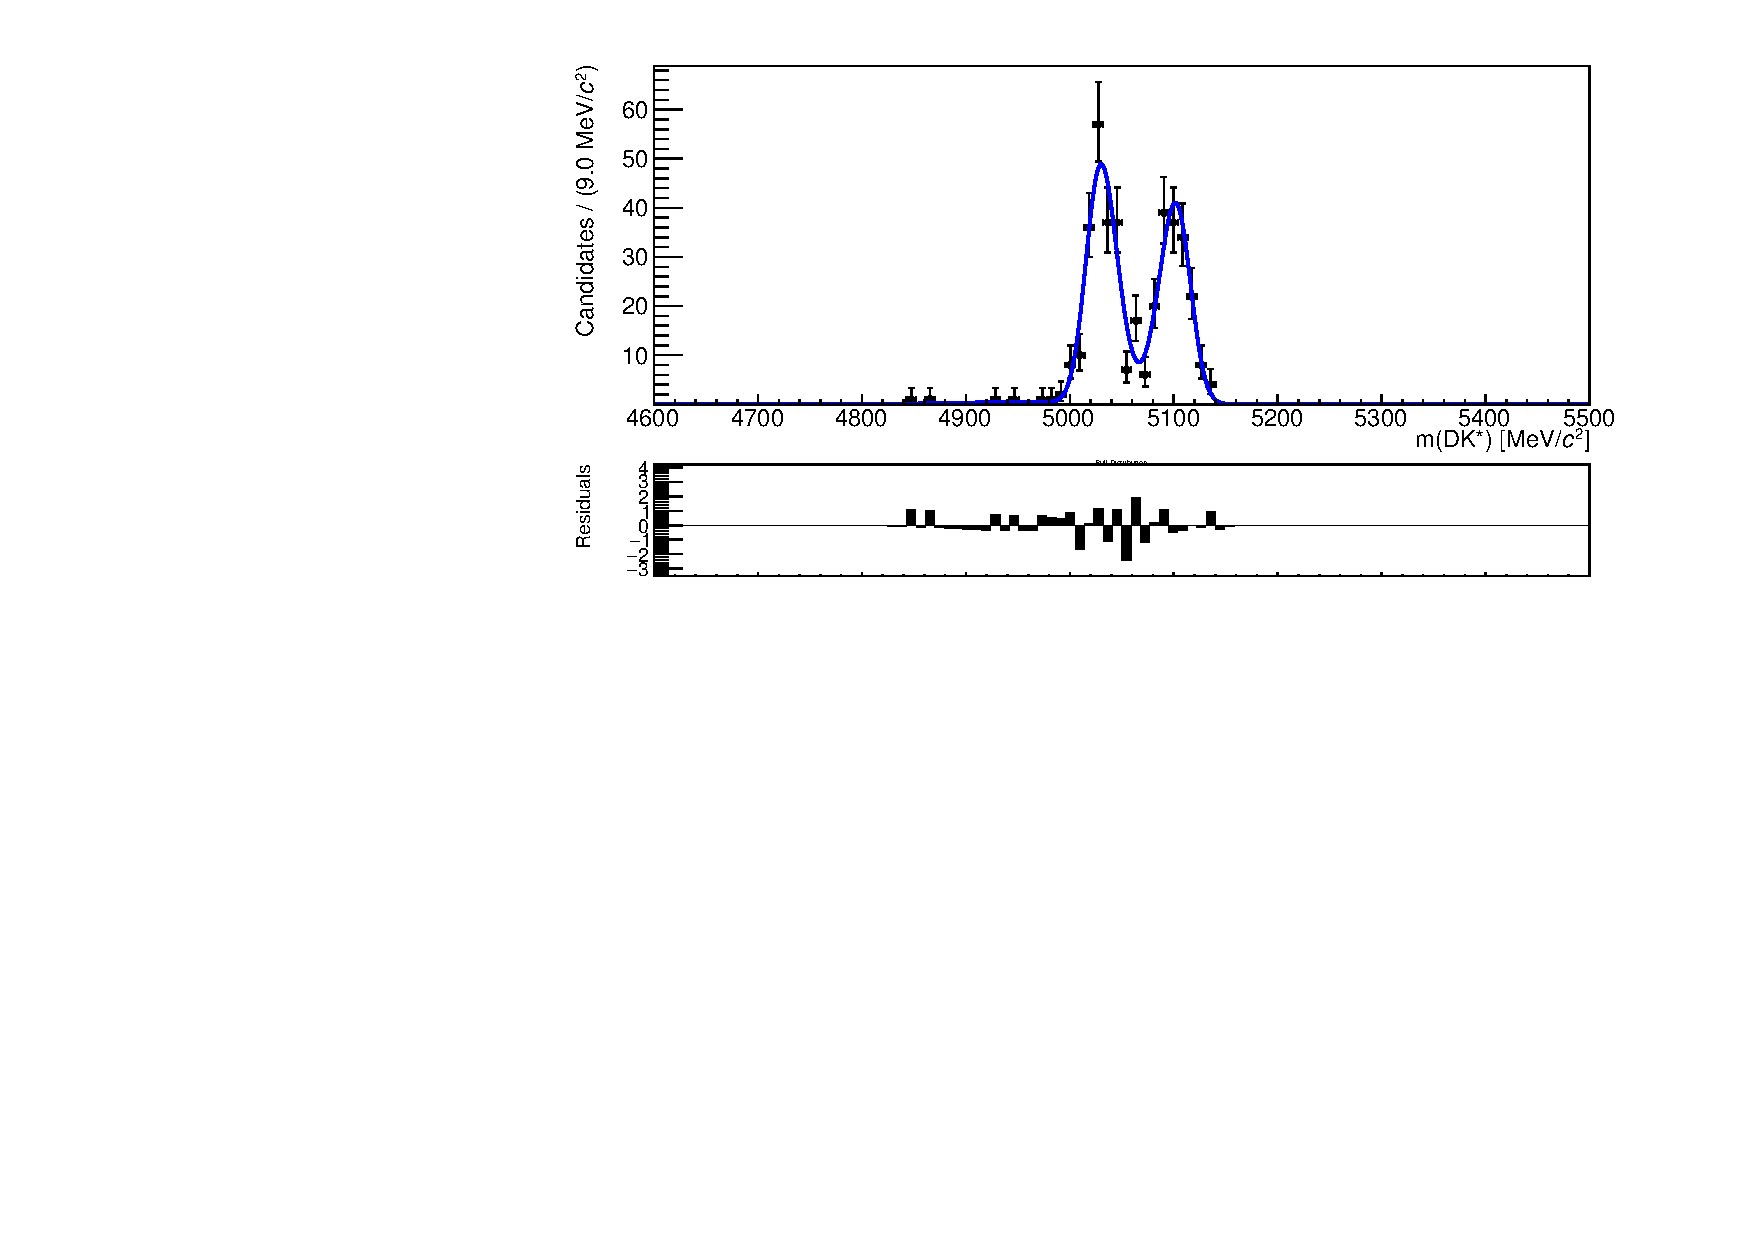
\includegraphics[width=0.5\linewidth]{figures/fitComponents/Bdpi010_LL.pdf}
\put(-180,80) {(e)}
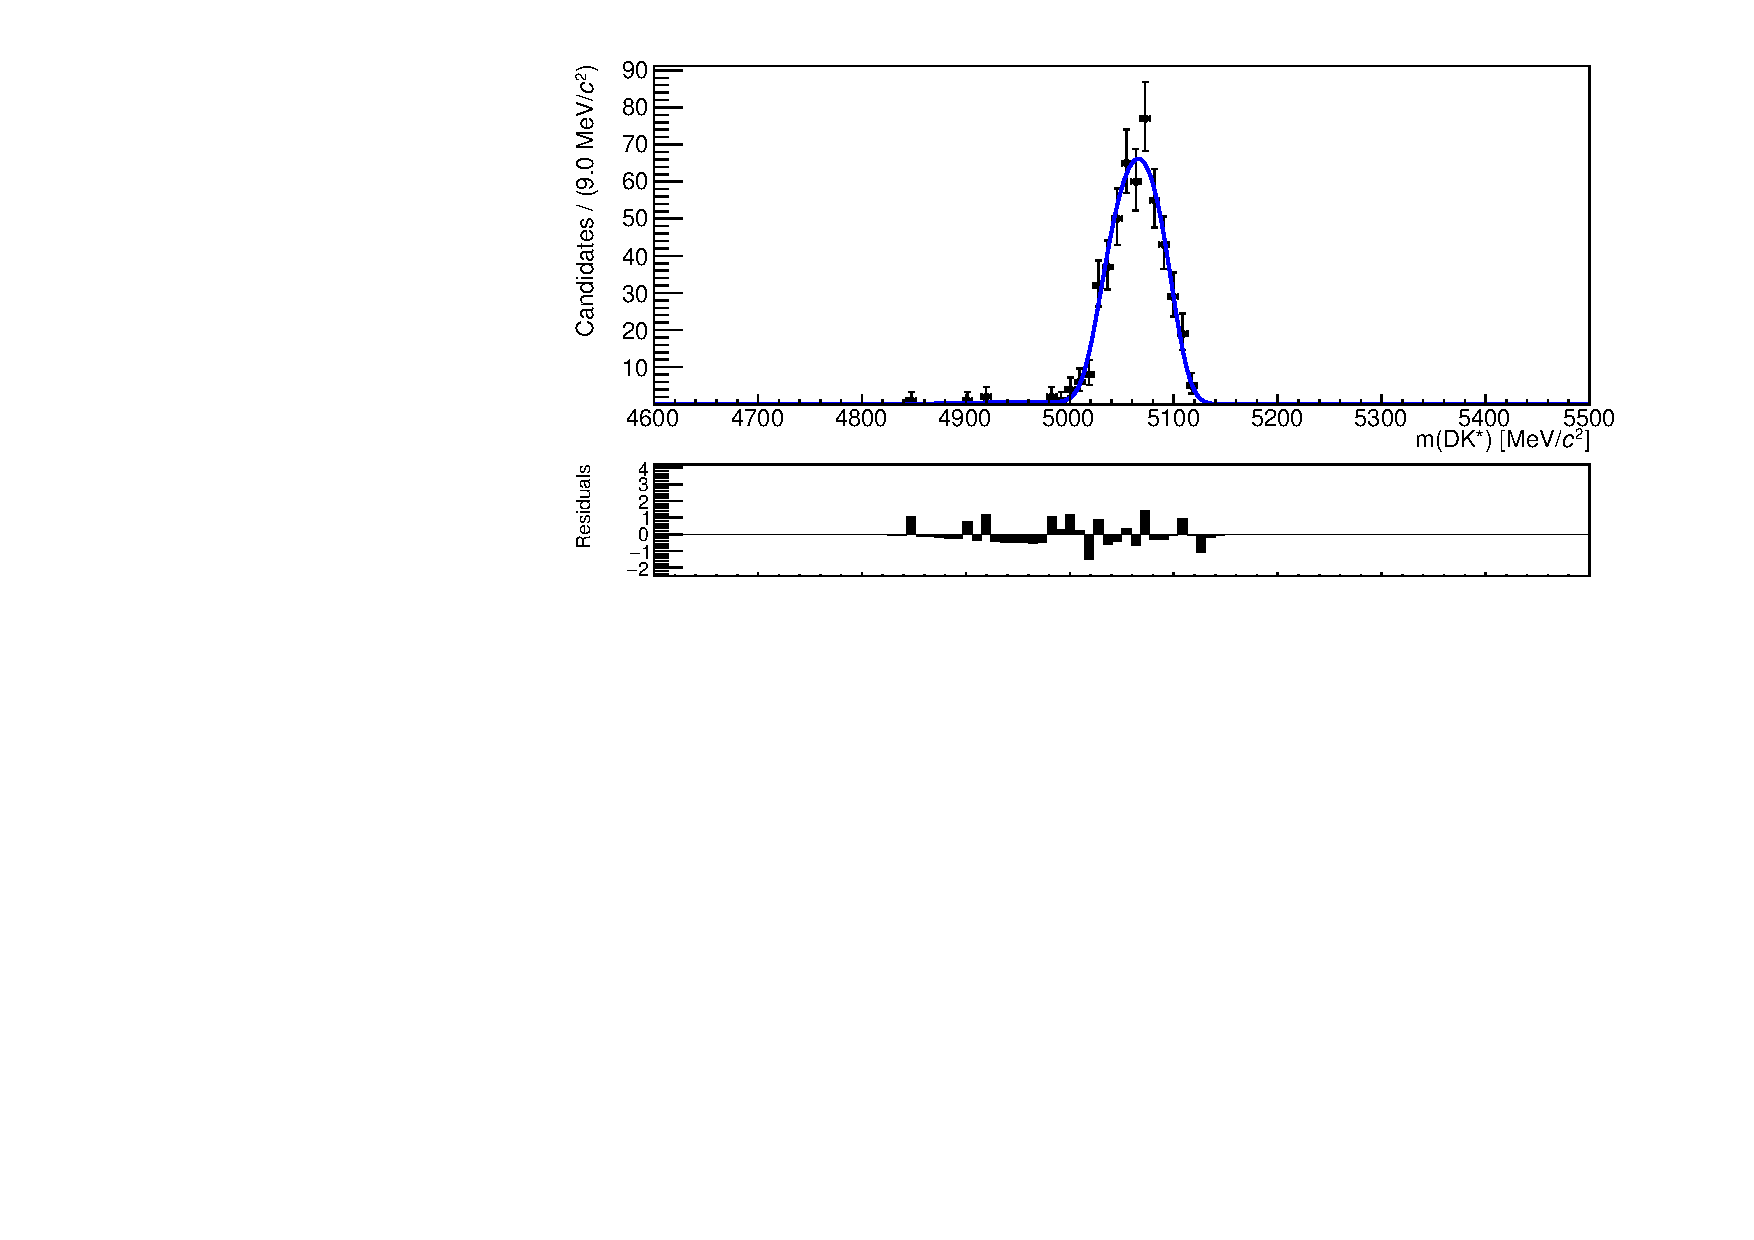
\includegraphics[width=0.5\linewidth]{figures/fitComponents/Bdpi101_LL.pdf}
\put(-180,80) {(f)}
\caption{Fit to $B \to D^*K^*$ \runone simulated samples in all the different modes for LL candidates (a) \decay{\Bm}{(\decay{\Dstarz}{\Dz[\piz]})\Kstarm} 0, (b) \decay{\Bm}{(\decay{\Dstarz}{\Dz[\piz]})\Kstarm} $\pm$1, (c) \decay{\Bm}{(\decay{\Dstarz}{\Dz[\gamma]})\Kstarm} 0, (d) \decay{\Bm}{(\decay{\Dstarz}{\Dz[\gamma]})\Kstarm} $\pm$1, (e) \decay{\Bd}{(\decay{\Dstarp}{\Dz[\pip]})\Kstarm} 0, and (f) \decay{\Bd}{(\decay{\Dstarp}{\Dz[\pip]})\Kstarm} $\pm$1}
\label{partrecofitsLL}
\end{figure}

\begin{figure}[h]
\includegraphics[width=0.5\linewidth]{figures/fitComponents/Bupi010_DD.pdf}
\put(-180,80) {(a)}
\includegraphics[width=0.5\linewidth]{figures/fitComponents/Bupi101_DD.pdf}
\put(-180,80) {(b)}
\hfill
\includegraphics[width=0.5\linewidth]{figures/fitComponents/Bugamma010_DD.pdf}
\put(-180,80) {(c)}
\includegraphics[width=0.5\linewidth]{figures/fitComponents/Bugamma101_DD.pdf}
\put(-180,80) {(d)}
\hfill
\includegraphics[width=0.5\linewidth]{figures/fitComponents/Bdpi010_DD.pdf}
\put(-180,80) {(e)}
\includegraphics[width=0.5\linewidth]{figures/fitComponents/Bdpi101_DD.pdf}
\put(-180,80) {(f)}
\caption{Fit to $B \to D^*K^*$ \runone simulated samples in all the different modes for DD candidates (a) \decay{\Bm}{(\decay{\Dstarz}{\Dz[\piz]})\Kstarm} 0, (b) \decay{\Bm}{(\decay{\Dstarz}{\Dz[\piz]})\Kstarm} $\pm$1, (c) \decay{\Bm}{(\decay{\Dstarz}{\Dz[\gamma]})\Kstarm} 0, (d) \decay{\Bm}{(\decay{\Dstarz}{\Dz[\gamma]})\Kstarm} $\pm$1, (e) \decay{\Bd}{(\decay{\Dstarp}{\Dz[\pip]})\Kstarm} 0, and (f) \decay{\Bd}{(\decay{\Dstarp}{\Dz[\pip]})\Kstarm} $\pm$1}
\label{partrecofitsDD}
\end{figure}

As there are six shapes in this low mass region of the mass fit, from 4900-5230 MeV, it is necessary to fix some yields in order to have a stable fit. The total partially reconstructed PDF is given in Equation \ref{partrecofunction}.
\begin{equation}
P_{partreco} = f_0P_0 + (1 - f_0)P_{\pm 1}
\label{partrecofunction}
\end{equation}
where $P_0$ and $P_{\pm 1}$, which represent the total PDF for the \Dstar helicity states 0 and $\pm$1 respectively, are given by
\begin{align*}
P_0 &= P^{Bu,\pi}_0 + c^{Bu,\gamma}_0P^{Bu,\gamma}_0 + c^{Bd,\pi}_0P^{Bd,\pi}_0 \\
P_{\pm 1} &= P^{Bu,\pi}_{\pm 1} + c^{Bu,\gamma}_{\pm 1}P^{Bu,\gamma}_{\pm 1} + c^{Bd,\pi}_{\pm 1}P^{Bd,\pi}_{\pm 1} \text{ .}
\end{align*}
The yield ratios between \decay{\Bm}{(\decay{\Dstarz}{\Dz[\piz]})\Kstarm}, \decay{\Bm}{(\decay{\Dstarz}{\Dz[\gamma]})\Kstarm} and \decay{\Bd}{(\decay{\Dstarp}{\Dz[\pip]})\Kstarm} are fixed separately for the 0 and $\pm$1 helicity states of the \Dstar. These yield ratios, $c^{Bu,\gamma}_0$, $c^{Bd,\pi}_0$, $c^{Bu,\gamma}_{\pm 1}$ and $c^{Bd,\pi}_{\pm 1}$, that are fixed in the fit to the values given in Table \ref{fixedyieldratios}, are obtained from a ratio of braching fractions and selection efficiencies, an example calculation is given in Equation \ref{partrecoexample}. This calculation is performed for each of the ratios listed in Table \ref{fixedyieldratios}. Branching fractions for the partially reconstructed decays are given in Table \ref{partrecoBRs}. Simulated events are generated for each of the modes and the values of $\epsilon_{sel}$, used in Equation \ref{partrecoexample}, are given by the fraction of simulated events passing the selection.

\begin{multline}
\frac{N(\decay{\B}{(\decay{\Dstar}{\Dz\piz})\Kstar}\ 0)}{N(\decay{\B}{(\decay{\Dstar}{\Dz\gamma})\Kstar}\ 0)} = \frac{\mathcal{B}(\decay{\B}{(\decay{\Dstar}{\Dz\piz})\Kstar})}{\mathcal{B}(\decay{\B}{(\decay{\Dstar}{\Dz\gamma})\Kstar})} \\
\times \frac{\epsilon_{sel}(\decay{\B}{(\decay{\Dstar}{\Dz\piz})\Kstar}\ 0)}{\epsilon_{sel}(\decay{\B}{(\decay{\Dstar}{\Dz\gamma})\Kstar}\ 0)}
\label{partrecoexample}
\end{multline}

\begin{table}[h]
\centering
\begin{tabular}{c|c}
Mode & Branching ratio \\
\hline
\decay{\Bm}{(\decay{\Dstarz}{\Dz[\piz]})\Kstarm} & $(5.0 \pm 0.9) \times 10^{-4}$ \\
\decay{\Bm}{(\decay{\Dstarz}{\Dz[\gamma]})\Kstarm} & $(3.1 \pm 0.6) \times 10^{-4}$ \\
\decay{\Bd}{(\decay{\Dstarp}{\Dz[\pip]})\Kstarm} & $(2.2 \pm 0.4) \times 10^{-4}$ \\
\end{tabular}
\caption{Branching ratios for the different partially reconstructed decay modes~\cite{PDG2014}}
\label{partrecoBRs}
\end{table}

\begin{table}[h]
\centering
\begin{tabular}{ccc}
\hline
& LL & DD \\
\hline
$c^{Bu,\gamma}_0$ & $0.53 \pm 0.14$ & $0.51 \pm 0.14$ \\[3mm]
$c^{Bd,\pi}_0$ & $0.38 \pm 0.14$ & $0.37 \pm 0.14$ \\[3mm]
$c^{Bu,\gamma}_{\pm 1}$ & $0.53 \pm 0.14$ & $0.51 \pm 0.14$ \\[3mm]
$c^{Bd,\pi}_{\pm 1}$ & $0.38 \pm 0.14$ & $0.38 \pm 0.14$ \\[3mm]
\hline
\end{tabular}
\caption{Yield ratios fixed in the mass fit for the partically reconstructed backgrounds}
\label{fixedyieldratios}
\end{table}

Other backgrounds investigated in this analysis, but not included in the mass fit are discussed in Section \ref{sec:backgrounds}.


\subsection{Mass fit to the data in the favoured modes}
\label{sec:massfit:fit}

A fit to the invariant B mass in the \kpi and \kpipipi favoured mode is performed using the shapes discussed in Sections \ref{sec:massfit:signal}, \ref{sec:massfit:combinatorial} and \ref{sec:massfit:partreco}. The total PDF is given by
\begin{equation}
P_{tot} = N_{sig}P_{sig} + N_{comb}P_{comb} + N_{dstkst}P_{dstkst} \text{ ,}
\end{equation}
where $N_{sig}$, $N_{comb}$ and $N_{dstkst}$ are the yields of the signal, combinatoric and partially reconstructed yields restpectively. The signal PDF, $P_{sig}$, is given by Equation~\ref{DCBshape}, the partially reconstructed PDF, $P_{dstkst}$, is given by Equation~\ref{partrecofunction} and the combintorial PDF is an exponential, $P_{comb} = e^{\beta m}$, where the slope parameter $\beta$ is able to vary in the fit. The yield of the signal and combinatoric shape, $N_{sig}$ and $N_{comb}$, are left to vary without constraint. Other parameters allowed to vary are the peak position, $\mu$, and width, $\sigma$, of the signal PDF. The only parameters able to vary in the partially reconstructed background are the yield ratio between the 0 and $\pm$1 amplitudes, $f_0$, and the overall yield, $N_{dstkst}$.

Figures \ref{massfitskpi} and \ref{massfitsk3pi} show the fits to the invariant B mass distribution in the \kpi and \kpipipi favoured mode respectively for LL and DD candidates in both Run 1 and Run 2. The estimated \kpi signal yield extracted from these fits for Run 1 is $220 \pm 16$ for LL and $505 \pm 24$ for DD, and for Run 2 is $388 \pm 21$ for LL and $901 \pm 33$ for DD. The full fit results for the two-body \kpi fits are shown in Table \ref{fitresultskpi}. For the \kpipipi mode, the estimated signal yield extracted from these fits for Run 1 is $87 \pm 10$ for LL and $205 \pm 16$ for DD, and for Run 2 is $215 \pm 15$ for LL and $516 \pm 25$ for DD. The full fit results for the four-body \kpipipi fits are shown in Table \ref{fitresultsk3pi}.

\begin{figure}
\centering
\subfloat[Run 1 LL]{\includegraphics[width=0.7\linewidth]{figures/fitComponents/massFit_LL_KPi_run1.pdf}}
\vspace{-12pt}
\hfill
\subfloat[Run 1 DD]{\includegraphics[width=0.7\linewidth]{figures/fitComponents/massFit_DD_KPi_run1.pdf}}
\vspace{-12pt}
\hfill
\subfloat[Run 2 LL]{\includegraphics[width=0.7\linewidth]{figures/fitComponents/massFit_LL_KPi_run2.pdf}}
\vspace{-12pt}
\hfill
\subfloat[Run 2 DD]{\includegraphics[width=0.7\linewidth]{figures/fitComponents/massFit_DD_KPi_run2.pdf}}
\caption{Fits to the invariant B mass distribution in the \kpi favoured mode}
\label{massfitskpi}
\end{figure}

\begin{figure}
\centering
\subfloat[Run 1 LL]{\includegraphics[width=0.7\linewidth]{figures/fitComponents/massFit_LL_KPiPiPi_run1.pdf}}
\vspace{-12pt}
\hfill
\subfloat[Run 1 DD]{\includegraphics[width=0.7\linewidth]{figures/fitComponents/massFit_DD_KPiPiPi_run1.pdf}}
\vspace{-12pt}
\hfill
\subfloat[Run 2 LL]{\includegraphics[width=0.7\linewidth]{figures/fitComponents/massFit_LL_KPiPiPi_run2.pdf}}
\vspace{-12pt}
\hfill
\subfloat[Run 2 DD]{\includegraphics[width=0.7\linewidth]{figures/fitComponents/massFit_DD_KPiPiPi_run2.pdf}}
\caption{Fits to the invariant B mass distribution in the \kpipipi favoured mode}
\label{massfitsk3pi}
\end{figure}

\begin{table}[h]
\centering
\resizebox{\textwidth}{!}{
\begin{tabular}{l|cc|cc}
\hline
& \multicolumn{2}{c}{Run 1} & \multicolumn{2}{c}{Run 2} \\
& LL & DD & LL & DD \\
\hline
$\beta$ & $(-4.8 \pm 0.5) \times 10^{-3}$ & $(-2.8 \pm 0.3) \times 10^{-3}$ & $(-4.4 \pm 0.5) \times 10^{-3}$ & $(-2.5 \pm 0.2) \times 10^{-3}$ \\
$f_0$ & $0.15 \pm 0.08$ & $0.12 \pm 0.05$ & $0.18 \pm 0.05$ & $0.06 \pm 0.04$ \\
$\mu$ & $5280.7 \pm 0.8$ & $5280.7 \pm 0.6$ & $5278.5 \pm 0.8$ & $5278.6 \pm 0.5$ \\
$N_{comb}$ & $167 \pm 20$ & $472 \pm 34$ & $223 \pm 24$ & $1100 \pm 50$ \\
$N_{dstkst}$ & $338 \pm 23$ & $810 \pm 36$ & $654 \pm 31$ & $1397 \pm 49$ \\
$N_{sig}$ & $220 \pm 16$ & $505 \pm 24$ & $388 \pm 21$ & $901 \pm 33$ \\
$\sigma$ & $10.2 \pm 0.7$ & $11.5 \pm 0.5$ & $12.2 \pm 0.6$ & $11.5 \pm 0.4$ \\
\hline
\end{tabular}}
\caption{Fit results from the \kpi favoured mode for LL and DD candidates, corresponding to the fits in Figure \ref{massfitskpi}. The parameter $\beta$ is the combinatoric background slope, $f_0$ is the yield ratio between 010 and 101 helicity amplitudes, $\sigma$ is the floating width of the signal shape, and $N_{sig}$, $N_{comb}$ and $N_{dstkst}$ are the yields of signal, combinatoric background and partially reconstructed decays respectively}
\label{fitresultskpi}
\end{table}

\begin{table}[h]
\centering
\resizebox{\textwidth}{!}{
\begin{tabular}{l|cc|cc}
\hline
& \multicolumn{2}{c}{Run 1} & \multicolumn{2}{c}{Run 2} \\
& LL & DD & LL & DD \\
\hline
$\beta$ & $(-5.2 \pm 1.1) \times 10^{-3}$ & $(-2.3 \pm 0.4) \times 10^{-3}$ & $(-4.4 \pm 0.5) \times 10^{-3}$ & $(-2.1 \pm 0.2) \times 10^{-3}$ \\
$f_0$ & $0.26 \pm 0.11$ & $0.20 \pm 0.08$ & $0.15 \pm 0.07$ & $0.16 \pm 0.05$ \\
$\mu$ & $5281.3 \pm 1.3$ & $5283.9 \pm 0.9$ & $5278.7 \pm 1.0$ & $5277.7 \pm 0.7$ \\
$N_{comb}$ & $50 \pm 12$ & $252 \pm 24$ & $168 \pm 20$ & $707 \pm 40$ \\
$N_{dstkst}$ & $154 \pm 15$ & $317 \pm 24$ & $342 \pm 23$ & $914 \pm 40$ \\
$N_{sig}$ & $102 \pm 10$ & $226 \pm 16$ & $244 \pm 16$ & $578 \pm 27$ \\
$\sigma$ & $11.4 \pm 1.0$ & $11.3 \pm 0.8$ & $12.9 \pm 0.8$ & $13.1 \pm 0.6$ \\
\hline
\end{tabular}}
\caption{Fit results from the \kpipipi favoured mode for LL and DD candidates, corresponding to the fits in Figure \ref{massfitsk3pi}. The parameter $\beta$ is the combinatoric background slope, $f_0$ is the yield ratio between 010 and 101 helicity amplitudes, $\sigma$ is the floating width of the signal shape, and $N_{sig}$, $N_{comb}$ and $N_{dstkst}$ are the yields of signal, combinatoric background and partially reconstructed decays respectively}
\label{fitresultsk3pi}
\end{table}

An additional source of background coming from the decay \decay{\Lb}{\Lc(pK\pip)\Kstarm} is included in the simultaneous fit for the \decay{\Bm}{\D(\Kp\Km)\Kstarm} mode, as discussed in detail in Section \ref{sec:backgrounds:Lb2LcKst}. The yield of \decay{\Lb}{\Lc(pK\pip)\Kstarm} compared to the signal yield in the \decay{\Bm}{\D(\Km\pip)\Kstarm} mode is allowed to vary.

%%%%%%%%%%%%%%%%%%%%%%%%
\subsection{Choice of fit range}
\label{sec:massfit:range}	

Fixing the relative yields for the partially reconstructed shapes, as in Table \ref{fixedyieldratios}, is possible only under the assumption that \CP violation is negligible. This is a reasonable assumption for the favoured \kpi decay where we do not expect \CP violation, however in the other \D final states, for example \pik, there is expected \CP violation in the partially reconstructed background for which the parameters are entirely unknown. Therefore, it is not possible make any constraints at all in these modes. The fit that would result from fitting six individual yields with an order of magnitude less data would be unstable and this lack of constraint in the low mass region would lead to a large amount of freedom in the combinatoric, significantly affecting the signal yield. 

The overlap of the partially reconstructed and signal peaks is very small. There are a number of advantages to raising the lower range of the mass parameterisation up to 5230 \mev, which only removes 0.4\% of signal. The advantages include avoiding the need to fit the various partially reconstructed yields in each of the other D decays modes. These cannot use the same assumptions and fractions as determined in the Cabibbo-favoured mode due to expected CP violation. Further benefits are that low level broad backgrounds that may be present in the range 4900 - 5200 \mev do not need to considered as sources of systematics uncertainty. The shape and yield of the small amount of partially reconstructed background present in all \D decay categories above 5230 \mev is determined and fixed from the fits to data of the \kpi and \kpipipi decays, taking into account the smaller branching fractions of the \D decays. It is less than an event for all the CP violating modes. Due to the assumptions present in the initial fit, uncertainties in the yield and shape and possible asymmetries in distribution between \Bp and \Bm are evaluated as systematic uncertainties. This systematic uncertainty is dealt with in Section \ref{sec:systematics:partreco}.


\clearpage
